%============================================================================
% LaTeX File
% Daniel J. Greenhoe
%============================================================================
%--------------------------------------
% Compile control
%--------------------------------------




%\includeonly{../common/preface,../common/intro}
%\includeonly{../common/netdet}

\documentclass [12pt,twoside,titlepage,final,openbib]{book}
%\documentclass [12pt,twoside,titlepage,draft,openbib]{book}

%--------------------------------------
% Style Packages
%--------------------------------------
\usepackage{../common/sty/packages}  % common packages
\usepackage{../common/sty/dan}       % common definitions
\usepackage{../common/sty/math}      % common mathematics definitions
\usepackage{../dcsd/dcsd}                    % digital communications
\usepackage{../common/sty/language}  % Chinese language support

%--------------------------------------
% environment setup
%--------------------------------------
\renewcommand{\bullet}{\ensuretext{\scriptsize\mancube}}

%--------------------------------------
% Headers and Footers
%--------------------------------------
 \pagestyle{fancy}           % fancy headers from package <fancyhdr>
 \dateShort

 \fancyhf[HEL]    {\footnotesize \leftmark}
 \fancyhf[HOL,HER]{\scriptsize\personal\textcolor{clr:signature}{Daniel J. Greenhoe} \footnotesize\zhthw{\textcolor{clr:signature}{(柯晨光)}}}
 \fancyhf[HOC,HEC]{}
 \fancyhf[HOR]    {\footnotesize \rightmark}
 \fancyhf[FOL,FER]{\scriptsize \today}
 \fancyhf[FOC,FEC]{page \thepage\hspace{1ex}{\scriptsize(of \pageref{doc:end} pages)}}
 \fancyhf[FOR,FEL]{\color[rgb]{0,0,1}\scriptsize Statistical Signal Processing\\\url{http://banyan.cm.nctu.edu.tw/~dgreenhoe/ssp/index.html}}
 %        |||
 %        |||______ L=left       C=center     R=right
 %        ||_______ E=even page  O=odd page
 %        |________ H=header     F=footer

 \renewcommand{\headrulewidth}{0.4pt}
 \renewcommand{\footrulewidth}{0pt}
 \renewcommand{\headrule}{\color[cmyk]{0,0,1,0}\rule[0pt]{\textwidth}{2pt}}

\makeindex        % make the index
%----------------------------------------------------------------------------
% Body
%----------------------------------------------------------------------------
\begin{document}
%\frontmatter
\VerbatimFootnotes   % macro to allow verbatim in footnotes (used with fancyvrb package)

%\multfootsep{;}                      % multiple footnote separator -- does not seem to work
%--------------------------------------
\begin {titlepage}
%--------------------------------------
\begin{center}
%\vfill

\begin{center}
  {\Huge Statistical Signal Processing}
\end{center}

\vfill
  by Daniel J. Greenhoe \zht{(柯晨光)}
\vfill

\begin{center}%
\begin{fsL}%
\setlength{\unitlength}{\textwidth/1600}%
\begin{picture}(1600,800)(0,0)%
  %\color[gray]{0.5}\graphpaper[100](0,0)(1600,800)%
  \thicklines%
  \color{blue}%
  \put(300,0){\includegraphics*[height=8\tw/16, width=8\tw/16, clip=true]{../common/mandel.eps}}%
  \put(100,400){\includegraphics*[height=3\tw/16, clip=true]{diver.eps}}%
  \put(1000,400){\includegraphics*[width=7\tw/16, clip=true]{../common/whale.eps}}%
  %\qbezier(0,10)(1,6.95)(2,3.9)%
  %\qbezier(8,10)(7,7.2)(6,4.4)%
  %\qbezier(4.5,3.2)(4.25,6.6)(4,10)%
  %\qbezier(3.5,5)(3.5,5.55)(3.5,6.1)%
\end{picture}%
\end{fsL}%
\end{center}%
\vfill
\cleartooddpage
\hspace{1pt}
\vfill
   \begin{tabular}{lll}
      title:        & Statistical Signal Processing Structure and Design\\
      author:       & \href{http://www.geocities.com/dgreenhoe/index.html}{Daniel J. Greenhoe  \zht{(柯晨光)}},\footnotemark student\\
      series:       & Mathematical Structure and Design \\
      number:       & 2 \\
      institution:  & \href{http://www.nctu.edu.tw/}{National Chiao-Tung University   (\zht{國立交通大學})}\footnotemark \\
      department:   & \href{http://www.cm.nctu.edu.tw}{Telecommunications Engineering   (\zht{電信工程學系})}\footnotemark \\
      email         & \href{mailto:dgreenhoe@yahoo.com}{dgreenhoe@yahoo.com} \\
%     email:        & \url{dgreenhoe@banyan.cm.nctu.edu.tw} \\
%     web:          & \url{http://www.geocities.com/dgreenhoe/}  \\
      web:          & \url{http://banyan.cm.nctu.edu.tw/~dgreenhoe/ssp/index.html}  \\
      time:         & \href{http://www.nytimes.com/learning/general/onthisday/}{\dateLong\today} \currenttime      \\
      version:      & draft   \\
      %\mc{2}{l}{\href{http://www.ams.org/msc/}{AMS 2000 Mathematics Subject Classification}:  03-01}
   \end{tabular}
\end{center}

\addtocounter{footnote}{-2}
\footnotetext{
  %\tcom{
    \chars{柯}{k\=e}{(family name)} 
    \chard{晨}{光}{ch\'en}{gu\=ang}{morning}{light}{early morning sun light}
    %}{Daniel J. Greenhoe}
  }
\stepcounter{footnote}
\footnotetext{
    %\tcom{
      \chard{國}{立}{g\'uo}{l\`i}{nation}{establish}{national}
      \chard{交}{通}{ji\=ao}{t\=ong}{to deliver}{unobstructed}{communications} 
      \chard{大}{學}{d\`a}{x\'ue}{big}{to study}{university}
      %}{National Chiao-Tung University}
    }
\stepcounter{footnote}
\footnotetext{
  %\tcom{
    \chard{電}{信}{di\`an}{xi\`n}{electric}{message}{telecommunications}
    \chard{工}{程}{g\=ong}{ch\'eng}{industry}{procedures}{engineering}
    \chard{學}{系}{x\'ue}{x\`i}{to study}{a system}{department}
    %}{Telecommunications Department}
  }
\stepcounter{footnote}
\footnotetext{The ``captain" graphic (in the balloon basket) appearing on the front cover is from \url{http://www.animationfactory.com} item \#4956014}

\vfill

\end{titlepage}

%\layout
%
%--------------------------------------
% Document contents
%--------------------------------------
\addcontentsline{toc}{chapter}{Front Matter}
\frontmatter
  %============================================================================
% LaTeX File
% Daniel J. Greenhoe
%============================================================================
%--------------------------------------
\chapter*{Symbols}%
%\addcontentsline{toc}{section}{Symbols}%
%--------------------------------------
\qboxnpqt
  {
    \href{http://en.wikipedia.org/wiki/Descartes}{Ren\'e Descartes} 
    \href{http://www-history.mcs.st-andrews.ac.uk/Timelines/TimelineC.html}{(1596--1650)}, 
    \href{http://www-history.mcs.st-andrews.ac.uk/BirthplaceMaps/Places/France.html}{French} philosopher and mathematician
    \index{Descartes, Ren\'e}
    \index{quotes!Descartes, Ren\'e}
    \footnotemark
  }
  {../common/people/descartes_fransHals_bw_wkp_pdomain.jpg}
  {{\bf rugula XVI.}
      Quae vero praesentem mentis attentionem non requirunt,
      etiamsi ad conclusionem necessaria sint,
      illa melius est per brevissimas notas designare quam per integras figuras:
      ita enim memoria non poterit falli, nec tamen interim cogitatio distrahetur
      ad haec retinenda, dum aliis deducendis incumbit.}
  {{\bf Rule XVI.}
      As for things which do not require the immediate attention of the mind,
      however necessary they may be for the conclusion,
      it is better to represent them by very concise symbols rather than by
      complete figures.
      It will thus be impossible for our memory to go wrong,
      and our mind will not be distracted by having to retain these
      while it is taken up with deducing other matters.}
  \footnotetext{
    quote:       \citerc{descartes_rules}{rugula XVI},
    translation: \citerc{descartes_rules_eng}{rule XVI},
    image:       Frans Hals (circa 1650), \url{http://en.wikipedia.org/wiki/Descartes}, public domain
    }

%\qboxnps
%  {\href{http://en.wikipedia.org/wiki/Gottfried_Leibniz}{Gottfried Leibniz}
%   \href{http://www-history.mcs.st-andrews.ac.uk/Timelines/TimelineC.html}{(1646--1716)},
%   \href{http://www-history.mcs.st-andrews.ac.uk/BirthplaceMaps/Places/Germany.html}{German mathematician},
%   \index{Leibniz, Gottfried}
%   \index{quotes!Leibniz, Gottfried}
%   \footnotemark
%  }
%  {../common/people/leibniz.jpg}
%  {As regards signs, I see it clearly that it is to the interest of the Republic of Letters
%   and especially of students, that learned men should reach agreement on signs.}
%  \citetblt{
%    quote: & \citerc{cajori2}{paragraph 540} \\
%    image: & \url{http://en.wikipedia.org/wiki/Gottfried_Leibniz}
%    }

\qboxnps
  {\href{http://en.wikipedia.org/wiki/Gottfried_Leibniz}{Gottfried Leibniz}
   \href{http://www-history.mcs.st-andrews.ac.uk/Timelines/TimelineC.html}{(1646--1716)},
   \href{http://www-history.mcs.st-andrews.ac.uk/BirthplaceMaps/Places/Germany.html}{German mathematician},
   \index{Leibniz, Gottfried}
   \index{quotes!Leibniz, Gottfried}
   \footnotemark
  }
  {../common/people/leibniz_wkp_pdomain_bw.jpg}
  {In signs one observes an advantage in discovery which is greatest when they express
   the exact nature of a thing briefly and, as it were, picture it;
   then indeed the labor of thought is wonderfully diminished.}
  \footnotetext{
    quote: \citerc{cajori2}{paragraph 540},
    image: \scs\url{http://en.wikipedia.org/wiki/File:Gottfried_Wilhelm_von_Leibniz.jpg}, public domain
    }
%\clearpage

%test\[ \oppD \oppR \oppI \oppS\] end test


%--------------------------------------
\section*{Symbol list}%
\addcontentsline{toc}{section}{Symbol list}%
\markboth{Symbol list}{Symbol list}
%--------------------------------------
%\begin{longtable}{c@{\qquad}>{$}l<{$}ll}
\begin{longtable}{c@{\qquad}Mll}
    & $symbol$ & description &   \\
    \hline
  \endfirsthead
    & $symbol$ & description  &  \\
    \hline
  \endhead
    \hline
    \mc{3}{r}{{\sffamily\itshape\scriptsize\ldots continued on next page\ldots}}
  \endfoot
  %  \hline
  %  \hline
  \endlastfoot
  \mc{3}{l}{numbers:}
  \\& \Z                     & {integers}               & $\ldots,-3,-2,-1,0,1,2,3,\ldots$
  \\& \Znn                   & {whole numbers}          & $0,1,2,3,\ldots$
  \\& \Zp                    & {natural numbers}        & $1,2,3,\ldots$
  \\& \Znp                   & {non-positive integers}  & $\ldots,-3,-2,-1,0$
  \\& \Zn                    & {negative integers}      & $\ldots,-3,-2,-1$
  \\& \Zo                    & {odd integers}           & $\ldots,-3,-1,1,3,\ldots$
  \\& \Ze                    & {even integers}          & $\ldots,-4,-2,0,2,4,\ldots$
  \\& \Q                     & {rational numbers}       & $\frac{m}{n}$ with $m\in\Z$ and $n\in\Z\setd0$
  \\& \R                     & {real numbers}           & completion of $\Q$
  \\& \Rnn                   & {non-negative real numbers}      & $[0,\infty)$
  \\& \Rnp                   & {non-positive real numbers}      & $(-\infty,0]$
  \\& \Rp                    & {positive real numbers}          & $(0,\infty)$
  \\& \Rn                    & {negative real numbers}          & $(-\infty,0)$
  \\& \Rx                    & {extended real numbers}  & $\Rx\eqd\R\setu\setn{-\infty,\,\infty}$
  \\& \C                     & {complex numbers}        &
  \\& \F                     & {arbitrary field}        & (often either $\R$ or $\C$)
  \\& \infty                 & {positive infinity}      &
  \\& -\infty                & {negative infinity}      &
  \\& \pi                    & {pi}                     & $3.14159265\ldots$                                   %&
  \\
  \mc{3}{l}{relations:}
  \\& \relation              & \prop{relation}
  \\& \owedge                & \prop{relational and}
  \\& \setX\times\setY       & \mc{2}{l}{\prop{Cartesian product} of $\setX$ and $\setY$}
  \\& \opairn                & \prop{ordered pair}
  \\& \abs{z}                & \mc{2}{l}{\prop{absolute value} of a complex number $z$}
  \\& =                      & \prop{equality relation}
  \\& \eqd                   & \prop{equality by definition}
  \\& \to                    & \prop{maps to}
  \\& \in                    & is an element of
  \\& \notin                & is not an element of
  \\& \ensuremath{\oppD(\relation)}       & \prop{domain}     of a relation $\relation$
  \\& \ensuremath{\oppI(\relation)}       & \prop{image}      of a relation $\relation$
  \\& \ensuremath{\oppR(\relation)}       & \prop{range}      of a relation $\relation$
  \\& \ensuremath{\oppN(\relation)}       & \prop{null space} of a relation $\relation$
  \\
  \mc{3}{l}{set relations:}
  \\& \subseteq              & \prop{subset}
  \\& \subsetneq             & \prop{proper subset}
  \\& \supseteq              & \prop{super set}
  \\& \supsetneq             & \prop{proper superset}
  \\& \nsubseteq             & is not a subset of
  \\& \nsubset               & is not a proper subset of
  \\
  \mc{3}{l}{operations on sets:}
  \\& \setA \setu \setB      & set \prop{union}
  \\& \setA \seti \setB      & set \prop{intersection}
  \\& \setA \sets \setB      & set \prop{symmetric difference}
  \\& \setA \setd \setB      & set \prop{difference}
  \\& \cmpA                  & set \prop{complement}
  \\& \seto{\cdot}           & set \prop{order}
  \\& \setind_A(x)           & \mc{2}{l}{set \prop{indicator function} or \prop{characteristic function}}
  \\
  \mc{3}{l}{logic:}
  \\& \ltrue                 & ``\prop{true}" condition
  \\& \lfals                 & ``\prop{false}" condition
  \\& \lnot                  & logical \prop{NOT} operation
  \\& \land                  & logical \prop{AND} operation
  \\& \lor                   & logical \prop{inclusive OR} operation
  \\& \lxor                  & logical \prop{exclusive OR} operation
  \\& \implies               & ``\prop{implies}";             & ``\prop{only if}"
  \\& \impliedby             & ``\prop{implied by}";          & ``\prop{if}"
  \\& \iff                   & ``\prop{if and only if}";      & ``\prop{implies and is implied by}"
  \\& \forall                & \prop{universal quantifier}:   & ``\prop{for each}"
  \\& \exists                & \prop{existential quantifier}: & ``\prop{there exists}"
  \\
  \mc{3}{l}{order on sets:}
  \\& \join                  & \prop{join} or \prop{least upper bound}
  \\& \meet                  & \prop{meet} or \prop{greatest lower bound}
  \\& \le                    & \prop{reflexive ordering relation}   & ``less than or equal to"
  \\& \ge                    & \prop{reflexive ordering relation}   & ``greater than or equal to"
  \\& <                      & \prop{irreflexive ordering relation} & ``less than"
  \\& >                      & \prop{irreflexive ordering relation} & ``greater than"
  \\
  \mc{3}{l}{measures on sets:}
  \\& \seto{\setX}           & \mc{2}{l}{\prop{order} or \prop{counting measure} of a set $\setX$}
  \\
  \mc{3}{l}{distance spaces:}
  \\& \metricn               & \prop{metric} or distance function
  \\
  \mc{3}{l}{linear spaces:}
  \\& \normn                 & \prop{vector norm}
  \\& \normopn               & \prop{operator norm}
  \\& \inprodn               & \prop{inner-product}
  \\& \oppS(\spV)            & \prop{span} of a linear space $\spV$
  \\
  \mc{3}{l}{algebras:}
  \\& \Re                    & \mc{2}{l}{\prop{real part} of an element in a $\invo$-algebra}
  \\& \Im                    & \mc{2}{l}{\prop{imaginary part} of an element in a $\invo$-algebra}
  \\
  \mc{3}{l}{set structures:}
  \\& \topT            & a  \prop{topology of sets} 
  \\& \ssR             & a  \prop{ring of sets}     
  \\& \ssA             & an \prop{algebra of sets}  
  \\& \emptyset        & \prop{empty set}
  \\& \ssP{\setX}      & \prop{power set}         on a set $\setX$
  \\
  \mc{3}{l}{sets of set structures:}
  \\& \sssT{\setX}      & \mc{2}{l}{\prop{set of topologies}       on a set $\setX$}
  \\& \sssR{\setX}      & \mc{2}{l}{\prop{set of rings of sets}    on a set $\setX$} 
  \\& \sssA{\setX}      & \mc{2}{l}{\prop{set of algebras of sets} on a set $\setX$} 
  \\
  \mc{3}{l}{classes of relations/functions/operators:}
  \\& \clR {\setX}{\setY}& \mc{2}{l}{set of \hie{relations} from $\setX$ to $\setY$}
  \\& \clF {\setX}{\setY}& \mc{2}{l}{set of \hie{functions} from $\setX$ to $\setY$}
  \\& \clSj{\setX}{\setY}& \mc{2}{l}{set of \hie{surjective} functions from $\setX$ to $\setY$}
  \\& \clIj{\setX}{\setY}& \mc{2}{l}{set of \hie{injective}  functions from $\setX$ to $\setY$}
  \\& \clBj{\setX}{\setY}& \mc{2}{l}{set of \hie{bijective}  functions from $\setX$ to $\setY$}
  \\& \clB {\spX}{\spY}  & \mc{2}{l}{set of \hie{bounded} functions/operators from $\spX$ to $\spY$}
  \\& \clL {\spX}{\spY}  & \mc{2}{l}{set of \hie{linear bounded} functions/operators from $\spX$ to $\spY$}
  \\& \clC {\spX}{\spY}  & \mc{2}{l}{set of \hie{continuous} functions/operators from $\spX$ to $\spY$}
  \\
  \mc{3}{l}{specific transforms/operators:}
  \\& \opFT              & \mc{2}{l}{\ope{Fourier Transform} operator \ifxref{harFour}{def:opFT}}                %& $\spLLC\to\spLLC$
  \\& \opFS              & \mc{2}{l}{\ope{Fourier Series} operator \ifxref{fs}{def:opFS}}                   %& $\spLLab{0}{2\pi}\to\spllC$
  \\& \opDTFT            & \mc{2}{l}{\ope{Discrete Time Fourier Series} operator \ifxref{dtft}{def:dtft}}     %& $\spllC\to\spLLab{0}{2\pi}$
  \\& \opZ               & \mc{2}{l}{\ope{Z-Transform} operator \ifxref{dsp}{def:opZ}}                       %& 
  \\& \Ff(\omega)        & \mc{2}{l}{\ope{Fourier Transform} of a function $\ff(x)\in\spLLR$}
  \\& \Dx(\omega)        & \mc{2}{l}{\ope{Discrete Time Fourier Transform} of a sequence $\seqxZ{x_n\in\C}$} 
  \\& \Zx(z)             & \mc{2}{l}{\ope{Z-Transform} of a sequence $\seqxZ{x_n\in\C}$} 
\end{longtable}

%--------------------------------------
%\footnotetext{
%  Notation $\R, \Znn, \Zp$, etc.:
%  \hie{Bourbaki notation}.
%  Reference: \citerp{davis2005}{9}
%  }
%--------------------------------------



%\qboxnps
%  {\href{http://en.wikipedia.org/wiki/Gottfried_Leibniz}{Gottfried Leibniz}
%   \href{http://www-history.mcs.st-andrews.ac.uk/Timelines/TimelineC.html}{(1646--1716)},
%   \href{http://www-history.mcs.st-andrews.ac.uk/BirthplaceMaps/Places/Germany.html}{German mathematician},
%   \index{Leibniz, Gottfried}
%   \index{quotes!Leibniz, Gottfried}
%   \footnotemark
%  }
%  {../common/people/leibniz.jpg}
%  {All my discoveries were simply improvements in notation.}
%  \citetblt{
%    quote: & \citerp{hein2003}{73} \\
%    image: & \url{http://en.wikipedia.org/wiki/Gottfried_Leibniz}
%    }

%\qboxnps
%  {\href{http://en.wikipedia.org/wiki/Gottfried_Leibniz}{Gottfried Leibniz}
%   \href{http://www-history.mcs.st-andrews.ac.uk/Timelines/TimelineC.html}{(1646--1716)},
%   \href{http://www-history.mcs.st-andrews.ac.uk/BirthplaceMaps/Places/Germany.html}{German mathematician},
%   \index{Leibniz, Gottfried}
%   \index{quotes!Leibniz, Gottfried}
%   \footnotemark
%  }
%  {../common/people/leibniz.jpg}
%  {I perform the calculus by certain new signs of wonderful convenience\ldots}
%  \citetblt{
%    quote: & \citerc{cajori2}{paragraph 540} \\
%    image: & \url{http://en.wikipedia.org/wiki/Gottfried_Leibniz}
%    }
%
%\qboxnps
%  {\href{http://en.wikipedia.org/wiki/Gottfried_Leibniz}{Gottfried Leibniz}
%   \href{http://www-history.mcs.st-andrews.ac.uk/Timelines/TimelineC.html}{(1646--1716)},
%   \href{http://www-history.mcs.st-andrews.ac.uk/BirthplaceMaps/Places/Germany.html}{German mathematician},
%   \index{Leibniz, Gottfried}
%   \footnotemark
%  }
%  {../common/people/leibniz.jpg}
%  {One of the secrets of analysis consists in the characteristic, that is,
%   in the art of skillful employment of the available signs.}
%  \citetblt{
%    quote: & \citerc{cajori2}{paragraph 540} \\
%    image: & \url{http://en.wikipedia.org/wiki/Gottfried_Leibniz}
%    }

%\qboxnps
%  {\href{http://www-history.mcs.st-andrews.ac.uk/Biographies/Newton.html}{Isaac Newton}
%   \href{http://www-history.mcs.st-andrews.ac.uk/Timelines/TimelineC.html}{(1643 - 1727)},
%   \href{http://www-history.mcs.st-andrews.ac.uk/BirthplaceMaps/Places/UK.html}{British mathematician and physicist},
%   \index{Newton, Isaac}
%   \index{quotes!Newton, Isaac}
%   \footnotemark
%  }
%  {../common/people/newton.jpg}
%  {Mr. Newton doth not place his Method in Forms of Symbols,
%   nor confine himself to any particular Sort of Symbols for Fluents and Fluxions.}
%  \citetblt{
%    quote: & \citerp{newton1714}{204} \\
%           & \citerp{newton1714_hall}{294} \\
%           & \citerp{newton1714_wilkins}{19} \\
%           & \citerc{cajori2}{paragraph 538} \\
%    image: & \url{http://www-history.mcs.st-andrews.ac.uk/Thumbnails/Newton.jpg}
%    }





















  {\setlength{\parskip}{0em}
    \addcontentsline{toc}{section}{Table of Contents}
    \tableofcontents
    %\listoffigures
    %\listoftables
    }
  %============================================================================
% LaTeX File
% Daniel J. Greenhoe
%============================================================================

%=======================================
\chapter*{Preface}
\addcontentsline{toc}{section}{Preface}
\markboth{Preface}{Preface}
%=======================================

\begin{personal}

%=======================================
\section*{Writing for understanding}
%=======================================
\qboxnps
  {
    \href{http://en.wikipedia.org/wiki/Igor_Stravinsky}{Igor Fyodorovich Stravinsky}
    (1882--1971), Russian-born composer
    \index{Stravinsky, Igor}
    \index{quotes!Stravinsky, Igor}
    \footnotemark
  }
  {../common/people/small/stravinsky.jpg}
  {The uninitiated imagine that one must await inspiration in order to create.
   That is a mistake.
   I am far from saying that there is no such thing as inspiration;
   quite the opposite.
   It is found as a driving force in every kind of human activity, 
   and is in no wise peculiar to artists.
   But that force is brought into action by an effort, 
   and that effort is work.
   Just as appetite comes by eating so work brings inspiration, 
   if inspiration is not discernible at the beginning.
   %But it is not simply inspiration that counts:
   %it is the result of inspiration---
  }
  \citetblt{
    quote: \citerp{ewen1961}{408}, \citer{ewen1950}.
    %      & \citerp{deonaraine}{11} \\
    %      & \url{http://www3.thinkexist.com/quotes/igor_stravinsky/} \\
    image: \url{http://en.wikipedia.org/wiki/Image:Igor_Stravinsky.jpg}
  }

\qboxnps
  {
    \href{http://en.wikipedia.org/wiki/Blaise_Pascal}{Blaise Pascal} 
    \href{http://www-history.mcs.st-andrews.ac.uk/Timelines/TimelineC.html}{(1623--1662)}, 
    \href{http://www-history.mcs.st-andrews.ac.uk/Countries/France.html}{French} mathematician
    \index{Pascal, Blaise}
    \index{quotes!Pascal, Blaise}
    \footnotemark
  }
  {../common/people/small/pascal.jpg}
  {The last thing one settles in writing a book is what one should put in first.}
  \citetblt{
    quote: \citerc{pascal1670}{chapter I, note 19}.
          %& \url{http://www-groups.dcs.st-and.ac.uk/~history/Quotations/Pascal.html} \\
    image: \url{http://en.wikipedia.org/wiki/Image:Blaise_pascal.jpg}
    }


  I began this text while a Ph.D. student at 
  National Chiao-Tung University in the Telecommunications Department.
  I have found that two of the best ways to really understand a subject
  is to teach it to someone else or to write about it. 
  One reason for writing this text is to help myself more deeply understand
  mathematical structure.
  Sometimes I will think that I understand something deeply 
  enough until I start to try to write about it. 
  But it is the writing process that exposes what I don't understand 
  and forces me to really make sure I understand in a rigorous and complete way.
  
  
%=======================================
\section*{Writing for sharing}
%=======================================
\qboxnpqt
  {  
    \href{http://en.wikipedia.org/wiki/Housman}{Alfred Edward Housman}, English poet (1859--1936)
    \index{Housman, Alfred Edward}
    \index{quotes!Housman, Alfred Edward}
    \footnotemark
  }
  {../common/people/small/housman.jpg}
  {Here, on the level sand, \\
    Between the sea and land, \\
    What shall I build or write \\
    Against the fall of night?
  }
  {Tell me of runes to grave \\
    That hold the bursting wave, \\
    Or bastions to design \\
    For longer date than mine.
  }
  \citetblt{
    quote: \citerpc{housman1936}{64}{``Smooth Between Sea and Land"}, \citerc{hardy1940}{section 7}.
    image: \url{http://en.wikipedia.org/wiki/Image:Housman.jpg}
    }

\qboxnpq
  { \href{http://en.wikipedia.org/wiki/Bertrand_Russell}{Bertrand Russell}
    \href{http://www-history.mcs.st-andrews.ac.uk/Timelines/TimelineF.html}{(1872--1970)},
    \href{http://www-history.mcs.st-andrews.ac.uk/BirthplaceMaps/Places/UK.html}{British mathematician},
    in a 1962 November 23 letter to Dr. van Heijenoort.
    \index{Russull, Bertrand}
    \index{quotes!Russull, Bertrand}
    \footnotemark
  }
  {../common/people/small/russell.jpg}
  {As I think about acts of integrity and grace,
   I realise that there is nothing in my knowledge to compare with Frege's dedication to truth.
   His entire life's work was on the verge of completion,
   much of his work had been ignored to the benefit of men infinitely less capable,
   his second volume was about to be published, and upon finding that his fundamental assumption
   was in error, 
   he responded with intellectual pleasure clearly submerging any feelings of personal disappointment.
   It was almost superhuman and a telling indication of that of which men are capable if their
   dedication is to creative work and knowledge instead of cruder efforts to dominate and be 
   known.}
  \citetblt{
    quote: \citerp{heijenoort}{127}.
    image: \url{http://www-history.mcs.st-andrews.ac.uk/PictDisplay/Russell.html}.
    }

  However, I hope that this text does more than just benefit my own 
  understanding.
  I think that part of being human and the human experience is to share
  what we have with others just as we have benefited from what 
  others have shared---
  those whose dedication has been 
  ``to creative work and knowledge instead of cruder efforts to dominate and be 
   known."
  And to ``build or write" something that will last ``for longer date than mine."

%%=======================================
%\section*{Writing freely}
%%=======================================
%\qboxnps
%  {
%    \href{http://en.wikipedia.org/wiki/Georg_Cantor}{Georg Cantor} 
%    \href{http://www-history.mcs.st-andrews.ac.uk/Timelines/TimelineF.html}{(1845--1918)}, 
%    \href{http://www-history.mcs.st-andrews.ac.uk/BirthplaceMaps/Places/Germany.html}{German set theory pioneer}   
%    \index{Cantor, Georg}
%    \index{quotes!Cantor, Georg}
%    \footnotemark
%  }
%  {../common/people/small/cantor.jpg}
%  {The essence of mathematics lies entirely in its freedom.}
%  \footnotetext{\begin{tabular}[t]{ll}
%    quote: & \url{http://en.wikiquote.org/wiki/Georg_Cantor} \\
%    image: & \url{http://en.wikipedia.org/wiki/Image:Georg_Cantor.jpg}
%  \end{tabular}}
%
%
%
%  I also hope that this text can always be freely available in all parts of the world.
%  I am not against authors selling their works to publishers---
%  authors have families that they are responsible to provide for.
%  However in the traditional author/publisher relationship,
%  the author sells his ownership of his work to the publisher---
%  that is, the author no longer owns his own work, rather the publisher does.
%  And hence the work is no longer free to all but restricted to those who either have 
%  access to a library possessing the book---of which very few locations 
%  enjoy\footnote{As of December 2006, the international library cataloging system \hie{Worldcat}
%  could not find the classic text \citei{rudinp} in the countries of 
%  Cambodia, Vietnam, Philippines, Thailand, India, Pakistan, Romania, Poland, 
%  Ghana, or Kenya.
%  }---
%  or financial ability to purchase the book---
%  at ever increasing 
%  prices.\footnote{As of 2006 December, the list price of the classic text
%  \citei{rudinp} was US\$151.56 (\url{http://www.amazon.com/dp/007054235X}).
%  This is more than the \hie{International Monetary Fund}'s estimated annual (an entire year!) 2006
%  income of the average person in Burundi, which is US\$124.933;
%  and it is not much below the incomes of those in other countries as well:\\
%  \begin{tabular}[t]{ll|}
%    Malawi                   & 164.452  \\
%    Ethiopia                 & 176.686  \\
%    Guinea-Bissau            & 191.564  \\
%    Liberia                  & 197.375  \\
%    Sierre Leone             & 241.022  \\
%    Rwanda                   & 259.903  \\
%  \end{tabular}
%  \begin{tabular}[t]{ll|}
%    Niger                    & 263.754  \\
%    Madagascar               & 294.484  \\
%    Uganda                   & 314.984  \\
%    Gambia                   & 326.569  \\
%    Mozambique               & 337.702  \\
%    Guinea                   & 346.954  \\
%  \end{tabular}
%  \begin{tabular}[t]{ll}
%    Central African Republic & 352.228  \\
%    Afghanistan              & 354.008  \\
%    Bangladesh               & 406.965  \\
%    Cambodia                 & 459.284  \\
%    Burkina Faso             & 461.370  \\
%    Benin                    & 587.648  \\
%  \end{tabular}\\
%  (\url{http://www.imf.org/external/pubs/ft/weo/2006/02/data/index.aspx})
%  }
%  That is, the ability to aquire knowlege has become somewhat an aristocratic affair---
%  limited in some sense to those with ample fanancial resources or living in locations
%  of ample financial resources.
%  In addition to these concerns, there is the issue that the publisher often stops publishing 
%  the work after some time 
%  and it soon becomes very difficult for an interested reader
%  to purchase a copy.
%  I realize that internet access is currently also limited in the world;
%  but it is perhaps currently the best option.
%  It is my hope that through the use of the internet, 
%  this text can be freely available for many years to come.
%
%\qboxnpq
%  {
%    \href{http://en.wikipedia.org/wiki/Carl_Friedrich_Gauss}{Karl Friedrich Gauss}
%    \href{http://www-history.mcs.st-andrews.ac.uk/Timelines/TimelineE.html}{(1777--1855)},
%    \href{http://www-history.mcs.st-andrews.ac.uk/Countries/Germany.html}{German} 
%    mathematician and scientist  
%    in a September 2, 1808 letter to 
%    \href{http://en.wikipedia.org/wiki/Farkas_Bolyai}{Farkas Bolyai Bolyai}
%    \index{Gauss, Karl Friedrich}
%    \index{quotes!Gauss, Karl Friedrich}
%    \index{Bolyai, Farkas Bolyai}
%    \index{quotes!Bolyai, Farkas Bolyai}
%    \footnotemark
%  }
%  {../common/people/small/gauss.jpg}
%  {It is not knowledge, but the act of learning, 
%     not possession but the act of getting there, 
%     which grants the greatest enjoyment. 
%     When I have clarified and exhausted a subject, 
%     then I turn away from it, in order to go into darkness again. 
%     The never-satisfied man is so strange---
%     if he has completed a structure, 
%     then it is not in order to dwell in it peacefully, 
%     but in order to begin another. 
%     I imagine the world conqueror must feel thus, who, 
%     after one kingdom is scarcely conquered, 
%     stretches out his arms again for others.}
%  \citetblt{
%    quote \citerp{dunnington2004}{416}.
%    %quote: & \url{http://en.wikiquote.org/wiki/Karl_Friedrich_Gauss} \\
%    image: \url{http://en.wikipedia.org/wiki/Karl_Friedrich_Gauss}.
%    }
%
%%=======================================
%\section*{Typesetting Tools}
%%=======================================
%  This text was typeset using Xe\LaTeX.
%  
  
  
%=======================================
\section*{Writing with hope}
%=======================================
\parbox{2\tw/16}{%
  \includegraphics*[width=2\tw/16-2ex]{../common/people/small/dan.jpg}
  }%
\hfill
\parbox{13\tw/16}{%
  It is my hope that this text will be useful to at least a few people
  in their struggle to understand the structure of mathematics;
  and that these can in turn use their knowledge for the benefit of others.

  \textcolor{signature}{Daniel J. Greenhoe \zhthw{(柯晨光)}}
  }
 


\end{personal}
  %%============================================================================
% LaTeX File
% Daniel J. Greenhoe
%============================================================================

%=======================================
%\chapter{Introduction to the structure and design series}
\chapter{Introduction}
%\addcontentsline{toc}{section}{Introduction to the structure and design series}
%=======================================

%=======================================
\section*{Mathematics as art}
%=======================================
\qboxnps
  {\href{http://en.wikipedia.org/wiki/Aristotle}{Aristotle}
   \href{http://www-history.mcs.st-andrews.ac.uk/Timelines/TimelineA.html}{384 BC -- 322 BC},
   \href{http://www-history.mcs.st-andrews.ac.uk/BirthplaceMaps/Places/Greece.html}{Greek philosopher}
   \index{Aristotle}
   \index{quotes!Aristotle}
   \footnotemark
  }
  {../common/people/small/aristotle.jpg}
  {\ldots those who assert that the mathematical sciences
     say nothing of the beautiful or the good are in error.
     For these sciences say and prove a great deal about them;
     if they do not expressly mention them, but prove attributes
     which are their results or definitions, it is not true that they tell
     us nothing about them.
     The chief forms of beauty are order and symmetry and definiteness,
     which the mathematical sciences demonstrate in a special degree.}
  \citetblt{
    %quote: & \citerc{aristotle}{paragraphs 34--35?} \\
    quote: & \citerc{aristotle_metaphysics}{Book XIII Part 3} \\
    %       & \url{http://en.wikiquote.org/wiki/Aristotle} \\
    %image: & \url{http://en.wikipedia.org/wiki/Aristotle}
    image: & \url{http://upload.wikimedia.org/wikipedia/commons/9/98/Sanzio_01_Plato_Aristotle.jpg}
    }

\qboxnpq
  {\href{http://en.wikipedia.org/wiki/Norbert_Wiener}{Norbert Wiener}
   \href{http://www-history.mcs.st-andrews.ac.uk/Timelines/TimelineG.html}{(1894--1964)},
   \href{http://www-history.mcs.st-andrews.ac.uk/BirthplaceMaps/Places/USA.html}{American mathematician}
    \index{Wiener, Norbert}
    \index{quotes!Wiener, Norbert}
    \footnotemark
  }
  {../common/people/small/wiener.jpg}
  {The musician regarded me as heavy-handed and Philistine.
   This was partly because of my actual social ineptitude and bad manners,
   but it was also due to the fact that he considered that mathematics
   by its own nature stood in direct opposition to the arts.
   On the other hand, I maintained the thesis of this book:
   that mathematics is essentially one of the arts;}
   %and I dingdonged on this theme far too much for the patience of a man
   %initially disposed to hate mathematics for its own sake.
   %Later on we got into an explicit quarrel,
   %in which we really said the unpleasant things we thought of one another,
   %and this finally cleared up into a certain degree of understanding
   %and even of a limited friendship.}
  \citetblt{
    quote: & \citerp{wiener}{65} \\
    image: & \url{http://www-history.mcs.st-andrews.ac.uk/PictDisplay/Wiener_Norbert.html}
    }


\qboxnps
  {\href{http://en.wikipedia.org/wiki/G._H._Hardy}{G.H. Hardy}
   \href{http://www-history.mcs.st-andrews.ac.uk/Timelines/TimelineG.html}{(1877--1947)},
   \href{http://www-history.mcs.st-andrews.ac.uk/BirthplaceMaps/Places/UK.html}{English mathematician}
    \index{Hardy, G.H.}
    \index{quotes!Hardy, G.H.}
    \footnotemark
  }
  {../common/people/small/hardy.jpg}
  {A mathematician, like a painter or a poet, is a maker of patterns. 
   If his patterns are more permanent than theirs, 
   it is because they are made with \emph{ideas}.}
  \citetblt{
    quote: & \citerc{hardy1940}{section 10} \\
    image: & \url{http://www-history.mcs.st-andrews.ac.uk/PictDisplay/Hardy.html}
    }




Just as Plato pointed out that rhetoric is
one of the arts\citetblt{\citerp{plato1875}{320}},
so Norbert Wiener pointed out that mathematics is also
one of the arts.
And as in all the arts, value is not primarily measured by
the measure of utility in real world applications,
but by the measure of beauty that it helps create.



%=======================================
\section*{Structure of mathematics}
%=======================================
\qboxnpqt
  {Ren\'e Descartes, philosopher and mathematician (1596--1650)
   \index{Descartes, Ren\'e}
   \index{quotes!Descartes, Ren\'e}
   \footnotemark}
  {../common/people/small/descart.jpg}
  {Je me plaisois surtout aux math\'ematiques,
    \`a cause de la certitude et de l'\'evidence de leurs raisons:
    mais je ne remarquois point encore leur vrai usage;
    et, pensant qu'elles ne servoient qu'aux arts m\'ecaniques,
    je m'\'etonnois de ce que leurs fondements \'etant si fermes et si solides,
    on n'avoit rien b\^ati dessus de plus relev\'e:}
  {I was especially delighted with the mathematics,
    on account of the certitude and evidence of their reasonings;
    but I had not as yet a precise knowledge of their true use;
    and thinking that they but contributed to the advancement of the mechanical arts,
    I was astonished that foundations, so strong and solid,
    should have had no loftier superstructure reared on them.}
  \citetblt{
    quote: & \citer{descartes_method} \\
    translation: & \citerc{descartes_method_eng}{part I, paragraph 10} \\
    image: & \url{http://en.wikipedia.org/wiki/Image:Descartes_Discourse_on_Method.png}
    }

\qboxnpqt
  { Jules Henri Poincar\'e (1854-1912), physicist and mathematician
    \index{Poincar\'e, Jules Henri}
    \index{quotes!Poincar\'e, Jules Henri}
    \footnotemark
  }
  {../common/people/small/poincare.jpg}
  {\ldots on fait la science avec des faits comme une maison avec des pierres ; 
   mais une accumulation de faits n'est pas plus une science qu'un tas de 
   pierres n'est une maison.}
  {Science is built up of facts, as a house is built of stones;
   but an accumulation of facts is no more a science than a heap of stones is a house.}
  \citetblt{
    quote:       & \citerc{poincare_sah}{Chapter IX, paragraph 7} \\
    translation: & \citerp{poincare_sah_eng}{141} \\
    image:       & \url{http://www-groups.dcs.st-and.ac.uk/~history/PictDisplay/Poincare.html}
    }


\qboxnps
  {
    Freeman Dyson (1923--), physicist and mathematician  %(January 1994)
    \index{Dyson, Freeman}
    \index{quotes!Dyson, Freeman}
    \footnotemark
  }
  {../common/people/small/dyson.jpg}
  {The bottom line for mathematicians is that the architecture has to be right.
    In all the mathematics that I did, the essential point was to find
    the right architecture.
    It's like building a bridge.
    Once the main lines of the structure are right,
    then the details miraculously fit.
    The problem is the overall design.}
  \citetblt{
    quote: & \citerp{dyson1994}{20}  \\
    image: & \url{http://en.wikipedia.org/wiki/Image:FreemanDysonOSCON2004.jpg}
    }

Just as in paintings and architectural works, 
the art that is mathematics is often demonstrated in the structure inherent in it.
This text tries to show some of that structure.

%=======================================
\section*{Connected concepts}
%=======================================

\qboxnpqt
  { \href{http://en.wikipedia.org/wiki/Joseph_Louis_Lagrange}{Joseph-Louis Lagrange}
    (\href{http://www-history.mcs.st-andrews.ac.uk/Timelines/TimelineD.html}{1736--1813},
     \href{http://www-history.mcs.st-andrews.ac.uk/BirthplaceMaps/Places/Italy.html}{Italian-French mathematician and astronomer}
    \index{Langrange, Joseph-Louis}
    \index{quotes!Langrange, Joseph-Louis}
    \footnotemark
  }
  {../common/people/small/lagrange.jpg}
  {Tant que l'Alg\`ebre et la G\'eom\'etrie ont \'et\'e s\'epar\'ees,
   leurs progr\`es ont \'et\'e lents et leurs usages born\'es;
   mais lorsque ces deux sciences se sont r\'eunies, elles vers la perfection.}
  {As long as algebra and geometry have been separated,
   their progress have been slow and their uses limited;
   but when these two sciences have been united, they have lent each other mutual forces,
   and have marched together with a rapid step towards perfection.
  }
  \citetblt{
    quote:       & \citerp{lagrange1795}{271} \\
    translation: & \citerpg{grattan1990}{254}{3764322373} \\
%                 & \url{http://www-groups.dcs.st-and.ac.uk/~history/Quotations/Lagrange.html} \\
    image:       & \url{http://en.wikipedia.org/wiki/Joseph_Louis_Lagrange}
    }


\qboxnps
  {\href{http://en.wikipedia.org/wiki/G._H._Hardy}{G.H. Hardy}
   \href{http://www-history.mcs.st-andrews.ac.uk/Timelines/TimelineG.html}{(1877--1947)},
   \href{http://www-history.mcs.st-andrews.ac.uk/BirthplaceMaps/Places/UK.html}{English mathematician}
    \index{Hardy, G.H.}
    \index{quotes!Hardy, G.H.}
    \footnotemark
  }
  {../common/people/small/hardy.jpg}
  {The ``seriousness" of a mathematical theorem lies,
    not in its practical consequences,
    which are usually negligible,
    but in the {\em significance} of the mathematical ideas which it connects.
    We may say, roughly, that a mathematical idea is ``significant" if it can be
    connected, in a natural illuminating way,
    with a large complex of other mathematical ideas.}
  \citetblt{
    quote: & \citerc{hardy1940}{section 11} \\
    image: & \url{http://www-history.mcs.st-andrews.ac.uk/PictDisplay/Hardy.html}
    }


Mathematics is not simply a collection of definitions and equations.
Rather it is a carefully built \emph{structure} of \emph{connected} concepts.
And the purpose of this text is to present the foundations of mathematics
in a {\em structured} and {\em connected} manner.

That is, we start with the most basic and fundamental concepts,
and build upon them other structures.
But critical to any structure is the connections between components.
As pointed out by Hardy, the value of a mathematical concept is not primarily in
it's applicability to real world problems,
but rather in how well it is connected too and helps connect other mathematical concepts.

%=======================================
\section*{Abstraction}
%=======================================
\qboxnps
  { attributed to Karl Gustav Jakob Jacobi (1804--1851), mathematician
    \index{Jacobi, Karl Gustav Jakob}
    \index{quotes!Jacobi, Karl Gustav Jakob}
    \footnotemark
  }
  {../common/people/small/jacobi.jpg}
  {Man muss immer generalisieren.\quotec \\
   \quoteo One should always generalize.}
  \citetblt{
    %quote: & \url{http://en.wikiquote.org/wiki/Gustav_Jacobi} \\
     quote: & \citerpg{davis1999}{134}{0395929687} \\
     image: & \url{http://en.wikipedia.org/wiki/Carl_Gustav_Jacobi}
    }

\qboxnpqt
  { Jules Henri Poincar\'e (1854-1912), physicist and mathematician
    \index{Poincar\'e, Jules Henri}
    \index{quotes!Poincar\'e, Jules Henri}
    \footnotemark
  }
  {../common/people/small/poincare.jpg}
  {Les math\'ematiciens n'\'etudient pas des objets, 
   mais des relations entre les objets; 
   il leur est donc indiff\'erent de remplacer ces objets par d'autres, 
   pourvu que les relations ne changent pas. 
   La mati\`ere ne leur importe pas, la forme seule les int\'eresse.}
  {Mathematicians do not study objects, but the relations between objects;
   to them it is a matter of indifference if these objects are replaced by others,
   provided that the relations do not change.
   Matter does not engage their attention,
   they are interested in form alone.}
  \citetblt{
    quote:       & \citerc{poincare_sah}{Chapter 2} \\
    translation: & \citerp{poincare_sah_eng}{20} \\
    %image:       & \url{http://en.wikipedia.org/wiki/Image:Poincare_jh.jpg}
    image:       & \url{http://www-groups.dcs.st-and.ac.uk/~history/PictDisplay/Poincare.html}
    }

\qboxnqt
  {
    Jules Henri Poincar\'e (1854-1912), physicist and mathematician
    \index{Poincar\'e, Jules Henri}
    \index{quotes!Poincar\'e, Jules Henri}
    \footnotemark
  }
  %{../common/people/small/poincare.jpg}
  {Je ne sais si je n'ai d\'ej\`a` dit quelque part que la Math\'ematique est 
  l'art de donner le m\^eme nom \`a des choses diff\'erentes. 
  Il convient que ces choses, diff\'erentes par la mati\`ere, 
  soient semblables par la forme, qu'elles puissent, 
  pour ainsi dire, se couler dans le m\^eme moule. 
  Quand le langage a \'et\'e bien choisi, on est tout \'etonn\'e 
  de voir que toutes les d\'emonstrations, faites pour un objet connu, 
  s'appliquent imm\'ediatement \`a beaucoup d'objets nouveaux ; 
  on n'a rien \`a y changer, pas m\^eme les mots, puisque les noms sont devenus les m\^emes.}
  %
  {I think I have already said somewhere that mathematics is the art
   of giving the same name to different things. 
   It is enough that these things, though differing in matter, 
   should be similar in form, to permit of their being, so to speak,
   run in the same mould.
   When language has been well chosen, one is astonished to find that all
   demonstrations made for a known object apply immediately to many new objects:
   nothing requires to be changed, not even the terms,
   since the names have become the same.}
  \citetblt{
    quote:   & \citerc{poincare_sam}{book 1, chapter 2, paragraph 20} \\
             & \url{http://fr.wikisource.org/wiki/Science_et_m\%C3\%A9thode_-_Livre_premier\%2C_\%C2\%A7_II} \\
    trans.:  & \citerp{poincare_sam_eng}{34} \\
   %image:        & \url{http://en.wikipedia.org/wiki/Image:Poincare_jh.jpg}
    }

The twentieth century was the century of abstraction in mathematics.%
\footnote{This concept of generalization so prevelant in 
twentieth century mathematics was well described by Van de Vel:
``It is typical of an axiomatic approach not to emphasize what an object \emph{\bf represents},
but rather how it \emph{\bf behaves}."---\citerp{vel1993}{3}
}
Here are some examples:\citetbl{
  \citor{peano1888} \\
  \citor{weber1893} \\
  \citor{dedekind1900} \\
  \citor{frechet1906} \\
  \citor{hausdorff1914} \\
  \citor{banach1922} \\
  \citor{vonNeumann1929} \\
  \citor{birkhoff1948}
  }
\begin{liste}
  \item In 1888, Giuseppe Peano introduced the \hie{vector space}, 
        a generalization of real functions.

  \item In 1893, Heinrich Weber introduced the algebraic \hie{field}, 
        a generalization of the real numbers and associated arithmetic.

  \item In 1900, Richard Dedekind introduced \hie{modularity}, a generalization of
        \prop{distributivity}.

  \item In 1906, Maurice Ren\'e Fr\'echet
        introduced the concepts of the \hie{abstract space} as well as the 
        \hie{metric space}, which generalize concepts in analysis involving 
        convergence.

  \item In 1914, Felix Hausdorff introduced the modern concept of the 
        \hie{topological space}, a further generalization of the 
        already very general metric space.

  \item In 1922, Stephen Banach introduced the \hie{normed linear space},
        a generalization of operations involving integration.

  \item In 1929, John von Neumann introduced the \hie{Hilbert space}, a 
        generalization of earlier work by Hilbert involving integral operations.

  \item In 1948, Garrett Birkhoff introduced the \hie{lattice},
        a generalization involving partially ordered sets.
\end{liste}

This text presents the most general and abstract structures first,
followed by progressively more specific structures.
The idea is, that we try to prove as much as possible in the most general setting;
and then we only need to prove that a specific structure is a special case of the general
structure and hence can simply \hie{inherit} the properties of that general structure
without having to prove everything all over again.


%=======================================
\section*{Concrete and specific cases}
%=======================================

\qboxnps
  {\href{http://en.wikipedia.org/wiki/Paul_Halmos}{Paul R. Halmos}
   \href{http://www-history.mcs.st-andrews.ac.uk/Timelines/TimelineG.html}{(1916--2006)},
   \href{http://www-history.mcs.st-andrews.ac.uk/BirthplaceMaps/Places/Germany.html}{Hungarian-born American mathematician}
   \index{Halmos, Paul R.}
   \index{quotes!Halmos, Paul R.}
   \footnotemark
  }
  {../common/people/small/halmos.jpg}
  {\ldots the source of all great mathematics is the special case,
    the concrete example.
    It is frequent in mathematics that every instance of a concept of seemingly
    great generality is in essence the same as a small and concrete special case.}
  \citetblt{
    quote: & \citer{halmos1985} \\
    image: & \url{http://en.wikipedia.org/wiki/Image:Paul_Halmos.jpeg}
    }



\qboxnps
  {attributed to \href{http://en.wikipedia.org/wiki/Hilbert}{David Hilbert}
   \href{http://www-history.mcs.st-andrews.ac.uk/Timelines/TimelineF.html}{(1862--1943)},
   \href{http://www-history.mcs.st-andrews.ac.uk/BirthplaceMaps/Places/Germany.html}{German mathematician}
    \index{Hilbert, David}
    \index{quotes!Hilbert, David}
    \footnotemark
  }
  {../common/people/small/hilbert.jpg}
  {The art of doing mathematics consists in finding
    that special case which contains all the germs of generality.}
  \citetblt{
    quote: & \citer{rose1988} \\
    image: & \url{http://en.wikipedia.org/wiki/Image:Hilbert.JPG}
    }

%2014jan05sunday
%Hermann Weyl:
%    ``Nevertheless I should not pass over in silence the fact that today the feeling among mathematicians is beginning to spread that the fertility of these abstracting methods is approaching exhaustion. The case is this: that all these nice general concepts do not fall into our laps by themselves. But definite concrete problems were first conquered in their undivided complexity, singlehanded by brute force, so to speak. Only afterwards the axiomaticians came along and stated: Instead of breaking the door with all your might and bruising your hands, you should have constructed such and such a key of skill, and by it you would have been able to open the door quite smoothly. But they can construct the key only because they are able, after the breaking in was successful, to study the lock from within and without. Before you can generalize, formalize, and axiomatize, there must be a mathematical substance."
%Pioneers of Representation Theory: Frobenius, Burnside, Schur, and Brauer, by Charles W. Curtis, pg 210.
%http://www.plambeck.org/archives/001272.html

\qboxnpq
  {
    Hermann Weyl (1885--1955); mathematician, theoretical physicist, and philosopher
    \index{Weyl, Hermann}
    \index{quotes!Weyl, Hermann}
    \footnotemark
  }
  {../common/people/weylhermann_wkp_free.jpg}
  {Nevertheless I should not pass over in silence the fact that today the 
   feeling among mathematicians is beginning to spread that the fertility 
   of these abstracting methods is approaching exhaustion. 
   The case is this: that all these nice general concepts do not fall into our laps by themselves. 
   But definite concrete problems were first conquered in their undivided complexity, 
   singlehanded by brute force, so to speak. Only afterwards the axiomaticians came along and stated: 
   Instead of breaking the door with all your might and bruising your hands, 
   you should have constructed such and such a key of skill, 
   and by it you would have been able to open the door quite smoothly. 
   But they can construct the key only because they are able, after the breaking in was successful, 
   to study the lock from within and without. 
   Before you can generalize, formalize, and axiomatize, there must be a mathematical substance.}
  \footnotetext{
    quote: \citePpc{weyl1935}{14}{H. Weyl, quoting himself in ``a conference on topology and abstract algebra as two ways of mathematical understanding, in 1931"}. 
    image: \url{https://en.wikipedia.org/wiki/File:Hermann_Weyl_ETH-Bib_Portr_00890.jpg}: ``This work is free and may be used by anyone for any purpose."
    }

It is general abstract concepts that allows us to easily see the connectivity
between multiple mathematical ideas and to more easily develop new ideas.
However, it is concrete specific examples that often make a general abstract concept clear
and more easily remembered in the future; and it may be argued that it is the concrete
examples that give the general abstract concepts meaning and significance.
This text provides many concrete examples that will hopefully greatly clarify
the more general concepts;
and will hopefully also help give value to the abstract concepts.

%=======================================
\section*{Applications}
%=======================================

\qboxnpq
  {
    Joseph Louis Lagrange (1736-1813), mathematician
    \index{Lagrange, Joseph Louis}
    \index{quotes!Lagrange, Joseph Louis}
    \footnotemark
  }
  {../common/people/small/lagrange.jpg}
  {I regard as quite useless the reading of large treatises of pure analysis:
    too large a number of methods pass at once before the eyes.
    It is in the works of applications that one must study them;
    one judges their ability there and one apprises the manner of making use of them.}
  \citetblt{
    quote: &  \citerp{stopple2003}{xi} \\
          %&  \url{http://www.math.okstate.edu/~wli/teach/fmq.html} \\
          %&  \url{http://www-groups.dcs.st-and.ac.uk/~history/Quotations/Lagrange.html} \\
    image: & \url{http://en.wikipedia.org/wiki/Image:Langrange_portrait.jpg}
    }

\qboxnps
  {
    \href{http://en.wikipedia.org/wiki/Eric_temple_bell}{Eric Temple Bell}
    (1883--1960), Scotish-American mathematician
    \index{Bell, Eric Temple}
    \index{quotes!Bell, Eric Temple}
    \footnotemark
  }
  {../common/people/small/bell.jpg}
  {The pursuit of pretty formulas and neat theorems
    can no doubt quickly degenerate into a silly vice,
    but so can the quest for austere generalities which are so very general indeed
    that they are incapable of application to any particular.}
  \citetblt{
    %quote: & \citer{eves1972} \\
    quote: & \citerp{bell1986}{488} \\
    image: & \url{http://www-history.mcs.st-andrews.ac.uk/PictDisplay/Bell.html}
    }



\begin{minipage}{4\tw/16}%
  \includegraphics*[width=\tw, keepaspectratio=true, clip=true]
  {../common/people/small/plimpton322.jpg}\footnotemark
\end{minipage}%
\footnotetext{\hie{Plimpton 322}: One of the most famous mathematical tablets from Ancient Babylon.
  Image source: \url{http://en.wikipedia.org/wiki/Plimpton_322}
  }%
\hfill
\begin{minipage}{10\tw/16}%
  Mathematics is a very old art form.
  Archeologists have found thousands of mathematical tablets among the ruins of the ancient
  Babylonians, buried in the sand for 4000 years but still readable (by some) today.
  Mathematics has for centuries been held in esteem because of its ability to
  solve practical problems.
\end{minipage}
Before the century of generalization---the twentieth century---and the 
century of precision---the nineteenth century---came several centuries of 
applications.
In fact, mathematics came to enjoy one of its finest hours during the
European Renaissance.
During this time, mathematics was brought to bear by so many to solve so many
extremely practical problems.
One of the most famous examples is Isaac \prop{Newton},
who demonstrated that the motion of objects
as small as an apple to as large as a planet could be accurately expressed and
(more importantly) accurately predicted by the analytical power of the calculus.
\hie{Peter the Great} of Russia, even though he himself did not
know too much about mathematics,
kept \prop{Euler} as a member of his court to work on the solution of very
practical problems. Peter the Great even referred to Euler,
at least in the beginning, as {\em My Professor}
(later, as the relationship became strained, he referred to Euler as
{\em My Cyclops}---Euler only had one good eye at the time).


\begin{figure}
\color{figcolor}
\begin{center}
\begin{fsL}
%============================================================================
% LaTeX File
% Daniel J. Greenhoe
% graphic of number of noteable mathematicians over time
%============================================================================
\psset{xunit=0.005\psxunit}%
\psset{yunit=0.003\psyunit}%
\begin{pspicture}(-1100,-200)(2100,900)
  %-------------------------------------
  % axes
  %-------------------------------------
  \psaxes[linecolor=axis,linewidth=0.75pt,yAxis=false,ticks=none,labelsep=2pt,labels=none]{<->}(0,0)(-1100,-10)(2100,750)% x-axis
  \psaxes[linecolor=axis,linewidth=0.75pt,xAxis=false,ticks=none,labelsep=2pt,labels=none]{->}(0,0)(-1100,-10)(2100,750)% y-axis
  %-------------------------------------
  % data plot
  %-------------------------------------
  \psset{linecolor=blue}%
  \rput(-1000, 0){\psline{-o}(0,0)(0,   0)}%
  \rput( -950, 0){\psline{-o}(0,0)(0,   0)}%
  \rput( -900, 0){\psline{-o}(0,0)(0,   0)}%
  \rput( -850, 0){\psline{-o}(0,0)(0,   0)}%
  \rput( -800, 0){\psline{-o}(0,0)(0,   1)}%
  \rput( -750, 0){\psline{-o}(0,0)(0,   2)}%
  \rput( -700, 0){\psline{-o}(0,0)(0,   1)}%
  \rput( -650, 0){\psline{-o}(0,0)(0,   0)}%
  \rput( -600, 0){\psline{-o}(0,0)(0,   2)}%
  \rput( -550, 0){\psline{-o}(0,0)(0,   3)}%
  \rput( -500, 0){\psline{-o}(0,0)(0,   2)}%
  \rput( -450, 0){\psline{-o}(0,0)(0,  11)}%
  \rput( -400, 0){\psline{-o}(0,0)(0,   9)}%
  \rput( -350, 0){\psline{-o}(0,0)(0,  12)}%
  \rput( -300, 0){\psline{-o}(0,0)(0,   5)}%
  \rput( -250, 0){\psline{-o}(0,0)(0,   9)}%
  \rput( -200, 0){\psline{-o}(0,0)(0,   6)}%
  \rput( -150, 0){\psline{-o}(0,0)(0,   7)}%
  \rput( -100, 0){\psline{-o}(0,0)(0,   3)}%
  \rput(  -50, 0){\psline{-o}(0,0)(0,   0)}%
  \rput(    0, 0){\psline{-o}(0,0)(0,   1)}%
  \rput(   50, 0){\psline{-o}(0,0)(0,   3)}%
  \rput(  100, 0){\psline{-o}(0,0)(0,   5)}%
  \rput(  150, 0){\psline{-o}(0,0)(0,   3)}%
  \rput(  200, 0){\psline{-o}(0,0)(0,   3)}%
  \rput(  250, 0){\psline{-o}(0,0)(0,   4)}%
  \rput(  300, 0){\psline{-o}(0,0)(0,   4)}%
  \rput(  350, 0){\psline{-o}(0,0)(0,   3)}%
  \rput(  400, 0){\psline{-o}(0,0)(0,   4)}%
  \rput(  450, 0){\psline{-o}(0,0)(0,   8)}%
  \rput(  500, 0){\psline{-o}(0,0)(0,   9)}%
  \rput(  550, 0){\psline{-o}(0,0)(0,   4)}%
  \rput(  600, 0){\psline{-o}(0,0)(0,   3)}%
  \rput(  650, 0){\psline{-o}(0,0)(0,   3)}%
  \rput(  700, 0){\psline{-o}(0,0)(0,   0)}%
  \rput(  750, 0){\psline{-o}(0,0)(0,   2)}%
  \rput(  800, 0){\psline{-o}(0,0)(0,   7)}%
  \rput(  850, 0){\psline{-o}(0,0)(0,  15)}%
  \rput(  900, 0){\psline{-o}(0,0)(0,   9)}%
  \rput(  950, 0){\psline{-o}(0,0)(0,   9)}%
  \rput( 1000, 0){\psline{-o}(0,0)(0,  14)}%
  \rput( 1050, 0){\psline{-o}(0,0)(0,   7)}%
  \rput( 1100, 0){\psline{-o}(0,0)(0,   7)}%
  \rput( 1150, 0){\psline{-o}(0,0)(0,   8)}%
  \rput( 1200, 0){\psline{-o}(0,0)(0,   6)}%
  \rput( 1250, 0){\psline{-o}(0,0)(0,  16)}%
  \rput( 1300, 0){\psline{-o}(0,0)(0,  10)}%
  \rput( 1350, 0){\psline{-o}(0,0)(0,   9)}%
  \rput( 1400, 0){\psline{-o}(0,0)(0,  13)}%
  \rput( 1450, 0){\psline{-o}(0,0)(0,  21)}%
  \rput( 1500, 0){\psline{-o}(0,0)(0,  40)}%
  \rput( 1550, 0){\psline{-o}(0,0)(0,  40)}%
  \rput( 1600, 0){\psline{-o}(0,0)(0,  59)}%
  \rput( 1650, 0){\psline{-o}(0,0)(0,  81)}%
  \rput( 1700, 0){\psline{-o}(0,0)(0,  74)}%
  \rput( 1750, 0){\psline{-o}(0,0)(0,  99)}%
  \rput( 1800, 0){\psline{-o}(0,0)(0, 144)}%
  \rput( 1850, 0){\psline{-o}(0,0)(0, 302)}%
  \rput( 1900, 0){\psline{-o}(0,0)(0, 614)}%
  \rput( 1950, 0){\psline{-o}(0,0)(0, 653)}%
  \rput( 1975, 0){\psline{-o}(0,0)(0, 435)}%
  \rput( 2000, 0){\psline{-o}(0,0)(0, 154)}%
  \rput( 2006, 0){\psline{-o}(0,0)(0, 112)}%
       %    |                       |_____ number of notable mathematicians
       %    |_____________________________ year
  %-------------------------------------
  % number of mathematician labels (above lollipops)
  %-------------------------------------
  \scriptsize%
  \uput[90](-1000,   0){$  0$}%
  \uput[90]( -950,   0){$  0$}%
  \uput[90]( -900,   0){$  0$}%
  \uput[90]( -850,   0){$  0$}%
  \uput[90]( -800,   1){$  1$}%
  \uput[90]( -750,   2){$  2$}%
  \uput[90]( -700,   1){$  1$}%
  \uput[90]( -650,   0){$  0$}%
  \uput[90]( -600,   2){$  2$}%
  \uput[90]( -550,   3){$  3$}%
  \uput[90]( -500,   2){$  2$}%
  \uput[90]( -450,  11){$ 11$}%
  \uput[90]( -400,   9){$  9$}%
  \uput[90]( -350,  12){$ 12$}%
  \uput[90]( -300,   5){$  5$}%
  \uput[90]( -250,   9){$  9$}%
  \uput[90]( -200,   6){$  6$}%
  \uput[90]( -150,   7){$  7$}%
  \uput[90]( -100,   3){$  3$}%
  \uput[90](  -50,   0){$  0$}%
  \uput[90](    0,   1){$  1$}%
  \uput[90](   50,   3){$  3$}%
  \uput[90](  100,   5){$  5$}%
  \uput[90](  150,   3){$  3$}%
  \uput[90](  200,   3){$  3$}%
  \uput[90](  250,   4){$  4$}%
  \uput[90](  300,   4){$  4$}%
  \uput[90](  350,   3){$  3$}%
  \uput[90](  400,   4){$  4$}%
  \uput[90](  450,   8){$  8$}%
  \uput[90](  500,   9){$  9$}%
  \uput[90](  550,   4){$  4$}%
  \uput[90](  600,   3){$  3$}%
  \uput[90](  650,   3){$  3$}%
  \uput[90](  700,   0){$  0$}%
  \uput[90](  750,   2){$  2$}%
  \uput[90](  800,   7){$  7$}%
  \uput[90](  850,  15){$ 15$}%
  \uput[90](  900,   9){$  9$}%
  \uput[90](  950,   9){$  9$}%
  \uput[90]( 1000,  14){$ 14$}%
  \uput[90]( 1050,   7){$  7$}%
  \uput[90]( 1100,   7){$  7$}%
  \uput[90]( 1150,   8){$  8$}%
  \uput[90]( 1200,   6){$  6$}%
  \uput[90]( 1250,  16){$ 16$}%
  \uput[90]( 1300,  10){$ 10$}%
  \uput[90]( 1350,   9){$  9$}%
  \uput[90]( 1400,  13){$ 13$}%
  \uput[90]( 1450,  21){$ 21$}%
  \uput[90]( 1500,  40){$ 40$}%
  \uput[90]( 1550,  40){$ 40$}%
  \uput[90]( 1600,  59){$ 59$}%
  \uput[90]( 1650,  81){$ 81$}%
  \uput[90]( 1700,  74){$ 74$}%
  \uput[90]( 1750,  99){$ 99$}%
  \uput[90]( 1800, 144){$144$}%
  \uput[90]( 1850, 302){$302$}%
  \uput[135]( 1900, 614){$614$}%
  \uput[45]( 1950, 653){$653$}%
  \uput[45]( 1975, 435){$435$}%
  \uput[60]( 2000, 154){$154$}%
  \uput[45]( 2006, 112){$112$}%
       % |      |    |     |____ number of notable mathematicians
       % |      |    |__________ number of notable mathematicians
       % |      |_______________ year
       % |______________________ place label above lollipops
  %-------------------------------------
  % year labels (under y-axis)
  %-------------------------------------
  \uput[-90](-1000,0){$-1000$}%
  \uput[-90]( -350,0){$ -350$}%
  \uput[-90](    0,0){$    0$}%
  \uput[-90]( 1000,0){$ 1000$}%
  \uput[-90]( 1450,0){$ 1450$}%
  \uput[-90]( 1600,0){$ 1600$}%
  \uput[-90]( 1800,0){$ 1800$}%
  \uput[-90]( 2000,0){$ 2000$}%
  \uput[-90]( 1600,0){$ 1600$}%
    %
%    \rput(-1000,30){\makebox(0,0)[b] {0}}%
%    \rput(-350,42){\makebox(0,0)[b] {12}}%
%    \rput(0,31){\makebox(0,0)[b] {1}}%
%    \rput(1000,44){\makebox(0,0)[b] {14}}%
%    \rput(1450,51){\makebox(0,0)[b] {21}}%
%    \rput(1600,89){\makebox(0,0)[b] {59}}%
%    \rput(1800,174){\makebox(0,0)[b] {144}}%
%    \rput(1850,342){\makebox(0,0)[b] {302}}%
%    \rput(1950,683){\makebox(0,0)[b] {653}}%
%    \rput(1975,465){\makebox(0,0)[bl] {435}}%
%    \rput(2000,184){\makebox(0,0)[bl] {154}}%
%    \rput(2006,122){\makebox(0,0)[bl] {112}}%
%  %
  %-------------------------------------
  % inventions
  %-------------------------------------
  \color{red}%
  \psset{linecolor=red,linewidth=0.75pt}%
  \rput[r]( 980,800){\blank[10mm] available}%
 %\rput[r]( 980,800){IBM PC}%
 %\rput[r]( 980,700){\blank[10mm] available}%
  \rput[r]( 980,700){calculator}%
  \rput[r]( 980,600){second industrial revolution}%
  \rput[r]( 980,500){industrial revolution}%
  \rput[r]( 980,400){slide rule invented}%
 %\rput[r]( 980,400){\blank[10mm] invented}%
  \rput[r]( 980,300){\blank[10mm] invented}%
 %\rput[r]( 980,300){Gutenberg printing press invented}%
%
  \psline[linestyle=dashed](980,800)(1980,800)(1980,700)%
  \psline[linestyle=dashed](980,700)(1970,700)(1970,600)%
  \psline[linestyle=dashed](980,600)(1850,600)(1850,500)%
  \psline[linestyle=dashed](980,500)(1800,500)(1800,400)%
  \psline[linestyle=dashed](980,400)(1625,400)(1625,300)%
  \psline[linestyle=dashed](980,300)(1450,300)(1450,200)%
%
%  \rput( 1980,800){\psline(0,-1){50}} \rput(1000,800){\psline(1,0){980} }  \rput( 980,800){\makebox(0,0)[r] {IBM PC}}%
%  \rput( 1970,700){\psline(0,-1){50}} \rput(1000,700){\psline(1,0){970} }  \rput( 980,700){\makebox(0,0)[r] {calculator}}%
%  \rput( 1850,600){\psline(0,-1){50}} \rput(1000,600){\psline(1,0){850} }  \rput( 980,600){\makebox(0,0)[r] {second industrial revolution}}%
%  \rput( 1800,500){\psline(0,-1){50}} \rput(1000,500){\psline(1,0){800} }  \rput( 980,500){\makebox(0,0)[r] {industrial revolution}}%
%  \rput( 1625,400){\psline(0,-1){50}} \rput(1000,400){\psline(1,0){625} }  \rput( 980,400){\makebox(0,0)[r] {slide rule invented}}%
%  \rput( 1450,300){\psline(0,-1){50}} \rput(1000,300){\psline(1,0){450} }  \rput( 980,300){\makebox(0,0)[r] {Gutenberg printing press invented}}%
  %-------------------------------------
  % time periods
  %-------------------------------------
  \rput( 400, -50){\psline(0,0)(0,-200)}% 
  \rput(1300, -50){\psline(0,0)(0,-200)}% 
  \rput(1650, -50){\psline(0,0)(0,-200)}% 
  \rput( 850,-150){Middle Ages / ``Dark Ages"}%
  \rput(1475,-150){Renaissance}%
\end{pspicture}%

\end{fsL}
\end{center}
\caption{
   Number of notable mathematicians alive over time
   \label{fig:intro_timeline}
   }
\end{figure}

But it is not that applications are no longer important to mathematics,
but rather applications drive mathematics forward.
Evidence of this hypothesis is given in 
\prefpp{fig:intro_timeline}.\footnote{Data for \prefpp{fig:intro_timeline} extracted from \\
  \url{http://www-history.mcs.st-andrews.ac.uk/Timelines/WhoWasThere.html}}
This graph shows the number of ``notable" mathematicians alive during the last 3000 years;
And a ``notable mathematician" is here defined as one whose name appears
in \hie{Saint Andrew's University's} \hie{Who Was There} 
website.\footnote{\url{http://www-history.mcs.st-andrews.ac.uk/Timelines/WhoWasThere.html}}
Note the following:
\begin{liste}

\item The number of mathematicians starts to exponentially increase at 
about the time of Gutenberg's invention of the printing press---
that is, when information of discoveries and results could be widely and economically 
circulated.\footnote{This point is also made by Resnikoff and Wells in\\
\citerp{resnikoff}{9}.}

\item There is another increase after the invention of the slide rule in the early 1600s---
that is, when computational power increased.

\item There are huge increases around the time of the first and second industrial revolutions---
that is, when there were many {\bf applications} that called for mathematical solutions.

\item After the invention of the pocket scientific calculator in 1972 
and home IBM PC in 1981---machines that could 
often make hard-core mathmatical analysis unnecessary in real-world applications---
there was a huge drop in the number of mathematicians.

\end{liste}

The point here is, that however little some mathematicians may think of 
real-world applications,
historically it would seem that applications are critical to 
how well mathematics thrives and develops. 
When mathematics is needed for the development of applications, 
mathematics prospers.
But when mathematics is not viewed as critical to those applications
(such as after the introduction of the personal computer), 
mathematics withers.


%=======================================
\section*{Writing style}
%=======================================
\qboxnpqt
  { %\href{http://www-history.mcs.st-andrews.ac.uk/Biographies/Poincare.html}{Jules Henri Poincar\'e} 
    \href{http://en.wikipedia.org/wiki/Henri_Poincar\%C3\%A9}{Jules Henri Poincar\'e} 
    \href{http://www-history.mcs.st-andrews.ac.uk/Timelines/TimelineF.html}{(1854--1912)}, 
    \href{http://www-history.mcs.st-andrews.ac.uk/BirthplaceMaps/Places/France.html}{French physicist and mathematician}
    \index{Poincar\'e, Jules Henri}
    \index{quotes!Poincar\'e, Jules Henri}
    \footnotemark
  }
  {../common/people/small/poincare.jpg}
  {Ainsi, la logique et l'intuition ont chacune leur r\^ole n\'ecessaire.
    Toutes deux sont indispensables.
    La logique qui peut seule donner la certitude est l'instrument de la d\'emonstration:
    l'intuition est l'instrument de l'invention.}
  {Thus, logic and the intuition each have their necessary r\^ole.
    Each is indispensable.
    Logic, which alone can give certainty, is the instrument of demonstration;
    intuition is the instrument of invention.}
  \citetblt{
    quote:       & \citerc{poincare_vos}{chapter 1 \S V}  \\
    translation: & \citerp{poincare_vos_e}{23} \\
    image:       & \url{http://en.wikipedia.org/wiki/Image:Poincare_jh.jpg}
    }

  \paragraph{Dual structure writing style.}
  Mathematician \href{http://en.wikipedia.org/wiki/Steenrod}{Norman E. Steenrod}
  proposed a mathematical style of writing
  in which there is a distinction between
  ``the {\em formal} or {\em logical} structure consisting of definitions, theorems,
  and proofs, and the complementary
  {\em informal} or {\em introductory} material consisting of motivations, analogies,
  examples, and metamathematical explanations."\citep{steenrod}{1}
  This is the style that largely characterizes this text.
  The overall development is in the definition-lemma-theorem style,
  which seems to be a reliable way to impose rigor on the development.
  The motivation and general discussion are in the more informal style,
  which helps give an intuitive understanding.

\qboxnps
  {
    \href{http://en.wikipedia.org/wiki/Carl_Friedrich_Gauss}{Karl Friedrich Gauss}
    (1777--1855), German mathematician
    \index{Gauss, Karl Friedrich}
    \index{quotes!Gauss, Karl Friedrich}
    \footnotemark
  }
  {../common/people/small/gauss.jpg}
  {You know that I write slowly.
    This is chiefly because I am never satisfied until I have said as much as
    possible in a few words,
    and writing briefly takes far more time than writing at length.}
  \citetblt{
    quote: & \citerp{simmons2007}{177} \\
    image: & \url{http://en.wikipedia.org/wiki/Karl_Friedrich_Gauss}
    }


  \paragraph{Informal structure.}
  More specifically, my guidelines for the informal portions of text are as follows:
  \begin{dingautolist}{"C0}
    \item The text should be terse rather than verbose.
    %\item The text should not be cluttered with supporting background
    %      mathematical material.
    %      Most all such material is placed in appendices at the end of the text.
    \item Key points are often indicated by enclosure in boxes---
          red double boxes for definitions, blue single boxes for theorems,
          curved-corner boxes for examples.
          This makes parsing key points faster and more efficient---
          allowing you to easily distinguish between key results, detailed proofs,
          and general discussion.
    \item Examples will be explicitly worked out, giving readers
          confidence that they really understand the material.
  \end{dingautolist}


\qboxnps
  {
    \href{http://en.wikipedia.org/wiki/Carl_Friedrich_Gauss}{Karl Friedrich Gauss}
    (1777--1855), German mathematician
    \index{Gauss, Karl Friedrich}
    \index{quotes!Gauss, Karl Friedrich}
    \footnotemark
  }
  %{../common/people/small/gauss1828.jpg}
  {../common/people/gauss.jpg}
  {I mean the word proof not in the sense of lawyers,
    who set two half proofs equal to a whole one,
    but in the sense of the mathematician, where \textonehalf proof = 0
    and it is demanded for proof that every doubt becomes impossible.}
  \citetblt{
    quote: & \citerp{simmons2007}{177} \\
    %image: & \url{http://www-history.mcs.st-andrews.ac.uk/PictDisplay/Gauss.html}
    image: & \url{http://en.wikipedia.org/wiki/Karl_Friedrich_Gauss}
    }

\qboxnpq
  {
    \href{http://en.wikipedia.org/wiki/Carl_Gustav_Jakob_Jacobi}{Carl Gustav Jacob Jacobi}
    (1804--1851), Jewish-German mathematician
    \index{Jacobi, Carl Gustav Jacob}
    \index{quotes!Jacobi, Carl Gustav Jacob}
    \footnotemark
  }
  {../common/people/small/jacobic.jpg}
  {Dirichlet alone, not I, nor Cauchy, nor Gauss knows what a completely rigorous proof is.
   Rather we learn it first from him.
   When Gauss says he has proved something it is clear;
   when Cauchy says it, one can wager as much pro as con;
   when Dirichlet says it, it is certain.}
  %{Dirichlet alone, not I, nor Cauchy, nor Gauss knows what a completely rigorous proof is,
  % and we are learning it from him.
  % When Gauss says he has proved something, it is very probable to me;
  % when Cauchy says it, it is more likely than not,
  % when Dirichlet says it, it is \emph{proved}.}
  \citetblt{
    quote: & \url{http://lagrange.math.trinity.edu/aholder/misc/quotes.shtml} \\
           & \citerp{schubring2005}{558} \\
          %& \citerp{biermann1988}{46} \\
    image: & \url{http://en.wikipedia.org/wiki/Carl_Gustav_Jakob_Jacobi}
    }

\qboxnps
  {
    \href{http://en.wikipedia.org/wiki/Enrico_Fermi}{Enrico Fermi}
    \href{http://www-history.mcs.st-andrews.ac.uk/Timelines/TimelineG.html}{(1777--1855)},
    \href{http://www-history.mcs.st-andrews.ac.uk/BirthplaceMaps/Places/Italy.html}{Italian physicist}
    \index{Fermi, Enrico}
    \index{quotes!Fermi, Enrico}
    \footnotemark
  }
  {../common/people/small/fermi.jpg}
  {If it is true, it can be proved.}
  \citetblt{
    quote: & \citerp{benedetto}{85} \\
    image: & \url{http://www-history.mcs.st-andrews.ac.uk/Mathematicians/Fermi.html}
    }


%Aubrey, John (1626-1697)
%[About Thomas Hobbes:]
%He was 40 years old before he looked on geometry; which happened accidentally. Being in a gentleman's library, Euclid's Elements lay open, and "twas the 47 El. libri I" [Pythagoras' Theorem]. He read the proposition . "By God", sayd he, "this is impossible:" So he reads the demonstration of it, which referred him back to such a proposition; which proposition he read. That referred him back to another, which he also read. Et sic deinceps, that at last he was demonstratively convinced of that trueth. This made him in love with geometry.
%In O. L. Dick (ed.) Brief Lives, Oxford: Oxford University Press, 1960, p. 604.
%http://math.furman.edu/~mwoodard/ascquota.html

  \paragraph{Formal structure.}
  Guidelines in writing the proofs include:
  \begin{dingautolist}{"C0}
    \item Proofs should be very detailed (verbose rather than terse).
          This could tend to obscure the points the proofs are proving
          (``can't see the forest for all of the trees");
          but placing these points in boxes helps remedy this situation
          (see previous discussion).
    \item Every step that relies on another definition or theorem
          should be justified immediately to the right of the step,
          with cross referencing information.
          Many times these references include page numbers for more convenient access.
          If you happen to be viewing the pdf version of this text,
          then you can simply click on a particular reference and your pdf viewer will
          take you immediately to that location.
    \item Proofs, whenever possible, should be {\em direct proofs}
          clearly linking statement to statement with nothing more than
          the equality relation ($=$).
          They should not be cluttered with extensive explanations
          between steps. Let the mathematics speak for itself instead
          of me constantly jumping in waving my hands about in an effort to
          make clear what the mathematical equations make clear
          themselves.
    \item The development of proofs should rely fundamentally on
          propositional logic(logical AND $\land$, logical OR $\lor$, and logical NOT $\lnot$)
          and predicate logic (``for all" universal quantifier $\forall$ and
          ``there exists" existential quantifier $\exists$.)
  \end{dingautolist}

%Although countless practical problems were solved in the eighteenth century
%by the mathematical framework available,
%some began to see that this framework, howbeit sufficiently useful,
%was not sufficiently rigorous to withstand the scrutiny of rigorous logic
%and not sufficiently general to  support the most general functions.
%The nineteenth century was the century of analysis for mathematics.
%Thus with the arrival of the nineteenth century came also the arrival of
%the analytic mathematical samurais such as Cantor, Dirichlet, Lebesgue, and Weirstrass.
%These were men given to detail and who established mathematics on a detailed
%and solid mathematical
%footing through intense and thorough analysis.
%In the end Cantor lost his mind; but the world gained a mindset
%of a solid mathematical
%foundation on which new mathematical structures could be built in the
%twentieth century.



%---------------------------------------
\section*{External reference support}
%---------------------------------------
\qboxnps
  {
    \href{http://en.wikipedia.org/wiki/Niels_Henrik_Abel}{Niels Henrik Abel}
   (1802--1829),
   \href{http://www-history.mcs.st-andrews.ac.uk/BirthplaceMaps/Places/Russia.html}{Nowegian mathematician}
    \index{Abel, Niels Henrik}
    \index{quotes!Abel, Niels Henrik}
    \footnotemark
  }
  {../common/people/small/abel.jpg}
  {It appears to me that if one wants to make progress in mathematics,
    one should study the masters and not the pupils.}
  \citetblt{
    quote: & \citerp{simmons2007}{187} \\
    image: & \url{http://en.wikipedia.org/wiki/Image:Niels_Henrik_Abel.jpg}
    }
%
I have tried to include extensive reference information throughout the text.
These refences appear as brief footnotes at the bottom of the page where
the reference is relevant.
More information about a reference is given in the \hie{bibliography} at the
end of this text.
In most cases, each reference has an associated web link.
That link contains more information about the reference---in some
cases this means a full text download, in other cases a partial viewing,
in some cases the contents of the refence can be searched online,
and in some cases the location where that reference can be found
in libraries scattered throughout the world.
If you happen to be viewing the pdf version of this text,
then you can simply click on a particular footnote number or
footnote reference and your pdf viewer will
immediately take you to that location.
In providing easier access to references,
you the reader can ``study the masters and not the pupils."


%---------------------------------------
\section*{Historical viewpoint}
%---------------------------------------
\qboxnps
  {
    \href{http://en.wikipedia.org/wiki/Yoshida_Kenko}{Yoshida Kenko (Urabe Kaneyoshi)}
    (1283? -- 1350?),
    Japanese author and Buddhist monk
    \index{Kenko, Yoshida}  \index{Kaneyoshi, Urabe}
    \index{quotes!Kenko, Yoshida}  \index{quotes!Kaneyoshi, Urabe}
    \footnotemark
  }
  {../common/people/small/kenko.jpg}
  %{The pleasantest of all diversions is to sit alone under the lamp,
  % a book spread out before you,
  % and to make friends with people of a distant past you have never known. (Keene translation page 12)
  %}
  {To sit alone in the lamplight with a book spread out before you,
   and hold intimate converse with men of unseen generations---
   such is a pleasure beyond compare.}
  \citetblt{
    quote: & \citer{kenko_sansom} \\
    image: & \url{http://en.wikipedia.org/wiki/Yoshida_Kenko}
    }


\qboxnpq
  {
    \href{http://en.wikipedia.org/wiki/Niccol\%C3\%B2_Machiavelli}{Niccol\`o Machiavelli}
    (1469--1527), Italian political philosopher,
    in a 1513 letter to friend Francesco Vettori.
    \index{Machiavelli, Niccol\`o}
    \index{quotes!Machiavelli, Niccol\`o}
    \footnotemark
  }
  {../common/people/small/mach.jpg}
  {When evening comes, I return home and go to my study.
    On the threshold I strip naked, taking off my muddy, sweaty workaday clothes,
    and put on the robes of court and palace,
    and in this graver dress I enter the courts of the ancients and am welcomed by them,
    and there I taste the food that alone is mine, and for which I was born.
    And there I make bold to speak to them and ask the motives of their actions,
    and they, in their humanity reply to me.
    And for the space of four hours I forget the world, remember no vexation,
    fear poverty no more, tremble no more at death;
    I pass indeed into their world.}
  \citetblt{
    quote: & \citerp{machiavelli}{139?} \\
    image: & \url{http://en.wikipedia.org/wiki/Niccol\%C3\%B2_Machiavelli}
    }

\qboxnps
  {
    \href{http://www-history.mcs.st-andrews.ac.uk/Biographies/Poincare.html}
         {Henri Poincar\'e}
    \index{Henri Poincar\'e}
    \index{quotes!Henri Poincar\'e}
    (\href{http://www-history.mcs.st-andrews.ac.uk/Timelines/TimelineF.html}{1854--1912}),
    \href{http://www-history.mcs.st-andrews.ac.uk/BirthplaceMaps/Places/France.html}{French}
    mathematician and physicist,
    in an address to the Fourth International Congress of Mathematicians at Rome, 1908
    \footnotemark
  }
  {../common/people/small/poincare.jpg}
  {The true method of foreseeing the future of mathematics is to study its history
   and its actual state.}
  \citetblt{
    quote: & \citerp{bottazzini}{1} \\
    %quote: & \citer{poincare_sam} ??????  maybe not  \\
    image: & \url{http://www-groups.dcs.st-and.ac.uk/~history/PictDisplay/Poincare.html}
    }

I have tried to include information that gives readers an understanding of where
concepts came from in the history of mathematics.
In some cases, the original source is given as a reference.
In some cases, you can download the source text for free if you have an internet
connection. Web link addresses are provided in the bibliography.
Besides references,
sometimes I have also included quotes from famous mathematicians that
influenced mathematical thinking at the time when a mathematical idea was developing.
These quotes normally appear as
\shadowbox{``shadow boxes"} in the text.

In providing such information from notable mathematicians, you the reader can
``make bold to speak to them and ask the motives of their actions,
        and they, in their humanity reply"---and all this without having to change clothes.

%---------------------------------------
\section*{Hyper-link support}
%---------------------------------------
As already mentioned, most of the references in the bibliography feature web links
for further information and in some cases full text download capability.
Also web links are given for most of the images of
famous mathematicians appearing in this book.
%Lastly, this book itself is available at \\
%  \url{http://banyan.cm.nctu.edu.tw/~dgreenhoe/msd/index.html}\\

The pdf (portable document format) version of this text has
been embedded with an extensive number of hyper-links.
These hyperlinks are highlighted by a yellow box.
For example, in the table of contents,
you can click on a chapter or section title and immediately jump to that chapter or section.
In a proof statement, you can click on a reference to a previous result or definition
and jump to that result.
In a footnote reference, you can click on that reference and immediately jump
to the bibliography for more information about that reference.
In the bibliography, most of the references have links to the world wide web.
If your computer is online and you click on one of those links,
your default browser will display that web page after securing permission from you to do so.





\mainmatter
  %%============================================================================
% LaTeX File
% Daniel J. Greenhoe
%============================================================================

%======================================
\chapter{Probability Space}
\label{chp:prbspace}
%======================================

\begin{figure}[th]
  \centering
  %============================================================================
% Daniel J. Greenhoe
% LaTeX file
%============================================================================
\begin{pspicture}(-7,0.5)(5,9)%
  %-------------------------------------
  % settings
  %-------------------------------------
   \psset{%
    arrowsize=4mm,
    arrowlength=0.6,
    arrowinset=0.1,
    %linecolor=blue,
    %linewidth=1pt,
     cornersize=relative,
     framearc=0.25,
    % gridcolor=graph,
    % subgriddiv=1,
    % gridlabels=4pt,
    % gridwidth=0.2pt,
    xunit=1\latunit,
    yunit=1.25\latunit,
     }%
  %-------------------------------------
  % nodes
  %-------------------------------------
   \begin{tabstr}{0.75}%
     \rput(-1, 8){\rnode{spaces}    {\psframebox{\begin{tabular}{c}abstract spaces\end{tabular}}}}%
     \rput(-4, 7){\rnode{lin}       {\psframebox{\begin{tabular}{c}linear spaces\ifnxref{vector}{def:vspace}\end{tabular}}}}%
     \rput( 2, 7){\rnode{top}       {\psframebox{\begin{tabular}{c}topological spaces\ifnxref{vstopo}{def:toplinspace}\end{tabular}}}}%
     \rput( 2, 6){\rnode{metric}    {\psframebox{\begin{tabular}{c}metric spaces\ifnxref{metric}{def:metric}\end{tabular}}}}%
     \rput( 2, 4.5){\rnode{commetric} {\psframebox{\begin{tabular}{c}complete metric spaces\ifnxref{seq}{def:ms_complete}\end{tabular}}}}%
     \rput(-4, 5){\rnode{metriclin} {\psframebox{\begin{tabular}{c}metric linear spaces\end{tabular}}}}%
     \rput(-4, 4){\rnode{normlin}   {\psframebox{\begin{tabular}{c}normed linear spaces\ifnxref{vsnorm}{def:norm}\end{tabular}}}}%
     \rput( 2, 3){\rnode{banach}    {\psframebox{\begin{tabular}{c}Banach spaces\ifnxref{seq}{def:banach}\end{tabular}}}}%
     \rput(-4, 3){\rnode{inprod}    {\psframebox{\begin{tabular}{c}inner-product spaces\ifnxref{vsinprod}{def:inprod}\end{tabular}}}}%
     \rput( 2, 2){\rnode{hilbert}   {\psframebox{\begin{tabular}{c}Hilbert spaces\ifnxref{seq}{def:hilbert}\end{tabular}}}}%
     \rput( 2, 1){\rnode{zero}      {\psframebox{\begin{tabular}{c}$\spZero$\ifnxref{subspace}{prop:subspace_0X}\end{tabular}}}}%
   \end{tabstr}%
  %-------------------------------------
  % connecting lines/arrows
  %-------------------------------------
   %\ncline[doubleline=true]{->}{lin}{spaces} double arrow seems to cause trouble for xdvipdfmx
   \ncline{lin}{spaces}
   \ncline{top}{spaces}%
   \ncline{com}{spaces}%
   \ncline{metriclin}{lin}%
   \ncline{normlin}{metriclin}%
   \ncline{inprod}{normlin}
   \ncline{banach}{normlin}%
   \ncline{hilbert}{inprod}%
   \ncline{hilbert}{banach}%
   \ncline{zero}{hilbert}%
   \ncline{metric}{top}%
   \ncline{metriclin}{metric}
   \ncline{commetric}{metric}%
   \ncline{banach}{commetric}%
  %-------------------------------------
  % labeling
  %-------------------------------------
   %\psccurve[linestyle=dashed,linecolor=red,fillstyle=none]%
   %  (0,-5)(20,4)(70,60)(20,60)(15,55)(-5,38)(-20,35)(-10,20)(-25,5)%
   %\psline[linecolor=red]{->}(60,75)(60,68)%
   %\uput[135](60,75){complete spaces}%
   %\psline[linecolor=red]{->}(26,80)(15,74)%
   %\psline[linecolor=red]{->}(30,80)(30,62.5)%
   %\uput[90](28,80){analytic spaces}%
   %
   %\psgrid[unit=10mm](-8,-1)(8,9)%
\end{pspicture}%

  \caption{Lattice of mathematical spaces\label{fig:vector_spaces}}
\end{figure}%


%used in problatn.tex 20170218%\qboxnps
%used in problatn.tex 20170218%  {
%used in problatn.tex 20170218%    Blaise Pascal (1623--1662), mathematician
%used in problatn.tex 20170218%    \index{Pascal, Blaise}
%used in problatn.tex 20170218%    \index{quotes!Pascal, Blaise}
%used in problatn.tex 20170218%    \footnotemark
%used in problatn.tex 20170218%  }
%used in problatn.tex 20170218%  {../common/people/pascal.jpg}
%used in problatn.tex 20170218%  {It is not certain that everything is certain.}
%used in problatn.tex 20170218%  \footnotetext{\begin{tabular}[t]{ll}
%used in problatn.tex 20170218%    quote: & \url{http://en.wikiquote.org/wiki/Blaise_Pascal} \\
%used in problatn.tex 20170218%    image: & \url{http://en.wikipedia.org/wiki/Image:Blaise_pascal.jpg}
%used in problatn.tex 20170218%  \end{tabular}}


%======================================
\section{Probability Space}
%======================================
In mathematics, a \hie{space} is simply a set and in the most general definition,
nothing else.
However, normally for a space to actually be useful, some additional structure is added.
One of the most general additional structures is a \hie{topology};
and a space together with a topology is called a
\hie{topological space}.\footnote{\hie{topological space}: \prefp{def:top_space}}
A topological space imposes additional structure on a space  in the form of subsets
and guarantees that these subsets are closed under such fundamental operations as
set \hie{union} and set \hie{intersection}.
With the additional structure available in a topological space, we are able to
analyze such basic concepts as
  \begin{liste}
    \item continuity
    \item convergence
    \item connectivity
  \end{liste}

However for a great number of mathematical applications,
we need to \hie{measure} mathematical objects---
the most general measurement being measures on subsets of some set.
Examples of measurement in mathematics include
  \begin{liste}
    \item integration
    \item probability
  \end{liste}
Before measurement can be effectively performed on a set,
the set must be provided with a subset structure.
However, a simple topology does not provide sufficient structure
for effective measurement.
For example, often we would not only like to measure some subset $\setA$,
but also its complement $\cmpA$.
A topology is not closed under the complement operation.
Rather instead we equip the space with a more powerful (and thus less general) structure
called a \hie{sigma-algebra}.
A sigma-algebra is a subset structure that is closed under set complement.
A set together with a sigma-algebra is called a \hie{measurable space}.
And a set together with a sigma-algebra and a \hie{measure} on that sigma-algebra
is called a \hie{measure space}.
\footnote{\begin{tabular}[t]{l<{:}ll}
  \fncte{measure}             & \pref{def:measure} & \prefpo{def:measure}\\
  \structe{\txsigma-algebra}  & \pref{def:sigalg}  & \prefpo{def:sigalg} \\
  \structe{measure space}     & \pref{def:mspace}  & \prefpo{def:mspace}
  \end{tabular}}

%The next definition presents a very important measure space---the \hie{probability space}.
%%---------------------------------------
%\begin{definition}
%\label{def:prob_space}
%\index{probability space}
%\index{outcomes} \index{events} \index{probability measure}
%%---------------------------------------
%\defbox{\begin{tabular}{l@{\qquad}l}
%  \mc{2}{l}{The triple $\ps$ is a \hid{probability space} over $\pso$ where}
%  \\
%  $\imark$ $\pso$ is the set of all possible {\bf outcomes} of an experiment \\
%  $\imark$ $\pse$ is a \txsigma-algebra on $\pso$  \\
%  $\imark$ $\psp:\pse\to[0,1]$ is a measure on $\pse$.
%\end{tabular}}
%\end{definition}

%---------------------------------------
\begin{theorem}
%---------------------------------------
\thmbox{
  \mcom{
    \text{$\ps$ is a probability space}
    \quad\implies\quad
    \text{$\ps$ is a measure space}
  }{(every probability space is a measure space)}
  }
\end{theorem}


%---------------------------------------
\begin{example}[Single coin flip]
%---------------------------------------
Let $\coinhead$ represent ``heads" and $\cointail$ represent ``tails"
in a coin toss.
The probabilities related to the single flip of a ``fair" coin can be evaluated
on probability space $\ps$ defined as follows:
\exbox{\begin{array}{rcl@{\qquad}D}
  \pso &=&   \setn{\coinhead,\, \cointail}
       &     (set of outcomes)
    \\
  \pse &=&   \setn{\mcom{\emptyset}{neither},\,
                   \mcom{\setn{\coinhead}}{heads},\,
                   \mcom{\setn{\cointail}}{tails},\,
                   \mcom{\setn{\coinhead,\,\cointail}}{heads or tails}
                  }
       &     (sigma-algebra on $\pso$)
    \\
  \psp x &=& \left\{\begin{array}{l>{\text{for }}l@{\qquad}D}
      0           & x=\emptyset                  & (neither heads nor tails) \\
      \frac{1}{2} & x=\setn{\coinhead}           & (heads)                   \\
      \frac{1}{2} & x=\setn{\text{\cointail}}    & (tails)                   \\
      1           & x=\setn{\coinhead,\cointail} & (either heads or tails)
    \end{array}\right.
       &      (probability measure on $\pse$)
\end{array}}
\end{example}

%---------------------------------------
\begin{example}[Two coin flips]
%---------------------------------------
Let $\seto{\setA}$ be the number of elements in a set $\setA$.
Let $\coinhead$ represent ``heads" and $\cointail$ represent ``tails"
in a coin toss.
Suppose we flip a coin two consecutive time and want to
know how many ``heads" we will have.
The following is a valid probability space $\ps$:
\exbox{\begin{array}{rcl}
  \pso &=& \setn{ (\cointail\cointail),\, (\cointail\coinhead),\, (\coinhead\cointail),\, (\coinhead\coinhead) }  \\
  \pse &=& \setn{\begin{array}{l}
    \mcom{\emptyset}{nothing},\,
    \mcom{\setn{(\cointail\cointail)}}{0 heads},\,
    \mcom{\setn{(\cointail\coinhead),\,(\coinhead\cointail)}}{1 heads},\,
    \mcom{\setn{(\coinhead\coinhead)}}{2 heads}
    \mcom{\setn{(\cointail\cointail),\,(\cointail\coinhead),\,(\coinhead\cointail)}}{0 heads or 1 heads},\, \\
    \mcom{\setn{(\cointail\cointail),\,(\coinhead\coinhead)}}{0 heads or 2 heads},\,
    \mcom{\setn{(\cointail\coinhead),\,(\coinhead\cointail),\,(\coinhead\coinhead)}}{1 heads or 2 heads},\,
    \pso
    %\mcom{\setn{(\cointail\cointail),\, (\cointail\coinhead),\, (\coinhead\cointail),\, (\coinhead\coinhead)} }{0 or 1 or 2 heads ($\pso$)}
    \end{array}}
  \\
  \psp x &=& \frac{1}{4} \seto{x}
%  \psp x &=& \left\{\begin{array}{*{2}{l>{\text{for }}l@{\qquad\qquad}}}
%    0           & x=\emptyset         & \frac{3}{4} & x=\text{ 0 heads or 1 heads}            \\
%    \frac{1}{4} & x=\text{ 0 heads}   & \frac{1}{2} & x=\text{ 0 heads or 2 heads}            \\
%    \frac{1}{2} & x=\text{ 1 heads}   & \frac{3}{4} & x=\text{ 1 heads or 2 heads}            \\
%    \frac{1}{4} & x=\text{ 2 heads}   & 1           & x=\text{ 0 or 1 or 2 heads}
%    \end{array}\right.
\end{array}}

Note however that
\[   \pse = \left\{ \emptyset, \mbox{0 heads}, \mbox{1 head}, \mbox{2 heads}, \pso \right\} \]
is {\bf not} a valid event set because it is {\bf not} a sigma-algebra.
For example, $\mbox{1 head}\cup\mbox{2 heads}$ is not in $\pse$.
\end{example}


%---------------------------------------
\begin{example}[Even/odd dice measure space]
\label{ex:prob_even_odd_dice}
%---------------------------------------
Suppose we have an ``unfair" dice and we want to know whether
the result of rolling the dice one time will be ``even" or ``odd".
We can construct the following measure space (probability space) $\ps$:

\exbox{\begin{array}{ll}
  \pso &= \left\{ \text{\diceA,\diceB,\diceC,\diceD,\diceE,\diceF} \right\}
  \\
  \pse &= \left\{ \mcom{\left\{\hspace{1ex} \right\}}{$\emptyset$},
                  \mcom{\left\{\text{\diceA,\diceC,\diceE}\right\}}{odd},
                  \mcom{\left\{\text{\diceB,\diceD,\diceF}\right\}}{even},
                  \mcom{\left\{ \text{\diceA,\diceB,\diceC,\diceD,\diceE,\diceF} \right\}}{$\pso$}
          \right\}
  \\
  \psp(e) &=
    \left\{\begin{array}{l@{\qquad} >{\text{for }e=}l @{\qquad}D}
      0           & \{\hspace{1ex}\}
                  & ($\emptyset$)
                  \\
      1           & \left\{ \text{\diceA,\diceB,\diceC,\diceD,\diceE,\diceF} \right\}
                  & ($\pso$)
                  \\
      \frac{1}{3} & \left\{\text{\diceA,\diceC,\diceE}\right\}
                  & (odd)
                  \\
      \frac{2}{3} & \left\{\text{\diceB,\diceD,\diceF}\right\}
                  & (even)
    \end{array}\right.
\end{array}}
\end{example}

Example~\ref{ex:prob_even_odd_dice} (previous) illustrated a
measure space in which the events (ignorning $\emptyset$ and $\pso$)
are {\em mutually exclusive}.
Example~\ref{ex:prob_dice} (next) illustrates a measure space
where events are {\em not} mutually exclusive.
%---------------------------------------
\begin{example}
\label{ex:prob_dice}
%---------------------------------------
Suppose we have a ``fair" dice and we are primarily interested in the
events of the first four
$\left(\setn{\text{\diceA,\diceB,\diceC,\diceD}}\right)$
(that is, whether one roll of the dice will produce
a value in the set $\{1,2,3,4\}$)
and the last three
$\left(\setn{\text{\diceD,\diceE,\diceF}}\right)$
However, these events do not by themselves form a \txsigma-algebra.
Rather under the $\cap$ and $\cup$ operations, these two events generate
a total of eight possible events that together form a \txsigma-algebra.
The resulting measure space $\ps$ is
\exbox{\begin{array}{ll}
  \pso &= \left\{ \text{\diceA,\diceB,\diceC,\diceD,\diceE,\diceF} \right\}
  \\
  \pse &= \left\{ \mcom{\setn{\quad}}{$\emptyset$},\;
                  \mcom{\setn{\text{\diceA,\diceB,\diceC,\diceD,\diceE,\diceF}}}{$\pso$},\;
                  \mcom{\setn{\text{\diceA,\diceB,\diceC,\diceD}}}{first four},\;
                  \mcom{\setn{\text{\diceD,\diceE,\diceF}}}{last three},\;
                  \right.
                  \\&\qquad
                  \left.
                  \mcom{\setn{\text{\diceD}}}{$\setn{1234}\cap\setn{456}$},\;
                  \mcom{\setn{\text{\diceA,\diceB,\diceC,\diceE,\diceF}}}{$\setn{4}^c$},\;
                  \mcom{\setn{\text{\diceE,\diceF}}}{$\setn{4}^c\cap\setn{456}$},\;
                  \mcom{\setn{\text{\diceA,\diceB,\diceC}}}{$\setn{1234}\cap\setn{4}^c$},\;
          \right\}
  \\
  \psp(e) &=
    \left\{\begin{array}{l@{\qquad} >{\text{for }e=}l @{\qquad}D}
      0           & \setn{\quad}
                  & ($\emptyset$)\\
      1           & \setn{\text{\diceA,\diceB,\diceC,\diceD,\diceE,\diceF}}
                  & ($\pso$)\\
      \frac{2}{3} & \setn{\text{\diceA,\diceB,\diceC,\diceD}}
                  & (first four)\\
      \frac{1}{2} & \setn{\text{\diceD,\diceE,\diceF}}
                  & (last three)\\
      \frac{1}{6} & \setn{\text{\diceD}}
                  & ($\setn{1234}\cap\setn{456}$) \\
      \frac{5}{6} & \setn{\text{\diceA,\diceB,\diceC,\diceE,\diceF}}
                  & ($\setn{4}^c$) \\
      \frac{1}{3} & \setn{\text{\diceE,\diceF}}
                  & ($\setn{4}^c\cap\setn{456}$) \\
      \frac{1}{2} & \setn{\text{\diceA,\diceB,\diceC}}
                  & ($\setn{1234}\cap\setn{4}^c$)
    \end{array}\right.
\end{array}}
\end{example}

Why go through all the trouble of requiring a \txsigma-algebra?
Having a \txsigma-algebra in place ensures that anything we might possibly
want to measure {\em can} be measured.
It makes sure all possible combinations are taken into account.
And why go through the additional trouble of requiring a measure space?
With a measure space available, expressing the measure over a complex
set is often greatly simplified because the measure space provides nice
algebraic properties (namely the $\sigma$-additive property.
\pref{ex:prob_123456} (next) illustrates how a rather complex
\txsigma-algebra (64 elements) can be compactly represented in a measure space.
%---------------------------------------
\begin{example}
\label{ex:prob_123456}
%---------------------------------------
Suppose we have a ``fair" dice and we are interested in measuring over the
power set of events (largest possible algebra---$2^6=64$ events).
This leads to the measure space $\ps$ where
\exbox{\begin{array}{ll@{\qquad}D}
  \pso    &= \setn{ \text{\diceA,\diceB,\diceC,\diceD,\diceE,\diceF} }
          \\
  \pse    &= \mathcal{P}(\pso) & (the power-set of $\pso$)
          \\
  \psp(e) &= \frac{1}{6} |e|
          & ($\frac{1}{6}$ times the number of possible outcomes in event $e$)
\end{array}}
\end{example}

%---------------------------------------
\begin{example}[Gaussian noise]
%---------------------------------------
Let $X\sim\pN{0}{\sigma^2}$ be a random variable with Gaussian distribution.
We can construct the following probability space $\ps$:

\exbox{\begin{array}{rcl}
  \pso &=& \R \\
  \pse &=& \setn{ \emptyset, \pso } \setu \set{(a,b)}{a,b\in\R,a<b} \\
  \psp x &=& \left\{\begin{array}{ll}
    0      & \mbox{ for } x=\emptyset \\
    1      & \mbox{ for } x=\pso      \\
    \frac{1}{\sqrt{2\pi\sigma^2}}\int_a^b e^{\frac{x^2}{2\sigma^2}}\dx & \mbox{ otherwise}
    \end{array}\right.
\end{array}}
\end{example}

%---------------------------------------
\begin{example}
\label{ex:prob_1011}
%---------------------------------------
The set of outcomes $\pso$ can also be a set of waveforms:
\exbox{\begin{array}{ll}
  \pso    &= \setn{\begin{tabular}{llll}
               \textifsym{|H|LL|HHH|L} &
               \textifsym{L|H|LL|HHH}  &
               \textifsym{H|L|H|LL|HH} &
               \textifsym{HH|L|H|LL|H} \\
               \textifsym{HHH|L|H|LL}  &
               \textifsym{L|HHH|L|H|L} &
               \textifsym{LL|HHH|L|H}  &
             \end{tabular}}
          \\
  \pse    &= \mathcal{P}(\pso)
          \\
  \psp(e) &= \frac{1}{7} |e|
\end{array}}
\end{example}





%=======================================
\section{Probability subspaces}
%=======================================

%---------------------------------------
% Euclidean 3-space partitioned by power lattice
%---------------------------------------
\begin{minipage}[c]{\tw/2}
%\begin{figure}[th]
\begin{center}
\footnotesize
\setlength{\unitlength}{\tw/440}%
\begin{picture}(440,520)(-220,0)%
  \thicklines
  %{\color{graphpaper}\graphpaper[10](-200,0)(400,520)}%
  {\color{picbox}%
    %\put( -50,400){\framebox(100,100){}}%
    \put( 100,250){\framebox(100,100){}}%
    \put( -50,250){\framebox(100,100){}}%
    \put(-200,250){\framebox(100,100){}}%
    \put( 100,100){\framebox(100,100){}}%
    \put( -50,100){\framebox(100,100){}}%
    \put(-200,100){\framebox(100,100){}}%
    \put( -25,  0){\framebox( 50, 50){}}%
    }%
  {\color{black}%
    \put(   0,400){\line( 0,-1){ 50}}%
    \put(   0,400){\line(-3,-1){150}}%
    \put(   0,400){\line( 3,-1){150}}%
    \put(   0,200){\line(-3, 1){150}}%
    \put( 150,200){\line(-3, 1){150}}%
    \put(-150,200){\line( 3, 1){150}}%
    \put( 150,200){\line( 0, 1){ 50}}%
    \put(-150,200){\line( 0, 1){ 50}}%
    \put(   0,200){\line( 3, 1){150}}%
    \put(   0, 50){\line(-3, 1){150}}%
    \put(   0, 50){\line( 0, 1){ 50}}%
    \put(   0, 50){\line( 3, 1){150}}%
    }%
  \put(0,450){%
    \setlength{\unitlength}{1\tw/(450*2)}%
    \begin{picture}(0,0)(0,0)%
      %{\color{graphpaper}\graphpaper[10](-150,-150)(300,300)}%
      {\color{red}%
        \put( -50,  50){\line( 1, 1){100} }%
        \put(   0,   0){\line(-1,-1){ 50} }%
        \put(   0,-100){\line(-1,-1){ 50} }%
        \put( -50, -50){\line( 1, 1){ 50} }%
        \put(-150, -50){\line( 1, 1){ 50} }%
        \put(  50, -50){\line( 1, 1){100} }%
        }%
      {\color{green}%
        \put(-150, -50){\line( 1, 0){200} }%
       %\put( -75,  25){\line( 1, 0){ 50} }%
       %\put(  25,  25){\line( 1, 0){100} }%
        \put(   0,   0){\line( 1, 0){100} }%
        \put(-100,   0){\line( 1, 0){ 50} }%
        \put(-100, 100){\line( 1, 0){200} }%
        \put(-100,-100){\line( 1, 0){ 50} }%
        \put(   0,-100){\line( 1, 0){100} }%
        \put( 150,  50){\line(-1, 0){ 50} }%
        }%
      {\color{blue}%
        \put( -50,-150){\line( 0, 1){200} }%
       %\put(  25,  25){\line( 0, 1){100} }%
        \put(  50, 150){\line( 0,-1){ 50} }%
       %\put(  25, -75){\line( 0, 1){ 50} }%
        \put(-100,-100){\line( 0, 1){ 50} }%
        \put(-100,   0){\line( 0, 1){100} }%
        \put( 100,-100){\line( 0, 1){200} }%
        \put(   0,-100){\line( 0, 1){ 50} }%
        \put(   0,   0){\line( 0, 1){100} }%
        }%
    \end{picture}%
  }
  \put(-150,300){%
    \setlength{\unitlength}{1\tw/(400*3)}%
    \begin{picture}(0,0)(0,0)%
      %{\color{graphpaper}\graphpaper[10](-150,-150)(300,300)}%
      {\color{red}%
        \put(-150, -50){\line( 1, 1){100} }%
        \put(  50, -50){\line( 1, 1){100} }%
        }%
      {\color{green}%
        \put(-150, -50){\line( 1, 0){200} }%
        \put( 150,  50){\line(-1, 0){200} }%
        }%
    \end{picture}%
  }
  \put(0,300){%
    \setlength{\unitlength}{1\tw/(400*3)}%
    \begin{picture}(0,0)(0,0)%
      %{\color{graphpaper}\graphpaper[10](-150,-150)(300,300)}%
      {\color{red}%
        \put( -50,  50){\line( 1, 1){100} }%
        \put(  50, -50){\line(-1,-1){100} }%
        }%
      {\color{blue}%
        \put( -50,-150){\line( 0, 1){200} }%
        \put(  50, 150){\line( 0,-1){200} }%
        }%
    \end{picture}%
  }
  \put(150,300){%
    \setlength{\unitlength}{1\tw/(400*3)}%
    \begin{picture}(0,0)(0,0)%
      %{\color{graphpaper}\graphpaper[10](-150,-150)(300,300)}%
      {\color{green}%
        \put(-100, 100){\line( 1, 0){200} }%
        \put(-100,-100){\line( 1, 0){200} }%
        }%
      {\color{blue}%
        \put(-100,-100){\line( 0, 1){200} }%
        \put( 100,-100){\line( 0, 1){200} }%
        }%
    \end{picture}%
  }
  \put(-150,150){%
    \setlength{\unitlength}{1\tw/(400*3)}%
    \begin{picture}(0,0)(0,0)%
      %{\color{graphpaper}\graphpaper[10](-150,-150)(300,300)}%
      {\color{red}%
        \put(0,0){\vector( 1, 1){100} }%
        \put(0,0){\vector(-1,-1){100} }%
        }%
    \end{picture}%
  }
  \put(0,150){%
    \setlength{\unitlength}{1\tw/(400*3)}%
    \begin{picture}(0,0)(0,0)%
      %{\color{graphpaper}\graphpaper[10](-150,-150)(300,300)}%
      {\color{green}%
        \put(0,0){\vector( 1, 0){100} }%
        \put(0,0){\vector(-1, 0){100} }%
        }%
    \end{picture}%
  }
  \put(150,150){%
    \setlength{\unitlength}{1\tw/(400*3)}%
    \begin{picture}(0,0)(0,0)%
      %{\color{graphpaper}\graphpaper[10](-150,-150)(300,300)}%
      {\color{blue}%
        \put(0,0){\vector( 0, 1){100} }%
        \put(0,0){\vector( 0,-1){100} }%
        }%
    \end{picture}%
  }
  \put(0,25){%
    \setlength{\unitlength}{1\tw/(400*3)}%
    \begin{picture}(0,0)(0,0)%
      %{\color{graphpaper}\graphpaper[10](-150,-150)(300,300)}%
      {\color{black}%
        \put(0,0){\circle*{15}}%
        }%
    \end{picture}%
  }
\end{picture}
\end{center}
%\caption{
%  Euclidean 3-dimensional space partitioned as a power lattice
%  \label{fig:lat_E3d_power}
%  }
%\end{figure}
\end{minipage}
\begin{minipage}[c]{\tw/2}
  %---------------------------------------
  \begin{example}
  \label{ex:lat_E3d_power}
  %---------------------------------------
  The figure to the left illustrates the subspace lattice
  \[ (\powerset(\text{$x$-axis, $y$-axis, $z$-axis}),\, \subseteq,\, +,\, \seti). \]
  The least upper bound of the lattice is the 3-dimensional Euclidean space.
  The architecture of this subspace lattice is called the
  \hie{power architecture}. (\prefp{def:arch_power}).
  A power architecture is so named because it is isomorphic to the \hie{power set}
  of a set.
  \end{example}
\end{minipage}







%---------------------------------------
% Euclidean 3-space partitioned by power lattice
%---------------------------------------
\begin{figure}[th]
\begin{minipage}[c]{8\tw/16}
\begin{center}
\footnotesize
\setlength{\unitlength}{\tw/440}%
\begin{picture}(440,520)(-220,0)%
  \thicklines
  %{\color{graphpaper}\graphpaper[10](-200,0)(400,520)}%
  \put(-150,300){\makebox(0,0){%
    \includegraphics*[width=4\tw/16, height=4\tw/16, clip=true]{../common/normxy_00.eps}}}%
  \put(   0,300){\makebox(0,0){%
    \includegraphics*[width=4\tw/16, height=4\tw/16, clip=true]{../common/normxy_80.eps}}}%
  \put( 150,300){\makebox(0,0){%
    \includegraphics*[width=4\tw/16, height=4\tw/16, clip=true]{../common/normxy_95.eps}}}%
  \put(-150,180){\makebox(0,0){%
    \begin{picture}(200,120)(-100,0)
      \setlength{\unitlength}{2\tw/(8*200)}%
      %{\color{graphpaper}\graphpaper[10](-100,0)(200,120)}%
      \thicklines%
      \color{axis}%
        \put(-100,   0 ){\line(1,0){200} }%
        \qbezier[30](  0,0)(  0, 60)(  0,120)%
      \color{red}%
        \qbezier( -40,  60)(   0, 180)(  40,  60)%
        \qbezier(-100,   0)( -60,   0)( -40,  60)%
        \qbezier(  40,  60)(  60,   0)( 100,   0)%
    \end{picture}
  }}%
  \put(0,180){\makebox(0,0){%
    \begin{picture}(200,120)(-100,0)
      \setlength{\unitlength}{2\tw/(8*200)}%
      %{\color{graphpaper}\graphpaper[10](-100,0)(200,120)}%
      \thicklines%
      \color{axis}%
        \put(-100,   0 ){\line(1,0){200} }%
        \qbezier[30](  0,0)(  0, 60)(  0,120)%
      \color{green}%
        \qbezier( -40,  60)(   0, 180)(  40,  60)%
        \qbezier(-100,   0)( -60,   0)( -40,  60)%
        \qbezier(  40,  60)(  60,   0)( 100,   0)%
    \end{picture}
  }}%
  \put(150,180){\makebox(0,0){%
    \begin{picture}(200,120)(-100,0)
      \setlength{\unitlength}{2\tw/(8*200)}%
      %{\color{graphpaper}\graphpaper[10](-100,0)(200,120)}%
      \thicklines%
      \color{axis}%
        \put(-100,   0 ){\line(1,0){200} }%
        \qbezier[30](  0,0)(  0, 60)(  0,120)%
      \color{blue}%
        \qbezier( -40,  60)(   0, 180)(  40,  60)%
        \qbezier(-100,   0)( -60,   0)( -40,  60)%
        \qbezier(  40,  60)(  60,   0)( 100,   0)%
    \end{picture}
  }}%
  {\color{picbox}%
    %\put( -50,400){\framebox(100,100){}}%
    \put( 100,250){\framebox(100,100){}}%
    \put( -50,250){\framebox(100,100){}}%
    \put(-200,250){\framebox(100,100){}}%
    \put( 100,100){\framebox(100,100){}}%
    \put( -50,100){\framebox(100,100){}}%
    \put(-200,100){\framebox(100,100){}}%
    \put( -25,  0){\framebox( 50, 50){}}%
    }%
  {\color{black}%
    \put(   0,400){\line( 0,-1){ 50}}%
    \put(   0,400){\line(-3,-1){150}}%
    \put(   0,400){\line( 3,-1){150}}%
    \put(   0,200){\line(-3, 1){150}}%
    \put( 150,200){\line(-3, 1){150}}%
    \put(-150,200){\line( 3, 1){150}}%
    \put( 150,200){\line( 0, 1){ 50}}%
    \put(-150,200){\line( 0, 1){ 50}}%
    \put(   0,200){\line( 3, 1){150}}%
    \put(   0, 50){\line(-3, 1){150}}%
    \put(   0, 50){\line( 0, 1){ 50}}%
    \put(   0, 50){\line( 3, 1){150}}%
    }%
  \put(0,450){%
    \setlength{\unitlength}{1\tw/(450*2)}%
    \begin{picture}(0,0)(0,0)%
      %{\color{graphpaper}\graphpaper[10](-150,-150)(300,300)}%
      {\color{red}%
        \put( -50,  50){\line( 1, 1){100} }%
        \put(   0,   0){\line(-1,-1){ 50} }%
        \put(   0,-100){\line(-1,-1){ 50} }%
        \put( -50, -50){\line( 1, 1){ 50} }%
        \put(-150, -50){\line( 1, 1){ 50} }%
        \put(  50, -50){\line( 1, 1){100} }%
        }%
      {\color{green}%
        \put(-150, -50){\line( 1, 0){200} }%
       %\put( -75,  25){\line( 1, 0){ 50} }%
       %\put(  25,  25){\line( 1, 0){100} }%
        \put(   0,   0){\line( 1, 0){100} }%
        \put(-100,   0){\line( 1, 0){ 50} }%
        \put(-100, 100){\line( 1, 0){200} }%
        \put(-100,-100){\line( 1, 0){ 50} }%
        \put(   0,-100){\line( 1, 0){100} }%
        \put( 150,  50){\line(-1, 0){ 50} }%
        }%
      {\color{blue}%
        \put( -50,-150){\line( 0, 1){200} }%
       %\put(  25,  25){\line( 0, 1){100} }%
        \put(  50, 150){\line( 0,-1){ 50} }%
       %\put(  25, -75){\line( 0, 1){ 50} }%
        \put(-100,-100){\line( 0, 1){ 50} }%
        \put(-100,   0){\line( 0, 1){100} }%
        \put( 100,-100){\line( 0, 1){200} }%
        \put(   0,-100){\line( 0, 1){ 50} }%
        \put(   0,   0){\line( 0, 1){100} }%
        }%
    \end{picture}%
  }
  \put(-150,300){%
    \setlength{\unitlength}{1\tw/(400*3)}%
    \begin{picture}(0,0)(0,0)%
      %{\color{graphpaper}\graphpaper[10](-150,-150)(300,300)}%
      {\color{red}%
        \put(-150, -50){\line( 1, 1){100} }%
        \put(  50, -50){\line( 1, 1){100} }%
        }%
      {\color{green}%
        \put(-150, -50){\line( 1, 0){200} }%
        \put( 150,  50){\line(-1, 0){200} }%
        }%
    \end{picture}%
  }
  \put(0,300){%
    \setlength{\unitlength}{1\tw/(400*3)}%
    \begin{picture}(0,0)(0,0)%
      %{\color{graphpaper}\graphpaper[10](-150,-150)(300,300)}%
      {\color{red}%
        \put( -50,  50){\line( 1, 1){100} }%
        \put(  50, -50){\line(-1,-1){100} }%
        }%
      {\color{blue}%
        \put( -50,-150){\line( 0, 1){200} }%
        \put(  50, 150){\line( 0,-1){200} }%
        }%
    \end{picture}%
  }
  \put(150,300){%
    \setlength{\unitlength}{1\tw/(400*3)}%
    \begin{picture}(0,0)(0,0)%
      %{\color{graphpaper}\graphpaper[10](-150,-150)(300,300)}%
      {\color{green}%
        \put(-100, 100){\line( 1, 0){200} }%
        \put(-100,-100){\line( 1, 0){200} }%
        }%
      {\color{blue}%
        \put(-100,-100){\line( 0, 1){200} }%
        \put( 100,-100){\line( 0, 1){200} }%
        }%
    \end{picture}%
  }
  \put(-150,150){%
    \setlength{\unitlength}{1\tw/(400*3)}%
    \begin{picture}(0,0)(0,0)%
      %{\color{graphpaper}\graphpaper[10](-150,-150)(300,300)}%
      {\color{red}%
        \put(0,0){\vector( 1, 1){100} }%
        \put(0,0){\vector(-1,-1){100} }%
        }%
    \end{picture}%
  }
  \put(0,150){%
    \setlength{\unitlength}{1\tw/(400*3)}%
    \begin{picture}(0,0)(0,0)%
      %{\color{graphpaper}\graphpaper[10](-150,-150)(300,300)}%
      {\color{green}%
        \put(0,0){\vector( 1, 0){100} }%
        \put(0,0){\vector(-1, 0){100} }%
        }%
    \end{picture}%
  }
  \put(150,150){%
    \setlength{\unitlength}{1\tw/(400*3)}%
    \begin{picture}(0,0)(0,0)%
      %{\color{graphpaper}\graphpaper[10](-150,-150)(300,300)}%
      {\color{blue}%
        \put(0,0){\vector( 0, 1){100} }%
        \put(0,0){\vector( 0,-1){100} }%
        }%
    \end{picture}%
  }
  \put(0,25){%
    \setlength{\unitlength}{1\tw/(400*3)}%
    \begin{picture}(0,0)(0,0)%
      %{\color{graphpaper}\graphpaper[10](-150,-150)(300,300)}%
      {\color{black}%
        \put(0,0){\circle*{15}}%
        }%
    \end{picture}%
  }
\end{picture}
\end{center}
\end{minipage}
\caption{
  Euclidean 3-dimensional space partitioned as a power lattice
  \label{fig:psub_E3d_power_P}
  }
\end{figure}








%---------------------------------------
% Euclidean 3-d subspace lattice with progressive architecture
%---------------------------------------
\begin{minipage}[c]{\tw/2}
  %\begin{figure}[th]
  \begin{center}
  \footnotesize
  \setlength{\unitlength}{\tw/400}%
  \begin{picture}(400,520)(-200,0)%
    \thicklines
    %{\color{graphpaper}\graphpaper[50](-200,0)(400,520)}%
    {\color{picbox}%
      %\put( -50,400){\framebox(100,100){}}%
      \put(-125,250){\framebox(100,100){}}%
      \put( 100,100){\framebox(100,100){}}%
      \put( -50,100){\framebox(100,100){}}%
      \put(-200,100){\framebox(100,100){}}%
      \put( -25,  0){\framebox(50,50){}}%
      }%
    {\color{black}%
      \put(   0,400){\line( 3,-4){150}}%
      \put(   0,400){\line(-3,-2){ 75}}%
      \put( -75,250){\line( 3,-2){ 75}}%
      \put( -75,250){\line(-3,-2){ 75}}%
      \put(   0, 50){\line(-3, 1){150}}%
      \put(   0, 50){\line( 0, 1){ 50}}%
      \put(   0, 50){\line( 3, 1){150}}%
      }%
    \put(0,450){%
      \setlength{\unitlength}{\tw/(330*3)}%
      \begin{picture}(0,0)(0,0)%
        %{\color{graphpaper}\graphpaper[10](-150,-150)(300,300)}%
        {\color{red}%
          \put( -50,  50){\line( 1, 1){100} }%
          \put(   0,   0){\line(-1,-1){ 50} }%
          \put(   0,-100){\line(-1,-1){ 50} }%
          \put( -50, -50){\line( 1, 1){ 50} }%
          \put(-150, -50){\line( 1, 1){ 50} }%
          \put(  50, -50){\line( 1, 1){100} }%
          }%
        {\color{green}%
          \put(-150, -50){\line( 1, 0){200} }%
         %\put( -75,  25){\line( 1, 0){ 50} }%
         %\put(  25,  25){\line( 1, 0){100} }%
          \put(   0,   0){\line( 1, 0){100} }%
          \put(-100,   0){\line( 1, 0){ 50} }%
          \put(-100, 100){\line( 1, 0){200} }%
          \put(-100,-100){\line( 1, 0){ 50} }%
          \put(   0,-100){\line( 1, 0){100} }%
          \put( 150,  50){\line(-1, 0){ 50} }%
          }%
        {\color{blue}%
          \put( -50,-150){\line( 0, 1){200} }%
         %\put(  25,  25){\line( 0, 1){100} }%
          \put(  50, 150){\line( 0,-1){ 50} }%
         %\put(  25, -75){\line( 0, 1){ 50} }%
          \put(-100,-100){\line( 0, 1){ 50} }%
          \put(-100,   0){\line( 0, 1){100} }%
          \put( 100,-100){\line( 0, 1){200} }%
          \put(   0,-100){\line( 0, 1){ 50} }%
          \put(   0,   0){\line( 0, 1){100} }%
          }%
      \end{picture}%
    }
    \put(-75,300){%
      \setlength{\unitlength}{1\tw/(400*3)}%
      \begin{picture}(0,0)(0,0)%
        %{\color{graphpaper}\graphpaper[10](-150,-150)(300,300)}%
        {\color{red}%
          \put(-150, -50){\line( 1, 1){100} }%
          \put(  50, -50){\line( 1, 1){100} }%
          }%
        {\color{green}%
          \put(-150, -50){\line( 1, 0){200} }%
          \put( 150,  50){\line(-1, 0){200} }%
          }%
      \end{picture}%
    }
    \put(-150,150){%
      \setlength{\unitlength}{1\tw/(400*3)}%
      \begin{picture}(0,0)(0,0)%
        %{\color{graphpaper}\graphpaper[10](-150,-150)(300,300)}%
        {\color{red}%
          \put(0,0){\vector( 1, 1){100} }%
          \put(0,0){\vector(-1,-1){100} }%
          }%
      \end{picture}%
    }
    \put(0,150){%
      \setlength{\unitlength}{1\tw/(400*3)}%
      \begin{picture}(0,0)(0,0)%
        %{\color{graphpaper}\graphpaper[10](-150,-150)(300,300)}%
        {\color{green}%
          \put(0,0){\vector( 1, 0){100} }%
          \put(0,0){\vector(-1, 0){100} }%
          }%
      \end{picture}%
    }
    \put(150,150){%
      \setlength{\unitlength}{1\tw/(400*3)}%
      \begin{picture}(0,0)(0,0)%
        %{\color{graphpaper}\graphpaper[10](-150,-150)(300,300)}%
        {\color{blue}%
          \put(0,0){\vector( 0, 1){100} }%
          \put(0,0){\vector( 0,-1){100} }%
          }%
      \end{picture}%
    }
    \put(0,25){%
      \setlength{\unitlength}{1\tw/(400*3)}%
      \begin{picture}(0,0)(0,0)%
        %{\color{graphpaper}\graphpaper[10](-150,-150)(300,300)}%
        {\color{black}%
          \put(0,0){\circle*{15}}%
          }%
      \end{picture}%
    }
  \end{picture}
  \end{center}
  %\caption{
  %  Euclidean 3-dimensional space partitioned as a progressive lattice
  %  \label{fig:lat_E3d_power_progressive}
  %  }
  %\end{figure}
\end{minipage}
\begin{minipage}[c]{\tw/2}
  %---------------------------------------
  \begin{example}
  \label{ex:lat_E3d_progressive}
  %---------------------------------------
  The figure to the left illustrates the subspace lattice
  \[ (\setn{\text{0, $x$-axis, $y$-axis, $z$-axis, $xy$-plane, $xyz$-space}},\, \subseteq,\, +,\, \seti). \]
  The least upper bound of the lattice is the 3-dimensional Euclidean space.
  The architecture of this subspace lattice is called the \hie{progressive architecture}
  (\prefp{def:arch_progressive}).
  A progressive architecture is so named because it {\em progressively} adds
  one dimension for each step up the linearly ordered portion
  (left hand side) of the lattice.
\end{example}
\end{minipage}

%---------------------------------------
% Euclidean 3-d subspace with primitive architecture
%---------------------------------------
\begin{minipage}[c]{\tw/2}
  %\begin{figure}[th]
  \begin{center}
  \footnotesize
  \setlength{\unitlength}{\tw/400}%
  \begin{picture}(400,370)(-200,0)%
    \thicklines
    %{\color{graphpaper}\graphpaper[50](-200,0)(400,370)}%
    {\color{picbox}%
      %\put( -50,400){\framebox(100,100){}}%
      %\put(-125,250){\framebox(100,100){}}%
      \put( 100,100){\framebox(100,100){}}%
      \put( -50,100){\framebox(100,100){}}%
      \put(-200,100){\framebox(100,100){}}%
      \put( -25,  0){\framebox(50,50){}}%
      }%
    {\color{black}%
      \put(   0,250){\line(-3,-1){150}}%
      \put(   0,250){\line( 0,-1){ 50}}%
      \put(   0,250){\line( 3,-1){150}}%
      \put(   0, 50){\line(-3, 1){150}}%
      \put(   0, 50){\line( 0, 1){ 50}}%
      \put(   0, 50){\line( 3, 1){150}}%
      }%
    \put(0,300){%
      \setlength{\unitlength}{\tw/(330*3)}%
      \begin{picture}(0,0)(0,0)%
        %{\color{graphpaper}\graphpaper[10](-150,-150)(300,300)}%
        {\color{red}%
          \put( -50,  50){\line( 1, 1){100} }%
          \put(   0,   0){\line(-1,-1){ 50} }%
          \put(   0,-100){\line(-1,-1){ 50} }%
          \put( -50, -50){\line( 1, 1){ 50} }%
          \put(-150, -50){\line( 1, 1){ 50} }%
          \put(  50, -50){\line( 1, 1){100} }%
          }%
        {\color{green}%
          \put(-150, -50){\line( 1, 0){200} }%
         %\put( -75,  25){\line( 1, 0){ 50} }%
         %\put(  25,  25){\line( 1, 0){100} }%
          \put(   0,   0){\line( 1, 0){100} }%
          \put(-100,   0){\line( 1, 0){ 50} }%
          \put(-100, 100){\line( 1, 0){200} }%
          \put(-100,-100){\line( 1, 0){ 50} }%
          \put(   0,-100){\line( 1, 0){100} }%
          \put( 150,  50){\line(-1, 0){ 50} }%
          }%
        {\color{blue}%
          \put( -50,-150){\line( 0, 1){200} }%
         %\put(  25,  25){\line( 0, 1){100} }%
          \put(  50, 150){\line( 0,-1){ 50} }%
         %\put(  25, -75){\line( 0, 1){ 50} }%
          \put(-100,-100){\line( 0, 1){ 50} }%
          \put(-100,   0){\line( 0, 1){100} }%
          \put( 100,-100){\line( 0, 1){200} }%
          \put(   0,-100){\line( 0, 1){ 50} }%
          \put(   0,   0){\line( 0, 1){100} }%
          }%
      \end{picture}%
    }
    \put(-150,150){%
      \setlength{\unitlength}{1\tw/(400*3)}%
      \begin{picture}(0,0)(0,0)%
        %{\color{graphpaper}\graphpaper[10](-150,-150)(300,300)}%
        {\color{red}%
          \put(0,0){\vector( 1, 1){100} }%
          \put(0,0){\vector(-1,-1){100} }%
          }%
      \end{picture}%
    }
    \put(0,150){%
      \setlength{\unitlength}{1\tw/(400*3)}%
      \begin{picture}(0,0)(0,0)%
        %{\color{graphpaper}\graphpaper[10](-150,-150)(300,300)}%
        {\color{green}%
          \put(0,0){\vector( 1, 0){100} }%
          \put(0,0){\vector(-1, 0){100} }%
          }%
      \end{picture}%
    }
    \put(150,150){%
      \setlength{\unitlength}{1\tw/(400*3)}%
      \begin{picture}(0,0)(0,0)%
        %{\color{graphpaper}\graphpaper[10](-150,-150)(300,300)}%
        {\color{blue}%
          \put(0,0){\vector( 0, 1){100} }%
          \put(0,0){\vector( 0,-1){100} }%
          }%
      \end{picture}%
    }
    \put(0,25){%
      \setlength{\unitlength}{1\tw/(400*3)}%
      \begin{picture}(0,0)(0,0)%
        %{\color{graphpaper}\graphpaper[10](-150,-150)(300,300)}%
        {\color{black}%
          \put(0,0){\circle*{15}}%
          }%
      \end{picture}%
    }
  \end{picture}
  \end{center}
  %\caption{
  %  Euclidean 3-dimensional space partitioned as a progressive lattice
  %  \label{fig:lat_E3d_power_progressive}
  %  }
  %\end{figure}
\end{minipage}
\begin{minipage}[c]{\tw/2}
  %---------------------------------------
  \begin{example}
  \label{ex:lat_E3d_primitive}
  %---------------------------------------
  The figure to the left illustrates the subspace lattice
  \[ (\setn{\text{0, $x$-axis, $y$-axis, $z$-axis, $xyz$-space}},\, \subseteq,\, +,\, \seti). \]
  The least upper bound of the lattice is the 3-dimensional Euclidean space.
  The architecture of this subspace lattice is called the
  \hie{primitive architecture} (\prefp{def:arch_primitive}).
\end{example}
\end{minipage}


%---------------------------------------
% Euclidean 3-space partitioned by power lattice
%---------------------------------------
\begin{minipage}[c]{\tw/2}
%\begin{figure}[th]
\begin{center}
\footnotesize
\setlength{\unitlength}{\tw/440}%
\begin{picture}(100,520)(-50,0)%
  \thicklines
  %{\color[gray]{0.4}\graphpaper[50](-50,0)(100,520)}%
  {\color{picbox}%
    %\put( -50,400){\framebox(100,100){}}%
    \put( -50,250){\framebox(100,100){}}%
    \put( -50,100){\framebox(100,100){}}%
    \put( -25,  0){\framebox( 50, 50){}}%
    }%
  {\color{black}%
    \put(   0,400){\line( 0,-1){ 50}}%
    \put(   0,200){\line( 0, 1){ 50}}%
    \put(   0, 50){\line( 0, 1){ 50}}%
    }%
  \put(0,450){%
    \setlength{\unitlength}{1\tw/(450*2)}%
    \begin{picture}(0,0)(0,0)%
      %{\color{graphpaper}\graphpaper[10](-150,-150)(300,300)}%
      {\color{red}%
        \put( -50,  50){\line( 1, 1){100} }%
        \put(   0,   0){\line(-1,-1){ 50} }%
        \put(   0,-100){\line(-1,-1){ 50} }%
        \put( -50, -50){\line( 1, 1){ 50} }%
        \put(-150, -50){\line( 1, 1){ 50} }%
        \put(  50, -50){\line( 1, 1){100} }%
        }%
      {\color{green}%
        \put(-150, -50){\line( 1, 0){200} }%
       %\put( -75,  25){\line( 1, 0){ 50} }%
       %\put(  25,  25){\line( 1, 0){100} }%
        \put(   0,   0){\line( 1, 0){100} }%
        \put(-100,   0){\line( 1, 0){ 50} }%
        \put(-100, 100){\line( 1, 0){200} }%
        \put(-100,-100){\line( 1, 0){ 50} }%
        \put(   0,-100){\line( 1, 0){100} }%
        \put( 150,  50){\line(-1, 0){ 50} }%
        }%
      {\color{blue}%
        \put( -50,-150){\line( 0, 1){200} }%
       %\put(  25,  25){\line( 0, 1){100} }%
        \put(  50, 150){\line( 0,-1){ 50} }%
       %\put(  25, -75){\line( 0, 1){ 50} }%
        \put(-100,-100){\line( 0, 1){ 50} }%
        \put(-100,   0){\line( 0, 1){100} }%
        \put( 100,-100){\line( 0, 1){200} }%
        \put(   0,-100){\line( 0, 1){ 50} }%
        \put(   0,   0){\line( 0, 1){100} }%
        }%
    \end{picture}%
  }
    \put(0,300){%
      \setlength{\unitlength}{1\tw/(400*3)}%
      \begin{picture}(0,0)(0,0)%
        %{\color{graphpaper}\graphpaper[10](-150,-150)(300,300)}%
        {\color{red}%
          \put(-150, -50){\line( 1, 1){100} }%
          \put(  50, -50){\line( 1, 1){100} }%
          }%
        {\color{green}%
          \put(-150, -50){\line( 1, 0){200} }%
          \put( 150,  50){\line(-1, 0){200} }%
          }%
      \end{picture}%
    }
  \put(0,150){%
    \setlength{\unitlength}{1\tw/(400*3)}%
    \begin{picture}(0,0)(0,0)%
      %{\color{graphpaper}\graphpaper[10](-150,-150)(300,300)}%
      {\color{red}%
        \put(0,0){\vector( 1, 1){100} }%
        \put(0,0){\vector(-1,-1){100} }%
        }%
    \end{picture}%
  }
  \put(0,25){%
    \setlength{\unitlength}{1\tw/(400*3)}%
    \begin{picture}(0,0)(0,0)%
      %{\color{graphpaper}\graphpaper[10](-150,-150)(300,300)}%
      {\color{black}%
        \put(0,0){\circle*{15}}%
        }%
    \end{picture}%
  }
\end{picture}
\end{center}
%\caption{
%  Euclidean 3-dimensional space partitioned as a power lattice
%  \label{fig:lat_E3d_power}
%  }
%\end{figure}
\end{minipage}
\begin{minipage}[c]{\tw/2}
  %---------------------------------------
  \begin{example}
  \label{ex:lat_E3d_linear}
  %---------------------------------------
  The figure to the left illustrates the subspace lattice
  \[ (\setn{\text{$0$, $x$-axis, $xy$-plane, $xyz$-space}},\, \subseteq,\, \setu,\, \seti). \]
  The least upper bound of the lattice is the 3-dimensional Euclidean space.
  The architecture of this subspace lattice is called the
  \hie{linear architecture} \xref{def:arch_linear}.
  \end{example}
\end{minipage}




%---------------------------------------
\begin{example}
\label{ex:psub_lat_alg_xyz}
%---------------------------------------
Suppose a random process is capable of producing three values
$\pso\eqd\setn{x,y,z}$.
There are five \hie{algebras of sets} on $\pso$
and therefore five probability spaces $(\pso,\,\pse_n,\, \psp)$ on $\pso$
with the five values of $\pse_n$ listed below:
\footnote{\hie{algebra of sets}: \prefp{def:set_algebra}} \\
\begin{minipage}[c]{\tw/3}
  %\begin{figure}[th]
  \begin{center}
  \footnotesize
  \setlength{\unitlength}{3\tw/900}%
  \begin{picture}(300,400)(-150,-50)%
    \thicklines
    %{\color{graphpaper}\graphpaper[50](-150,-50)(300,400)}%
    \color{red}%
      \put( 0,250){\line(-2,-1){100}}%
      \put( 0,250){\line( 0,-1){50}}%
      \put( 0,250){\line( 2,-1){100}}%
      \put( 0, 50){\line(-2,1){100}}%
      \put( 0, 50){\line( 0,1){50}}%
      \put( 0, 50){\line( 2,1){100}}%
  %
    \put(0,300){%
      \setlength{\unitlength}{3\tw/(3*1000)}%
      \begin{picture}(0,0)(0,150)%
      %{\color{graphpaper}\graphpaper[50](-100,0)(200,300)}%
      \thicklines%
      \color{black}%
        \put( 100, 300){\makebox(0,0)[tl]{$(\pso,\pse_5,\psp)$}}%
        \put(  15, 300){\makebox(0,0)[l]{$1$}}%
        \put(-115, 200){\makebox(0,0)[r]{$\frac{2}{3}$}}%
        \put(  15, 200){\makebox(0,0)[l]{$\frac{2}{3}$}}%
        \put( 115, 200){\makebox(0,0)[l]{$\frac{2}{3}$}}%
        \put(-115, 100){\makebox(0,0)[r]{$\frac{1}{3}$}}%
        \put(  15, 100){\makebox(0,0)[l]{$\frac{1}{3}$}}%
        \put( 115, 100){\makebox(0,0)[l]{$\frac{1}{3}$}}%
        \put(  15,   0){\makebox(0,0)[l]{$0$}}%
      \color{latline}%
        \put(   0, 300){\line(-1,-1){100} }%
        \put(   0, 300){\line( 0,-1){100} }%
        \put(   0, 300){\line( 1,-1){100} }%
        \put( 100, 100){\line( 0, 1){100} }%
        \put( 100, 100){\line(-1, 1){100} }%
        \put(   0, 100){\line(-1, 1){100} }%
        \put(   0, 100){\line( 1, 1){100} }%
        \put(-100, 100){\line( 0, 1){100} }%
        \put(-100, 100){\line( 1, 1){100} }%
        \put(   0,   0){\line(-1, 1){100} }%
        \put(   0,   0){\line( 0, 1){100} }%
        \put(   0,   0){\line( 1, 1){100} }%
      \color{latdot}%
        \put(   0, 300){\circle*{40}}%
        \put( 100, 200){\circle*{40}}%
        \put(   0, 200){\circle*{40}}%
        \put(-100, 200){\circle*{40}}%
        \put( 100, 100){\circle*{40}}%
        \put(   0, 100){\circle*{40}}%
        \put(-100, 100){\circle*{40}}%
        \put(   0,   0){\circle*{40}}%
      \end{picture}%
    }
    \put(-100,150){%
      \setlength{\unitlength}{3\tw/(3*1000)}%
      \begin{picture}(0,0)(0,150)%
      %{\color{graphpaper}\graphpaper[50](-100,0)(200,300)}%
      \thicklines%
      \color{black}%
        \put(   0, 330){\makebox(0,0)[b]{$(\pso,\pse_2,\psp)$}}%
        \put(  15, 300){\makebox(0,0)[l]{$1$}}%
        \put( 115, 200){\makebox(0,0)[l]{$\frac{2}{3}$}}%
        \put(-115, 100){\makebox(0,0)[r]{$\frac{1}{3}$}}%
        \put(  15,   0){\makebox(0,0)[l]{$0$}}%
      \color{latline}%
        \put(   0, 300){\line(-1,-1){100} }%
        \put(   0, 300){\line( 0,-1){100} }%
        \put(   0, 300){\line( 1,-1){100} }%
        \put( 100, 100){\line( 0, 1){100} }%
        \put( 100, 100){\line(-1, 1){100} }%
        \put(   0, 100){\line(-1, 1){100} }%
        \put(   0, 100){\line( 1, 1){100} }%
        \put(-100, 100){\line( 0, 1){100} }%
        \put(-100, 100){\line( 1, 1){100} }%
        \put(   0,   0){\line(-1, 1){100} }%
        \put(   0,   0){\line( 0, 1){100} }%
        \put(   0,   0){\line( 1, 1){100} }%
      \color{latdot}%
        \put(   0, 300){\circle*{40}}%
        \put( 100, 200){\circle*{40}}%
        \put(-100, 100){\circle*{40}}%
        \put(   0,   0){\circle*{40}}%
      \end{picture}%
    }
    \put(0,150){%
      \setlength{\unitlength}{3\tw/(3*1000)}%
      \begin{picture}(0,0)(0,150)%
      %{\color{graphpaper}\graphpaper[50](-100,0)(200,300)}%
      \thicklines%
      \color{black}%
        \put(   0, 330){\makebox(0,0)[b]{$(\pso,\pse_3,\psp)$}}%
        \put(  15, 300){\makebox(0,0)[l]{$1$}}%
        \put(  15, 200){\makebox(0,0)[l]{$\frac{2}{3}$}}%
        \put(  15, 100){\makebox(0,0)[l]{$\frac{1}{3}$}}%
        \put(  15,   0){\makebox(0,0)[l]{$0$}}%
      \color{latline}%
        \put(   0, 300){\line(-1,-1){100} }%
        \put(   0, 300){\line( 0,-1){100} }%
        \put(   0, 300){\line( 1,-1){100} }%
        \put( 100, 100){\line( 0, 1){100} }%
        \put( 100, 100){\line(-1, 1){100} }%
        \put(   0, 100){\line(-1, 1){100} }%
        \put(   0, 100){\line( 1, 1){100} }%
        \put(-100, 100){\line( 0, 1){100} }%
        \put(-100, 100){\line( 1, 1){100} }%
        \put(   0,   0){\line(-1, 1){100} }%
        \put(   0,   0){\line( 0, 1){100} }%
        \put(   0,   0){\line( 1, 1){100} }%
      \color{latdot}%
        \put(   0, 300){\circle*{40}}%
        \put(   0, 200){\circle*{40}}%
        \put(   0, 100){\circle*{40}}%
        \put(   0,   0){\circle*{40}}%
      \end{picture}%
    }
    \put(100,150){%
      \setlength{\unitlength}{3\tw/(3*1000)}%
      \begin{picture}(0,0)(0,150)%
      %{\color{graphpaper}\graphpaper[50](-100,0)(200,300)}%
      \thicklines%
      \color{black}%
        \put(   0, 330){\makebox(0,0)[b]{$(\pso,\pse_4,\psp)$}}%
        \put(  15, 300){\makebox(0,0)[l]{$1$}}%
        \put(-115, 200){\makebox(0,0)[r]{$\frac{2}{3}$}}%
        \put( 115, 100){\makebox(0,0)[l]{$\frac{1}{3}$}}%
        \put(  15,   0){\makebox(0,0)[l]{$0$}}%
      \color{latline}%
        \put(   0, 300){\line(-1,-1){100} }%
        \put(   0, 300){\line( 0,-1){100} }%
        \put(   0, 300){\line( 1,-1){100} }%
        \put( 100, 100){\line( 0, 1){100} }%
        \put( 100, 100){\line(-1, 1){100} }%
        \put(   0, 100){\line(-1, 1){100} }%
        \put(   0, 100){\line( 1, 1){100} }%
        \put(-100, 100){\line( 0, 1){100} }%
        \put(-100, 100){\line( 1, 1){100} }%
        \put(   0,   0){\line(-1, 1){100} }%
        \put(   0,   0){\line( 0, 1){100} }%
        \put(   0,   0){\line( 1, 1){100} }%
      \color{latdot}%
        \put(   0, 300){\circle*{40}}%
        \put(-100, 200){\circle*{40}}%
        \put( 100, 100){\circle*{40}}%
        \put(   0,   0){\circle*{40}}%
      \end{picture}%
    }
    \put(0,0){%
      \setlength{\unitlength}{3\tw/(3*1000)}%
      \begin{picture}(0,0)(0,150)%
      %{\color{graphpaper}\graphpaper[50](-100,0)(200,300)}%
      \thicklines%
      \color{black}%
        \put( 130, 150){\makebox(0,0)[l]{$(\pso,\pse_1,\psp)$}}%
        \put(  15, 300){\makebox(0,0)[l]{$1$}}%
        \put(  15,   0){\makebox(0,0)[l]{$0$}}%
      \color{latline}%
        \put(   0, 300){\line(-1,-1){100} }%
        \put(   0, 300){\line( 0,-1){100} }%
        \put(   0, 300){\line( 1,-1){100} }%
        \put( 100, 100){\line( 0, 1){100} }%
        \put( 100, 100){\line(-1, 1){100} }%
        \put(   0, 100){\line(-1, 1){100} }%
        \put(   0, 100){\line( 1, 1){100} }%
        \put(-100, 100){\line( 0, 1){100} }%
        \put(-100, 100){\line( 1, 1){100} }%
        \put(   0,   0){\line(-1, 1){100} }%
        \put(   0,   0){\line( 0, 1){100} }%
        \put(   0,   0){\line( 1, 1){100} }%
      \color{latdot}%
        \put(   0, 300){\circle*{40}}%
        \put(   0,   0){\circle*{40}}%
      \end{picture}%
    }
  \end{picture}
  \end{center}
\end{minipage}
\begin{minipage}[c]{2\tw/3}
  \begin{align*}
    \pse_{ 1} &=\{ && \emptyset, &&           &&           &&           &&             &&             &&             && \setX && \}\\
    \pse_{ 2} &=\{ && \emptyset, && \setn{x}, &&           &&           &&             &&             && \setn{y,z}, && \setX && \}\\
    \pse_{ 3} &=\{ && \emptyset, &&           && \setn{y}, &&           &&             && \setn{x,z}, &&             && \setX && \}\\
    \pse_{ 4} &=\{ && \emptyset, &&           &&           && \setn{z}, && \setn{x,y}, &&             &&             && \setX && \}\\
    \pse_{ 5} &=\{ && \emptyset, && \setn{x}, && \setn{y}, && \setn{z}, && \setn{x,y}, && \setn{x,z}, && \setn{y,z}, && \setX && \}\\
  \end{align*}
Suppose the samples of $\pso$ are generated by a physical process such that they are all
equally likely to occur.
Then by varying the sigma-algebra $\pse_n$ effectively varies the probability
distribution of the probability space $(\pso,\, \pse_n,\, \psp)$.
This is illustrated by the figure to the left.
\end{minipage}
\end{example}




\begin{figure}
%\begin{minipage}[c]{10\tw/16}
  \begin{center}
  \begin{fsL}
  \setlength{\unitlength}{14\tw/(16*550)}%
  \begin{picture}(400,475)(-50,-100)%
    %{\color{graphpaper}\graphpaper[50](-50,-100)(400,450)}%
    \thicklines%
    \color{black}%
      \put(210,300){\makebox(0,0)[l]{$(\pso_5,\powerset(\pso_5),\psp_{\pso_5})$}}%
      \put(135,150){\makebox(0,0)[l]{$(\pso_4,\powerset(\pso_4),\psp_{\pso_4})$}}%
      \put(0,60){\makebox(0,0)[b]{$(\pso_3,\powerset(\pso_3),\psp_{\pso_3})$}}%
      \put(150,60){\makebox(0,0)[b]{$(\pso_2,\powerset(\pso_2),\psp_{\pso_2})$}}%
      \put(275,70){\makebox(0,0)[b]{$(\pso_1,\powerset(\pso_1),\psp_{\pso_1})$}}%
      \put(165,-75){\makebox(0,0)[r]{$(\pso_0,\powerset(\pso_0),\psp_{\pso_0})$}}%
    \color{black}%
      \put(150,250){\line( 3,-4){150}}%
      \put(150,250){\line(-3,-2){75}}%
      \put(75,100){\line(-3,-2){75}}%
      \put(75,100){\line(3,-2){75}}%
      \qbezier(225,-50)(112.5,-25)(  0,-0)%
      \qbezier(225,-50)(185.5,-25)(150,-0)%
      \qbezier(225,-50)(263.5,-25)(300,-0)%
    \color{blue}%
      \put(100,300){\begin{boxedminipage}[lt]{25mm}\scriptsize%
        \textifsym{|LLLLLLLL|}\\
        \textifsym{L|H|L|H|L|H|L|H}\\
        \textifsym{LL|HH|LL|HH}\\
        \textifsym{L|HH|LL|HH|L}\\
        \textifsym{LLLL|HHHH}\\
        \textifsym{L|H|L|HH|L|H|L}\\
        \textifsym{LL|HHHH|LL}\\
        \textifsym{L|HH|L|H|LL|H}
        \end{boxedminipage}}%
      \put(25,150){\begin{boxedminipage}[lt]{25mm}\scriptsize%
        \hspace{1pt}\\[1ex]
        \textifsym{|LLLLLLLL|}\\
        \textifsym{LL|HH|LL|HH}\\
        \textifsym{LLLL|HHHH}\\
        \textifsym{LL|HHHH|LL}\\
        \\
        \end{boxedminipage}}%
      \put(-50,25){\begin{boxedminipage}[lt]{25mm}\scriptsize%
        \textifsym{|LLLLLLLL|}\\
        \textifsym{LLLL|HHHH}\\
        \end{boxedminipage}}%
    \color{red}%
      \put(100,25){\begin{boxedminipage}[lt]{25mm}\scriptsize%
        \textifsym{LL|HH|LL|HH}\\
        \textifsym{LL|HHHH|LL}\\
        \end{boxedminipage}}%
      \put(225,25){\begin{boxedminipage}[lt]{25mm}\scriptsize%
        \textifsym{L|H|L|H|L|H|L|H}\\
        \textifsym{L|HH|LL|HH|L}\\
        \textifsym{L|H|L|HH|L|H|L}\\
        \textifsym{L|HH|L|H|LL|H}
        \end{boxedminipage}}%
    \color{black}%
      \put(175,-75){\begin{boxedminipage}[lt]{25mm}\scriptsize%
        \hspace{1pt}\\[1ex]
        \textifsym{|LLLLLLLL|}
        \\
        \end{boxedminipage}}%
  \end{picture}%
  \end{fsL}
  \end{center}
%\end{minipage}
\caption{
  Probability spaces using Hadamard sample spaces in progressive architecture
  \label{fig:psub_hadamard}
  }
\end{figure}


%---------------------------------------
\begin{example}
%---------------------------------------
\prefpp{fig:psub_hadamard} illustrates a probability subspace architecture
where partitioning is performed with respect to the sample space $\pso$.
Here, \hie{Hadamard} waveforms are partitioned across the probability subspaces.
As a process selects from different subspaces, the statistical properties of that
process will also vary.
\end{example}










  %============================================================================
% LaTeX File
% Daniel J. Greenhoe
%============================================================================

%======================================
\chapter{Probability Density Functions}
\label{chp:pdfs}
%======================================

%=======================================
\section{Definitions}
%=======================================
The probability information about $\sigma$-algebra $\psE$ in a 
\structe{probability space} \xref{def:ps} is completely
specified by \fncte{measure} $\psP$.
However, sometimes it is more convenient to express this same \fncte{measure}
information in terms of the \fncte{probability density function} or the
\fncte{cummulative distribution function} of the \structe{probability space}.
%---------------------------------------
\begin{definition}
\footnote{
  \citerpgc{linden2014}{93}{1107035902}{Definitions 7.1, 7.2}
  }
\label{def:pdf}
\label{def:cdf}
%---------------------------------------
Let $\rvX$ a \fncte{random variable} on the \structe{probability space} $\ps$ \xref{def:ps}.
\defbox{\begin{array}{MM}
  The \fnctd{cummulative distribution function}
    &(\fnctd{cdf}) of $\rvX$ is a function $\pcx$ in $\clFor$ such that
    \\\mc{2}{l}{\indentx\ds\pcx(x) \eqd \psp\setn{\rvX < x }}
    \\
  The \fnctd{probability density function}
    &(\fnctd{pdf}) of $\rvX$ is a function $\ppx$ in $\clFor$ such that
    \\\mc{2}{l}{\indentx\ds\ppx(x) \eqd \ddx\pcx(x)}
\end{array}}
\end{definition}

%---------------------------------------
\begin{definition}
\label{def:jointpdf}
\label{def:jointcdf}
%---------------------------------------
Let $\ps$ be a \structe{probability space} \xref{def:ps} and
$\rvX$ and $\rvY:\pso\to\R$ random variables. Then
a \fnctd{joint probability density function}    $\ppx:\pse\times\pso\to\intcc{0}{1}$ and
a \fnctd{joint cumulative distribution function} $\pcx:\pse\times\pso\to\intcc{0}{1}$
are defined as
\defbox{\begin{array}{rc>{\ds}lD}
  \pcxy(x,y) &\eqd& \psp\set{\rvX\le x}{\rvY\le y}
          & (\fncte{joint cumulative distribution function})
          \\
  \ppxy(x,y) &\eqd& \ddy\ddx\pcxy(x,y)
          & (\fncte{joint probability density function})
\end{array}}
\end{definition}

%---------------------------------------
\begin{definition}
\label{def:conpdf}
\label{def:concdf}
%---------------------------------------
Let $\ps$ be a \structe{probability space} \xref{def:ps} and
$\rvX$ a random variable. Then
a \fnctd{conditional probability density function}    $\ppx:\pse\times\pso\to\intcc{0}{1}$ and
a \fnctd{conditional cumulative distribution function} $\pcx:\pse\times\pso\to\intcc{0}{1}$
are defined as
\defbox{\begin{array}{rc>{\ds}lD}
  \pcx(x|y) &\eqd& \psp\brb{\rvX \le x|\rvY=y}
            & (\fncte{conditional cumulative distribution function}---\fncte{cdf})
            \\
  \ppx(x|y) &\eqd& \ddx\pcx(x|y)
  %\ppx(x|y) &\eqd& \lim_{\varepsilon\to 0} \frac{1}{\varepsilon}\psp\brb{x \le\rvX < x+\varepsilon | \rvY=y}
            & (\fncte{conditional probability density function}---\fncte{pdf})
\end{array}}
\end{definition}
%=======================================
\section{Discrete distributions}
%=======================================
\begin{figure}
\centering
\begin{tabular}{*{11}{c}}
  $\scriptstyle \psp\setn{ 2}=\frac{1}{36}$ &
  $\scriptstyle \psp\setn{ 3}=\frac{2}{36}$ &
  $\scriptstyle \psp\setn{ 4}=\frac{3}{36}$ &
  $\scriptstyle \psp\setn{ 5}=\frac{4}{36}$ &
  $\scriptstyle \psp\setn{ 6}=\frac{5}{36}$ &
  $\scriptstyle \psp\setn{ 7}=\frac{6}{36}$ &
  $\scriptstyle \psp\setn{ 8}=\frac{5}{36}$ &
  $\scriptstyle \psp\setn{ 8}=\frac{4}{36}$ &
  $\scriptstyle \psp\setn{10}=\frac{3}{36}$ &
  $\scriptstyle \psp\setn{11}=\frac{2}{36}$ &
  $\scriptstyle \psp\setn{12}=\frac{1}{36}$  
  \\                  &                  &                  &                  &                  & \diceF\diceA &                  &                  &                  &                  &                  
  \\                  &                  &                  &                  & \diceE\diceA & \diceE\diceB & \diceF\diceB &                  &                  &                  &                  
  \\                  &                  &                  & \diceD\diceA & \diceD\diceB & \diceD\diceC & \diceE\diceC & \diceF\diceC &                  &                  &                  
  \\                  &                  & \diceC\diceA & \diceC\diceB & \diceC\diceC & \diceC\diceD & \diceD\diceD & \diceE\diceD & \diceF\diceD &                  &                  
  \\                  & \diceB\diceA & \diceB\diceB & \diceB\diceC & \diceB\diceD & \diceB\diceE & \diceC\diceE & \diceD\diceE & \diceE\diceE & \diceF\diceE &                  
  \\ \diceA\diceA & \diceA\diceB & \diceA\diceC & \diceA\diceD & \diceA\diceE & \diceA\diceF & \diceB\diceF & \diceC\diceF & \diceD\diceF & \diceE\diceF & \diceF\diceF
\end{tabular}
  \caption{
    Probability distribution for two dice (see \prefp{ex:two_dice})
    \label{fig:two_dice}
    }
\end{figure}
%---------------------------------------
\begin{example}
\label{ex:two_dice}
%---------------------------------------
Suppose we throw two ``fair" dice and want to know the probabilities of their sum.
Let $X$ represent the sum  of the face values of the two dice.
The resulting probability distribution is illustrated in \prefpp{fig:two_dice}\cittr{osgood}
and probability space is as follows:

\exbox{\begin{array}{ll}
  \pso &= \setn{\text{\diceA\diceA,\; \diceA\diceB,\; \diceA\diceC,\;\ldots,\;\diceF\diceF} }
  \\
  \pse &= \left\{ \pset{\set{X=n}{n=2,3,\ldots,10,11,\text{ or } 12}} \right\}
  \\
  \psp(e) &= \frac{1}{36} \seto{e}
\end{array}}

\end{example}

%=======================================
\section{Continuous distributions}
%=======================================
%=======================================
\subsection{Uniform distribution}
%=======================================
%---------------------------------------
\begin{definition}
\label{def:uniform}
%---------------------------------------
The \fnctd{uniform distribution} $\ppx(x)$ is defined as 
\defbox{
  \ppx(x) \eqd \brb{\begin{array}{lM}
                      1  & for $0< x \le 1$\\
                      0  & otherwise
                    \end{array}} 
  }
\end{definition}

Note that although ``simple" in form, in light of \thme{Wold's Theorem}, the 
value of the \fncte{uniform distribution} should \emph{not} be taken lightly.

%=======================================
\subsection{Gaussian distribution}
\index{Gaussian distribution}
\index{normal distribution}
%=======================================
\qboxnpqt
  {Bernard A. Lippmann as told by Henri Poincar\'e
  \index{Lippmann, Bernard A.} \index{Poincar\'e, Henri} 
  \index{quotes!Lippmann, Bernard A.} \index{quotes!Poincar\'e, Henri} 
   \footnotemark
  }
  {../common/people/poincare.jpg}
  {Tout le monde y croit cependant, me disait un jour M. Lippmann,
   car les exp\'erimentateurs s'irnaginent q\`ue c'est un th\'eor\`eme
   de math\'ematiques, et les math\'ematiciens que c'est un fait
   exp\'erimental.}
  {Everyone believes in it [(the normal distribution)] however, 
   said to me one day Mr. Lippmann, because the experimenters imagine that 
   it is a theorem of mathematics, 
   and mathematicians that it is an experimental fact.}
  \citetblt{
    quote:       & \citerp{poincare_calc_prob}{171} \\
    translation: & assisted by \href{http://translate.google.com/}{Google Translate} \\
    image:       & 
    }



\begin{figure}[ht]
   \begin{center}
   \includegraphics[height=8cm, width=12cm, clip=]{../common/pdf_norm.eps} 
   \end{center}
\caption{
  Gaussian pdf with $\mu=0$ and $\sigma\in[0.1,2]$.
  \label{fig:pdf_norm}
  }
\end{figure}

%---------------------------------------
\begin{definition}
%---------------------------------------
The \hid{Gaussian distribution} (or \hid{normal distribution} has pdf
\defbox{
  \ppx(x) \eqd \frac{1}{\sqrt{2\pi\sigma^2}}e^{\frac{-(x-\mu)^2}{2\sigma^2}}
  }
A random variable $X$ with this distribution is denoted
\defbox{ X \sim \pN{\mu}{\sigma^2} }
The function $Q(x)$ is defined as the area under a 
Gaussian PDF with zero mean and variance equal to one
from $x$ to infinity such that
\defbox{Q(x) \eqd \frac{1}{\sqrt{2\pi}} \int_x^\infty e^{\frac{-u^2}{2}} \du }
\end{definition}

%=======================================
\subsection{Gamma distribution}
%=======================================
%---------------------------------------
\begin{definition}
\label{def:Gamma(b)}
\index{gamma function}
\index{$\Gamma(b)$}
\citetbl{
  \citerp{papoulis}{79},
  \citerp{ross}{222}
  }
%---------------------------------------
Let $b\in\R$. The {\bf gamma function} $\Gamma(b)$ is
\defbox{ \Gamma(b) \eqd \int_0^\infty x^{b-1} e^{-x} \dx  }
\end{definition}

%---------------------------------------
\begin{proposition}
\citetbl{
  \citerp{ross}{223}
  }
%---------------------------------------
Let $b\in\R$ and $n\in\Zp$.
\formbox{\begin{array}{rcl} 
  \Gamma(b) &=& (b-1)\Gamma(b-1)  \\
  \Gamma(n) &=& (n-1)!
  \end{array}}
\end{proposition}
\begin{proof}
Let
\[\begin{array}{rcl@{\hspace{2cm}}rcl}
  u   &=& x^{b-1}   & \du &=& (b-1)x^{b-1} \dx \\
  \dv &=& e^{-x}\dx & v   &=& -e^{-x}
\end{array}\]

\begin{eqnarray*}
  \Gamma(b)
    &\eqd& \int_0^\infty x^{b-1} e^{-x} \dx  
  \\&=&    \int_{x=0}^\infty u \dv
  \\&=&    uv|_{x=0}^\infty - \int_{x=0}^\infty v \du
  \\&=&    -x^{b-1} e^{-x}|_{x=0}^\infty + (b-1)\int_{x=0}^\infty e^{-x} x^{b-1}\dx
  \\&=&    (-0+0) + (b-1)\Gamma(b-1)
\end{eqnarray*}

Note that 
  \[ \Gamma(1) 
       = \int_0^\infty x^{1-1} e^{-x} \dx
       = \int_0^\infty e^{-x} \dx
       = \left. -e^{-x} \right|_0^\infty 
       = -0 + 1
       = 1
  \]
\begin{eqnarray*}
  \Gamma(n)
    &=& (n-1)\Gamma(n-1)
  \\&=& (n-1)(n-2)\Gamma(n-2)
  \\&=& (n-1)(n-2)(n-3)\Gamma(n-3)
  \\&\vdots& 
  \\&=& (n-1)(n-2)(n-3)\cdots(1)\Gamma(1)
  \\&=& (n-1)(n-2)(n-3)\cdots(1)
  \\&\eqd& (n-1)!
\end{eqnarray*}
\end{proof}

%---------------------------------------
\begin{definition}
%---------------------------------------
A {\bf Gamma distribution} $(b,\lambda)$ has pdf
\defbox{ \ppx(x) \eqd \frac{\lambda}{\Gamma(b)} e^{-\lambda x}(\lambda x)^{b-1} }
\end{definition}

%---------------------------------------
\begin{theorem}
\label{thm:Gamma_X+Y}
\citetbl{
  \citerp{ross}{266}
  }
%---------------------------------------
Let $X$ and $Y$ be independent random variables with 
Gamma distributions $(a,\lambda)$ and $(b,\lambda)$ respectively.
Then $Z=X+Y$ has Gamma distribution $(a+b,\lambda)$.
\end{theorem}
\begin{proof}
\begin{eqnarray*}
  \ppz(z)
    &=& \ppx(z)\conv\ppy(z)
  \\&=& \int_u \ppx(u)\ppy(z-u) \du
  \\&=& \int_0^z
        \frac{1}{\Gamma(a)}\lambda e^{-\lambda u}(\lambda u)^{a-1}
        \frac{1}{\Gamma(b)}\lambda e^{-\lambda(z-u)}(\lambda(z-u))^{b-1} 
        \du
  \\&=& \frac{1}{\Gamma(a)}\frac{1}{\Gamma(b)}e^{-\lambda z}\lambda^{1+1+a-1+b-1}
        \int_0^z  u^{a-1}(z-u)^{b-1}  \du
  \\&=& \frac{1}{\Gamma(a)}\frac{1}{\Gamma(b)}\lambda e^{-\lambda z}\lambda^{a+b-1}
        \int_0^1  (vz)^{a-1}(z-vz)^{b-1}  z\dv
  \\&=& \frac{1}{\Gamma(a)}\frac{1}{\Gamma(b)}\lambda e^{-\lambda z}\lambda^{a+b-1}
        z^{a-1+b-1+1}
        \int_0^1  v^{a-1}(1-v)^{b-1}  \dv
  \\&=& \left[
        \frac{1}{\Gamma(a)}\frac{1}{\Gamma(b)}
        \int_0^1  v^{a-1}(1-v)^{b-1}  \dv
        \right]
        \lambda e^{-\lambda z}(\lambda z)^{a+b-1}
  \\&=& C\lambda e^{-\lambda z}(\lambda z)^{a+b-1}
      \hspace{1cm}\mbox{where $C$ is some constant} 
  \\&=& \frac{\lambda}{\Gamma(a+b)} e^{-\lambda z}(\lambda z)^{a+b-1}
      \hspace{1cm}\mbox{$C$ must be the value that makes $\int_z\ppz(z)=1$} 
\\\implies && \mbox{$\ppz(z)$ is a $(a+b,\lambda)$ Gamma distribution}
\end{eqnarray*}
\end{proof}

%=======================================
\subsection{Chi-squared distributions}
%=======================================
%---------------------------------------
\begin{definition}
\label{def:pdf_chi}
\index{Chi-squared distribution}
\citetbl{
  \citerp{proakis}{41}
  }
%---------------------------------------
The {\bf chi-square distribution} has pdf
\defbox{
  \ppy(y) \eqd \left\{\begin{array}{l@{\hspace{4ex}\mbox{for}\hspace{4ex}}l} 
    0                        &  y<0 \\ \ds
    \frac{1}{\sqrt{2\pi\sigma^2y}}\exp{-\frac{y}{2\sigma^2}} &  y\ge 0
  \end{array}\right.
  }
\end{definition}

A random variable $Y$ with {\em chi-squared} distribution is equivalent 
to the square of random variable with zero-mean Gaussian distribution.
Thus if you wanted to generate a random value with chi-square distribution,
you could simply square the output of a Gaussian noise generator.
%---------------------------------------
\begin{theorem}
\index{chi-squared distribution}
\index{Gamma distribution}
\label{thm:Gamma=X^2}
\citetbl{
  \citerp{ross}{267}
  }
%---------------------------------------
The following distributions are equivalent:
\begin{enumerate}
  \item chi-squared distribution
  \item distribution of $X^2$ where $X\sim\pN{0}{\sigma^2}$
  \item Gamma distribution $\left(\frac{1}{2},\frac{1}{2\sigma^2} \right)$
\end{enumerate}
\end{theorem}
\begin{proof}
\begin{enumerate}

\item Prove $X^2$ has a chi-squared distribution:
\begin{eqnarray*}
  \ppy(y)
    &=& \left.\left.\frac{1}{2\sqrt{y}}\right[
        \ppx(-\sqrt{y}) + \ppx( \sqrt{y}) \right]
        \hspace{1cm}\mbox{by Proposition~\ref{prop:Y=X^2} page~\pageref{prop:Y=X^2}}
  \\&=& \left.\left.\frac{1}{2\sqrt{y}}\right[
        \frac{1}{\sqrt{2\pi\sigma^2}} \exp{-\frac{(-\sqrt{y}-0)^2}{2\sigma^2}}+
        \frac{1}{\sqrt{2\pi\sigma^2}} \exp{-\frac{(+\sqrt{y}-0)^2}{2\sigma^2}}
        \right]
  \\&=& \left.\left.\frac{1}{2\sqrt{y}}\right[
        2\frac{1}{\sqrt{2\pi\sigma^2}} \exp{-\frac{y}{2\sigma^2}}+
        \right]
  \\&=& \frac{1}{\sqrt{2\pi \sigma^2 y}} \exp{-\frac{y}{2\sigma^2}}
\end{eqnarray*}

\item Prove chi-distribution is a Gamma distribution $(b,\lambda)$:
\begin{eqnarray*}
  b &\eqd& \frac{1}{2} \\
  \lambda &\eqd& \frac{1}{2\sigma^2} \\
\\
  \frac{1}{\sqrt{2\pi\sigma^2y}}\exp{-\frac{y}{2\sigma^2}}
    &=& \frac{1}{\sqrt{\pi}}\lambda^{1/2} \lambda^{1/2} (\lambda y)^{-1/2} e^{-\lambda y}
  \\&=& \frac{\lambda}{\sqrt{\pi}} (\lambda y)^{b-1} e^{-\lambda y}
\end{eqnarray*}

\end{enumerate}
\end{proof}

%---------------------------------------
\begin{definition}
\index{Chi-squared distribution with $n$ degrees of freedom}
\citetbl{
  \citerp{proakis}{41}
  }
%---------------------------------------
The {\bf Chi-squared distribution with $n$ degrees of freedom} has pdf
\defbox{
  \ppy(y) \eqd \left\{\begin{array}{ll}
    0 &:y<0 \\ \ds
    \frac{1}{2\sigma^2\Gamma(n/2)} 
               \left(\frac{y}{2\sigma^2}\right)^{\frac{n}{2}-1}
               \exp{-\frac{y}{2\sigma^2}}
    &:y\ge 0
    \end{array}\right.
  }
\end{definition}

%---------------------------------------
\begin{theorem}
\index{chi-squared distribution with $n$ degrees of freedom}
\index{Gamma distribution}
\citetbl{
  \citerp{ross}{267}
  }
%---------------------------------------
The following distributions are equivalent:
\begin{enumerate}
  \item chi-squared distribution with $n$ degrees of freedom
  \item the distribution of $\ds \sum_{k=1}^n X_k^2$ where
        $\set{X_k}{X_k\sim\pN{0}{\sigma^2}, k=1,2,\ldots,n}$
        are independent random variables.
  \item Gamma distribution $\left(\frac{n}{2}, \frac{1}{2\sigma^2} \right)$.
\end{enumerate}
\end{theorem}
\begin{proof}
\begin{enumerate}
\item Prove chi-squared distribution with $n$ degrees of freedom is the 
      Gamma distribution $\left(\frac{n}{2}, \frac{1}{2\sigma^2} \right)$:
  \begin{eqnarray*}
    \lambda &\eqd& \frac{1}{2\sigma^2} \\
    b       &\eqd& \frac{1}{2} \\
    \frac{1}{2\sigma^2\Gamma(n/2)} 
                 \left(\frac{y}{2\sigma^2}\right)^{\frac{n}{2}-1}
                 \exp{-\frac{y}{2\sigma^2}}
      &=& \frac{\lambda}{\Gamma(nb)} 
          \left(\lambda y \right)^{nb-1}
          \exp{-\lambda y}
  \end{eqnarray*}

\item Prove $\sum_{k=1}^n X^2$ is Gamma $\left(\frac{n}{2}, \frac{1}{2\sigma^2} \right)$:
  \begin{enumerate}
    \item By Theorem~\ref{thm:Gamma=X^2}, $X_k$ has Gamma distribution 
          $\left(\frac{1}{2}, \frac{1}{2\sigma^2} \right)$.
    \item By Theorem~\ref{thm:Gamma_X+Y}, $\sum_{k=1}^n X_k^2$ has 
          distribution $\left(\frac{n}{2}, \frac{1}{2\sigma^2} \right)$.
  \end{enumerate}
\end{enumerate}
\end{proof}

%---------------------------------------
\begin{definition}
\index{Noncentral chi-square distribution}
\citetbl{
  \citerp{proakis}{42}
  }
%---------------------------------------
A {\bf noncentral chi-square distribution} $(\mu,\sigma^2)$
has pdf
\defbox{ 
  \ppy(y) 
  = \frac{1}{\sqrt{2\pi\sigma^2y}} \exp{\frac{y+\mu^2 }{-2\sigma^2}} 
          \cosh{\frac{ \mu\sqrt{y}}{\sigma^2}}
  }
\end{definition}

%---------------------------------------
\begin{theorem}
%---------------------------------------
The following distributions are equivalent:
\begin{enumerate}
  \item non-central chi-squared distribution $(\mu,\sigma^2)$
  \item distribution of $X^2$ where $X\sim\pN{\mu}{\sigma^2}$
\end{enumerate}

\end{theorem}
\begin{proof}
\begin{enumerate}
\item Prove $Y=X^2$ has a non-central chi-squared distribution:
\begin{eqnarray*}
  \ppy(y)
    &=& \left.\left.\frac{1}{2\sqrt{y}}\right[
        \ppx(-\sqrt{y}) + \ppx( \sqrt{y}) \right]
        \hspace{1cm}\mbox{by Proposition~\ref{prop:Y=X^2} page~\pageref{prop:Y=X^2}}
  \\&=& \left.\left.\frac{1}{2\sqrt{y}}\right[
        \frac{1}{\sqrt{2\pi\sigma^2}} \exp{-\frac{(-\sqrt{y}-\mu)^2}{2\sigma^2}}+
        \frac{1}{\sqrt{2\pi\sigma^2}} \exp{-\frac{(+\sqrt{y}-\mu)^2}{2\sigma^2}}
        \right]
  \\&=& \left.\left.\frac{1}{2\sqrt{y}}\right[
        \frac{1}{\sqrt{2\pi\sigma^2}} \exp{-\frac{y+\mu^2 }{2\sigma^2}} \exp{\frac{-2\mu\sqrt{y}}{2\sigma^2}}+
        \frac{1}{\sqrt{2\pi\sigma^2}} \exp{-\frac{y+\mu^2 }{2\sigma^2}} \exp{\frac{ 2\mu\sqrt{y}}{2\sigma^2}}
        \right]
  \\&=& \frac{1}{\sqrt{2\pi\sigma^2y}} \exp{-\frac{y+\mu^2 }{2\sigma^2}} 
        \frac{1}{2}
        \left[ 
          \exp{\frac{ 2\mu\sqrt{y}}{2\sigma^2}} +
          \exp{\frac{-2\mu\sqrt{y}}{2\sigma^2}}
        \right]
  \\&=& \frac{1}{\sqrt{2\pi\sigma^2y}} \exp{\frac{y+\mu^2 }{-2\sigma^2}} 
          \cosh{\frac{ \mu\sqrt{y}}{\sigma^2}}
\end{eqnarray*}
\end{enumerate}
\end{proof}

%---------------------------------------
\begin{definition}
\citetbl{
  \citerp{proakis}{43}
  }
%---------------------------------------
The {\bf $\alpha$th-order modified Bessel function of the first kind}
$I_\alpha(x)$ is
\defbox{
  I_\alpha(x) = \sum_{k=0}^\infty 
  \frac{1}{k!\Gamma(\alpha+k+1)} \left(\frac{x}{2}\right)^{\alpha+2k}
  }
\end{definition}

%---------------------------------------
\begin{definition}
\citetbl{
  \citerp{proakis}{43}
  }
%---------------------------------------
The {\bf noncentral chi-square with $n$-degrees of freedom} distribution has
pdf
\defbox{
  \ppy(y) = 
  \frac{1}{2\sigma^2}
  \left(\frac{y}{s^2}\right)^\frac{n-2}{4}
  \exp{\frac{y+s^2}{-2\sigma^2}}
  I_{n/2-1}\left(\sqrt{y}\frac{s}{\sigma^2}\right)
  \hspace{1cm}\mbox{where }
  s^2 \eqd \sum_{k=1}^n \mu_k^2
  }
\end{definition}

%=======================================
\subsection{Radial distributions}
%=======================================
%---------------------------------------
\begin{definition}
\index{Rayleigh distribution}
\citetbl{
  \citerp{proakis}{44}
  }
%---------------------------------------
The {\bf Rayleigh distribution} is the pdf
\defbox{
  \ppr(r) = \left\{\begin{array}{l@{\hspace{4ex}\mbox{for}\hspace{4ex}}l}
  0 & r<0 \\
  \frac{r}{\sigma^2}\exp{-\frac{r^2}{2\sigma^2}}
  & r\ge 0
  \end{array}\right.
  }
\end{definition}

Note that by Proposition~\ref{prop:XY->RT_n},
this distribution is equivalent to the distribution of 
$R=\sqrt{X^2+Y^2}$ where $X$ and $Y$ are independent random variables
each with distribution $\pN{0}{\sigma^2}$.

%---------------------------------------
\begin{definition}
\index{Rice distribution}
\citetbl{
  \citerp{proakis}{46}
  }
%---------------------------------------
The {\bf Rice distribution} is the pdf
\defbox{
  \ppr(r) = \left\{\begin{array}{l@{\hspace{4ex}\mbox{for}\hspace{4ex}}l}
  0 & r<0 \\
  \frac{r}{\sigma^2}\exp{\frac{r^2+s^2}{-2\sigma^2}}
  I_o\left(\frac{rs}{\sigma^2}\right)
  & r\ge 0
  \end{array}\right.
  }
\end{definition}





%
%
%
%%=======================================
%\subsection{Nakagami $m$-distribution}
%\index{Nakagami $m$-distribution}
%\citep{proakis}{47}
%%=======================================
%
%
%%=======================================
%\subsection{Lognormal distribution}
%\index{Lognormal distribution}
%\citep{proakis}{48}
%%=======================================
%
%



%---------------------------------------
\begin{definition}[Joint Gaussian pdf]
\citetbl{
  \citerp{moon2000}{34},
  \citerp{proakis}{49}
  }
%---------------------------------------

\defbox{\begin{array}{rcl}
  \vx &\eqd& \left[\begin{array}{c}
    x_1    \\
    x_2    \\
    \vdots \\
    x_n
  \end{array}\right]
  \hspace{8ex}
  \rvZ_k \eqd X_k - \pE X_k
\\ \\
  \vM &\eqd& \left[\begin{array}{cccc}
    \pE[\rvZ_1 \rvZ_1] & \pE[\rvZ_1 \rvZ_2] & \cdots & \pE[\rvZ_1 \rvZ_n]   \\
    \pE[\rvZ_2 \rvZ_1] & \pE[\rvZ_2 \rvZ_2] &        & \pE[\rvZ_2 \rvZ_n]   \\
    \vdots       & \vdots       & \ddots & \vdots         \\
    \pE[\rvZ_n \rvZ_1] & \pE[\rvZ_n \rvZ_2] & \cdots & \pE[\rvZ_n \rvZ_n]
  \end{array}\right]
\\ \\
  \pp(x_1,x_2,\ldots,x_n) &\eqd&
    \frac{1}{\sqrt{(2\pi)^n |\vM|}}
    \exp{-\frac{1}{2}(\vx-\pE\vx)^T\vM^{-1}(\vx-\pE\vx)}
  \end{array}}
\end{definition}


%---------------------------------------
\begin{proposition}
\label{prop:prob_gaussian_xy}
%---------------------------------------
\formbox{\begin{array}{rc>{\ds}l}
  z_1 &\eqd& x_1 - \pE x_1 \\
  z_2 &\eqd& x_2 - \pE x_2 \\
  \abs{M} &\eqd& \abs{\pE[z_1 z_1]\pE[z_2 z_2]-\pE[z_1 z_2]\pE[z_1 z_2]}
  \\ 
  \pp(x_1,x_2) &\eqd&
    \frac{1}{2\pi \sqrt{\abs{M}}}
    \exp\left(
      \frac{z_1^2\pE[z_2z_2] - 2z_1z_2\pE[z_1z_2] + z_2^2\pE[z_1z_1]}
            {-2\abs{M}}
        \right)
\end{array}}
\end{proposition}


\begin{figure}
\begin{tabular}{*{4}{c}}
  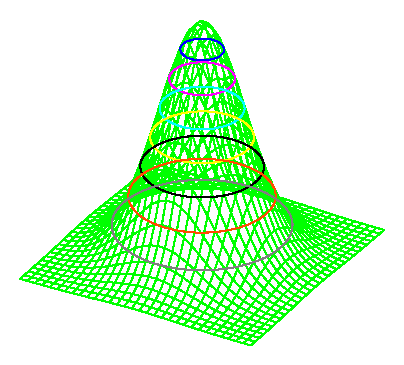
\includegraphics[width=\tw/4-15mm, height=\tw/4-15mm, clip=true]{../common/normxy_00.eps} &
  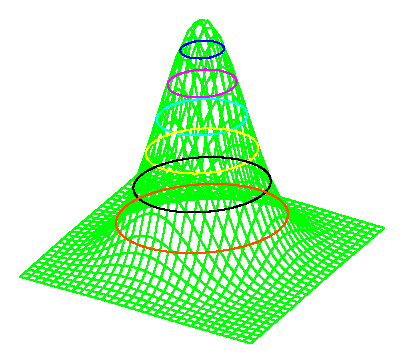
\includegraphics[width=\tw/4-15mm, height=\tw/4-15mm, clip=true]{../common/normxy_50.eps} &
  \includegraphics[width=\tw/4-15mm, height=\tw/4-15mm, clip=true]{../common/normxy_80.eps} & 
  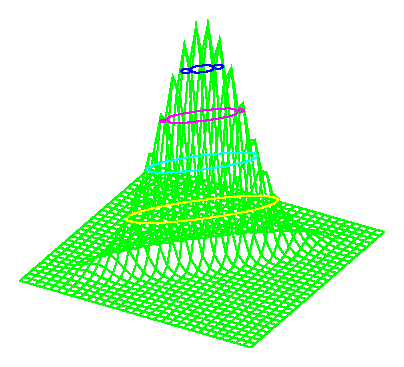
\includegraphics[width=\tw/4-15mm, height=\tw/4-15mm, clip=true]{../common/normxy_95.eps}
\end{tabular}
\caption{
  Joint Gaussian distributions $p(x,y)$ with varying correlations
  \label{fig:psub_joint_gaussian}
  %\citerp{moon2000}{35}
  }
\end{figure}

%=======================================
\section{Joint Gaussian distributions}
%=======================================
%---------------------------------------
\begin{definition}[Joint Gaussian pdf]
\citetbl{
  \citerp{proakis}{49}
  }
%---------------------------------------
\defbox{\begin{array}{rclD}
  \pp(x_1,x_2,\ldots,x_n) 
    &\eqd& \ds\frac{1}{\sqrt{(2\pi)^n |\vM|}}
           \exp{-\frac{1}{2}(\vx-\pE\vx)^T\vM^{-1}(\vx-\pE\vx)}
    &      (Gaussian joint pdf)
    \\ \\
  \vx 
    &\eqd& \left[\begin{array}{c}
             x_1    \\
             x_2    \\
             \vdots \\
             x_n
           \end{array}\right]
    \\
  \rvZ_k 
    &\eqd& X_k - \pE X_k
    & (zero mean random variables)
    \\ \\
  \vM 
    &\eqd& \brs{\begin{array}{cccc}
             \pE[\rvZ_1 \rvZ_1] & \pE[\rvZ_1 \rvZ_2] & \cdots & \pE[\rvZ_1 \rvZ_n]   \\
             \pE[\rvZ_2 \rvZ_1] & \pE[\rvZ_2 \rvZ_2] &        & \pE[\rvZ_2 \rvZ_n]   \\
             \vdots       & \vdots       & \ddots & \vdots         \\
             \pE[\rvZ_n \rvZ_1] & \pE[\rvZ_n \rvZ_2] & \cdots & \pE[\rvZ_n \rvZ_n]
           \end{array}}
    & (correlation matrix)
\end{array}}
\end{definition}


\begin{figure}[ht]
   \begin{center}
   \includegraphics[height=8cm, width=12cm, clip=]{../common/pdf_norm.eps} 
   \end{center}
\caption{
  Gaussian pdf with $\mu=0$ and $\sigma\in[0.1,2]$.
  \label{fig:net_norm}
}
\end{figure}


%---------------------------------------
\begin{lemma}[Leibniz integration rule]
%---------------------------------------
  \lembox{
    \deriv{}{x} \int_{\fa(x)}^{\fb(x)} \fg(t) \dt  
      = \fg(\fb(x))\fb'(x) - \fg(\fa(x))\fa'(x)
    }
\end{lemma}

%---------------------------------------
\begin{example}[1 variable joint Gaussian pdf]
%---------------------------------------
The \hid{Gaussian distribution} (or \hid{normal distribution} has pdf
\exbox{
  \ppx(x) \eqd \frac{1}{\sqrt{2\pi\sigma^2}}e^{\frac{-(x-\mu)^2}{2\sigma^2}}
  }

\begin{align*}
  t
    &= \arg_t \min_t 
       \brs{
       \frac{1}{2}\int_t^\infty    \frac{1}{\sqrt{2\pi\sigma^2}}e^{\frac{-(x-\mu)^2}{2\sigma^2}} +
       \frac{1}{2}\int_{-\infty}^t \frac{1}{\sqrt{2\pi\sigma^2}}e^{\frac{-(x-\eta)^2}{2\sigma^2}}
       }
  \\&= \arg_t \brb{\pderiv{}{t}
       \brs{
       \frac{1}{2}\int_t^\infty    \frac{1}{\sqrt{2\pi\sigma^2}}e^{\frac{-(x-\mu)^2}{2\sigma^2}} +
       \frac{1}{2}\int_{-\infty}^t \frac{1}{\sqrt{2\pi\sigma^2}}e^{\frac{-(x-\eta)^2}{2\sigma^2}}
       }=0}
  \\&= \arg_t \brb{\frac{1}{2\sqrt{2\pi\sigma^2}}
       \brs{
       \pderiv{}{t}\int_t^\infty    e^{\frac{-(x-\mu)^2}{2\sigma^2}} +
       \pderiv{}{t}\int_{-\infty}^t e^{\frac{-(x-\eta)^2}{2\sigma^2}}
       }=0}
  \\&= \arg_t \brb{
       \brs{
       \brp{e^{\frac{-(\infty-\mu)^2}{2\sigma^2}}0 - e^{\frac{-(t-\mu)^2}{2\sigma^2}}1} +
       \brp{e^{\frac{-(t-\mu)^2}{2\sigma^2}}1 - e^{\frac{-(\infty-\mu)^2}{2\sigma^2}}0}
       }=0}
  \\&= \arg_t \brb{
       \brs{e^{\frac{-(t-\eta)^2}{2\sigma^2}}- e^{\frac{-(t-\mu)^2}{2\sigma^2}}}=0}
  \\&= \arg_t \brb{(t-\eta)^2=(t-\mu)^2}
  \\&= \frac{\mu+\eta}{2}
\end{align*}
\end{example}

%---------------------------------------
\begin{example}[2 variable joint Gaussian pdf]
\label{prop:prob_gaussian_xy}
%---------------------------------------
\exbox{\begin{array}{rc>{\ds}l}
  z_1 &\eqd& x_1 - \pE x_1 \\
  z_2 &\eqd& x_2 - \pE x_2 \\
  \abs{M} &\eqd& \abs{\pE[z_1 z_1]\pE[z_2 z_2]-\pE[z_1 z_2]\pE[z_1 z_2]}
  \\ 
  \pp(x_1,x_2) &\eqd&
    \frac{1}{2\pi \sqrt{\abs{M}}}
    \exp\left(
      \frac{z_1^2\pE[z_2z_2] - 2z_1z_2\pE[z_1z_2] + z_2^2\pE[z_1z_1]}
            {-2\abs{M}}
        \right)
\end{array}}
\end{example}



  %============================================================================
% LaTeX File
% Daniel J. Greenhoe
%============================================================================
%======================================
\chapter{Statistics}
\label{chp:stats}
%======================================
%=======================================
\section{Expectation operator}
\index{expectation operator}
%=======================================
In a \structe{probability space} $\ps$, all probability information
is contained in the \fncte{measure} $\psp$ (or equivalently in the pdf or cdf
defined in terms of $\psp$).
Often times this information is overwhelming and a simpler statistic,
which does not offer so much information, is sufficient.
Some of the most common statistics can be conveniently expressed in terms
of the \hie{expectation operator} $\pE$.
%---------------------------------------
\begin{definition}
\label{def:pE}
%---------------------------------------
Let $\ps$ be a \structe{probability space} and
$\rvX$ a \fncte{random variable} on $\ps$ with
\fncte{probability density function} $\ppx$.
\defboxt{ 
  The \opd{expectation operator} $\pEx$ on $\rvX$ is defined as
  \\\indentx$\ds\pEx\rvX \eqd \int_{x\in\F} x \ppx(x) \dx$. 
}
\end{definition}

We already said that a \fncte{random variable} $\rvX$ is neither random nor a variable,
but is rather a function of an underlying process that does appear to be random.
However, because it is a function of a process that does appear random,
the \fncte{random variable} $\rvX$ also appears to be random.
That is, if we don't know the outcome of of the underlying experimental
process, then we also don't know for sure what $\rvX$ is, and so $\rvX$ does
indeed appear to be random.
However, eventhough $\rvX$ appears to be random,
the expected value $\pEx\rvX$  of $\rvX$ is {\bf not random}.
Rather it is a fixed value (like $0$ or $7.9$ or $-2.6$).

On the other hand, eventhough $\pE\rvX$ is {\bf not random},
note that $\pE(\rvX|\rvY)$ {\bf is random}.
This is because $\pE(\rvX|\rvY)$ is a function of $\rvY$.
That is, once we know that $\rvY$ equals some fixed value $y$
(like $0$ or $2.7$ or $-5.1$) then $\pE(\rvX|\rvY=y)$ is also fixed.
However, if we don't know the value of $\rvY$,
then $\rvY$ is still a \fncte{random variable} and the expression $\pE(\rvX|\rvY)$
is also random (a function of \fncte{random variable} $\rvY$).

Two common statistics that are conveniently expressed in terms of the
expectation operator are the \hie{mean} and \hie{variance}.
The mean is an indicator of the ``middle" of a probability distribution and the
variance is an indicator of the ``spread".
%---------------------------------------
\begin{definition}
\label{def:Mx}
\label{def:pvar}
\label{def:pVar}
\index{mean}
\index{variance}
%---------------------------------------
Let $\rvX$ be a \fncte{random variable} on the \structe{probability space} $\ps$.
The {\bf mean} $\pmeanx$ and {\bf variance} $\pVar(\rvX)$ of $\rvX$ are
\defbox{\begin{array}{FM>{\ds}rc>{\ds}l}
  (1).&The \fnctd{mean} $\pmeanx$ of $\rvX$ is 
    & \pmeanx  &\eqd& \pEx\rvX 
  \\
  (2).&The \fnctd{variance} $\pVar(\rvX)$ or $\pvarx$ of $\rvX$ is 
    & \pVar(\rvX) &\eqd& \pEx\left[(\rvX-\pEx\rvX)^2 \right]
\end{array}}
\end{definition}

The next theorem gives some useful relations for simple statistics.
%---------------------------------------
\begin{theorem}
\label{thm:pE}
%---------------------------------------
Let $\rvX$ be a \fncte{random variable} on the \structe{probability space} $\ps$.
\thmbox{\begin{array}{>{\ds}rc>{\ds}lCD}
    \pEx(a\rvX+b)    &=& \brp{a\pEx\rvX} + b       & \forall a,b\in\R & (\prope{linear})
  \\\pVar(a\rvX+b)   &=& a^2\pVar(\rvX)            & \forall a,b\in\R &
  \\\pVar(\rvX)      &=& \pEx(\rvX^2) - (\pEx\rvX)^2
\end{array}}
\end{theorem}
\begin{proof}
\begin{align*}
  \pEx(a\rvX+b)
    &\eqd \int_{x\in\R}\brs{ax+b} \ppx(x)  \dx
  \\&=    a \int_{x\in\R}x \ppx(x)  \dx + b\int_{x\in\R}\ppx(x)  \dx
  \\&= \brs{a\pEx\rvX} + b\brs{1}
  \\&= \brs{a\pEx\rvX} + b
\\
\\
  \pVar(\rvX)
    &\eqd \pEx\left[(\rvX-\pEx\rvX)^2\right]
    &&    \text{by definition of $\pVar$}
    &&    \text{\xref{def:pvar}}
  \\&=    \pEx\brs{\rvX^2-2X\pEx\rvX + (\pEx\rvX)^2 }
  \\&=    \pEx[\rvX^2]  - \pEx 2X\pEx\rvX  + \pEx (\pEx\rvX)^2
  \\&=    \pEx[\rvX^2] - 2(\pEx\rvX)[\pEx\rvX] + (\pEx\rvX)^2
  \\&=    \pEx(\rvX^2) - (\pEx\rvX)^2
\\
\\
  \pVar(a\rvX+b)
    &=    \pEx(a\rvX+b)^2  - [\pEx(a\rvX+b)]^2
  \\&=    \pEx(a^2X^2+2ab\rvX+b^2)  - [a(\pEx\rvX)+b]^2
  \\&=    a^2 \pEx\rvX^2  +2ab\pEx\rvX + b^2 - \brs{a^2[\pEx\rvX]^2 + 2ab\pEx\rvX + b^2}
  \\&=    a^2\brs{ \pEx\rvX^2  - (\pEx\rvX)^2 }
  \\&\eqd a^2 \pVar(\rvX)
\end{align*}
\end{proof}

\begin{figure}[ht]
\setlength{\unitlength}{0.3mm}%
\begin{center}%
\begin{picture}(200,110)(-50,-10)%
  \thicklines
  \color{axis}%
    \put(  0,  0){\line(1, 0){120}}%
    \put(  0,  0){\line(0, 1){100}}%
    \qbezier[20](0,60)(30,60)(60,60)%
    \qbezier[20](60,0)(60,30)(60,60)%
  \color{blue}%
    \qbezier(33,100)(85,0)(110,100)%
    \put( 60, 60){\circle*{5}}%
  \color{red}%
    \put( 20,100){\line(1,-1){80}}%
  \color{label}%
  \put(125,  0){\makebox(0,0)[l]{$x$}}%
  \put( -5, 60){\makebox(0,0)[r]{$\ff(\pE\rvX)$}}%
  \put( 60, -5){\makebox(0,0)[t]{$\pE\rvX$}}%
  \put(130,60){\vector(-1,0){32}}%
  \put(130,40){\vector(-1,0){47}}%
  \put(135,60){\makebox(0,0)[l]{$\ff(x)$ (convex function)}}%
  \put(135,40){\makebox(0,0)[l]{$mx+c$ (support line)}}%
\end{picture}
\end{center}
\caption{
  Jensen's inequality
  \label{fig:jensen}
  }
\end{figure}

\fncte{Jensen's inequality} is an extremely useful application of \prope{convex}ity \xref{def:convex} to the
\ope{expectation} operator.
Jensen's inequality is stated in \pref{cor:jensen} (next)
and illustrated in \prefpp{fig:jensen}.
%--------------------------------------
\begin{corollary}[\thmd{Jensen's inequality}]
\footnote{
  \citerp{cover}{25},
  \citerpp{jensen1906}{179}{180}
  }
\label{cor:jensen}
%--------------------------------------
Let $\ff$ be a function in $\clFrr$ and $\rvX$ be a \fncte{random variable} on $\ps$.
\corbox{
  \brb{\text{$\ff$ is \prope{convex}}} 
  \quad\implies\quad 
  \brb{\ff(\pE\rvX) \le \pE\ff(\rvX)}
  }
\end{corollary}
\begin{proof}
\begin{enumerate}
  \item Proof 1:
Let $mx+c$ be a ``support line" under $\ff(x)$ \xref{fig:jensen} such that
\[
  \begin{array}{rcll}
    mx+c &<& \ff(x) & \mbox{for } x\ne \pE\rvX \\
    mx+c &=& \ff(x) & \mbox{for } x=\pE\rvX.
  \end{array}
\]
Then
\begin{align*}
  \ff(\pE\rvX)
    &=   m[\pE\rvX] + c
  \\&=   \pE[mX + c]
  \\&\le \pE\ff(\rvX)
\end{align*}

  \item Proof 2 (alternate proof):
    \begin{align*}
      \ff\brp{\pE\rvX}
        &\eqd \ff\brp{\sum_{x\in\pse} x \psp(x)}
      \\&\le \sum_{x\in\pse} \ff(x) \psp(x)
        && \text{by \thme{Jensen's inequality} for convex sets}
        && \text{\xref{thm:jensenineq}}
    \end{align*}
\end{enumerate}
\end{proof}

%=======================================
\section{Upper bounds on probability}
%=======================================
%---------------------------------------
\begin{theorem}[\thmd{Markov's inequality}]
\citetbl{
  \citerp{ross}{395}
  }
\label{thm:markovineq}
%---------------------------------------
Let $\rvX:\Omega\to[0,\infty)$ be a non-negative valued \fncte{random variable} and
$a\in(0,\infty)$. Then
\thmbox{ \psp\setn{\rvX\ge a} \le \frac{1}{a} \pE\rvX }
\end{theorem}
\begin{proof}
\begin{align*}
  I &\eqd \left\{ \begin{array}{l@{\hspace{4ex}\mbox{for}\hspace{4ex}}l}
    1 &\rvX\ge a \\
    0 &\rvX < a
    \end{array}\right.
\\
  aI &\le\rvX           \\
   I &\le \frac{1}{a}\rvX \\
   \pE I &\le \pE\left(\frac{1}{a}\rvX\right) \\
\\
   \psp\setn{\rvX\ge a}
     &= 1\cdot\psp\setn{\rvX\ge a} + 0\cdot\psp\setn{\rvX<a}
   \\&= \pE I
   \\&\le \pE\left(\frac{1}{a}\rvX \right)
   \\&=   \frac{1}{a}\pE\rvX
\end{align*}
\end{proof}


%---------------------------------------
\begin{theorem}[Chebyshev's inequality]
\index{Chebyshev's inequality}
\index{theorems!Chebyshev's inequality}
\citetbl{
  \citerp{ross}{396}
  }
%---------------------------------------
Let $\rvX$ be a \fncte{random variable} with mean $\mu$ and variance $\sigma^2$.
\thmbox{ \psp\setn{\abs{\rvX-\mu}\ge a} \le \frac{\sigma^2}{a^2}}
\end{theorem}
\begin{proof}
\begin{align*}
  \psp\setn{\abs{\rvX-\mu} \ge a}
    &=   \psp\setn{ (\rvX-\mu)^2 \ge a^2}
  \\&\le \frac{1}{a^2} \pE(\rvX-\mu)^2 
    && \text{by \thme{Markov's inequality}}
    && \text{\xref{thm:markovineq}}
  \\&=   \frac{\sigma^2}{a^2}
\end{align*}
\end{proof}

%=======================================
\section{Joint and conditional probability spaces}
%=======================================
Sometimes the problem of finding the expected value of a \fncte{random variable} $\rvX$
can be simplified by ``conditioning $\rvX$ on $\rvY$".
%---------------------------------------
\begin{theorem}
%---------------------------------------
Let $\rvX$ and $\rvY$ be \fncte{random variable}s. Then
\thmbox{\pEx{\rvX} = \pEy\pEx[x|y](\rvX|\rvY) }
\end{theorem}
\begin{proof}
\begin{align*}
   \pEy\pEx[x|y](\rvX|\rvY)
     &\eqd \pEy \left[ \int_{x\in\R}x \pp(\rvX=x|\rvY) \dx \right]
   \\&\eqd \int_{y\in\R} \left[\int_{x\in\R}x \pp(x|\rvY=y) \dx \right] \pp(y) \dy
   \\&=    \int_{y\in\R} \int_{x\in\R}x \pp(x|y)\pp(y) \dx   \dy
   \\&=    \int_{x\in\R}x \int_{y\in\R} \pp(x,y) \dy   \dx
   \\&=    \int_{x\in\R}x \pp(x) \dx
   \\&\eqd \pEx\rvX
\end{align*}
\end{proof}

When possible, we like to generalize any given mathematical structure
to a more general mathematical structure and then take advantage of
the properties of that more general structure.
Such a generalization can be done with \fncte{random variable}s.
Random variables can be viewed as vectors in a vector space.
Furthermore, the expectation of the product of two \fncte{random variable}s
(e.g. $\pE(\rvX\rvY)$)
can be viewed as an \fncte{inner product} in an \structe{inner product space}.
Since we have an \fncte{inner product} space,
we can then immediately use all the properties of
\structe{inner product space}s, \fncte{norm}ed spaces, vector spaces, metric spaces,
and topological spaces.

%---------------------------------------
\begin{theorem}
\citetbl{
  \citerpp{moon2000}{105}{106}
  }
\label{thm:prb_vspace}
%---------------------------------------
Let $R$ be a ring,
$\ps$ be a \structe{probability space}, $\pE$ the expectation operator, and
$\spV=\set{\rvX}{\rvX:\pso\to R}$ be the set of all random vectors
in \structe{probability space} $\ps$.
\thmbox{\begin{array}{FlM}
  (1). & \spV\eqd\set{\rvX}{\rvX:\pso\to R}        & is a \structe{vector space}. \\
  (2). & \inprod{\rvX}{\rvY}\eqd\pE(\rvX\rvY^\ast) & is an \fncte{inner product}. \\
  (3). & \norm{\rvX}\eqd\sqrt{\pE(\rvX\rvX^\ast)}  & is a \fncte{norm}. \\
  (4). & \opair{\spV}{\inprodn}                    & is an \structe{inner product space}.
\end{array}}
\end{theorem}
\begin{proof}
\begin{enumerate}
  \item Proof that $\spV$ is a vector space:
    \[\begin{array}{lll@{\hs{1cm}}D}
   1) & \forall \rvX,\rvY, \rvZ\in\spV
      & (\rvX+\rvY)+ \rvZ = \rvX+(\rvY+ \rvZ)
      & \text{($+$ is associative)}
      \\
   2) & \forall \rvX,\rvY\in\spV
      & \rvX+\rvY = \rvY+\rvX
      & \text{($+$ is commutative)}
      \\
   3) & \exists  0 \in\spV \st \forall \rvX\in\spV
      & \rvX+ 0 = \rvX
      & \text{($+$ identity)}
      \\
   4) & \forall \rvX \in\spV \exists \rvY\in\spV \st
      & \rvX+\rvY =  0
      & \text{($+$ inverse)}
      \\
   5) & \forall \alpha\in S \text{ and } \rvX,\rvY\in\spV
      & \alpha\cdot(\rvX+\rvY) = (\alpha \cdot\rvX)+(\alpha\cdot\rvY)
      & \text{($\cdot$ distributes over $+$)}
      \\
   6) & \forall \alpha,\beta\in S \text{ and } \rvX\in\spV
      & (\alpha+\beta)\cdot\rvX = (\alpha\cdot \rvX)+(\beta\cdot \rvX)
      & \text{($\cdot$ pseudo-distributes over $+$)}
      \\
   7) & \forall \alpha,\beta\in S \text{ and } \rvX\in\spV
      & \alpha(\beta\cdot\rvX) = (\alpha\cdot\beta)\cdot\rvX
      & \text{($\cdot$ associates with $\cdot$)}
      \\
   8) & \forall \rvX\in\spV
      & 1\cdot \rvX = \rvX
      & \text{($\cdot$ identity)}
\end{array}\]

  \item Proof that $\inprod{\rvX}{\rvY}\eqd\pE(\rvX\rvY^\ast)$ is an \fncte{inner product}.
  \[\begin{array}{llllD}
   1) &  \pE(\rvX\rvX^\ast) &\ge 0
      &  \forall \rvX\in\spV
      &  \text{(non-negative)}
      \\
   2) &  \pE(\rvX\rvX^\ast) &= 0 \iff \rvX=0
      &  \forall \rvX\in\spV
      &  \text{(non-degenerate)}
      \\
   3) &  \pE(\alpha\rvX\rvY^\ast)    &= \alpha\pE(\rvX\rvY^\ast)
      &  \forall \rvX,\rvY\in\spV,\;\forall\alpha\in\C
      &  \text{(homogeneous)}
      \\
   4) &  \pE[(\rvX+\rvY)\rvZ^\ast] &= \pE(\rvX\rvZ^\ast) + \pE(Y\rvZ^\ast)
      &  \forall \rvX,\rvY, \rvZ\in\spV
      &  \text{(additive)}
      \\
   5) &  \pE(\rvX\rvY^\ast) &= \pE(\rvY\rvX^\ast)
      &  \forall \rvX,\rvY\in\spV
      &  \text{(conjugate symmetric)}.
  \end{array}\]

  \item Proof that $\norm{\rvX}\eqd\sqrt{\pE(\rvX\rvX^\ast)}$ is a \fncte{norm}:
    This \fncte{norm} is simply induced by the above \fncte{inner product}.
  \item Proof that $\opair{\spV}{\inprodn}$ is an \structe{inner product space}:
    Because $\spV$ is a vector space and $\inprodn$ is
    an \fncte{inner product}, $\opair{\spV}{\inprodn}$ is an \structe{inner product space}.
\end{enumerate}
\end{proof}

The next theorem gives some results that follow directly from vector space
properties:
%---------------------------------------
\begin{theorem}
%---------------------------------------
Let $\ps$ be a \structe{probability space} with expectation functional $\pE$.
\thmbox{\begin{array}{l >{\ds}r c >{\ds}l D}
  1. & \sqrt{\pE\left(\sum_{n=1}^{\xN}\rvX_n\right)}
     &\le& \sum_{n=1}^{\xN} \pE(\rvX_nX_n^\ast)
     & (\thme{Generalized triangle inequality})
     \\
  2. & \abs{\pE(\rvX\rvY^\ast)}^2
     &\le& \pE(\rvX\rvX^\ast)\:\pE(YY^\ast)
     & (\thme{Cauchy-Schwartz inequality})
     \\
  3. & 2\pE(\rvX\rvX^\ast) + 2\pE(YY^\ast)
     &=& \pE[(\rvX+\rvY)(\rvX+\rvY)^\ast] + \pE[(\rvX-Y)(\rvX-Y)^\ast]
     &   (\thme{Parallelogram Law})
  \end{array}}
\end{theorem}
\begin{proof}
\begin{enumerate}
  \item $\opair{\clFor}{\pE(\rvx,\rvy)}$ is an \structe{inner product space}. Proof: \prefpp{thm:prb_vspace}.

  \item Because it is an \structe{inner product space}, the other properties follow:
        \\\indentx\begin{tabular}{llll}
          1. & Generalized triangle inequality:
             & \pref{thm:norm_tri}
             & \prefpo{thm:norm_tri}
             \\
          2. & Cauchy-Schwartz inequality:
             & \pref{thm:cs}
             & \prefpo{thm:cs}
             \\
          3. & Parallelogram Law:
             & \pref{thm:parallelogram}
             & \prefpo{thm:parallelogram}
        \end{tabular}
\end{enumerate}
\end{proof}


  %============================================================================
% LaTeX File
% Daniel J. Greenhoe
%============================================================================

%======================================
\chapter{Random Processes}
\label{app:random_processes}
%======================================
\qboxnps
  {Aristotle (384 BC -- 322 BC)
    \index{Aristotle}
    \index{quotes!Aristotle}
    \footnotemark
  }
  {../common/people/aristot.jpg}
  {A likely impossibility is always preferable to an
  unconvincing possibility.}
  \footnotetext{\begin{tabular}[t]{ll}
    quote: & \url{http://en.wikiquote.org/wiki/Aristotle} \\
    image: & \url{http://en.wikipedia.org/wiki/Aristotle}
  \end{tabular}}



%=======================================
\section{Continuous-time random processes}
%=======================================
%=======================================
\subsection{Definitions}
%=======================================
%---------------------------------------
\begin{definition}
\index{random variable}
\index{random process}
\citetbl{
  \citerp{papoulis}{63},
  \citerp{papoulis}{285}
  }
%---------------------------------------
Let $\ps$ be a \structe{probability space}.\\
\defboxt{
  The function $\rvx:\pso\to\R$ is a \fnctd{random variable}.\\
  The function $\rvy:\R\times\pso\to\R$ is a \fnctd{random process}.
  }
\end{definition}

The random process $\rvx(t,\omega)$, where $t$ commonly represents time
and $\omega\in\pso$ is an outcome of an experiment,
can take on more specialized forms depending on whether
$t$ and $\omega$ are fixed or allowed to vary.
These forms are illustrated in \prefp{fig:X(t,w)}\footnote{\citerpp{papoulis}{285}{286}}
and \prefp{fig:X(t,w)graph}.

\begin{figure}[ht]\color{figcolor}
\begin{center}
   \begin{tabular}{|c||c|c|}
      \hline
         $\rvx(t,\omega)$ &  fixed $t$      & variable $t$   \\
      \hline
      \hline
         fixed    $\omega$ & number          & time function  \\
      \hline
         variable $\omega$ & random variable & random process \\
      \hline
   \end{tabular}
\caption{
   Specialized forms of a random process $\rvx(t,\omega)$
   \label{fig:X(t,w)}
   }
\end{center}
\end{figure}

\begin{figure}[ht]\color{figcolor}
\begin{center}
\includegraphics[height=8cm,width=12cm]{../common/x_tw.eps}
\end{center}
\caption{
  Example of a random process $\rvx(t,\omega)$
  \label{fig:X(t,w)graph}
}
\end{figure}


%---------------------------------------
\begin{definition}
%\label{def:Mx}
\index{mean}
\label{def:Rxx}
\label{def:opR}
\index{auto-correlation }
\index{correlation!auto-correlation }
\label{def:Rxy}
\index{cross-correlation }
\index{correlation!cross-correlation }
\index{Fredholm integral equation of the first kind}
%---------------------------------------
Let $x(t)$ and $y(t)$ be random processes.
Then

\begin{tabular}{cll}
   $\imark$ & $\Mx(t):X\to\R$       & is the \textbf{mean} of $x(t)$                          \\
   $\imark$ & $\Rxy:X\times X\to\R$ & is the \textbf{crosscorrelation} of $x(t)$ and $y(t)$   \\
   $\imark$ & $\Rxx:X\to\R$         & is the \textbf{autocorrelation function} of $x(t)$      \\
   $\imark$ & $\opR:\vCc\to\vCc$    & is the \textbf{autocorrelation operator}
\end{tabular}

such that
\footnote{
   The equation $\int_u \Rxx(t,u) f(u) \du$ is a
   \textbf{Fredholm integral equation of the first kind} and
   $\Rxx(t,u)$ is the \textbf{kernel} of the equation.
   References: 
     \citer{fredholm1900},
     \citerp{fredholm1903}{page 365},
     \citerp{michel1993}{page 97},
     \citerp{keener}{page 101}
   }
\defbox{\begin{array}{rc>{\ds}ll}
   \Mx(t)    &\eqd& \pEb{\rvx(t)}             & \text{(mean functional)} \\
   \Rxy(t,u) &\eqd& \pEb{\rvx(t)\rvy^\ast(u)} & \text{(cross-correlation bilinear functional)} \\
   \Rxx(t,u) &\eqd& \pEb{\rvx(t)\rvx^\ast(u)} & \text{(auto-correlation bilinear functional)} \\
   \opR f    &\eqd& \int_u \Rxx(t,u) f(u) \du & \text{(auto-correlation operator)}
\end{array}}
\end{definition}



%---------------------------------------
\subsection{Properties}
%---------------------------------------

%---------------------------------------
\begin{theorem}
\label{thm:Rxx_prop}
\index{cross-correlation}
\index{symmetric!conjugate}
\index{conjuage symmetric}
%---------------------------------------
Let $\fx(t)$ and $\fy(t)$ be random processes with
cross-correlation $\Rxy(t,u)$ and
let $\Rxx(t,u)$ be the auto-correlation of $\fx(t)$.
\thmbox{
\begin{array}{rcll}
   \Rxx(t,u) &=& \Rxx^\ast(u,t) & \text{(conjugate symmetric)}\\
   \Rxy(t,u) &=& \Ryx^\ast(u,t) & \text{(conjugate symmetric)}.
\end{array}
}
\end{theorem}

\begin{proof}
\[\begin{array}{*{12}{l}}
   \Rxx(t,u)
      &\eqd& \E[\rvx(t) \rvx^\ast(u)]
      &=&      \E[\rvx^\ast(u) \rvx(t) ]
      &=&      \left( \E[\rvx(u) \rvx^\ast(t) ] \right)^\ast
      &\eqd& \Rxx^\ast(u,t)
\\
   \Rxy(t,u)
      &\eqd& \E[\rvx(t) \rvy^\ast(u)]
      &=&      \E[\rvy^\ast(u) \rvx(t) ]
      &=&      \left( \E[\rvy(u) \rvx^\ast(t) ] \right)^\ast
      &\eqd& \Ryx^\ast(u,t)
\end{array}\]
\end{proof}


%---------------------------------------
\begin{theorem}
\index{non-negative}
\index{positive definite}
%---------------------------------------
Let $\opR:\spX\to\spX$ be an auto-correlation operator.
\thmbox{\begin{array}{ll@{\qquad}l}
  \inprod{\opR \fx}{\fx} \ge 0
    & \forall \fx\in\spX
    & \text{(non-negative)}  \\
  \inprod{\opR \fx}{\fy} = \inprod{\fx}{\opR \fy}
    & \forall \fx,\fy\in\spX
    & \text{(self-adjoint)}
\end{array}}
\end{theorem}
\begin{proof}
\begin{align*}
\intertext{1. Proof that $\opR$ is non-negative:}
   \inprod{\opR \fy}{\fy}
     &= \inprod{\int_u \Rxx(t,u) \fy(u) \du}{\fy(t)}
     && \text{by definition of $\opR$ (\prefp{def:opR})}
   \\&= \inprod{\int_u \Eb{\fx(t)\fx^\ast(u)} \fy(u) \du}{\fy(t)}
     && \text{by definition of $\Rxx$ (\prefp{def:Rxx})}
   \\&= \pEb{\inprod{\int_u \fx(t)\fx^\ast(u) \fy(u) \du}{\fy(t)}}
     && \text{by linearity of funtional $\inprodn$ and operator $\int$}
   \\&= \pEb{\int_u \fx^\ast(u) \fy(u) \du \inprod{\fx(t)}{\fy(t)}}
     && \text{by \prope{additivity} property of $\inprodn$\ifsxref{vsinprod}{def:inprod}}
   \\&= \pEb{\inprod{\fy(u)}{\fx(u)} \inprod{\fx(t) }{\fy(t)}}
     && \text{by local definition of $\inprodn$}
   \\&= \pEb{\inprod{\fx(u)}{\fy(u)}^\ast \inprod{\fx(t) }{\fy(t)}}
     && \text{by \prope{conjugate symmetry} property of $\inprodn$\ifsxref{vsinprod}{def:inprod}}
   \\&= \pE{\left| \inprod{\fx(t) }{\fy(t)} \right|^2}
     && \text{by definition of $\absn$} %(\prefp{def:abs})
   \\&\ge 0
\intertext{2. Proof that $\opR$ is self-adjoint:}
   \inprod{\brs{\opR \fx}(t)}{\fy}
     &= \inprod{\int_u \Rxx(t,u) \fx(u) \du}{\fy(t)}
     && \text{by definition of $\opR$ (\prefp{def:opR})}
   \\&= \int_u \fx(u) \inprod{\Rxx(t,u)  }{\fy(t)} \du
     && \text{by \prope{additivity} property of $\inprodn$\ifsxref{vsinprod}{def:inprod}}
   \\&= \int_u \fx(u) \inprod{\fy(t)}{\Rxx(t,u)}^\ast \du
     && \text{by \prope{conjugate symmetry} property of $\inprodn$\ifsxref{vsinprod}{def:inprod}}
   \\&= \inprod{ \fx(u) }{\inprod{\fy(t)}{\Rxx(t,u)} }
     && \text{by local definition of $\inprodn$}
   \\&= \inprod{ \fx(u) }{\int_t \fy(t) \Rxx^\ast(t,u)\dt }
     && \text{by local definition of $\inprodn$}
   \\&= \inprod{ \fx(u) }{\int_t \fy(t) \Rxx(u,t)\dt }
     && \text{by \prefp{thm:Rxx_prop}}
   \\&= \inprod{ \fx(u) }{\mcom{\opR}{$\opRa$} \fy }
     && \text{by definition of $\opR$ (\prefp{def:opR})}
   \\\implies&\qquad \opR=\opRa \qquad\implies \text{$\opR$ is self adjoint}
\end{align*}
\end{proof}


%---------------------------------------
\begin{theorem}
\index{autocorrelation}
\index{symmetric!conjugate}
\index{conjugate symmetric}
\index{non-negative definite}
\index{positive definite}
\index{self-adjoint}
\index{kernel}
\index{orthogonal}
%---------------------------------------
Let $\seq{\lambda_n}{n\in\Z}$ be the eigenvalues and
    $\seq{\fpsi_n}{n\in\Z}$ be the eigenfunctions of
    operator $\opR$ such that
    $\opR \psi_n = \lambda_n \psi_n$.
\thmbox{\begin{array}{rlp{7cm}}
  1. & \lambda_n \in \R
     & (eigenvalues of $\opR$ are real)
     \\
  2. & \lambda_n\ne \lambda_m \implies \inprod{\psi_n}{\psi_m}=0
     & (eigenfunctions associated with distinct eigenvalues are orthogonal)
     \\
  3. & \norm{\psi_n(t)}^2>0 \implies \lambda_n\ge0
     & (eigenvalues are non-negative)
     \\
  4. & \norm{\psi_n(t)}^2>0, \inprod{\opR f}{f} > 0 \implies \lambda_n>0
     & (if $\opR$ is positive definite, then eigenvalues are positive)
     \\
  5. & \E{\left| x(t)-\sum_n \inprod{x(t)}{\psi_n(t)} \psi_n(t) \right|^2} = 0
     & ($\{\psi_n(t)\}$ is a basis for $x(t)$)
\end{array}}
\end{theorem}
\begin{proof}
\begin{enumerate}
\item Eigenvalues are real:
Because $\opR$ is self-adjoint, its eigenvalues are real\ifsxref{operator}{thm:self_adjoint}.

\item eigenfunctions associated with distinct eigenvalues are orthogonal:
Because $\opR$ is self-adjoint, this property follows\ifsxref{operator}{thm:self_adjoint}.

\item Eigenvalues are non-negative:
\begin{align*}
   0 &\ge \inprod{\opR \psi_n}{\psi_n}
     &&   \text{by definition of non-negative definite}
   \\&=   \inprod{\lambda_n \psi_n}{\psi_n}
     &&   \text{by hypothesis}
   \\&=   \lambda_n \inprod{\psi_n}{\psi_n}
     &&   \text{by definition of inner-products}
   \\&=   \lambda_n \norm{\psi_n}^2
     &&   \text{by definition of norm induced by inner-product}
\end{align*}

\item Eigenvalues are positive if $\opR$ is positive definite:
\begin{align*}
   0 &> \inprod{\opR \psi_n}{\psi_n}
     && \text{by definition of positive definite}
   \\&= \inprod{\lambda_n \psi_n}{\psi_n}
     && \text{by hypothesis}
   \\&= \lambda_n \inprod{\psi_n}{\psi_n}
     && \text{by definition of inner-products}
   \\&= \lambda_n \norm{\psi_n}^2
     && \text{by definition of norm induced by inner-product}
\end{align*}

\item $\{\psi_n(t)\}$ is a basis for $x(t)$
      \[ \E{\left| x(t)-\sum_n \dot{x}_n \psi_n(t) \right|^2} = 0
         \hspace{1cm}\mbox{where } \dot{x}_n\eqd \inprod{x(t)}{\psi_n(t)}
      \]

\begin{eqnarray*}
   \Eb{x(t) \left(\sum_n \dot{x}_n \psi_n(t)\right)^\ast}
     &=& \Eb{x(t) \left(\sum_n \int_u x(u)\psi_n^\ast(u)\du \psi_n(t)\right)^\ast}
   \\&=&  \sum_n \left(\int_u \Eb{x(t)x^\ast(u)}\psi_n(u)\du\right) \psi_n^\ast(t)
   \\&=&  \sum_n \left(\int_u \Rxx(t,u)\psi_n(u)\du\right) \psi_n^\ast(t)
   \\&=&  \sum_n \lambda_n\psi_n(t) \psi_n^\ast(t)
   \\&=&  \sum_n \lambda_n \left|\psi_n(t) \right|^2
\\ \\
   \Eb{\sum_n \dot{x}_n \psi_n(t)\left(\sum_m \dot{x}_m \psi_m(t)\right)^\ast}
     &=& \Eb{\sum_n \int_u x(u)\psi_n^\ast(u)\du   \psi_n(t)\left(\sum_m \int_v x(v)\psi_m^\ast(v)\dv \psi_m(t)\right)^\ast}
   \\&=& \sum_n\sum_m \int_u\left(\int_v \Eb{x(u)x^\ast(v)}\psi_m(v)\dv\right) \psi_n^\ast(u)\du   \psi_n(t)   \psi_m^\ast(t)
   \\&=& \sum_n\sum_m \int_u\left(\int_v \Rxx(u,v)\psi_m(v)\dv\right) \psi_n^\ast(u)\du   \psi_n(t)   \psi_m^\ast(t)
   \\&=& \sum_n\sum_m \int_u\left(\lambda_m\psi_m(u)\right) \psi_n^\ast(u)\du   \psi_n(t)   \psi_m^\ast(t)
   \\&=& \sum_n\sum_m \lambda_m \left(\int_u \psi_m(u) \psi_n^\ast(u)\du \right)   \psi_n(t)   \psi_m^\ast(t)
   \\&=& \sum_n\sum_m \lambda_m \kdelta_{mn}   \psi_n(t)   \psi_m^\ast(t)
   \\&=& \sum_n \lambda_n   \psi_n(t)   \psi_n^\ast(t)
   \\&=& \sum_n \lambda_n  \left| \psi_n(t) \right|^2
\end{eqnarray*}


Using these two results, we can prove the following:

\begin{eqnarray*}
  &&\E{\left| x(t)-\sum_n \dot{x}_n \psi_n(t) \right|^2}
  \\&=& \Eb{\left[ x(t)-\sum_n \dot{x}_n \psi_n(t) \right]\left[ x(t)-\sum_m \dot{x}_m \psi_m(t) \right]^\ast}
  \\&=& \Eb{x(t)x^\ast(t) -x(t)\left(\sum_n \dot{x}_n \psi_n(t)\right)^\ast -x^\ast(t)\sum_n \dot{x}_n \psi_n(t) + \sum_n \dot{x}_n \psi_n(t) \left(\sum_m \dot{x}_m \psi_m(t) \right)^\ast }
  \\&=& \Eb{x(t)x^\ast(t)} -\Eb{x(t)\left(\sum_n \dot{x}_n \psi_n(t)\right)^\ast} -\Eb{x^\ast(t)\sum_n \dot{x}_n \psi_n(t)} + \Eb{\sum_n \dot{x}_n \psi_n(t) \left(\sum_m \dot{x}_m \psi_m(t) \right)^\ast }
  \\&&  \text{by \prop{Mercer's Theorem}\ifsxref{integrat}{thm:mercer}}
  \\&=& \sum_n \lambda_n |\psi_n(t)|^2 -\sum_n \lambda_n \left|\psi_n(t) \right|^2  -\left(\sum_n \lambda_n \left|\psi_n(t) \right|^2\right)^\ast + \sum_n \lambda_n \left|\psi_n(t) \right|^2
  \\&=& \sum_n \lambda_n |\psi_n(t)|^2 -\sum_n \lambda_n \left|\psi_n(t) \right|^2  -\sum_n \lambda_n \left|\psi_n(t) \right|^2 + \sum_n \lambda_n \left|\psi_n(t) \right|^2
  \\&=& 0
\end{eqnarray*}
\end{enumerate}
Reference: \citerpp{keener}{114}{119}
\end{proof}

%=======================================
\subsection{Karhunen-Lo\`{e}ve Expansion}
\label{sec:KL}
\index{Karhunen-Lo\`{e}ve Expansion}
\index{eigenfunctions}
\index{eigenvalues}
%=======================================
If a random process $x(t)$ is white
\footnote{{\em white noise process}: random process $x(t)$ with autocorrelation $\Rxx(\tau)=\delta(\tau)$}
and $\Psi=\{\psi_1(t),\psi_2(t),\ldots,\psi_N(t)\}$ is \textbf{any} set of orthonormal basis functions,
then the innerproducts
$\inprod{n(t)}{\psi_n(t)}$ and $\inprod{n(t)}{\psi_m(t)}$ are uncorrelated
for $m\ne  n$.
However, if $x(t)$ is colored (not white), then the innerproducts are not
in general uncorrelated.
But if the elements of $\Psi$ are chosen to be the eigenfunctions of $\opR$ such
that
\[ \opR \psi_n = \lambda_n \psi_n,\]
then by \prefp{thm:Rxx_prop}, $\{\psi_n(t)\}$ are orthogonal and
the innerproducts \textbf{are} uncorrelated eventhough $x(t)$ is
not white.
This criterion is called the  Karhunen-Lo\`{e}ve criterion for $x(t)$.




%=======================================
\subsection{LTI Operations on non-stationary random processes}
\index{LTI!operations on non-stationary random processes}
%=======================================
\begin{figure}[ht]\color{figcolor}
\begin{fsK}
\begin{center}
  \setlength{\unitlength}{0.2mm}
  \begin{picture}(300,130)(-100,-80)
  \thinlines
  %\graphpaper[10](0,0)(160,80)
  \put(-100,  10 ){\makebox (100, 40)[b]{$\rvx(t)$}  }
  \put(-100, -50 ){\makebox (100, 40)[t]{$\Rxx(t,u)$}  }
  \put(-100,   0 ){\vector  (  1,  0){100}             }
  \put(   0, -50 ){\framebox(100,100){$\conv \fh(t)$}  }
  \put( 100,   0 ){\vector  (  1,  0){100}             }
  \put( 110,  10 ){\makebox (100, 40)[lb]{$\ds\rvy(t)=\rvx(t)\conv\fh(t)=\int_u\fh(u)\rvx(t-u)\du$}  }
  \put( 100, -50 ){\makebox (100, 40)[t]{$\Ryy(t,u)$}  }
  \put(  50, -60 ){\makebox (  0,  0)[t]{$\Rxy(t,u)$}  }
  \end{picture}
\caption{
   Linear system with random process input and output
   \label{fig:linear-sys}
   }
\end{center}
\end{fsK}
\end{figure}

%---------------------------------------
\begin{theorem}
\index{linear time invariant}
\footnote{\citerp{papoulis}{312}}
%---------------------------------------
Let $h:\R\to\C$ be the impulse response of a linear time-invariant system and
Let $\rvy(t)=h(t)\conv \rvx(t) \eqd \int_u h(u)\rvx(t-u) \du$ as
illustrated in \prefp{fig:linear-sys}.
Then
\thmbox{\begin{array}{rclcl}
\mc{5}{l}{\mbox{\bf Correlation functions}} \\
   \Rxy(t,u)
     &=&    \Rxx(t,u) \conv h^\ast(u)
     &\eqd& \int_v \fh^\ast(v)  \Rxx(t,u-v)  \dv
\\
   \Ryy(t,u)
     &=&    \Rxy(t,u) \conv \fh(t)
     &\eqd& \int_v \fh(v) \Rxy(t-v,u) \dv
\\
   \Ryy(t,u)
     &=&    \Rxx(t,u) \conv \fh(t) \conv \fh^\ast(u)
     &\eqd& \int_w \fh^\ast(w) \int_v \fh(v) \Rxx(t-v,u-w) \dv\dw
\\ \\
\mc{5}{l}{\mbox{\bf Laplace power spectral density functions}} \\
   \LSxy(s,r) &=& \LSxx(s,r) \Lh^\ast(r^\ast)         \\
   \LSyy(s,r) &=& \LSxy(s,r) \Lh(s)              \\
   \LSyy(s,r) &=& \LSxx(s,r) \Lh(s) \Lh^\ast(r^\ast)  \\
\\
\mc{5}{l}{\mbox{\bf Power spectral density functions}} \\
   \Sxy(f,g)  &=& \Sxx(f,g) \Fh^\ast(-g)          \\
   \Syy(f,g)  &=& \Sxy(f,g) \Fh(f)               \\
   \Syy(f,g)  &=& \Sxx(f,g) \Fh(f) \Fh^\ast(-g)
\end{array}}
\end{theorem}
\begin{proof}
\begin{eqnarray*}
   \Rxy(t,u)
     &\eqd& \E\left[\rvx(t) \rvy^\ast(u) \right]
   \\&=&    \E\left[\rvx(t) \left( \int_v \fh(v) \rvx(u-v)  \dv \right)^\ast \right]
   \\&=&    \E\left[\rvx(t) \int_v \fh^\ast(v) \rvx^\ast(u-v)  \dv \right]
   \\&=&    \int_v \fh^\ast(v)  \E\brs{\rvx(t)\rvx^\ast(u-v)} \dv
   \\&=&    \int_v \fh^\ast(v)  \Rxx(t,u-v)  \dv
   \\&\eqd& \Rxx(t,u) \conv h^\ast(u)
\\ \\
   \Ryy(t,u)
     &\eqd& \E\left[\rvy(t) \rvy^\ast(u) \right]
   \\&=&    \E\left[\brp{\int_v \fh(v) \fx(t-v)\dv}  \rvy^\ast(u) \right]
   \\&=&    \int_v \fh(v) \E\brs{\fx(t-v)\rvy^\ast(u)} \dv
   \\&=&    \int_v \fh(v) \Rxy(t-v,u) \dv
   \\&\eqd& \Rxy(t,u) \conv \fh(t)
\\ \\
   \Ryy(t,u)
     &\eqd& \E\left[\rvy(t) \rvy^\ast(u) \right]
   \\&=&    \E\left[\brp{\int_v \fh(v) \fx(t-v)\dv}
                    \brp{\int_w \fh(w) \fx(u-w)\dw}^\ast
              \right]
   \\&=&    \int_w \fh^\ast(w) \int_v \fh(v)
                   \E\brs{\fx(t-v)\fx^\ast(u-w)} \dv\dw
   \\&=&    \int_w \fh^\ast(w) \int_v \fh(v)
                   \Rxx(t-v,u-w) \dv\dw
   \\&=&    \int_w \fh^\ast(w) \brs{\Rxx(t,u-w)\conv\fh(t)}\dw
   \\&\eqd& \Rxx(t,u) \conv \fh(t) \conv \fh^\ast(u)
\\ \\
   \LSxy(s,r)
     &\eqd& \opL\Rxy(t,u)
   \\&=&    \opL[\Rxx(t,u) \conv \fh^\ast(u)]
   \\&=&    \opL[\Rxx(t,u)]\opL[\fh^\ast(u)]
   \\&=&    \LSxx(s,r)  \int_u \fh^\ast(u) e^{-ru}\du
   \\&=&    \LSxx(s,r)  \left[\int_u \fh(u) e^{-r^\ast u}\du \right]^\ast
   \\&=&    \LSxx(s,r) \Lh^\ast(r^\ast)
\\ \\
   \LSyy(s,r)
     &\eqd& \opL\Ryy(t,u)
   \\&=&    \opL[\Rxy(t,u) \conv \fh(t)]
   \\&=&    \opL[\Rxy(t,u)]\opL[\fh(t)]
   \\&=&    \LSxy(s,r) \Lh(s)
\\
   \\&=&    \LSxy(s,r) \Lh(s)
   \\&=&    \LSxx(s,r) \Lh^\ast(r^\ast)\Lh(s)
   \\&=&    \LSxx(s,r) \Lh(s) \Lh^\ast(r^\ast)
\\ \\
   \Sxy(f,g)
     &\eqd& \opFT\Rxy(t,u)
   \\&=&    \opFT[\Rxx(t,u) \conv \fh^\ast(u)]
   \\&=&    \opFT[\Rxx(t,u)]\opFT[\fh^\ast(u)]
   \\&=&    \Sxx(f,g) \int_u \fh^\ast(u) e^{-i2\pi g u} \du
   \\&=&    \Sxx(f,g) \left[\int_u \fh(u) e^{i2\pi g u} \du \right]^\ast
   \\&=&    \Sxx(f,g) \left[\int_u \fh(u) e^{-i2\pi(-g)u} \du \right]^\ast
   \\&=&    \Sxx(f,g) \Fh^\ast(-g)
\\ \\
   \Syy(f,g)
     &\eqd& \opFT\Ryy(t,u)
   \\&=&    \opFT[\Rxy(t,u) \conv \fh(t)]
   \\&=&    \opFT[\Rxy(t,u)]\opFT[\fh(t)]
   \\&=&    \Sxy(f,g) \Fh(f)
\\
   \\&=&    \Sxy(f,g) \Fh(f)
   \\&=&    \Sxx(f,g) \Fh^\ast(-g) \Fh(f)
\end{eqnarray*}
\end{proof}


%=======================================
\subsection{LTI Operations on WSS random processes}
\index{LTI!operations on WSS random processes}
\index{WSS}
\index{wide sense stationary}
%=======================================
%---------------------------------------
\begin{definition}
\label{def:WSS}
%---------------------------------------
A random process $\rvx(t)$ is \textbf{wide sense stationary} (WSS) if

\begin{tabular}{llll}
   1. & $\Mx(t)$         & is constant with respect to $t$ & (stationary in the mean) \\
   2. & $\Rxx(t+\tau,t)$ & is constant with respect to $t$ & (stationary in correlation)
\end{tabular}
\end{definition}

If a process is WSS, mean and correlation are often written
$\Mx$ and $\Rxx(\tau)$, respectively.
If a pair of processes $\rvx$ and $\rvy$ are WSS,
then their cross-correlation is often written $\Rxy(\tau)$.

%---------------------------------------
\begin{definition}
\label{def:psd}
\index{power spectral density}
\index{PSD}
%---------------------------------------
Let $\rvx(t)$ and $\rvy(t)$ be WSS random processes.
Then the \textbf{power spectral density} of $\rvx(t)$ and $\rvy(t)$ are defined as
\defbox{\begin{array}{rclcl}
   \LSxx(s) &\eqd& \opL{\Rxx(\tau)} &\eqd& \ds \int_\tau \Rxx(\tau) e^{-s\tau} \; d\tau   \\
   \LSyy(s) &\eqd& \opL{\Ryy(\tau)} &\eqd& \ds \int_\tau \Ryy(\tau) e^{-s\tau} \; d\tau   \\
   \LSxy(s) &\eqd& \opL{\Rxy(\tau)} &\eqd& \ds \int_\tau \Rxy(\tau) e^{-s\tau} \; d\tau   \\
   \LSyx(s) &\eqd& \opL{\Ryx(\tau)} &\eqd& \ds \int_\tau \Ryx(\tau) e^{-s\tau} \; d\tau   \\
\\
   \Sxx(f) &\eqd& [\opFT{\Rxx(\tau)}](f) &\eqd& \ds \int_\tau \Rxx(\tau) e^{-i2\pi f\tau} \; d\tau   \\
   \Syy(f) &\eqd& [\opFT{\Ryy(\tau)}](f) &\eqd& \ds \int_\tau \Ryy(\tau) e^{-i2\pi f\tau} \; d\tau   \\
   \Sxy(f) &\eqd& [\opFT{\Rxy(\tau)}](f) &\eqd& \ds \int_\tau \Rxy(\tau) e^{-i2\pi f\tau} \; d\tau   \\
   \Syx(f) &\eqd& [\opFT{\Ryx(\tau)}](f) &\eqd& \ds \int_\tau \Ryx(\tau) e^{-i2\pi f\tau} \; d\tau
\end{array}}
\end{definition}


%---------------------------------------
\begin{definition}
\index{ergodic}
%---------------------------------------
Let $\rvx(t)$ be a random variable that is stationary in the mean such that
\[ \Eb{\rvx(t)} = \mbox{ constant with respect to } t.\]

Then $\rvx(t)$ is \textbf{ergodic in the mean} if
\[ \Eb{\rvx(t)} = \lim_{T\to\infty}\frac{1}{2T}\int_{-T}^{+T}\rvx(t)\dt.\]
\end{definition}

Why does $\Sxx(f)$ deserve the name {\em power spectral density function}?
This is answered by the next theorem.

%---------------------------------------
\begin{theorem}
\index{power spectral density}
\index{PSD}
%---------------------------------------
Let $\rvx(t)$ be a wide sense stationary, ergodic in the mean, random process.
Then spectral power of $\rvx(t)$ in the frequency interval $[a,b]$
is equivalent to
\thmbox{ \mbox{power of $\rvx(t)$ in $[a,b]$} = \int_a^b \Sxx(f)\df. }
\end{theorem}
\begin{proof}
\begin{eqnarray*}
   \Sxx(f)
     &\eqd& \int_\tau \Rxx(\tau) e^{-i2\pi f\tau} \dtau
   \\&=&    \int_\tau \Eb{\rvx(t+\tau)\rvx^\ast(t)} e^{-i2\pi f\tau} \dtau
   \\&=&    \Eb{\rvx^\ast(t) \int_\tau \rvx(t+\tau) e^{-i2\pi f\tau} \dtau }
   \\&=&    \Eb{\rvx^\ast(t) \int_u \rvx(u) e^{-i2\pi f(u-t)} \du }
   \\&=&    \Eb{\rvx^\ast(t)e^{i2\pi ft} \int_u \rvx(u) e^{-i2\pi fu} \du }
   \\&=&    \Eb{\rvx^\ast(t)e^{i2\pi ft} \ft{x}(f) }
   \\&=&    \Eb{\rvx^\ast(t)e^{i2\pi ft}} \ft{x}(f)
   \\&=&    \lim_{T\to\infty}\frac{1}{2T}\int_{-T}{+T} \rvx^\ast(t)e^{i2\pi ft} \dt \ft{x}(f)
   \\&=&    \lim_{T\to\infty}\frac{1}{2T}\left[\int_t \rvx(t)e^{-i2\pi ft} \dt\right]^\ast \ft{x}(f)
   \\&=&    \lim_{T\to\infty}\frac{1}{2T} \ft{x}^\ast(f) \ft{x}(f)
   \\&=&    \lim_{T\to\infty}\frac{1}{2T} \left|\ft{x}(f)\right|^2
\end{eqnarray*}

Thus, $\Sxx(f)$ is the power density of $\rvx(t)$ in the frequency domain.
\end{proof}



\begin{figure}[ht]\color{figcolor}
\begin{fsK}
\begin{center}
  \setlength{\unitlength}{0.2mm}
  \begin{picture}(300,130)(-100,-80)
  \thinlines
  %\graphpaper[10](0,0)(160,80)
  \put(-100,  10 ){\makebox (100, 40)[b]{$\rvx(t)$}  }
  \put(-100, -50 ){\makebox (100, 40)[t]{$\Rxx(\tau)$}  }
  \put(-100, -50 ){\makebox (100, 40)[b]{$\Sxx(s)$}  }
  \put(-100,   0 ){\vector  (  1,  0){100}             }
  \put(   0, -50 ){\framebox(100,100){$\conv h(t)$}  }
  \put( 100,   0 ){\vector  (  1,  0){100}             }
  \put( 100,  10 ){\makebox (100, 40)[b]{$\rvy(t)$}  }
  \put( 100, -50 ){\makebox (100, 40)[t]{$\Ryy(\tau)$}  }
  \put( 100, -50 ){\makebox (100, 40)[b]{$\Syy(s)$}  }
  \put(  50, -60 ){\makebox (  0,  0)[t]{$\Sxy(s)$}  }
  \end{picture}
\caption{
   Linear system with WSS random process input and output
   \label{fig:linear-sys-WSS}
   }
\end{center}
\end{fsK}
\end{figure}

%---------------------------------------
\begin{theorem}
\index{convolution}
\index{linear time invariant systems}
\index{LTI}
\footnote{\citerpp{papoulis}{323}{324}}
%---------------------------------------
Let $h:\R\to\C$ be the impulse response of a linear time-invariant system and
let $\rvy(t)=h(t)\conv \rvx(t) \eqd \int_u h(u)\rvx(t-u) \du$ as
illustrated in \prefp{fig:linear-sys}.
Then
\thmbox{\begin{array}{rclcl}
   \Rxy(\tau) &=&    \Rxx(\tau)\conv h^\ast(-\tau)
              &\eqd& \int_u h^\ast(-u) \Rxx(\tau-u)\du \\
   \Ryy(\tau) &=&    \Rxy(\tau)\conv h(\tau)
              &\eqd& \int_u h(u) \Rxy(\tau-u)\du \\
   \Ryy(\tau) &=&    \Rxx(\tau)\conv h(\tau)\conv h^\ast(-\tau)
              &\eqd& \int_v \int_u h(u-v)h^\ast(-v) \Rxx(\tau-u-v)\du\dv  \\
\\
   \Sxy(s)    &=&    \Sxx(s) \hat{h}^\ast(-s^\ast)             \\
   \Syy(s)    &=&    \Sxy(s) \hat{h}(s)                        \\
   \Syy(s)    &=&    \Sxx(s) \hat{h}(s) \hat{h}^\ast(-s^\ast)  \\
\\
   \Sxy(f)    &=&    \Sxx(f) \Fh^\ast(f)  \\
   \Syy(f)    &=&    \Sxy(f) \Fh(f)       \\
   \Syy(f)    &=&    \Sxx(f) |\Fh(f)|^2   \\
\end{array}}
\end{theorem}

\begin{proof}
\begin{eqnarray*}
   \Rxx(\tau) \conv h^\ast(-\tau)
     &\eqd& \int_u h^\ast(-u) \Rxx(\tau-u)\du
   \\&=&    \int_u h^\ast(-u) \E\left[\rvx(t) \rvx^\ast(t-\tau+u) \right] \du
   \\&=&    \E\left[\rvx(t) \int_u h^\ast(-u)  \rvx^\ast(t-\tau+u) \du   \right]
   \\&=&    \E\left[\rvx(t) \int_u h^\ast(u^\prime)  \rvx^\ast(t-\tau-u^\prime) \du^\prime   \right]
   \\&=&    \E\left[\rvx(t) \rvy^\ast(t-\tau)  \right]
   \\&\eqd& \Rxy(\tau)
\\
\\
   \Rxy(\tau) \conv h(\tau)
     &\eqd& \int_u h(u) \Rxy(\tau-u)\du
   \\&=&    \int_u h(u) \E\left[\rvx(t+\tau-u) \rvy^\ast(t) \right] \du
   \\&=&    \E\left[\rvy^\ast(t) \int_u h(u) \rvx(t+\tau-u)  \du \right]
   \\&=&    \E\left[\rvy^\ast(t) \rvy(t+\tau) \right]
   \\&=&    \E\left[ \rvy(t+\tau) \rvy^\ast(t)\right]
   \\&\eqd& \Ryy(\tau)
\\
\\
   \Ryy(\tau)
     &=& \Rxy(\tau) \conv h(\tau)
   \\&=& \Rxx(\tau) \conv h^\ast(-\tau) \conv h(\tau)
   \\&=& \Rxx(\tau) \conv h(\tau)  \conv h^\ast(-\tau)
\\
\\
   Sxy(s)
     &\eqd& \opL \Rxy(\tau)
   \\&\eqd& \int_\tau \Rxy(\tau) e^{-s\tau} \; d\tau
   \\&=&    \int_\tau \left[ \Rxx(\tau) \conv h^\ast(-\tau) \right] e^{-s\tau} \; d\tau
   \\&=&    \int_\tau \left[ \int_u h^\ast(-u) \Rxx(\tau-u)\du \right] e^{-s\tau} \; d\tau
   \\&=&    \int_u h^\ast(-u) \int_\tau \Rxx(\tau-u)e^{-s\tau} \; d\tau\du
   \\&=&    \int_u h^\ast(-u) \int_v \Rxx(v)e^{-s(v+u)} \dv \du
            \hspace{3em}\mbox{ where $v=\tau-u\iff \tau=v+u$}
   \\&=&    \int_u h^\ast(-u) e^{-su} \du \int_v \Rxx(v)e^{-sv} \dv
   \\&=&    \int_u h^\ast(u) e^{-s(-u)} \du \int_v \Rxx(v)e^{-sv} \dv
   \\&=&    \left(\int_u h(u) e^{-(-s^\ast)u} \du \right)^\ast
            \int_v \Rxx(v)e^{-sv} \dv
   \\&\eqd& \hat{h}^\ast(-s^\ast) \Sxx(s)
\\
\\
   \Syy(s)
     &\eqd& \opL \Ryy(\tau)
   \\&\eqd& \int_\tau \Ryy(\tau) e^{-s\tau} \; d\tau
   \\&=&    \int_\tau \left[ \Rxy(\tau) \conv h(\tau) \right] e^{-s\tau} \; d\tau
   \\&=&    \int_\tau \left[ \int_u h(u) \Rxy(\tau-u)\du \right] e^{-s\tau} \; d\tau
   \\&=&    \int_u h(u) \int_\tau \Rxy(\tau-u) e^{-s\tau} \; d\tau\du
   \\&=&    \int_u h(u) \int_\tau \Rxy(v) e^{-s(v+u)} \; d\tau\du
            \hspace{3em}\mbox{ where $v=\tau-u\iff \tau=v+u$}
   \\&=&    \int_u h(u)e^{-su} \;du \int_\tau \Rxy(v) e^{-sv} \; d\tau
   \\&\eqd& \hat{h}(s) \Sxy(s)
\\
\\
   \Syy(s)
     &=& \hat{h}(s) \Sxy(s)
   \\&=& \hat{h}(s) \hat{h}^\ast(-s^\ast) \Sxx(s)
\\
\\
   Sxy(f)
     &=&    \left. Sxy(s)\right|_{s=j2\pi f}
   \\&=&    \left. \hat{h}^\ast(-s^\ast) \Sxx(s)\right|_{s=j2\pi f}
   \\&=&    \left.
            \left(\int_u h(u) e^{-(-s^\ast)u} \du \right)^\ast
            \int_v \Rxx(v)e^{-sv} \dv
            \right|_{s=j2\pi f}
   \\&=&    \left(\int_u h(u) e^{-(-j2\pi f)^\ast u} \du \right)^\ast
            \int_v \Rxx(v)e^{-j2\pi fv} \dv
   \\&=&    \left(\int_u h(u) e^{-j2\pi f u} \du \right)^\ast
            \int_v \Rxx(v)e^{-j2\pi fv} \dv
   \\&\eqd& \Fh^\ast(f) \Sxx(f)
\\
\\
   Syy(f)
     &=&    \left. Syy(s)\right|_{s=j2\pi f}
   \\&=&    \left. \hat{h}(s) \Sxy(s) \right|_{s=j2\pi f}
   \\&=&    \left. \int_u h(u)e^{-su} \;du \int_\tau \Rxy(v) e^{-sv} \; d\tau\right|_{s=j2\pi f}
   \\&=&    \int_u h(u)e^{-j2\pi fu} \;du \int_\tau \Rxy(v) e^{-j2\pi fv} \; d\tau
   \\&=&    \Fh(f) Sxy(f)
\\
\\
   Syy(f)
     &=&    \Fh(f) Sxy(f)
   \\&=&    \Fh(f) \Fh^\ast(f) \Sxx(f)
   \\&=&    |\Fh(f)|^2 \Sxx(f)
\end{eqnarray*}


\end{proof}

\begin{figure}[ht]\color{figcolor}
\begin{center}
\begin{fsL}
\setlength{\unitlength}{0.08mm}
\begin{tabular}{c@{\hspace{1cm}}c@{\hspace{1cm}}c@{\hspace{1cm}}c}
$\Reb{\Rxx(\tau)}$ & $\Imb{\Rxx(\tau)}$ &
$|\Rxx(\tau)|$     & $\angle\Rxx(\tau)$
\\
\begin{picture}(340,300)(-150,-150)
  %\graphpaper[10](0,0)(600,200)
  \thinlines
  \put(-150,   0){\line(1,0){300} }
  \put(   0,-150){\line(0,1){300} }
  \put( 160,   0){\makebox(0,0)[l]{$f$} }
  \put(-100,   0){\line( 1,1){100} }
  \put( 100,   0){\line(-1,1){100} }
  %\put(  60,  60 ){\makebox(0,0)[bl]{$\Reb{\Rxx(\tau)}$}}
\end{picture}
&
\begin{picture}(340,300)(-150,-150)
  %\graphpaper[10](0,0)(600,200)
  \thinlines
  \put(-150,   0){\line(1,0){300} }
  \put(   0,-150){\line(0,1){300} }
  \put( 160,   0){\makebox(0,0)[l]{$f$} }
  \qbezier(0,0)( 20, 80)( 100, 100)
  \qbezier(0,0)(-20,-80)(-100,-100)
  \put( 100,   0){\line(0, 1){100} }
  \put(-100,   0){\line(0,-1){100} }
  %\put(- 10,  60 ){\makebox(0,0)[br]{$\Imb{\Rxx(\tau)}$}}
\end{picture}
&
\begin{picture}(340,300)(-150,-150)
  %\graphpaper[10](0,0)(600,200)
  \thinlines
  \put(-150,   0){\line(1,0){300} }
  \put(   0,-150){\line(0,1){300} }
  \put( 160,   0){\makebox(0,0)[l]{$f$} }
  \qbezier(0,100)( 20,20)( 100, 0)
  \qbezier(0,100)(-20,20)(-100, 0)
  %\put( 60,  60 ){\makebox(0,0)[bl]{$|\Rxx(\tau)|$}}
\end{picture}
&
\begin{picture}(340,300)(-150,-150)
  %\graphpaper[10](0,0)(600,200)
  \thinlines
  \put(-150,   0){\line(1,0){300} }
  \put(   0,-150){\line(0,1){300} }
  \put( 160,   0){\makebox(0,0)[l]{$f$} }
  \put( 100,   0){\line(0, 1){100} }
  \put(-100,   0){\line(0,-1){100} }
  \put(-100,-100){\line(1, 1){200} }
  %\put(- 10,  60 ){\makebox(0,0)[br]{$\angle\Rxx(\tau)$}}
\end{picture}
\\
(symmetric) & (anti-symmetric) & (symmetric) & (anti-symmetric)
\end{tabular}
\end{fsL}
\end{center}
\caption{
   Autocorrelation $\Rxx(\tau)$
   \label{fig:Rxx}
   }
\end{figure}

%---------------------------------------
\begin{theorem}
\index{conjugate symmetric}
%---------------------------------------
Let $\rvx:\R\to\C$ be a WSS random process with
auto-correlation $\Rxx(\tau)$.
Then $\Rxx(\tau)$ is \textbf{conjugate symmetric} such that
(see \prefp{fig:Rxx})
\thmbox{\begin{array}{rclD}
  \Rxx(\tau)       &=& \Rxx^\ast(-\tau)    & (\prope{conjugate symmetric}) \\
  \Reb{\Rxx(\tau)} &=& \Reb{\Rxx(-\tau)}   & (\prope{symmetric          }) \\
  \Imb{\Rxx(\tau)} &=& -\Imb{\Rxx(-\tau)}  & (\prope{anti-symmetric     }) \\
  |\Rxx(\tau)|     &=& |\Rxx(-\tau)|       & (\prope{symmetric          }) \\
  \angle\Rxx(\tau) &=& \angle\Rxx(-\tau)   & (\prope{anti-symmetric     }).
\end{array}}
\end{theorem}
\begin{proof}
\begin{eqnarray*}
   \Rxx^\ast(\tau)
     &\eqd& \left( \Eb{\rvx(t-\tau)\rvx^\ast(t)}\right)^\ast
   \\&=&           \Eb{\rvx^\ast(t-\tau)\rvx(t)}
   \\&=&           \Eb{\rvx(t)\rvx^\ast(t-\tau)}
   \\&=&           \Eb{\rvx(u+\tau)\rvx^\ast(u)}
       \hspace{4ex}u=t-\tau \iff t=u+\tau
   \\&\eqd&        \Rxx(\tau)
\end{eqnarray*}

\[\begin{array}{*{10}{l}}
   \Reb{\Rxx(\tau)}
     &=& \Reb{\Rxx^\ast(-\tau)}
     &=& \Reb{\Rxx(-\tau)}
\\
   \Imb{\Rxx(\tau)}
     &=& \Imb{\Rxx^\ast(-\tau)}
     &=& -\Imb{\Rxx(-\tau)}
\\
   |\Rxx(\tau)|
     &=& |\Rxx^\ast(-\tau)|
     &=& |\Rxx(-\tau)|
\\
   \angle\Rxx(\tau)
     &=& \angle\Rxx^\ast(-\tau)
     &=& -\angle\Rxx(-\tau)
\end{array}\]

\end{proof}


%---------------------------------------
\subsection{Whitening}
\index{whitening filter}
\label{sec:whiten}
%---------------------------------------
Simple algebraic operations on white noise processes
(processes with autocorrelation $\Rxx(\tau)=\delta(\tau)$)
often produce {\em colored} noise
(processes with autocorrelation $\Rxx(\tau)\ne\delta(\tau)$).
Sometimes we would like to process a colored noise process
to produce a white noise process.
This operation is known as {\em whitening}.
Reasons for why we may want to whiten a noise process include
\begin{enume}
   \item Samples from a white noise process are uncorrelated.
         If the noise process is Gaussian, then these samples
         are also independent which often greatly simplifies analysis.
   \item Any orthonormal basis can be used to decompose a white noise process.
         This is not true of a colored noise process.
         Karhunen--Lo\`eve expansion can be used to decompose colored noise.
         \footnote{{\em Karhunen--Lo\`eve expansion}: \prefp{sec:KL}}
\end{enume}

%---------------------------------------
\begin{definition}
\index{rational expression}
\index{poles}
\index{zeros}
%---------------------------------------
A \textbf{rational expression} $\fp(s)$ is a polynomial divided by a polynomial
such that
\defbox{
   \fp(s) = \frac{\ds\sum_{n=0}^N b_n s^n}{\ds\sum_{n=0}^M a_n s^n}.
}
The \textbf{zeros} of a rational expression are the roots of its numerator polynomial.
The \textbf{poles} of a rational expression are the roots of its denominator polynomial.
\end{definition}

%---------------------------------------
\begin{definition}
\index{minimum phase}
\index{rational expression}
%---------------------------------------
Let $\Lh(s)$ be the Laplace transform of the impulse response of a filter.
If $\Lh(s)$ can be expressed as a rational expression with poles and zeros at
$a_n + ib_n$,
then the filter is \textbf{minimum phase} if each $a_n<0$
(all roots lie in the left hand side of the complex $s$-plane).
\end{definition}

Note that if $L(s)$ has a root at $s=-a+ib$, then
$L^\ast(-s^\ast)$ has a root at
  \[  -s^\ast = -(-a+ib)^\ast = -(-a-ib) = a+ib.   \]
That is, if $L(s)$ has a root in the left hand plane,
then $L^\ast(-s^\ast)$ has a root directly opposite across the imaginary
axis in the right hand plane (see \prefp{fig:s-roots}).
A causal stable filter $\hat{h}(s)$ must have all of its poles in the
left hand plane.
A minimum phase filter is a filter with both its poles and zeros in the
left hand plane.
One advantage of a minimum phase filter is that its recipricol
(zeros become poles and poles become zeros)
is also causal and stable.

\begin{figure}[ht]\color{figcolor}
\begin{center}
\begin{fsL}
\setlength{\unitlength}{0.2mm}
\begin{picture}(200,230)(-100,-100)
  %\graphpaper[10](0,0)(200,200)
  \thicklines
  \put(-100 ,   0 ){\line(1,0){200} }
  \put(   0 ,-100 ){\line(0,1){200} }
  \thinlines
  \qbezier[20](-70, 40)(  0, 40)( 70, 40)
  \qbezier[ 8]( 70,  0)( 70, 20)( 70, 40)
  \qbezier[ 8](-70,  0)(-70, 20)(-70, 40)

  \qbezier[ 8](-30,-60)(  0,-60)( 30,-60)
  \qbezier[10]( 30,  0)( 30,-30)( 30,-60)
  \qbezier[10](-30,  0)(-30,-30)(-30,-60)

  \put(  70,  -10 ){\makebox(  0,0)[t]{$+a_z$} }
  \put( -70,  -10 ){\makebox(  0,0)[t]{$-a_z$} }
  \put(  30,   10 ){\makebox(  0,0)[b]{$+a_p$} }
  \put( -30,   10 ){\makebox(  0,0)[b]{$-a_p$} }
  \put( 105 ,   0 ){\makebox(  0,0)[l]{$\Re$}  }
  \put(   0 , 105 ){\makebox(  0,0)[b]{$\Im$}  }

  \put(  70 ,  40 ){\circle{10}}
  \put( -70 ,  40 ){\circle{10}}
  \put( -30 , -60 ){\makebox(0,0){$\times$}}
  \put(  30 , -60 ){\makebox(0,0){$\times$}}

  \put(  80 ,  40 ){\makebox(0,0)[l]{zero of $L^\ast(-s^\ast)$}}
  \put( -80 ,  40 ){\makebox(0,0)[r]{zero of $L(s)$}}
  \put(  40 , -60 ){\makebox(0,0)[l]{pole of $L^\ast(-s^\ast)$}}
  \put( -40 , -60 ){\makebox(0,0)[r]{pole of $L(s)$}}
\end{picture}
\end{fsL}
\end{center}
\caption{
   Mirrored roots in complex-s plane
   \label{fig:s-roots}
   }
\end{figure}



\begin{figure}[ht]\color{figcolor}
\begin{fsK}
\begin{center}
  \setlength{\unitlength}{0.2mm}
  \begin{picture}(700,100)(-100,-50)
  \thinlines
  %\graphpaper[10](0,0)(160,80)
  \put(-100,  10 ){\makebox (100, 40)[b]{$\rvx(t)$}                  }
  \put(-100, -50 ){\makebox (100, 40)[t]{$\Rxx(\tau)$}               }
  \put(-100, -50 ){\makebox (100, 40)[b]{$\Sxx(s)$}                  }
  \put(-100,   0 ){\vector  (  1,  0){100}                           }

  \put(   0, -50 ){\framebox(100,100)   {$\conv\gamma(t)$}           }
  \put(   0, -40 ){\makebox (100, 80)[t]{whitening}                  }
  \put(   0, -40 ){\makebox (100, 80)[b]{$\Gamma(s)$}                }
  \put( 100,   0 ){\vector  (  1,  0)   {200}                        }
  \put( 100,  10 ){\makebox (200, 40)[t]{white noise process}        }
  \put( 100,  10 ){\makebox (200, 40)[b]{$\vw(t)$}                 }
  \put( 100, -50 ){\makebox (200, 40)[t]{$\Rww(\tau)=\delta(\tau)$}  }
  \put( 100, -50 ){\makebox (200, 40)[b]{$\Sww(s)=1$}                }

  \put( 300, -50 ){\framebox(100,100)   {$\conv l(t)$}               }
  \put( 300, -40 ){\makebox (100, 80)[t]{innovations}                }
  \put( 300, -40 ){\makebox (100, 80)[b]{$L(s)$}                     }
  \put( 400,   0 ){\vector  (  1,  0)   {100}                        }
  \put( 400,  10 ){\makebox (100, 40)[b]{$\rvx(t)$}                  }
  \put( 400, -50 ){\makebox (200, 40)[t]{$\Rxx(\tau)=l(\tau)\conv l^\ast(-\tau)$}  }
  \put( 400, -50 ){\makebox (200, 40)[b]{$\Sxx(s)=L(s)L^\ast(-s^\ast)$}  }
  \end{picture}
\end{center}
\end{fsK}
\caption{
   Innovations and whitening filters
   \label{fig:innovations}
   }
\end{figure}

The next theorem demonstrates a method for ``whitening"
a random process $\fx(t)$ with a filter constructed from a decomposition
of $\Rxx(\tau)$.
The technique is stated precisely in \prefp{thm:innovations}
and illustrated in \prefp{fig:innovations}.
Both imply two filters with impulse responses $l(t)$ and $\gamma(t)$.
Filter $l(t)$ is referred to as the \textbf{innovations filter}
(because it generates or ``innovates" $\fx(t)$ from a white noise
process $\fw(t)$)
and $\gamma(t)$ is referred to as the \textbf{whitening filter}
because it produces a white noise sequence when the input sequence
is $\fx(t)$.
\footnote{\citerpp{papoulis}{401}{402}}


%---------------------------------------
\begin{theorem}
\label{thm:innovations}
%---------------------------------------
Let $\fx(t)$ be a WSS random process with autocorrelation $\Rxx(\tau)$
and spectral density $\Sxx(s)$.
\textbf{If} $\Sxx(s)$ has a \textbf{rational expression},
then the following are true:
\begin{enume}
   \item There exists a rational expression $L(s)$ with minimum phase
         such that
         \[ \Sxx(s) = L(s)L^\ast(-s^\ast). \]
   \item An LTI filter for which the Laplace transform of
         the impulse response $\gamma(t)$ is
         \[ \Gamma(s) = \frac{1}{L(s)} \]
         is both causal and stable.
   \item If $\fx(t)$ is the input to the filter $\gamma(t)$,
         the output $\fy(t)$ is a \textbf{white noise sequence} such that
         \[ \Syy(s)=1 \hspace{2cm} \Ryy(\tau)=\delta(\tau).\]
\end{enume}
\end{theorem}

\begin{proof}
\begin{eqnarray*}
   \Sww(s)
     &=& \Gamma(s)\Gamma^\ast(-s^\ast) \Sxx(s)
   \\&=& \frac{1}{L(s)} \frac{1}{L^\ast(-s^\ast)} \Sxx(s)
   \\&=& \frac{1}{L(s)} \frac{1}{L^\ast(-s^\ast)} L(s) L^\ast(-s^\ast)
   \\&=& 1
\end{eqnarray*}
\end{proof}




%=======================================
\section{Discrete-time random processes}
%=======================================
%---------------------------------------
\subsection{Properties}
%---------------------------------------
%---------------------------------------
\begin{theorem}
%---------------------------------------
\thmbox{\begin{array}{rcl}
   \Rxx(n,m) &=& \Rxx^\ast(m,n)  \\
   \Rxy(n,m) &=& \Ryx^\ast(m,n)
\end{array}}
\end{theorem}
\begin{proof}
\begin{eqnarray*}
   \Rxx(n,m)
      &\eqd& \E[\rvx(n) \rvx^\ast(m)]
    \\&=&      \E[\rvx^\ast(m) \rvx(n) ]
    \\&=&      \left( \E[\rvx(m) \rvx^\ast(n) ] \right)^\ast
    \\&\eqd& \Rxx^\ast(m,n)
\\
\\
   \Rxy(n,m)
      &\eqd& \E[\rvx(n) \rvy^\ast(m)]
    \\&=&      \E[\rvy^\ast(m) \rvx(n) ]
    \\&=&      \left( \E[\rvy(m) \rvx^\ast(n) ] \right)^\ast
    \\&\eqd& \Ryx^\ast(m,n)
\end{eqnarray*}
\end{proof}


\begin{figure}[ht]\color{figcolor}
\begin{fsK}
\begin{center}
  \setlength{\unitlength}{0.2mm}
  \begin{picture}(300,130)(-100,-80)
  \thinlines
  %\graphpaper[10](0,0)(160,80)
  \put(-100,  10 ){\makebox (100, 40)[b]{$\rvx(n)$}  }
  \put(-100, -50 ){\makebox (100, 40)[t]{$\Rxx(n,m)$}  }
  \put(-100,   0 ){\vector  (  1,  0){100}             }
  \put(   0, -50 ){\framebox(100,100){$\conv h(n)$}  }
  \put( 100,   0 ){\vector  (  1,  0){100}             }
  \put( 110,   0 ){\makebox (100, 40)[lb]{$\ds\rvy(n)=\fh(n)\conv\rvx(n)=\sum_k\fh(k)\rvx(n-k)$}  }
  \put( 100, -50 ){\makebox (100, 40)[t]{$\Ryy(n,m)$}  }
  \put(  50, -60 ){\makebox (  0,  0)[t]{$\Rxy(n,m)$}  }
  \end{picture}
\caption{
   Linear system with random process input and output
   \label{fig:d-linear-sys}
   }
\end{center}
\end{fsK}
\end{figure}

The next theorem describes the statistical properties of an LTI system
with impulse response $\fh(t)$
(see \prefp{fig:d-linear-sys}).\footnote{\citerp{papoulis}{310}}

%---------------------------------------
\begin{theorem}
\index{linear time invariant}
%---------------------------------------
Let
\begin{liste}
   \item $h:\R\to\C$ be the impulse response of a linear time-invariant system
   \item $\rvy(n)=h(n)\conv \rvx(n) \eqd \sum_m h(m)\rvx(n-m)$.
\end{liste}

Then

\begin{fsM}
\thmbox{\begin{array}{rclcl}
   \Rxy(n,m) &=& \Rxx(n,m)\conv h^\ast(m) &\eqd& \ds \sum_k h^\ast(k) \Rxx(n,m-k)  \\
   \Ryy(n,m) &=& \Rxy(n,m)\conv h(n)      &\eqd& \ds \sum_k h(k) \Rxy(n-k,m)  \\
   \Ryy(n,m) &=& \Rxx(n,m)\conv h(n)\conv h^\ast(m)
                 &\eqd& \ds \sum_p \sum_k h(k)h^\ast(p) \Rxx(n-k,m-p)
\end{array}}
\end{fsM}
\end{theorem}

\begin{proof}
\begin{eqnarray*}
   \Rxy(n,m)
     &\eqd& \E\left[\rvx(n) \rvy^\ast(m) \right]
   \\&=&    \E\left[\rvx(n) \left( \sum_k h(k) \rvx(m-k)    \right)^\ast \right]
   \\&=&    \E\left[\rvx(n) \sum_k h^\ast(k) \rvx^\ast(m-k)     \right]
   \\&=&    \sum_k h^\ast(k) \E\left[\rvx(n) \rvx^\ast(m-k) \right]
   \\&=&    \sum_k h^\ast(k) \Rxx(n,m-k)
   \\&\eqd& \Rxx(n,m) \conv h^\ast(m)
\\
\\
   \Ryy(n,m)
     &\eqd& \E\left[\rvy(n) \rvy^\ast(m)  \right]
   \\&=&    \E\left[\left(\sum_k \fh(k) \rvx(n-k)\right) \rvy^\ast(m)  \right]
   \\&=&    \sum_k \fh(k) \E\left[\rvx(n-k)\rvy^\ast(m)\right]
   \\&=&    \sum_k \fh(k) \Rxy(n-k,m)
   \\&\eqd&  \Rxy(n,m)\conv \fh(n)
\\
\\
   \Ryy(n,m)
     &\eqd& \E\left[\rvy(n) \rvy^\ast(m)  \right]
   \\&=&    \E\left[\left(\sum_k \fh(k) \rvx(n-k)\right)
                    \left(\sum_p \fh(p) \rvx(m-p)\right)^\ast
              \right]
   \\&=&    \E\left[\sum_k\sum_p \fh(k)\fh^\ast(p) \rvx(n-k)\rvx^\ast(m-p)
              \right]
   \\&=&    \sum_p\sum_k \fh(k)\fh^\ast(p)
            \E\left[\rvx(n-k)\rvx^\ast(m-p)\right]
   \\&=&    \sum_p\fh^\ast(p) \sum_k \fh(k) \Rxx(n-k,m-p)
   \\&=&    \sum_p\fh^\ast(p) \left[\Rxx(n,m-p)\conv\fh(n)\right]
   \\&\eqd& \Rxx(n,m)\conv\fh(n) \conv \fh^\ast(m)
\end{eqnarray*}
\end{proof}


%---------------------------------------
\subsection{Wide Sense Stationary processes}
\index{wide sense stationary}
\index{WSS}
%---------------------------------------
%---------------------------------------
\begin{definition}
%---------------------------------------
Let
   $\rvx(n)$ be a random process,
   $\Mx(n)$ its mean, and
   $\Rxx(n+m,n)$ its autocorrelation.

Then $\rvx(n)$ is \textbf{wide sense stationary} (WSS) if

\begin{tabular}{llll}
   1. & $\Mx(n)$         & is constant with respect to $n$ & (stationary in the mean) \\
   2. & $\Rxx(n+m,n)$ & is constant with respect to $n$ & (stationary in correlation)
\end{tabular}
\end{definition}

If a process is WSS, mean and correlation are often written
$\Mx$ and $\Rxx(m)$, respectively.
If a pair of processes $\rvx$ and $\rvy$ are WSS,
then their cross-correlation is often written $\Rxy(m)$.

%---------------------------------------
\begin{definition}
\label{def:d-psd}
\index{power spectral density}
\index{PSD}
%---------------------------------------
Let $\rvx(n)$ and $\rvy(n)$ be WSS random processes
with auto-correlation and cross-correlation
$\Rxx(m), \Ryy(m), \Rxy(m),$ and $\Ryx(m)$.\\
Then the \textbf{power spectral density} of $\rvx(n)$ and $\rvy(n)$ are defined as
\defbox{\begin{array}{rclcl}
   \Sxx(z) &\eqd& \opZ{\Rxx(m)} &\eqd& \ds \sum_m \Rxx(m) z^{-m}     \\
   \Syy(z) &\eqd& \opZ{\Ryy(m)} &\eqd& \ds \sum_m \Ryy(m) z^{-m}     \\
   \Sxy(z) &\eqd& \opZ{\Rxy(m)} &\eqd& \ds \sum_m \Rxy(m) z^{-m}     \\
   \Syx(z) &\eqd& \opZ{\Ryx(m)} &\eqd& \ds \sum_m \Ryx(m) z^{-m}
\end{array}}
\end{definition}



\begin{figure}[ht]\color{figcolor}
\begin{fsK}
\begin{center}
  \setlength{\unitlength}{0.2mm}
  \begin{picture}(300,100)(-100,-60)
  \thinlines
  %\graphpaper[10](0,0)(160,80)
  \put(-100,  10 ){\makebox (100, 40)[b]{$\rvx(n)$}  }
  \put(-100, -50 ){\makebox (100, 40)[t]{$\Rxx(m)$}  }
  \put(-100, -50 ){\makebox (100, 40)[b]{$\Sxx(z)$}  }
  \put(-100,   0 ){\vector  (  1,  0){100}             }
  \put(   0, -50 ){\framebox(100,100){$\conv h(n)$}  }
  \put( 100,   0 ){\vector  (  1,  0){100}             }
  \put( 100,  10 ){\makebox (100, 40)[b]{$\rvy(n)$}  }
  \put( 100, -50 ){\makebox (100, 40)[t]{$\Ryy(m)$}  }
  \put( 100, -50 ){\makebox (100, 40)[b]{$\Syy(z)$}  }
  \put(  50, -60 ){\makebox (  0,  0)[t]{$\Rxy(m)$}  }
  \end{picture}
\caption{
   Linear system with WSS random process input and output
   \label{fig:d-linear-sys-WSS}
   }
\end{center}
\end{fsK}
\end{figure}

The next theorem describes the statistical properties of an LTI system
with impulse response $\fh(t)$ and with an input which is a
WSS random process
(see \prefp{fig:d-linear-sys-WSS}).\footnote{\citerp{papoulis}{323}}
%---------------------------------------
\begin{theorem}
\index{convolution}
\index{linear time invariant systems}
\index{LTI}
%---------------------------------------
Let
\begin{liste}
   \item $\ds \fh:\R\to\C$ be the impulse response of a linear time-invariant system
   \item $\ds\rvy(n)=h(n) \conv \rvx(n) \eqd \sum_k h(k)\rvx(n-k)$.
\end{liste}
Then
\thmbox{\begin{array}{rclcl}
   \Rxy(m) &=& \ds \Rxx(m)\conv \fh^\ast(-m)           &\eqd& \ds \sum_k h^\ast(-k) \Rxx(m-k)  \\
   \Ryy(m) &=& \ds \Rxy(m)\conv \fh(m)                 &\eqd& \ds \sum_k h(k) \Rxy(m-k)  \\
   \Ryy(m) &=& \ds \Rxx(m)\conv \fh(m)\conv h^\ast(-m) &\eqd& \ds \sum_j \sum_k h^\ast(-j) h(k-j) \Rxx(m-k-j)   \\
\\
   \Sxy(z) &=& \ds \Sxx(z) \Zh^\ast\left(\frac{1}{z^\ast}\right) \\
   \Syy(z) &=& \ds \Sxy(z) \Zh(z)            \\
   \Syy(z) &=& \ds \Sxx(z) \Zh(z) \Zh^\ast\left(\frac{1}{z^\ast}\right)
\end{array}}
\end{theorem}
\begin{proof}
\begin{eqnarray*}
   \Rxx(m) \conv h^\ast(-m)
     &\eqd& \sum_k \fh^\ast(-k) \Rxx(m-k)
   \\&=&    \sum_k \fh^\ast(-k) \E\left[\rvx(n) \rvx^\ast(n-m+k) \right]
   \\&=&    \E\left[\rvx(n) \sum_k \fh^\ast(-k)  \rvx^\ast(n-m+k)     \right]
   \\&=&    \E\left[\rvx(n) \sum_{k^\prime} \fh^\ast(k^\prime)  \rvx^\ast(n-m-k^\prime)  ^\prime   \right]
   \\&=&    \E\left[\rvx(n) \rvy^\ast(n-m)  \right]
   \\&\eqd& \Rxy(m)
\\
\\
   \Rxy(m) \conv h(m)
     &\eqd& \sum_k \fh(k) \Rxy(m-k)
   \\&=&    \sum_k \fh(k) \E\left[\rvx(n+m-k) \rvy^\ast(n) \right]
   \\&=&    \E\left[\rvy^\ast(n) \sum_k \fh(k) \rvx(n+m-k)    \right]
   \\&=&    \E\left[\rvy^\ast(n) \rvy(n+m) \right]
   \\&=&    \E\left[ \rvy(n+m) \rvy^\ast(n)\right]
   \\&\eqd& \Ryy(m)
\\
\\
   \Ryy(m)
     &=& \Rxy(m) \conv h(m)
   \\&=& \Rxx(m) \conv h^\ast(-m) \conv h(m)
   \\&=& \Rxx(m) \conv h(m)  \conv h^\ast(-m)
\\
\\
   Sxy(z)
     &\eqd& \opZ \Rxy(m)
   \\&\eqd& \sum_m \Rxy(m) z^{-m}
   \\&=&    \sum_m \left[ \Rxx(m) \conv h^\ast(-m) \right] z^{-m}
   \\&=&    \sum_m \left[ \sum_k h^\ast(-k) \Rxx(m-k)  \right] z^{-m}
   \\&=&    \sum_k h^\ast(-k) \sum_m \Rxx(m-k)z^{-m}
   \\&=&    \sum_k h^\ast(-k) \sum_j \Rxx(j)z^{-(j+k)}
            \hspace{3em}\mbox{ where $j=m-k\iff m=j+k$}
   \\&=&    \sum_k h^\ast(-k) z^{-k}   \sum_j \Rxx(j)z^{-j}
   \\&=&    \sum_k h^\ast(k) z^{-(-k)}   \sum_j \Rxx(j)z^{-j}
   \\&=&    \left[\sum_k h(k) \left(\frac{1}{z^\ast}\right)^{-k} \right]^\ast  \sum_j \Rxx(j)z^{-j}
   \\&\eqd& \Zh^\ast\left(\frac{1}{z^\ast}\right) \Sxx(z)
\\
\\
   \Syy(z)
     &\eqd& \opZ \Ryy(m)
   \\&\eqd& \sum_m \Ryy(m) z^{-m}
   \\&=&    \sum_m \left[ \Rxy(m) \conv h(m) \right] z^{-m}
   \\&=&    \sum_m \left[ \sum_k h(k) \Rxy(m-k)  \right] z^{-m}
   \\&=&    \sum_k h(k) \sum_m \Rxy(m-k) z^{-m}
   \\&=&    \sum_k h(k) \sum_m \Rxy(j) z^{-(j+k)}
            \hspace{3em}\mbox{ where $j=m-k\iff m=j+k$}
   \\&=&    \sum_k h(k)z^{-k}   \sum_m \Rxy(j) z^{-j}
   \\&\eqd& \Z\Zh(z) \Sxy(z)
\\
\\
   \Syy(z)
     &=& \Z\Zh(z) \Sxy(z)
   \\&=& \Z\Zh(z) \Zh^\ast\left(\frac{1}{z^\ast}\right) \Sxx(z)
\end{eqnarray*}
\end{proof}


%---------------------------------------
\begin{theorem}
\index{conjugate symmetric}
%---------------------------------------
Let $\rvx:\Z\to\C$ be a WSS random process with
auto-correlation $\Rxx(m)$.
Then $\Rxx(m)$ is {\em conjugate symmetric} such that
\thmbox{ \Rxx^\ast(-m) = \Rxx(m). }
\end{theorem}
\begin{proof}
\begin{eqnarray*}
   \Rxx^\ast(-m)
     &\eqd& \left( \Eb{\rvx(n-m)\rvx^\ast(n)}\right)^\ast
   \\&=&           \Eb{\rvx^\ast(n-m)\rvx(n)}
   \\&=&           \Eb{\rvx(n)\rvx^\ast(n-m)}
   \\&=&           \Eb{\rvx(n+m)\rvx^\ast(n)}
   \\&\eqd&        \Rxx(m)
\end{eqnarray*}
\end{proof}





%---------------------------------------
\subsection{Whitening}
\index{whitening filter}
\label{sec:d-whiten}
%---------------------------------------
%---------------------------------------
\begin{definition}
\index{rational expression}
\index{poles}
\index{zeros}
%---------------------------------------
A \textbf{rational expression} $\fp(z)a$ is a polynomial divided by a polynomial
such that
\defbox{
   \fp(z) = \frac{\ds\sum_{n=0}^N b_n z^{-n}}{\ds\sum_{n=0}^M a_n z^{-n}}.
}
The \textbf{zeros} of a rational expression are the roots of its numerator polynomial. \\
The \textbf{poles} of a rational expression are the roots of its denominator polynomial.
\end{definition}



\begin{figure}[ht]\color{figcolor}
\begin{center}
\begin{fsL}
\setlength{\unitlength}{0.2mm}
\begin{picture}(300,300)(-150,-130)
  %\graphpaper[10](0,0)(200,200)
  \thinlines
  \put(-130,   0){\line(1,0){260} }
  \put(   0,-130){\line(0,1){260} }
  \put( 140,   0){\makebox(0,0)[l]{$\Re$}}
  \put(   0, 140){\makebox(0,0)[b]{$\Im$}}

  \put(  30,  60){\makebox(0,0){$\times$}}
  \put(  30,- 60){\makebox(0,0){$\times$}}
  \put(- 20,  20){\makebox(0,0){$\times$}}
  \put(- 20,- 20){\makebox(0,0){$\times$}}
  \put(  70,  20){\circle{10}}
  \put(  70,- 20){\circle{10}}
  \put(- 80,  40){\circle{10}}
  \put(- 80,- 40){\circle{10}}

 \input{../common/circ128.inc}
\end{picture}
\end{fsL}
\caption{
   Poles ($\times$) and zeros ($o$) of a minimum phase filter
   \label{fig:w_pz_minphase}
   }
\end{center}
\end{figure}


%---------------------------------------
\begin{definition}
\index{minimum phase}
\index{rational expression}
%---------------------------------------
Let $\Zh(z)$ be the z-transform of the impulse response of a filter.
If $\Zh(z)$ can be expressed as a rational expression with poles and zeros
$r_ne^{i\theta_n}$,
then the filter is \textbf{minimum phase} if each $r_n<1$
(all roots lie inside the unit circle in the complex $z$-plane).
\end{definition}
See \prefp{fig:w_pz_minphase}.

Note that if $L(z)$ has a root at $z=re^{i\theta}$, then
$L^\ast(1/z^\ast)$ has a root at
\begin{eqnarray*}
   \frac{1}{z^\ast}
     &=& \frac{1}{\left(re^{i\theta}\right)^\ast}
      = \frac{1}{re^{-i\theta}}
      = \frac{1}{r} e^{i\theta}.
\end{eqnarray*}
That is, if $L(z)$ has a root inside the unit circle,
then $L^\ast(1/z^\ast)$ has a root directly opposite across the unit circle
boundary (see \prefp{fig:z-roots}).
A causal stable filter $\Z\Zh(z)$ must have all of its poles inside
the unit circle.
A minimum phase filter is a filter with both its poles and zeros inside the
unit circle.
One advantage of a minimum phase filter is that its recipricol
(zeros become poles and poles become zeros)
is also causal and stable.

\begin{figure}[ht]
\begin{center}
\begin{fsL}
\setlength{\unitlength}{0.2mm}
\begin{picture}(300,300)(-130,-130)
  %\graphpaper[10](0,0)(200,200)
  \thicklines%
  \color{axis}%
    \put(-130 ,   0 ){\line(1,0){260} }%
    \put(   0 ,-130 ){\line(0,1){260} }%
    \put( 140 ,   0 ){\makebox(0,0)[l]{$\Re$}}%
    \put(   0 , 140 ){\makebox(0,0)[b]{$\Im$}}%
  \color{zero}%
    \qbezier[24](  0,  0)( 56.5,56.5)(113,113)
    %\put(   0 ,   0 ){\line(1,1){120}}%
    \put(  28 ,  28 ){\circle{10}}%
    \put( 113 , 113 ){\circle{10}}%
    \put(  38 ,  28 ){\makebox(0,0)[l]{zero of $L(z)$}}%
    \put( 123 , 113 ){\makebox(0,0)[l]{zero of $L^\ast\left(\frac{1}{z^\ast}\right)$}}%
  \color{pole}%
    \qbezier[24](0,0)(-61.5,-26.5)(-123,-53)%
    %\put(   0 ,   0 ){\line(-3,-1){130}}%
    \put( -76 , -25 ){\makebox(0,0){$\times$}}%
    \put(-119 , -40 ){\makebox(0,0){$\times$}}%
    \put( -76 , -25 ){\makebox(0,0)[lt]{pole of $L(z)$}}%
    \put(-119 , -40 ){\makebox(0,0)[lt]{pole of $L^\ast\left(\frac{1}{z^\ast}\right)$}}%
  \color{circle}%
    %============================================================================
% NCTU - Hsinchu, Taiwan
% LaTeX File
% Daniel Greenhoe
%
% Unit circle with radius 100
%============================================================================

\qbezier( 100,   0)( 100, 41.421356)(+70.710678,+70.710678) % 0   -->1pi/4
\qbezier(   0, 100)( 41.421356, 100)(+70.710678,+70.710678) % pi/4-->2pi/4
\qbezier(   0, 100)(-41.421356, 100)(-70.710678,+70.710678) %2pi/4-->3pi/4
\qbezier(-100,   0)(-100, 41.421356)(-70.710678,+70.710678) %3pi/4--> pi 
\qbezier(-100,   0)(-100,-41.421356)(-70.710678,-70.710678) % pi  -->5pi/4
\qbezier(   0,-100)(-41.421356,-100)(-70.710678,-70.710678) %5pi/4-->6pi/4
\qbezier(   0,-100)( 41.421356,-100)( 70.710678,-70.710678) %6pi/4-->7pi/4
\qbezier( 100,   0)( 100,-41.421356)( 70.710678,-70.710678) %7pi/4-->2pi



\end{picture}
\end{fsL}
\end{center}
\caption{
   Mirrored roots in complex-z plane
   \label{fig:z-roots}
   }
\end{figure}


\begin{figure}[ht]\color{figcolor}
\begin{fsK}
\begin{center}
  \setlength{\unitlength}{0.2mm}
  \begin{picture}(700,100)(-100,-60)
  \thinlines
  %\graphpaper[10](0,0)(160,80)
  \put(-100,  10 ){\makebox (100, 40)[b]{$\rvx(n)$}                  }
  \put(-100, -50 ){\makebox (100, 40)[t]{$\Rxx(m)$}                  }
  \put(-100, -50 ){\makebox (100, 40)[b]{$\Sxx(z)$}                  }
  \put(-100,   0 ){\vector  (  1,  0){100}                           }

  \put(   0, -50 ){\framebox(100,100)   {$\conv\gamma(n)$}           }
  \put(   0, -40 ){\makebox (100, 80)[t]{whitening}                  }
  \put(   0, -40 ){\makebox (100, 80)[b]{$\Gamma(z)$}                }
  \put( 100,   0 ){\vector  (  1,  0)   {200}                        }
  \put( 100,  10 ){\makebox (200, 40)[t]{white noise process}        }
  \put( 100,  10 ){\makebox (200, 40)[b]{$\vw(n)$}                 }
  \put( 100, -50 ){\makebox (200, 40)[t]{$\Rww(m)=\delta(m)$}  }
  \put( 100, -50 ){\makebox (200, 40)[b]{$\Sww(z)=1$}                }

  \put( 300, -50 ){\framebox(100,100)   {$\conv l(n)$}               }
  \put( 300, -40 ){\makebox (100, 80)[t]{innovations}                }
  \put( 300, -40 ){\makebox (100, 80)[b]{$L(z)$}                     }
  \put( 400,   0 ){\vector  (  1,  0)   {100}                        }
  \put( 400,  10 ){\makebox (100, 40)[b]{$\rvx(n)$}                  }
  \put( 400, -50 ){\makebox (200, 40)[t]{$\Rxx(m)=l(m)\conv l^\ast(-m)$}  }
  \put( 400, -50 ){\makebox (200, 40)[b]{$\Sxx(z)=L(z) L^\ast\left(\frac{1}{z^\ast}\right)$}  }
  \end{picture}
\caption{
   Innovations and whitening filters
   \label{fig:d-innovations}
   }
\end{center}
\end{fsK}
\end{figure}


The next theorem demonstrates a method for ``whitening"
a random process $\fx(n)$ with a filter constructed from a decomposition
of $\Rxx(m)$.
The technique is stated precisely in \prefp{thm:d-innovations}
and illustrated in \prefp{fig:d-innovations}.
Both imply two filters with impulse responses $l(n)$ and $\gamma(n)$.
Filter $l(n)$ is referred to as the \textbf{innovations filter}
(because it generates or ``innovates" $\fx(n)$ from a white noise
process $\fw(n)$)
and $\gamma(n)$ is referred to as the \textbf{whitening filter}
because it produces a white noise sequence when the input sequence
is $\fx(n)$.\footnote{\citerpp{papoulis}{401}{402}}


%---------------------------------------
\begin{theorem}
\label{thm:d-innovations}
%---------------------------------------
Let $\fx(n)$ be a WSS random process with autocorrelation $\Rxx(m)$
and spectral density $\Sxx(z)$.
\textbf{If} $\Sxx(z)$ has a \textbf{rational expression},
then the following are true:

\begin{enume}
   \item There exists a rational expression $L(z)$ with minimum phase
         such that
         \[ \Sxx(z) = L(z)L^\ast\left(\frac{1}{z^\ast}\right). \]
   \item An LTI filter for which the Laplace transform of
         the impulse response $\gamma(n)$ is
         \[ \Gamma(z) = \frac{1}{L(z)} \]
         is both causal and stable.
   \item If $\fx(n)$ is the input to the filter $\gamma(n)$,
         the output $\fy(n)$ is a \textbf{white noise sequence} such that
         \[ \Syy(z)=1 \hspace{2cm} \Ryy(m)=\kdelta(m).\]
\end{enume}
\end{theorem}


\begin{proof}
\begin{eqnarray*}
   \Sww(z)
     &=& \Gamma(z)\Gamma^\ast\left(\frac{1}{z^\ast}\right) \Sxx(z)
   \\&=& \frac{1}{L(z)} \frac{1}{L^\ast\left(\frac{1}{z^\ast}\right)} \Sxx(z)
   \\&=& \frac{1}{L(z)} \frac{1}{L^\ast\left(\frac{1}{z^\ast}\right)}
         L(z) L^\ast\left(\frac{1}{z^\ast}\right)
   \\&=& 1
\end{eqnarray*}
\end{proof}








  %============================================================================
% NCTU - Hsinchu, Taiwan
% LaTe\rvX File
% Daniel Greenhoe
%============================================================================

%======================================
\chapter{Information Theory}
\label{chp:capacity}
\index{information theory}
%======================================
\begin{figure}[ht]
\color{figcolor}
\begin{center}
\begin{fsK}
\setlength{\unitlength}{0.17mm}                  
\begin{picture}(900,150)(-100,-50)
  \thicklines                                      
  %\graphpaper[10](0,0)(700,100)                  
  \put(-100, 125 ){\vector(0,-1){40}}
  \put(-100, 130 ){\makebox(0,0)[bl]{$R_d$ (data rate)}}
  \put(-100,  60 ){\makebox(30,0)[br]{$\{u_n\}$} }
  \put(-100,  50 ){\vector(1,0){50} }

  \put(-70, -50 ){\dashbox{4}( 280,160){} }
  \put(-70, -40 ){\makebox( 280,160)[b]{transmitter} }
  \put(   50, 130 ){\makebox(0,0)[bl]{$R_c$ (signal rate)}}
  \put(   75, 125 ){\vector(0,-1){40}}
  \put(   50,  60 ){\makebox(50,50)[b]{$\{y_n\}$} }
  \put(   50,  50 ){\vector(1,0){50} }

  \put(- 50,  00 ){\framebox( 100,100){} }
  \put(- 50,  10 ){\makebox( 100,80)[t]{channel} }
  \put(- 50,  10 ){\makebox( 100,80)[ ]{coder} }
  \put(- 50,  10 ){\makebox( 100,80)[b]{$\opair{L}{N}$} }
  \put( 100,  00 ){\framebox( 100,100){modulator} }
  \put( 200,  50 ){\vector(1,0){100} }

  \put( 350, 125 ){\vector(0,-1){25}}
  \put( 300, 130 ){\makebox(0,0)[bl]{$\frac{L}{N}=\frac{R_d}{R_c}\eqd R<C$ (channel capacity)}}
  \put( 300,  00 ){\framebox( 100,100){} }
  \put( 300,  30 ){\makebox( 100, 40)[t]{channel} }
  \put( 300,  10 ){\makebox( 100, 40)[b]{$\pp(\rvY|\rvX)$} }
  \put( 210,  60 ){\makebox( 90, 50)[b]{$s(t)$} }
  \put( 400,  60 ){\makebox( 80, 50)[b]{$r(t)$} }

  \put( 400,  50 ){\vector(1,0){100} }
  \put( 500,  00 ){\framebox(100,100){demodulator} }
  \put( 600,  60 ){\makebox(50,50)[b]{$\{\hat{y}_n\}$} }
  \put( 600,  50 ){\vector(1,0){50}}
  \put( 650,  00 ){\framebox(100,100){} }
  \put( 650,  30 ){\makebox(100,40)[t]{channel} }
  \put( 650,  30 ){\makebox(100,40)[b]{decoder} }
  \put( 480, -50 ){\dashbox{4}( 280,160){} }
  \put( 480, -40 ){\makebox( 280,160)[b]{receiver} }

  \put( 760,  60 ){\makebox(40,50)[b]{$\{\ue_n\}$} }
  \put( 750,  50 ){\vector(1,0){50}}
\end{picture}                                   
\end{fsK}
\end{center}
\caption{
   Memoryless modulation system model
   \label{fig:i_mod_model}
   }
\end{figure}




%=======================================
\section{Information Theory}
%=======================================
%=======================================
\subsection{Definitions}
%=======================================
The \fncte{Kullback Leibler distance} $\iD{\pp_1}{\pp_2}$ \xref{def:kld} is a 
measure between two probability density functions $\pp_1$ and $\pp_2$.
It is not a true distance measure\footnote{
  {\em Distance measure}: \prefpp{def:metric}
  }
but it behaves in a similar manner.
If $\pp_1=\pp_2$, then the \fncte{KL distance} is 0.
If $\pp_1$ is very different from $\pp_2$, then $|\iD{\pp_1}{\pp_2}|$ 
will be much larger.

%--------------------------------------
\begin{definition}
\footnote{
  \citerp{cover}{18}
  }
\label{def:kld}
\index{Kullback Leibler distance}
\index{relative entropy}
%--------------------------------------
Let $\pp_1$ and $\pp_2$ be probability density functions.
Then the {\bf Kullback Leibler distance}
(the \fncte{KL distance}, also called the {\bf relative entropy})
of $\pp_1$ and $\pp_2$ is
\defbox{
  \iD{\pp_1}{\pp_2} \eqd \pE \log_2 \frac{ \pp_1(\rvX) }{\pp_2(\rvX)} 
  \hspace{3ex}\mbox{bits}
  }
If the base of logarithm is $e$ (the ``natural logarithm") rather than $2$,
then the units are {\em nats} rather than {\em bits}.
\end{definition}

The \fncte{mutual information} $\iI(\rvX;\rvY)$ of random variable $\rvX$ and $\rvY$ is
the \fncte{KL distance} between their \fncte{joint distribution} $\pp(\rvX,\rvY)$ and the 
product of their \fncte{marginal distribution}s $\pp(\rvX)$ and $\pp(\rvY)$.
If $\rvX$ and $\rvY$ are independent, then the \fncte{KL distance} between 
joint and marginal product is $\log1=0$ and they have no 
\fncte{mutual information} ($\iI(\rvX;\rvY)=0$).
If $\rvX$ and $\rvY$ are highly correlated, then the \fncte{joint distribution} is
much different than the product of the marginals making the \fncte{KL distance}
greater and along with it the \fncte{mutual information} greater as well.
%--------------------------------------
\begin{definition}[Mutual information]
\footnote{
  \citerpp{cover}{18}{19}
  }
\label{def:I(X;Y)}
\index{information}
\index{information!mutual information}
%--------------------------------------
\defbox{
  \iI(\rvX;\rvY) \eqd \iD{\pp(\rvX,\rvY)}{\pp(\rvX)\pp(\rvY)} 
           \eqd \pExy \log_2 \frac{ \pp(\rvX,\rvY) }{\pp(\rvX)\pp(\rvY)} 
                \hspace{3ex}\mbox{bits}
  }
\end{definition}

The {\em self information} $\iI(\rvX;\rvX)$ of random variable $\rvX$ is the 
\fncte{mutual information} between $\rvX$ and itself.
That is, it is a measure of the information contained in $\rvX$.
Self information $\iI(\rvX;\rvX)$ can also be viewed as the \fncte{KL distance} between
the constant $1$ (no information because $1$ is completely known)
and $\pp(\rvX)$.
%--------------------------------------
\begin{definition}[Self information]
\footnote{
  \citerpp{cover}{18}{19}
  }
\label{def:I(X;X)}
\index{information!self information}
%--------------------------------------
\defbox{
  \iI(\rvX;\rvX) \eqd \iD{1}{\pp(\rvX)} 
           \eqd \pEx \log_2 \frac{1}{\pp(\rvX)} 
                \hspace{3ex}\mbox{bits}
  }
\end{definition}

The \hie{entropy} $\iH(\rvX)$ of a random variable $\rvX$ is equivalent to
the self information $\iI(\rvX;\rvX)$ of $\rvX$.
That is, the entropy of $\rvX$ is a measure of the information contained
in $\rvX$.

Likewise, the {\em conditional entropy} $\iH(\rvX|\rvY)$ 
of $\rvX$ given $\rvY$ is the information
contained in $\rvX$ given $\rvY$ has occurred. 
If $\rvX$ and $\rvY$ are independent, then $\rvX$ does not care about the occurrence of
$\rvY$. Thus in this case, 
the occurrence of $\rvY=y$ does not change the amount of information
provided by $\rvX$ and $\iH(\rvX|\rvY)=\iH(\rvX)$.
If $\rvX$ and $\rvY$ are highly correlated, 
the occurrence of $\rvY=y$ tells us a lot about what the value of $\rvX$ might
turn out to be.
Thus in this case, the information provided by $\rvX$ given $\rvY$ is greatly reduced
and $\iH(\rvX|\rvY)<<\iH(\rvX)$.

The {\em joint entropy} $\iH(\rvX,\rvY)$ of $\rvX$ and $\rvY$ is the amount of information 
contained in the ordered pair $(\rvX,\rvY)$.

%--------------------------------------
\begin{definition}[Entropy]
\footnote{
  \citerpp{cover}{15}{17}
  }
\label{def:H(X)}
\label{def:H(XY)}
\index{entropy}
\index{entropy!joint entropy}
\index{entropy!conditional entropy}
%--------------------------------------
\defbox{
\begin{array}{l@{\hspace{1cm}}rcl@{\hspace{1cm}}l}
  \mbox{entropy of $\rvX$}                       : & \iH(\rvX)        &\eqd& \pEx  \log_2 \frac{1}{\pp(\rvX)  }  & \mbox{bits} \\
  \mbox{joint entropy of $\rvX,\rvY$}               : & \iH(\rvX,\rvY)      &\eqd& \pExy \log_2 \frac{1}{\pp(\rvX,\rvY)}  & \mbox{bits} \\
  \mbox{conditional entropy of $\rvX$ given $\rvY$} : & \iH(\rvX|\rvY)      &\eqd& \pExy \log_2 \frac{1}{\pp(\rvX|\rvY)}  & \mbox{bits}   
\end{array}
}
\end{definition}


%=======================================
\subsection{Relations}
%=======================================
\begin{figure}[ht]
\begin{center}\begin{footnotesize}
\setlength{\unitlength}{0.4mm}
\begin{picture}(150,180)(0,0)
  \thicklines
  {\color[rgb]{0,0,1}
  \put(  50,  50){\oval(100,100)}
  \put(  50, 105){\makebox(0,0)[b]{$\iH(\rvX)$}}
  \put(  25,  50){\makebox(0,0){$\iH(\rvX|\rvY)$}}
  }
  {\color[rgb]{1,0,0}
  \put( 100,  50){\oval(100,100)}
  \put( 100, 105){\makebox(0,0)[b]{$\iH(\rvY)$}}
  \put( 125,  50){\makebox(0,0){$\iH(\rvY|\rvX)$}}
  }
  {\color[rgb]{0.5,0,0.5}
  \put(  75, 120){\makebox(0,0)[b]{$\iH(\rvX,\rvY)$}}
  \put(  75,  50){\makebox(0,0)[b]{$\iI(\rvX;\rvY)$}}
  }
\end{picture}
\end{footnotesize}\end{center}
\caption{
  Relationship between information and entropy
  \label{fig:HI}
  }
\end{figure}

%--------------------------------------
\begin{theorem}
%--------------------------------------
\thmbox{ \iH(\rvX,\rvY) = \iH(\rvY,\rvX)  }
\end{theorem}
\begin{proof}
\begin{eqnarray*}
  \iH(\rvX,\rvY)
    &\eqd& \pExy \log \frac{1}{\pp_{xy}(\rvX,\rvY)}
  \\&=&    \pEyx \log \frac{1}{\pp_{yx}(\rvY,\rvX)}
  \\&\eqd& \iH(\rvY,\rvX)
\end{eqnarray*}
\end{proof}

%--------------------------------------
\begin{theorem}[Entropy chain rule]
\label{thm:chain}
\index{chain rule!entropy}
\index{Entropy chain rule}
\index{theorems!Entropy chain rule}
%--------------------------------------
\thmbox{
  \begin{array}{rcl}
    \iH(\rvX,\rvY) &=& \ds \iH(\rvX|\rvY) + \iH(\rvY)  \\
             &=& \ds \iH(\rvY|\rvX) + \iH(\rvX). \\
    \iH(\rvX_1,\rvX_2,\ldots,\rvX_N) &=& \ds \sum_{n=1}^{N-1}\iH(\rvX_n|\rvX_{n+1},\ldots,\rvX_N) + \iH(\rvX_N)
  \end{array}
}
\end{theorem}
\begin{proof}
\begin{eqnarray*}
  \iH(\rvX,\rvY)
    &\eqd& \pExy \log \frac{1}{\pp(\rvX,\rvY)}
  \\&=&    \pExy \log \frac{1}{\pp(\rvX|\rvY)\pp(\rvY)}
  \\&=&    \pExy \log \frac{1}{\pp(\rvX|\rvY)} + \pExy \log \frac{1}{\pp(\rvY)}
  \\&=&    \pExy \log \frac{1}{\pp(\rvX|\rvY)} + \pEy \log \frac{1}{\pp(\rvY)}
  \\&=&    \iH(\rvX|\rvY) + \iH(\rvY)
\\
\\
  \iH(\rvX,\rvY)
    &\eqd& \pExy \log \frac{1}{\pp(\rvX,\rvY)}
  \\&=&    \pExy \log \frac{1}{\pp(\rvY|\rvX)\pp(\rvX)}
  \\&=&    \pExy \log \frac{1}{\pp(\rvY|\rvX)} + \pExy \log \frac{1}{\pp(\rvX)}
  \\&=&    \pExy \log \frac{1}{\pp(\rvY|\rvX)} + \pEy \log \frac{1}{\pp(\rvX)}
  \\&=&    \iH(\rvY|\rvX) + \iH(\rvX)
\\
\\
  \iH(\rvX_1,\rvX_2,\ldots,\rvX_N) 
    &=& \iH(\rvX_1|\rvX_2,\ldots,\rvX_N) + \iH(\rvX_2,\ldots,\rvX_N)
  \\&=& \iH(\rvX_1|\rvX_2,\ldots,\rvX_N) + \iH(\rvX_2|\rvX_3,\ldots,\rvX_N) + \iH(\rvX_3,\ldots,\rvX_N)
  \\&=& \iH(\rvX_1|\rvX_2,\ldots,\rvX_N) + \iH(\rvX_2|\rvX_3,\ldots,\rvX_N) + \iH(\rvX_3|\rvX_4,\ldots,\rvX_N) + \iH(\rvX_4,\ldots,\rvX_N)
  \\&=& \sum_{n=1}^{N-1}\iH(\rvX_n|\rvX_{n+1},\ldots,\rvX_n) + \iH(\rvX_N)
\end{eqnarray*}
\end{proof}


%--------------------------------------
\begin{theorem}
%--------------------------------------
\thmbox{
  \begin{array}{rcl}
    \iI(\rvX;\rvY) &=& \iH(\rvX) - \iH(\rvX|\rvY)           \\
    \iI(\rvX;\rvY) &=& \iH(\rvY) - \iH(\rvY|\rvX)           \\
    \iI(\rvX;\rvY) &=& \iH(\rvX) + \iH(\rvY) - \iH(\rvX,\rvY)  \\
    \iI(\rvX;\rvY) &=& \iI(\rvY;\rvX)                    \\
    \iI(\rvX;\rvX) &=& \iH(\rvX)
  \end{array}
}
\end{theorem}
\begin{proof}
\begin{eqnarray*}
  \iI(\rvX;\rvY)
    &\eqd& \pExy \log_2 \frac{ \pp(\rvX,\rvY) }{\pp(\rvX)\pp(\rvY)}
  \\&=&    \pExy \log_2 \frac{ \pp(\rvX|\rvY) }{\pp(\rvX)}
  \\&=&    \pExy \log_2 \frac{ 1 }{\pp(\rvX)} + \pExy \log_2 \pp(\rvX|\rvY) 
  \\&=&    \pExy \log_2 \frac{ 1 }{\pp(\rvX)} - \pExy \log_2 \frac{1}{\pp(\rvX|\rvY)}
  \\&\eqd& \iH(\rvX) - \iH(\rvX|\rvY)
\\
\\
  \iI(\rvX;\rvY)
    &\eqd& \pExy \log_2 \frac{ \pp(\rvX,\rvY) }{\pp(\rvX)\pp(\rvY)}
  \\&=&    \pExy \log_2 \frac{ \pp(\rvY|\rvX) }{\pp(\rvY)}
  \\&=&    \pExy \log_2 \frac{ 1 }{\pp(\rvY)} + \pExy \log_2 \pp(\rvY|\rvX) 
  \\&=&    \pExy \log_2 \frac{ 1 }{\pp(\rvY)} - \pExy \log_2 \frac{1}{\pp(\rvY|\rvX)}
  \\&\eqd& \iH(\rvY) - \iH(\rvY|\rvX)
\\
\\
  \iI(\rvX;\rvY)
    &=&    \iH(\rvY) - \iH(\rvY|\rvX)
  \\&=&    \iI(\rvY;\rvX)
\\
\\
  \iI(\rvX;\rvX)
    &\eqd& \pExy \log_2 \frac{ \pp(\rvX,\rvX) }{\pp(\rvX)\pp(\rvX)}
  \\&=&    \pExy \log_2 \frac{ \pp(\rvX)   }{\pp(\rvX)\pp(\rvX)}
  \\&=&    \pExy \log_2 \frac{ 1        }{\pp(\rvX)      }
  \\&\eqd& \iH(\rvX)
\\
\\
  \iI(\rvX;\rvY)
    &\eqd& \iH(\rvX) - \iH(\rvX|\rvY)
  \\&=&    \iH(\rvX) - [ \iH(\rvX,\rvY) - \iH(\rvY) ]
  \\&=&    \iH(\rvX) + \iH(\rvY) - \iH(\rvX,\rvY) 
\end{eqnarray*}
\end{proof}

%--------------------------------------
\begin{theorem}[Information chain rule]
\index{chain rule!information}
\index{information chain rule}
\index{theorems!information chain rule}
%--------------------------------------
\thmbox{
  \iI(\rvX_1,\rvX_2,\ldots,\rvX_N;\rvY)
    = \sum_{n=1}^{N-1}\iI(\rvX_n|\rvX_{n+1},\ldots,\rvX_N) 
        + \iI(\rvX_N) 
  }
\end{theorem}
\begin{proof}
\begin{eqnarray*}
  \iI(\rvX_1,\rvX_2,\ldots,\rvX_N;\rvY)
    &=& \iH(\rvX_1,\rvX_2,\ldots,\rvX_N) - \iH(\rvX_1,\rvX_2,\ldots,\rvX_N|\rvY)
  \\&=& \sum_{n=1}^{N-1}\iH(\rvX_n|\rvX_{n+1},\ldots,\rvX_N) + \iH(\rvX_N) 
        - \sum_{n=1}^{N-1}\iH(\rvX_n|\rvX_{n+1},\ldots,\rvX_N,\rvY) - \iH(\rvX_N|\rvY) 
  \\&=& \sum_{n=1}^{N-1}\left[ 
        \iH(\rvX_n|\rvX_{n+1},\ldots,\rvX_N) - \iH(\rvX_n|\rvX_{n+1},\ldots,\rvX_N,\rvY) 
        \right]
        + \left[ \iH(\rvX_N) - \iH(\rvX_N|\rvY) \right]
  \\&=& \sum_{n=1}^{N-1}\iI(\rvX_n|\rvX_{n+1},\ldots,\rvX_N) 
        + \iI(\rvX_N) 
\end{eqnarray*}
\end{proof}

%=======================================
\subsection{Properties}
%=======================================
%---------------------------------------
\begin{theorem}
\footnote{
  \citerp{cover}{26}
  }
%---------------------------------------
\thmbox{
\begin{array}{rcl}
  \iD{\pp_1}{\pp_2} &\ge& 0  \\
  \iI(\rvX;\rvY)          &\ge& 0
\end{array}
}
\end{theorem}
\begin{proof}
\begin{eqnarray*}
  \iD{\pp_1}{\pp_2}
    &\eqd& \pEx\log\frac{\pp_1(\rvX)}{\pp_2(\rvX)}
  \\&=&    \pEx\left[-\log\frac{\pp_2(\rvX)}{\pp_1(\rvX)} \right]
  \\&\ge&  -\log\pEx\left[\frac{\pp_2(\rvX)}{\pp_1(\rvX)} \right]
    \hspace{1cm}\mbox{by \thme{Jensen's Inequality} \xref{thm:jensen}}
  \\&=&    -\log\int_x \pp_1(x)\frac{\pp_2(x)}{\pp_1(x)} \dx
  \\&=&    -\log\int_x \pp_2(x) \dx
  \\&=&    -\log(1)
  \\&=&    0
\end{eqnarray*}
\end{proof}
%=======================================
\section{Channel Capacity}
%=======================================
%--------------------------------------
\begin{definition}
\label{def:iC}
%--------------------------------------
Let $\opair{L}{N}$ be a block coder with $\xN$ output bits for each $L$ input bits.
\[
\begin{array}{rcll}
  R   &\eqd& \frac{L}{N}    & \mbox{coding rate}      \\
  \iC &\eqd& \max \iI(\rvX;\rvY)  & \mbox{channel capacity} \\
  \iE(R) &\eqd& \max_\rho \max_Q [\iE_0(\rho,Q)-\rho R ]            & \mbox{random coding exponent}
\end{array}
\]
\end{definition}

%--------------------------------------
\begin{theorem}[\thmd{noisy channel coding theorem}]
\footnote{
  \citerp{gallager}{143}
  }
\label{thm:ncct}
%--------------------------------------
\thmboxp{
If $ R < \iC$
then it is possible to construct an encoder and decoder such that 
the probability of error $P_e$ is arbitrarily small. Specifically
\\\indentx$P_e \le e^{-N\iE(R)}$
\\
For $0\le R\ge\iC$, the function $\iE(R)$ is
\prope{positive},
\prope{decreasing}, and
\prope{convex}.
}
\end{theorem}

\begin{figure}[ht]
\color{figcolor}
\setlength{\unitlength}{0.2mm}
\begin{center}
\begin{picture}(200,100)(-50,0)
  \thicklines
  \put(  0,  0){\line(1, 0){120}}
  \put(  0,  0){\line(0, 1){120}}
  %\put(125,  0){\makebox(0,0)[l]{$e$}}
  \put(100, -5){\makebox(0,0)[t]{$\iC$}}
  %\put( -5,100){\makebox(0,0)[r]{$\iC$}}
  \qbezier(0,100)(20,20)(100,0)
  \qbezier[32](0,100)(50,100)(100,100)
  \qbezier[32](100,0)(100,50)(100,100)
  \put( 50,90){\makebox(0,0)[t]{$\iE(R)$}}
\end{picture}
\end{center}
\caption{
  Typical $\iE(R)$
  \label{fig:E(R)}
  }
\end{figure}


\begin{figure}[ht]
\color{figcolor}
\setlength{\unitlength}{0.2mm}
\begin{center}
\begin{tabular}{cccc}
\begin{picture}(200,100)(-50,0)
  \thicklines
  \put(  0,100){\vector(1, 0){100}}
  \put(  0,  0){\vector(1, 0){100}}
  \put(  0,100){\vector(1,-1){100}}
  \put(  0,  0){\vector(1, 1){100}}
  \put(-30, 50){\makebox(0,0)[r]{$\rvX$}}
  \put(130, 50){\makebox(0,0)[l]{$\rvY$}}
  \put(-05,100){\makebox(0,0)[r]{$0$}}
  \put(-05,  0){\makebox(0,0)[r]{$1$}}
  \put(105,100){\makebox(0,0)[l]{$0$}}
  \put(105,  0){\makebox(0,0)[l]{$1$}}
  \put( 50,105){\makebox(0,0)[b]{$1-\epsilon$}}
  \put( 50, -5){\makebox(0,0)[t]{$1-\epsilon$}}
  \put( 27, 77){\makebox(0,0)[bl]{$\epsilon$}}
  \put( 23, 27){\makebox(0,0)[br]{$\epsilon$}}
\end{picture}
&
\begin{picture}(200,100)(-50,0)
  \thicklines
  \put(  0,  0){\line(1, 0){120}}
  \put(  0,  0){\line(0, 1){120}}
  \put(125,  0){\makebox(0,0)[l]{$p$}}
  \put( -5,100){\makebox(0,0)[r]{$1$}}
  \put(100, -5){\makebox(0,0)[t]{$1$}}
  \put( 50, -5){\makebox(0,0)[t]{$\frac{1}{2}$}}
  \qbezier[32](50,0)(50,50)(50,100)
  \qbezier(0,0)(50,200)(100,0)
  \qbezier[16](0,100)(25,100)(50,100)
  \put( 80,80){\makebox(0,0)[l]{$\iH(\rvX)$}}
\end{picture}
&
\begin{picture}(200,100)(-50,0)
  \thicklines
  \put(  0,  0){\line(1, 0){120}}
  \put(  0,  0){\line(0, 1){120}}
  \put(125,  0){\makebox(0,0)[l]{$e$}}
  \put(100, -5){\makebox(0,0)[t]{$1$}}
  \put( 50, -5){\makebox(0,0)[t]{$\frac{1}{2}$}}
  \put( -5,100){\makebox(0,0)[r]{$1$}}
  \qbezier[32](50,0)(50,50)(50,100)
  \qbezier(0,0)(50,200)(100,0)
  \qbezier[16](0,100)(25,100)(50,100)
  \put( 80,80){\makebox(0,0)[l]{$\iH(\rvY|\rvX)$}}
\end{picture}
&
\begin{picture}(200,100)(-50,0)
  \thicklines
  \put(  0,  0){\line(1, 0){120}}
  \put(  0,  0){\line(0, 1){120}}
  \put(125,  0){\makebox(0,0)[l]{$\epsilon$}}
  \put(100, -5){\makebox(0,0)[t]{$1$}}
  \put( 50, -5){\makebox(0,0)[t]{$\frac{1}{2}$}}
  \put( -5,100){\makebox(0,0)[r]{$1$}}
  \qbezier(0,100)(50,-100)(100,100)
  \qbezier[32](0,100)(50,100)(100,100)
  \qbezier[32](100,0)(100,50)(100,100)
  \put( 50,90){\makebox(0,0)[t]{$\iI(\rvX;\rvY)$}}
\end{picture}
\end{tabular}
\end{center}
\caption{
  Binary symmetric channel (BSC)
  \label{fig:bsc}
  }
\end{figure}


%=======================================
%\section{Channel Capacity}
%=======================================
\begin{figure}[ht]
\color{figcolor}
\begin{center}
\begin{fsK}
\setlength{\unitlength}{0.17mm}
\begin{picture}(900,200)(-100,-50)
  \thicklines
  %\graphpaper[10](0,0)(700,100)
  \put(-100, 125 ){\vector(0,-1){40}}
  \put(-100, 130 ){\makebox(0,0)[bl]{$R_d$ (data rate)}}
  \put(-100,  60 ){\makebox(30,0)[br]{$\{u_n\}$} }
  \put(-100,  50 ){\vector(1,0){50} }

  \put(-70, -50 ){\dashbox{4}( 280,160){} }
  \put(-70, -40 ){\makebox( 280,160)[b]{transmitter} }
  \put(   50, 130 ){\makebox(0,0)[bl]{$R_c$ (signal rate)}}
  \put(   75, 125 ){\vector(0,-1){40}}
  \put(   50,  60 ){\makebox(50,50)[b]{$\{y_n\}$} }
  \put(   50,  50 ){\vector(1,0){50} }

  \put(- 50,  00 ){\framebox( 100,100){} }
  \put(- 50,  10 ){\makebox( 100,80)[t]{channel} }
  \put(- 50,  10 ){\makebox( 100,80)[ ]{coder} }
  \put(- 50,  10 ){\makebox( 100,80)[b]{$\opair{L}{N}$} }
  \put( 100,  00 ){\framebox( 100,100){modulator} }
  \put( 200,  50 ){\vector(1,0){100} }

  \put( 350, 125 ){\vector(0,-1){25}}
  \put( 300, 130 ){\makebox(0,0)[bl]{$\frac{L}{\xN}=\frac{R_d}{R_c}\eqd R<C$ (channel capacity)}}
  \put( 300,  00 ){\framebox( 100,100){} }
  \put( 300,  30 ){\makebox( 100, 40)[t]{channel} }
  \put( 300,  10 ){\makebox( 100, 40)[b]{$\pp(Y|X)$} }
  \put( 210,  60 ){\makebox( 90, 50)[b]{$\fs(t)$} }
  \put( 400,  60 ){\makebox( 80, 50)[b]{$\fr(t)$} }

  \put( 400,  50 ){\vector(1,0){100} }
  \put( 500,  00 ){\framebox(100,100){demodulator} }
  \put( 600,  60 ){\makebox(50,50)[b]{$\{\hat{y}_n\}$} }
  \put( 600,  50 ){\vector(1,0){50}}
  \put( 650,  00 ){\framebox(100,100){} }
  \put( 650,  30 ){\makebox(100,40)[t]{channel} }
  \put( 650,  30 ){\makebox(100,40)[b]{decoder} }
  \put( 480, -50 ){\dashbox{4}( 280,160){} }
  \put( 480, -40 ){\makebox( 280,160)[b]{receiver} }

  \put( 760,  60 ){\makebox(40,50)[b]{$\{\ue_n\}$} }
  \put( 750,  50 ){\vector(1,0){50}}
\end{picture}
\end{fsK}
\end{center}
\caption{
   Memoryless modulation system model
   %\label{fig:i_mod_model}
   }
\end{figure}






\begin{figure}[ht] \color{figcolor}
\begin{center}
\begin{fsL}
\setlength{\unitlength}{0.20mm}
\begin{picture}(700,150)(-100,0)
  \thicklines
  %\graphpaper[10](0,0)(500,100)
  \put(-100 ,  60 ){\makebox( 100,0)[b]{$\su$} }
  \put(-100 ,  50 ){\vector(1,0){100} }

  \put(  00 ,  10 ){\makebox( 100, 80)[t]{transmit} }
  \put(  00 ,  10 ){\makebox( 100, 80)[c]{operation} }
  \put(  00 ,  10 ){\makebox( 100, 80)[b]{$\opT$} }
  \put(  00 ,  00 ){\framebox( 100,100){} }

  \put( 100 ,  60 ){\makebox( 100,0)[b]{$X$} }
  \put( 100 ,  50 ){\vector(1,0){140} }


  \put( 200 ,  00 ){\makebox(100, 95)[t]{$Z$} }
  \put( 260,   50 ){\line  (1,0){ 45} }
  \put( 250 ,  80 ){\vector(0,-1){20} }
  \put( 250,   50) {\circle{20}                   }
  \put( 200 ,  00 ){\dashbox(100,100){$+$} }
  \put( 200 ,  10 ){\makebox(100, 90)[b]{channel $\opC$} }

  %\put( 200 ,  10 ){\makebox( 100, 80)[t]{channel} }
  %\put( 200 ,  10 ){\makebox( 100, 80)[c]{operation} }
  %\put( 200 ,  10 ){\makebox( 100, 80)[b]{\opC} }
  %\put( 200 ,  00 ){\framebox(100,100){} }

  \put( 300 ,  60 ){\makebox( 100,0)[b]{$Y$} }
  \put( 300 ,  50 ){\vector(1,0){100} }

  \put( 400 ,  00 ){\framebox(100,100){} }
  \put( 400 ,  10 ){\makebox( 100, 80)[t]{receive} }
  \put( 400 ,  10 ){\makebox( 100, 80)[c]{operation} }
  \put( 400 ,  10 ){\makebox( 100, 80)[b]{$\opR$} }

  \put( 500 ,  60 ){\makebox( 100,0)[b]{$\sue$} }
  \put( 500 ,  50 ){\vector(1,0){100} }

  %\put(- 90 , -10 ){\makebox( 0, 0)[tl]{$\vu\eqd\su$} }
  %\put( 110 , -10 ){\makebox( 0, 0)[tl]{$\fs(t;\vu)=\opT\vu$} }
  %\put( 310 , -10 ){\makebox( 0, 0)[tl]{$\fr(t;\vu)=\opC\opT\vu$} }
  %\put( 510 , -10 ){\makebox( 0, 0)[tl]{$\sue=\opR\opC\opT\vu$} }

\end{picture}
\end{fsL}
\end{center}
\caption{
   Additive noise system model
   %\label{fig:i_addNoise_model}
   }
\end{figure}

How much information can be reliably sent through the channel?
The answer depends on the \hie{channel capacity}\ifsxref{info}{def:iC}
$\iC$.
As proven by the \hie{Noisy Channel Coding Theorem} (NCCT)\ifxref{info}{thm:ncct},
each transmitted symbol can carry up to $\iC$ bits for any arbitrarily
small probability of error greater than zero.
The price for decreasing error is increasing the block code size.

Note that the NCCT does not say at what rate
(in bits/second) you can send data through the AWGN channel.
The AWGN channel knows nothing of time (and is therefore not a
realistic channel).
The NCCT channel merely gives a \hie{coding rate}.
That is, the number of information bits each symbol can carry.
Channels that limit the rate (in bits/second) that can be sent through
it are obviously aware of time and are often referred to as
\hie{bandlimited channels}.

%--------------------------------------
\begin{theorem}
%--------------------------------------
Let $Z\sim\pN{0}{\sigma^2}$. Then
\thmbox{  \iH(Z) = \frac{1}{2}\log_2 2\pi e \sigma^2  }
\end{theorem}
\begin{proof}
\begin{align*}
  \iH(Z)
    &= \pEz \log \frac{1}{\pp(Z)}
  \\&= -\pEz \log \pp(z)
  \\&= -\pEz
         \log \left[\frac{1}{\sqrt{2\pi\sigma^2}}e^{\frac{-z^2}{2\sigma^2}} \right]
  \\&= -\pEz \left[
        -\frac{1}{2}\log(2\pi\sigma^2)
        + \frac{-z^2}{2\sigma^2} \log e
        \right]
  \\&= \frac{1}{2} \pEz \left[
        \log(2\pi\sigma^2)
        + \frac{\log e}{\sigma^2}z^2
        \right]
  \\&= \frac{1}{2} \left[
        \log(2\pi\sigma^2) + \frac{\log e}{\sigma^2}\pEz z^2
        \right]
  \\&= \frac{1}{2} \left[
        \log(2\pi\sigma^2) + \frac{\log e}{\sigma^2}(\sigma^2+0)
        \right]
  \\&= \frac{1}{2} \left[
        \log(2\pi\sigma^2) + \log e
        \right]
  \\&= \frac{1}{2} \log(2\pi e\sigma^2)
\end{align*}
\end{proof}

%--------------------------------------
\begin{theorem}
%--------------------------------------
Let $Y=X+Z$ be a Gaussian channel with $\pE X^2=P$ and
$Z\sim\pN{0}{\sigma^2}$. Then
\thmbox{
  \iI(X;Y) \le \frac{1}{2}\log\left( 1 + \frac{P}{\sigma^2}\right) = \iC
  %\hspace{1cm}\mbox{bits per usage}
  }
\end{theorem}
\begin{proof}
No proof at this time. \attention

Reference: \cite[page 241]{cover}
\end{proof}

%---------------------------------------
\begin{example}
%---------------------------------------

\begin{enumerate}
  \item If there is no transmitted energy ($P=0$), then the capacity of
        the channel to pass information is
    \begin{align*}
      \iC
        &= \frac{1}{2}\log_2\left( 1 + \frac{P}{\sigma^2}\right)
      \\&= \frac{1}{2}\log_2\left( 1 + \frac{0}{\sigma^2}\right)
      \\&= 0
    \end{align*}
  That is, the symbols cannot carry any information.

  \item If there is finite symbol energy and no noise ($\sigma^2=0$),
        then the capacity of the channel to pass information is
    \begin{align*}
      \iC
        &= \frac{1}{2}\log_2\left( 1 + \frac{P}{0}\right)
      \\&= \infty
    \end{align*}
  That is, each symbol can carry an infinite amount of information.
  That is, we can use a modulation scheme with an infinite
  number of of signaling waveforms (analog modulation)
  and thus each symbol can be represented by one of an
  infinite number of waveforms.

  \item If the transmitted energy is ($P=15\sigma^2$),
        then the capacity of the channel to pass information is
    \begin{align*}
      \iC
        &= \frac{1}{2}\log_2\left( 1 + \frac{15\sigma^2}{\sigma^2}\right)
      \\&= \frac{1}{2}\log_2\left( 1 + 15\right)
      \\&= \frac{1}{2} 4
      \\&= 2
    \end{align*}
  This means
  \begin{align*}
    2
      &= \iC
       >  \rchan
       \eqd \frac{\mbox{information bits}}{\mbox{symbol}}
       = \frac{\mbox{information bits}}{\mbox{coded bits}} \times
         \frac{\mbox{coded bits}}{\mbox{symbol}}
       = \rcode \rsym
  \end{align*}
  This means that if the coding rate is $\rcode=1/4$,
  then we must use a modulation with $256$ ($\rsym=8$ bits/symbol)
  or fewer waveforms.

  Conversely, if the modulation scheme uses $4$ waveforms, then
  $\rsym=2$ bits/symbol and so the code rate $\rcode$ can be
  up to $1$ (almost no coding redundancy is needed).


  \item If there is the transmitted energy ($P=\sigma^2$),
        then the capacity of the channel to pass information is
    \begin{align*}
      \iC
        &= \frac{1}{2}\log_2\left( 1 + \frac{\sigma^2}{\sigma^2}\right)
      \\&= \frac{1}{2}\log_2\left( 1 + 1\right)
      \\&= \frac{1}{2}
    \end{align*}
  That is, each symbol can carry just under $1/2$ bits of information.
  This means
  \begin{align*}
    \frac{1}{2}
      &= \iC
       >  \rchan
       \eqd \frac{\mbox{information bits}}{\mbox{symbol}}
       = \frac{\mbox{information bits}}{\mbox{coded bits}} \times
         \frac{\mbox{coded bits}}{\mbox{symbol}}
       = \rcode \rsym
  \end{align*}
  This means that if the coding rate is $\rcode=1/4$,
  then we must use a modulation with $4$ ($\rsym=2$ bits/symbol)
  or fewer waveforms.

  Conversely, if the modulation scheme uses $16$ waveforms, then
  $\rsym=4$ bits/symbol and so the code rate $\rcode$ must be
  less than $1/8$.
\end{enumerate}
\end{example}




%=======================================
\section{Specific channels}
%=======================================
%=======================================
\subsection{Binary Symmetric Channel (BSC)}
%=======================================
The properties of the {\em binary symmetric channel (BSC)} 
are illustrated in \prefpp{fig:bsc} and stated in 
\pref{thm:bsc} (next).
%--------------------------------------
\begin{theorem}[Binary symmetric channel]
\label{thm:bsc}
\index{Binary symmetric channel}
\index{theorems!Binary symmetric channel}
%--------------------------------------
Let $\opC:\rvX\to \rvY$ be a channel operation with $\rvX,\rvY\in\{0,1\}$ and
\begin{eqnarray*}
  p &\eqd& \pP{\rvX=1} \\
  \pP{\rvY=1|\rvX=0} &=& \pP{\rvY=0|\rvX=1} \eqd \epsilon
\end{eqnarray*}
Then
\thmbox{\begin{array}{rcl}
  \pP{\rvY=1} &=& \epsilon+p-2\epsilon p
\\
  \pP{\rvY=0} &=& 1-p-\epsilon +2\epsilon p
\\
  \iH(\rvX)    &=&    p     \log_2 \frac{1}{p} +
           (1-p) \log_2 \frac{1}{(1-p)}
\\
  \iH(\rvY)    &=&    (1-p-\epsilon +2\epsilon p) \log_2 \frac{1}{1-p-\epsilon +2\epsilon p} + 
           (\epsilon +p-2\epsilon p)   \log_2 \frac{1}{\epsilon +p-2\epsilon p}
\\
  \iH(\rvY|\rvX)  &=&    (1-\epsilon ) \log_2 \frac{1}{1-\epsilon } +
           \epsilon      \log_2 \frac{1}{\epsilon   }
\\
  \iI(\rvX;\rvY)  &=&    (1-p-\epsilon +2\epsilon p) \log_2 \frac{1}{1-p-\epsilon +2\epsilon p} + 
           (\epsilon +p-2\epsilon p)   \log_2 \frac{1}{\epsilon +p-2\epsilon p} \\&&
           - (1-\epsilon ) \log_2 \frac{1}{1-\epsilon } +
           - \epsilon      \log_2 \frac{1}{\epsilon   }
\\
  \iC       &=&    1  + \epsilon \log_2 \epsilon  + (1-\epsilon ) \log_2 (1-\epsilon )
\end{array}}
\end{theorem}
\begin{proof}
\begin{eqnarray*}
  \pP{\rvX=1} &\eqd& p    \\
  \pP{\rvX=0} &=& 1-p     \\
  \pP{\rvY=1}
    &=& \pP{\rvY=1|\rvX=0}\pP{\rvX=0} + \pP{\rvY=1|\rvX=1}\pP{\rvX=1}
  \\&=& \epsilon(1-p) + (1-\epsilon)p
  \\&=& \epsilon-\epsilon p + p-\epsilon p
  \\&=& \epsilon+p-2\epsilon p
\\
  \pP{\rvY=0} 
    &=& \pP{\rvY=0|\rvX=0}\pP{\rvX=0} + \pP{\rvY=0|\rvX=1}\pP{\rvX=1}
  \\&=& (1-\epsilon )(1-p) + \epsilon p
  \\&=& 1-p-\epsilon +\epsilon p+\epsilon p
  \\&=& 1-p-\epsilon +2\epsilon p
\\
\\
  \iH(\rvX)
    &\eqd& \pEx \log_2 \frac{1}{\pp(\rvX)}
  \\&=&    \sum_{n=0}^1 \pP{\rvX=n} \log_2 \frac{1}{\pP{\rvX=n}}
  \\&=&    \pP{\rvX=0} \log_2 \frac{1}{\pP{\rvX=0}} +
           \pP{\rvX=1} \log_2 \frac{1}{\pP{\rvX=1}}
  \\&=&    p     \log_2 \frac{1}{p} +
           (1-p) \log_2 \frac{1}{(1-p)}
\\
\\
  \iH(\rvY)
    &\eqd& \pEy \log_2 \frac{1}{\pp(\rvY)}
  \\&=&    \sum_{n=0}^1 \pP{\rvY=n} \log_2 \frac{1}{\pP{\rvY=n}}
  \\&=&    \pP{\rvY=0} \log_2 \frac{1}{\pP{\rvY=0}} + 
           \pP{\rvY=1} \log_2 \frac{1}{\pP{\rvY=1}}
  \\&=&    (1-p-\epsilon +2\epsilon p) \log_2 \frac{1}{1-p-\epsilon +2\epsilon p} + 
           (\epsilon +p-2\epsilon p)   \log_2 \frac{1}{\epsilon +p-2\epsilon p}
\\
\\
  \iH(\rvY|\rvX)
    &\eqd& \pExy \log_2 \frac{1}{\pp(\rvY|\rvX)}
  \\&=&    \sum_{m=0}^1\sum_{n=0}^1 \pP{\rvX=m,\rvY=n} \log_2 \frac{1}{\pP{\rvY=n|\rvX=m}}
  \\&=&    \sum_{m=0}^1\sum_{n=0}^1 \pP{\rvY=n|\rvX=m}\pP{\rvX=m} 
           \log_2 \frac{1}{\pP{\rvY=n|\rvX=m}}
  \\&=&    \pP{\rvY=0|\rvX=0}\pP{\rvX=0} \log_2 \frac{1}{\pP{\rvY=0|\rvX=0}} + \\&&
           \pP{\rvY=0|\rvX=1}\pP{\rvX=1} \log_2 \frac{1}{\pP{\rvY=0|\rvX=1}} + \\&&
           \pP{\rvY=1|\rvX=0}\pP{\rvX=0} \log_2 \frac{1}{\pP{\rvY=1|\rvX=0}} + \\&&
           \pP{\rvY=1|\rvX=1}\pP{\rvX=1} \log_2 \frac{1}{\pP{\rvY=1|\rvX=1}} 
  \\&=&    (1-\epsilon ) (1-p) \log_2 \frac{1}{1-\epsilon } +
           \epsilon      p     \log_2 \frac{1}{\epsilon   } +
           \epsilon      (1-p) \log_2 \frac{1}{\epsilon   } +
           (1-\epsilon ) p     \log_2 \frac{1}{1-\epsilon } 
  \\&=&    (1-p-\epsilon +\epsilon p+p-\epsilon p) \log_2 \frac{1}{1-\epsilon } +
           (\epsilon p+\epsilon -\epsilon p)   \log_2 \frac{1}{\epsilon   }
  \\&=&    (1-\epsilon ) \log_2 \frac{1}{1-\epsilon } +
           \epsilon      \log_2 \frac{1}{\epsilon   }
\\
\\
  \iI(\rvX;\rvY)
    &=& \iH(\rvY) - \iH(\rvY|\rvX)
  \\&=&    (1-p-\epsilon +2\epsilon p) \log_2 \frac{1}{1-p-\epsilon +2\epsilon p} + 
           (\epsilon +p-2\epsilon p)   \log_2 \frac{1}{\epsilon +p-2\epsilon p}
           - (1-\epsilon ) \log_2 \frac{1}{1-\epsilon } +
           - \epsilon      \log_2 \frac{1}{\epsilon   }
\\
\\
  \iC
    &\eqd& \max_p \iI(\rvX;\rvY)
  \\&=&    \left. \iI(\rvX;\rvY) \right|_{p=\frac{1}{2}}
  \\&=&    \frac{1}{2} \log_2 \frac{1}{\frac{1}{2}} + 
           \frac{1}{2} \log_2 \frac{1}{\frac{1}{2}}
           - (1-\epsilon ) \log_2 \frac{1}{1-\epsilon } +
           - \epsilon      \log_2 \frac{1}{\epsilon   }
  \\&=&    1  + \epsilon \log_2 \epsilon  + (1-\epsilon ) \log_2 (1-\epsilon )
\end{eqnarray*}
\end{proof}

%---------------------------------------
\begin{remark}
%---------------------------------------
\mbox{}\\\rembox{%
  \begin{array}{MM}
      When $\epsilon =0$  &(noiseless channel), the channel capacity is $1$ bit (maximum capacity).
    \\When $\epsilon=1$   &(inverting channel), the channel capacity is still $1$ bit.
    \\When $\epsilon=1/2$ &(totally random channel), the channel capacity is $0$.
    \\When $p=1$ ($1$     &is always transmitted), the entropy of $\rvX$ is $0$.
    \\When $p=0$ ($0$     &is always transmitted), the entropy of $\rvX$ is $0$.
    \\When $p=1/2$        &(totally random transmission), the entropy of $\rvX$ is 1 bit (maximum entropy).
  \end{array}}
\end{remark}

%=======================================
\subsection{Gaussian Noise Channel}
%=======================================

\begin{figure}[ht] \color{figcolor}
\begin{center}
\begin{fsL}
\setlength{\unitlength}{0.20mm}                  
\begin{picture}(700,150)(-100,-50) 
  \thicklines                                      
  %\graphpaper[10](0,0)(500,100)                  
  \put(-100 ,  60 ){\makebox( 100,0)[b]{$\su$} }
  \put(-100 ,  50 ){\vector(1,0){100} }

  \put(  00 ,  10 ){\makebox( 100, 80)[t]{transmit} }
  \put(  00 ,  10 ){\makebox( 100, 80)[c]{operation} }
  \put(  00 ,  10 ){\makebox( 100, 80)[b]{$\opT$} }
  \put(  00 ,  00 ){\framebox( 100,100){} }

  \put( 100 ,  60 ){\makebox( 100,0)[b]{$\rvX$} }
  \put( 100 ,  50 ){\vector(1,0){140} }


  \put( 200 ,  00 ){\makebox(100, 95)[t]{$Z$} }
  \put( 260,   50 ){\line  (1,0){ 45} }
  \put( 250 ,  80 ){\vector(0,-1){20} }
  \put( 250,   50) {\circle{20}                   }
  \put( 200 ,  00 ){\dashbox(100,100){$+$} }
  \put( 200 ,  10 ){\makebox(100, 90)[b]{channel $\opC$} }

  %\put( 200 ,  10 ){\makebox( 100, 80)[t]{channel} }
  %\put( 200 ,  10 ){\makebox( 100, 80)[c]{operation} }
  %\put( 200 ,  10 ){\makebox( 100, 80)[b]{\opC} }
  %\put( 200 ,  00 ){\framebox(100,100){} }

  \put( 300 ,  60 ){\makebox( 100,0)[b]{$\rvY$} }
  \put( 300 ,  50 ){\vector(1,0){100} }

  \put( 400 ,  00 ){\framebox(100,100){} }
  \put( 400 ,  10 ){\makebox( 100, 80)[t]{receive} }
  \put( 400 ,  10 ){\makebox( 100, 80)[c]{operation} }
  \put( 400 ,  10 ){\makebox( 100, 80)[b]{$\opR$} }

  \put( 500 ,  60 ){\makebox( 100,0)[b]{$\sue$} }
  \put( 500 ,  50 ){\vector(1,0){100} }

  %\put(- 90 , -10 ){\makebox( 0, 0)[tl]{$\vu\eqd\su$} }
  %\put( 110 , -10 ){\makebox( 0, 0)[tl]{$s(t;\vu)=\opT\vu$} }
  %\put( 310 , -10 ){\makebox( 0, 0)[tl]{$r(t;\vu)=\opC\opT\vu$} }
  %\put( 510 , -10 ){\makebox( 0, 0)[tl]{$\sue=\opR\opC\opT\vu$} }

\end{picture}                                   
\end{fsL}
\end{center}
\caption{
   Additive noise system model
   \label{fig:i_addNoise_model}
   }
\end{figure}


%--------------------------------------
\begin{theorem}
%--------------------------------------
Let $Z\sim\pN{0}{\sigma^2}$. Then
\thmbox{  \iH(Z) = \frac{1}{2}\log_2 2\pi e \sigma^2  }
\end{theorem}
\begin{proof}
\begin{align*}
  \iH(Z)
    &= \pEz \log \frac{1}{\pp(Z)}
  \\&= -\pEz \log \pp(z) 
  \\&= -\pEz
        \log \left[\frac{1}{\sqrt{2\pi\sigma^2}}e^{\frac{-z^2}{2\sigma^2}} \right] 
  \\&= -\pEz \left[
       -\frac{1}{2}\log(2\pi\sigma^2) 
       + \frac{-z^2}{2\sigma^2} \log e 
       \right] 
  \\&= \frac{1}{2} \pEz \left[
       \log(2\pi\sigma^2) 
       + \frac{\log e}{\sigma^2}z^2  
       \right] 
  \\&= \frac{1}{2} \left[
       \log(2\pi\sigma^2) + \frac{\log e}{\sigma^2}\pEz z^2  
       \right] 
  \\&= \frac{1}{2} \left[
       \log(2\pi\sigma^2) + \frac{\log e}{\sigma^2}(\sigma^2+0)
       \right] 
  \\&= \frac{1}{2} \left[
       \log(2\pi\sigma^2) + \log e
       \right] 
  \\&= \frac{1}{2} \log(2\pi e\sigma^2) 
\end{align*}
\end{proof}

%--------------------------------------
\begin{theorem}
\footnote{
  \citerp{cover}{241}
  }
%--------------------------------------
Let $\rvY=\rvX+Z$ be a Gaussian channel with $\pE \rvX^2=P$ and
$Z\sim\pN{0}{\sigma^2}$. Then
\thmbox{ 
  \iI(\rvX;\rvY) \le \frac{1}{2}\log\left( 1 + \frac{P}{\sigma^2}\right) = \iC 
  \hspace{1cm}\mbox{bits per usage}
  }
\end{theorem}

%--------------------------------------
\begin{theorem}
\footnote{
  \citerp{cover}{250}
  }
%--------------------------------------
Let $\rvY=\rvX+Z$ be a bandlimited Gaussian channel with $\pE \rvX^2=P$ and
$Z\sim\pN{0}{\sigma^2}$ and bandwidth $W$. Then
\thmbox{ 
  \iC = W \log\left( 1 + \frac{P}{\sigma^2 W}\right) 
  \qquad\mbox{bits per second}
  }
\end{theorem}
%\begin{proof}
%By \prefpp{thm:nst}, $R_c \le 2W$.
%No complete proof at this time. \attention
%
%\end{proof}




    % information theory
  %============================================================================
% LaTeX File
% Daniel J. Greenhoe
%============================================================================

%======================================
\chapter{Estimation Overview}
\label{app:est}
\label{chp:est}
%======================================
%======================================
\section{Estimation types}
%======================================
%--------------------------------------
\paragraph{Estimation model.}
%--------------------------------------
Starting in the 1980s and continuing into 2019, James V. Candy has proposed 
the \structd{model-based approach}{\footnotemark} 
to estimation. This approach partitions the task of estimation into three parts:
\footnotetext{
  \citerg{candy1985}{9780070097254},
  \citerg{candy1988}{9780070097513},
  \citeP{candy1992},
  \citerpg{candy2005}{5}{9780471732662},
  \citerpg{candy2019}{7}{9781119457763}.
  ``Dr. Candy received the 
  IEEE Distinguished Technical Achievement Award for the
  \emph{development of model-based signal processing in ocean acoustics}":
  \citerpg{rossing2015}{1234}{9781493907557}
  }
\begin{enumerate}
  \item The \structd{model}:\footnote{
          \citerppc{box1976}{173}{207}{Chapter 6 ``Model Identification"}
          }
        The presumed system architecture,
        ``the form of which is usually suggested by prior knowledge, 
        physical understanding or guesswork."\footnote{\citerp{scargle1979}{5}}
        A very common example is the \structe{additive noise model}.
  \item The \opd{algorithm}: 
        The operation used to calculate the estimate.
        An \ope{algorithm} may also be called a \opd{processor},
        \opd{filter}, or \opd{method}.
  \item The \fnctd{criterion function}: 
        A \fncte{function} which measures the performance
        of the algorithm.
        This function may also be called a \fnctd{cost function}. 
\end{enumerate}

%--------------------------------------
\paragraph{Estimation types.}
%--------------------------------------
Let $\rvx(t;\theta)$ be a waveform with parameter $\theta$.
There are three basic types of estimation of $\rvx$:

\begin{enume}
   \item \ope{detection}:
      \begin{liste}
         \item The waveform $\rvx(t;\theta_n)$ is known except for the value of parameter $\theta_n$.
         \item The parameter $\theta_n$ is one of a finite set of values.
         \item Estimate $\theta_n$ and thereby also estimate $\rvx(t;\theta)$.
      \end{liste}
   \item \prope{parametric} estimation:
      \begin{liste}
         \item The waveform $\rvx(t;\theta)$ is known except for the value of parameter $\theta$.
         \item The parameter $\theta$ is one of an infinite set of values.
         \item Estimate $\theta$ and thereby also estimate $\rvx(t;\theta)$.
      \end{liste}
   \item \prope{nonparametric} estimation:
      \begin{liste}
         \item The waveform $\rvx(t)$ is unknown and assumed without any parameter $\theta$.
         \item Estimate $\rvx(t)$.
      \end{liste}
\end{enume}

%--------------------------------------
\paragraph{Estimation criterion.}
%--------------------------------------
Optimization requires a criterion against which the quality of an
estimate is measured.\footnote{\citergc{srv}{chapters 3, 5}{013125295X}.}
The most demanding and general criterion is the \prope{Bayesian} criterion.
The Bayesian criterion requires knowledge of the probability
distribution functions and the definition of a \fncte{cost function}.
Other criterion are special cases of the Bayesian criterion
such that the cost function is defined in a special way,
no cost function is defined, and/or the distribution is not known
\xref{fig:est-tech}.

%--------------------------------------
\paragraph{Estimation techniques.}
\label{ref:sec:parameter-est}
%--------------------------------------
Estimation techniques can be classified into
five groups \xref{fig:est-tech}:\footnote{%
  \citerpgc{nelles2001}{26}{3540673695}{``Fig 2.2 Overview of linear and nonlinear optimization techniques"},
  \citerpgc{nelles2001}{33}{3540673695}{``Fig 2.5 The Bayes method is the most general approach but\ldots"},
  \citerpgc{nelles2001}{63}{3540673695}{``Table 3.3 Relationship between linear recursive and nonlinear optimization techniques"},
  \citerpg{nelles2001}{66}{3540673695}
  }
\begin{enume}
   \item sequential decoding
   \item norm minimization
   \item gradient search
   \item inner product analysis
   \item direct search
\end{enume}

Sequential decoding is a non-linear estimation family.
Perhaps the most famous of these is the Veterbi algorithm which
uses a trellis to calculate the estimate.
The Verterbi algorithm has been shown to yield an optimal estimate
in the maximal likelihood (ML) sense.
Norm minimization and gradient search algorithms are all linear algorithms.
While this restriction to linear operations often simplifies calculations,
it often yields an estimate that is not optimal in the ML sense.

%=======================================
\section{Estimation criterion}
\label{sec:est_criterion}
%=======================================
\begin{figure}
\centering%
\includegraphics{graphics/latestimation.pdf}
\caption{
   Estimation criterion
   \label{fig:est-criterion}
   }
\end{figure}

%--------------------------------------
\begin{definition}
\index{MAP}
\index{ML}
\index{maximum a-posteriori}
\index{maximum likelihood}
\label{def:MAP}
\label{def:ML}
\label{def:estB}
\label{def:estMS}
\label{def:estMM}
\label{def:estMAP}
\label{def:estML}
%--------------------------------------
Let\\
$\begin{array}{FlM}
    (A).& \rvx(t;\theta)            & be a random process with unknown parameter $\theta$
  \\(B).& \rvy(t)                   & an observed random process which is statistically dependent on $\rvx(t;\theta)$
  \\(C).& \fCost(\theta,\pdfp(x,y)) & be a cost function.
\end{array}$
\\
Then the following \fnctd{estimate}s are defined as follows:
\defbox{\begin{array}{FMMlc>{\ds}l}
     (1).&\fnctd{Bayesian estimate}                         &                          & \estB   &\eqd& \argmin_{\theta} C(\theta,\pdfp(x,y))
   \\(2).&\fnctd{Mean square estimate}                      &(``\fnctd{MS  estimate}") & \estMS  &\eqd& \argmin_{\theta} \E\norm{C(\theta,\pdfp(x,y))}^2
   \\(3).&\fnctd{mini-max estimate}                         &(``\fnctd{MM  estimate}") & \estMM  &\eqd& \argmin_{\theta}\max_{\pdfp} C(\theta,\pdfp(x,y))
   \\(4).&\mc{2}{M}{\begin{tabular}[t]{@{}l}\fnctd{maximum a-posteriori probability estimate}\\
                                         (``\fnctd{MAP estimate}")
                    \end{tabular}}
         & \estMAP &\eqd& \argmax_{\theta} \psP\setn{\rvx(t;\theta)|\rvy(t)}
   \\(5).&\fnctd{maximum likelihood estimate}               &(``\fnctd{ML  estimate}") & \estML  &\eqd& \argmax_{\theta} \psP\setn{\rvy(t)|\rvx(t;\theta)}
\end{array}}
\end{definition}

%--------------------------------------
\begin{theorem}
\label{thm:map=ml}
%--------------------------------------
Let $\rvx(t;\theta)$ be a random process with unknown parameter $\theta$.
\thmbox{
  \brb{\text{$\psP\setn{\theta}=$\prope{constant}}}
  \quad\implies\quad
  \brb{\estMAP = \estML}
  }
\end{theorem}
\begin{proof}
\begin{align*}
   \estMAP
     &\eqd \argmax_{\theta} \psP\setn{\rvx(t;\theta)|\rvy(t)}
     &&    \text{by definition of $\estMAP$}
     &&    \text{\xref{def:estMAP}}
   \\&\eqd \argmax_{\theta} \frac{\psP\setn{\rvx(t;\theta) \land \rvy(t)}}
                               {\psP\setn{r(t)}}
     && \text{by definition of \fncte{conditional probability}}
     && \text{\xref{def:conprob}}
   \\&\eqd \argmax_{\theta} \frac{\psP\setn{r(t) | \rvx(t;\theta) }\psP\setn{\rvx(t;\theta) }}
                               {\psP\setn{\rvy(t)}}
     && \text{by definition of \fncte{conditional probability}}
     && \text{\xref{def:conprob}}
   \\&=    \argmax_{\theta} \psP\setn{\rvy(t) | \rvx(t;\theta) }\psP\setn{\rvx(t;\theta)}
     &&\mathrlap{\text{because $\rvy(t)$ is independent of $\theta$}}
   \\&=    \argmax_{\theta} \psP\setn{\rvy(t) | \rvx(t;\theta) }
   \\&\eqd \estML
     &&  \text{by definition of $\estML$}
     &&  \text{\xref{def:estML}}
\end{align*}
\end{proof}

%=======================================
\section{Measures of estimator quality}
\label{sec:quality}
%=======================================
%---------------------------------------
\begin{definition}
\footnote{
  \citerpgc{silverman1986}{35}{9780412246203}{\textsection ``1.3.2 Measures of discrepancy\ldots"},
  \citergc{bendat2010}{1118210824}{\textsection ``1.4.3 Error Analysis Criteria"},
  \citerp{bendat1966}{183}{\textsection ``5.3 Statistical Errors for Parameter Estimates"}
  }
\label{def:mse}
%---------------------------------------
\defbox{
  \begin{array}{M}
    The \fnctd{mean square error} $\mse(\estT)$ of an estimate $\estT$\\ 
    of a parameter $\theta$ is defined as
  \end{array}
  \qquad
  \begin{array}{rc>{\ds}l}
    \mse(\estT) &\eqd& \pE\brs{\brp{\estT-\theta}^2}
  \end{array}
  }
\end{definition}

%---------------------------------------
\begin{definition}
\footnote{
  \citergc{bendat2010}{1118210824}{\textsection ``1.4.3 Error Analysis Criteria"}
  }
\label{def:nre}
%---------------------------------------
\defbox{
  \begin{array}{M}
    The \fnctd{normalized rms error} $\nre(\estT)$\\ 
    of an estimate $\estT$\\ 
    of a parameter $\theta$ is defined as
  \end{array}
  \qquad
  \begin{array}{rc>{\ds}l}
    \nre(\estT) &\eqd& \frac{\sqrt{\mse(\estT)}}{\theta} 
                 \eqd \frac{\sqrt{\pE\brs{\brp{\estT-\theta}^2}}}{\theta}
  \end{array}
  }
\end{definition}

%---------------------------------------
\begin{definition}
\footnote{
  \citerpgc{silverman1986}{35}{9780412246203}{\textsection ``1.3.2 Measures of discrepancy\ldots"},
  \citePpc{rosenblatt1956}{835}{``integrated mean square error"}
  }
\label{def:mise}
%---------------------------------------
\defbox{
  \begin{array}{M}
    The \fnctd{mean integrated square error} $\mise(\estT)$\\
    of an estimate $\estT$ of a parameter $\theta$ is defined as
  \end{array}
  \qquad
  \begin{array}{rc>{\ds}l}
    \mise(\estT) &\eqd& \pE\int_{\theta\in\R}\brs{\brp{\estT-\theta}^2}
  \end{array}
  }
\end{definition}

The \fncte{mean square error} of $\estT$ can be expressed as the sum of two components:
the variance of $\estT$ and the bias of $\estT$ squared (next Theorem).
For an example of \pref{thm:mse} in action, see the proof for the $\mse(\meanest)$ of the 
\fncte{arithmetic mean estimate} as provided in \prefpp{thm:mse_mean}.
%---------------------------------------
\begin{theorem}
\footnote{
  \citerpg{choi1978}{76}{9780135016190},
  \citerpgc{kay1988}{45}{8131733564}{\textsection\scshape``3.3 Estimation Theory"},
  \citerpgc{stuart1991}{629}{9780340560235}{``Minium mean-square-error estimation"},
  \citerpgc{clarkson1993}{51}{0849386098}{\textsection ``2.6 Estimation of Moments"},
  \citergc{bendat2010}{1118210824}{\textsection ``1.4.3 Error Analysis Criteria"},
  \citerp{bendat1966}{183}{\textsection ``5.3 Statistical Errors for Parameter Estimates"},
  \citerpgc{bendat1980}{39}{0471058874}{\textsection ``2.4.1 Bias versus Random Errors"}
  }
\label{thm:mse}
%---------------------------------------
Let $\mse(\estT)$ be the \fncte{mean square error} \xref{def:mse} 
and $\nre(\estT)$    the \fncte{normalized rms error} \xref{def:nre} of an estimator $\estT$.
\thmbox{\begin{array}{rc>{\ds}l | rc>{\ds}l}
  \mse(\estT) &=&
      \mcom{\pE\brs{\brp{\estT-\pE\estT}^2}}{variance of $\estT$}
    + \mcom{\brs{\pE\estT - \theta}^2}{bias of $\estT$ squared}
  &
  \nre(\estT) &=&
    \frac{\sqrt{
    \pE\brs{\brp{\estT-\pE\estT}^2} + \brs{\pE\estT - \theta}^2
    }}{\theta}
\end{array}}
\end{theorem}
\begin{proof}
\begin{align*}
  \mse(\estT)
    &\eqd \pE\brs{\brp{\estT-\theta}^2}
    && \text{by definition of $\mse$}
    && \text{\xref{def:mse}}
  \\&= \mathrlap{\pE\brs{\brp{\estT\mcom{-\pE\estT+\pE\estT}{$0$}-\theta}^2}
     \qquad\text{by \prope{additive identity} property of $\fieldC$}}
  \\&= \pE\brs{
         \brp{\estT-\pE\estT}^2
        +\mcom{\brp{\pE\estT-\theta}^2}{constant}
        -2\brp{\estT-\pE\estT}\brp{\pE\estT-\theta}
       }
    && \text{by \thme{Binomial Theorem}}
    && \text{\ifxref{polynom}{thm:binomial}}
  \\&= \pE\brp{\estT-\pE\estT}^2
        +\brp{\pE\estT-\theta}^2	
        -2\pE\brs{
         \estT\pE\estT
        -\estT\theta
        -\pE\estT\estT
        +\pE\estT\theta
        }
    && \text{by \prope{linearity} of $\pE$}
    && \text{\xref{thm:pE_linop}}
  \\&= \pE\brp{\estT-\pE\estT}^2
        +\brp{\pE\estT-\theta}^2
        -2\mcom{\brs{
         \pE\estT\pE\estT
        -\pE\estT\pE\theta
        -\pE\estT\pE\estT
        +\pE\estT\pE\theta
        }}{$0$}
    && \text{by \prope{linearity} of $\pE$}
    && \text{\xref{thm:pE_linop}}
  \\&= \pE\brp{\estT-\pE\estT}^2
        +\brp{\pE\estT-\theta}^2
\end{align*}
\end{proof}

%--------------------------------------
\begin{definition}
\footnote{
  \citerpg{choi1978}{76}{9780135016190},
  \citerpgc{shao2003}{161}{9780387953823}{\textsection ``The UMVUE"},
  \citerpgc{bolstad2007}{164}{9780470141151}{\textsection ``Minimum Variance Unbiased Estimator"},
  }
%--------------------------------------
\defboxt{
  An estimate $\estT$ of a parameter $\theta$ is a
  \propd{minimum variance unbiased estimator} (\propd{MVUE}) if 
  \\\indentx$\begin{array}{FMD}
    (1). & $\pE\estT=0$ (\prope{unbiased}) & and
  \\(2). & no other unbiased estimator $\estPhi$ has smaller variance $\var(\estPhi)$
  \end{array}$
  }
\end{definition}

%======================================
%\section{Estimation techniques}
%======================================
\begin{figure}
\centering%
\includegraphics{graphics/estimation_techniques.pdf}
\caption{Estimation Algorithms\label{fig:est-tech}}
\end{figure}




  %============================================================================
% LaTeX File
% Daniel J. Greenhoe
%============================================================================

%=======================================
\chapter{Network Detection}
%=======================================

%=======================================
\section{Detection}
%=======================================
For detection, we need 
\begin{dingautolist}{"AC}
  \item Cost function: for hard decisions, its range must be linearly ordered.
    For soft decisions, it can be a lattice.
  \item system joint and marginal probabilities (for Bayesian detection)
\end{dingautolist}


%=======================================
\section{Bayesian Estimation}
%=======================================
%---------------------------------------
\begin{definition}
%---------------------------------------
\defbox{\begin{array}{rc>{\ds}lM}
  \setH  &\eqd& \setn{h_1,h_2,h_3,\ldots}             & set of hypotheses \\
  \ssetD &\eqd& \setn{\setD_1,\setD_2,\setD_3,\ldots} & partition---decision regions \\
  \setX  &\eqd& \setn{X_1,X_2,X_3,\ldots}             & set of sensor inputs
\end{array}}
\end{definition}

\begin{align*}
 \fCost(h;P)
    &= \min_\ssetD \sum_i \pPa{X \in \setD_i}{H\ne h_i}
  \\&= \min_\ssetD \sum_i \pPc{X \in \setD_i}{H\ne h_i} \pP{H\ne h_i}
  \\&= \min_\ssetD \sum_i 
                   \sum_{j\ne i}\brs{1-\pPc{X \in \setD_i}{H=h_i}}
                   \sum_{j\ne i}\brs{1-\pP{H=h_i}}
  \\
  \\
  \hat{h}
    &= \arg_h \fCost(h;P)
\end{align*}

%=======================================
\section{Joint Gaussian Model}
%=======================================
Assume convexity \ldots
\begin{align*}
  \ssetD
    &= \argmin_\ssetD \fCost(h;P)
  \\&= \arg_\ssetD\brb{\pderiv{}{\ssetD} \sum_i \int_{\setD_i} \pp(\vx|H\ne h_i)\mcom{\pp(H\ne h_i)}{$c$} d\vx=0}
  \\&= \arg_\ssetD\brb{\pderiv{}{\ssetD}c\sum_i \int_{\setD_i} \pp(\vx|H\ne h_i) d\vx                         =0}
  \\&= \arg_\ssetD\brb{\pderiv{}{\ssetD} \sum_i\brs{1- \sum_{j\ne i}\int_{\setD_i} \pp(\vx|H=h_i) d\vx}       =0}
  \\&= \arg_\ssetD\brb{\pderiv{}{\ssetD}
       \sum_i \brs{1-\sum_{j\ne i}\int_{\setD_i} 
         \frac{1}{\sqrt{(2\pi)^n |\vM|}}\exp{-\frac{1}{2}(\vx-\pE\vx)^T\vM^{-1}(\vx-\pE\vx)}       
       d\vz}=0}
  \\&= \arg_\ssetD\brb{
       \sum_i \brs{1-\sum_{j\ne i}\pderiv{}{\ssetD}\int_{\setD_i} 
         \frac{1}{\sqrt{(2\pi)^n |\vM|}}\exp{-\frac{1}{2}(\vx-\pE\vx)^T\vM^{-1}(\vx-\pE\vx)}       
       d\vz}=0}
  \\&= \arg_\ssetD\brb{
       \sum_i \brs{1-\sum_{j\ne i}
                \left[
            \begin{array}{c}
               \pderiv{}{\setD_1} \\
               \pderiv{}{\setD_2} \\
               \vdots
               \pderiv{}{\setD_n}
            \end{array}
         \right]
       \int_{\setD_i} 
         \frac{1}{\sqrt{(2\pi)^n |\vM|}}\exp{-\frac{1}{2}(\vx-\pE\vx)^T\vM^{-1}(\vx-\pE\vx)}       
       d\vz}=0}
  \\&= \arg_\ssetD\brb{
       \sum_i \brs{1-\sum_{j\ne i}
       \renewcommand{\arraystretch}{2}
       \mcom{\left[\begin{array}{*{4}{>{\ds}c}}
         \pderiv{y_1}{x_1} & \pderiv{y_2}{x_1} & \cdots & \pderiv{y_m}{x_1} \\
         \pderiv{y_1}{x_2} & \pderiv{y_2}{x_2} & \cdots & \pderiv{y_m}{x_2} \\
         \vdots            & \vdots            & \ddots & \vdots            \\
         \pderiv{y_1}{x_n} & \pderiv{y_2}{x_n} & \cdots & \pderiv{y_m}{x_n}
       \end{array}\right]
       }{Jacobian matrix}
       }}
\end{align*}


For two variable Gaussian \ldots

\begin{align*}
  \fCost
    &= \min_\ssetD \sum_i \int_{\setD_i} \pp(\vx|H\ne h_i)\mcom{\pp(H\ne h_i)}{$c$} d\vx
  \\&= \min_\ssetD c\sum_i \int_{\setD_i} \pp(\vx|H\ne h_i) d\vx 
  \\&= \min_\ssetD c\sum_i\brs{1- \sum_{j\ne i}\int_{\setD_i} \pp(\vx|H=h_i) d\vx} 
  \\&= \min_\ssetD c\sum_i \brs{1-\sum_{j\ne i}\int_{\setD_i} 
         \frac{1}{2\pi \sqrt{\abs{M}}}
         \exp\brp{\frac{z_1^2\pE[z_2z_2] - 2z_1z_2\pE[z_1z_2] + z_2^2\pE[z_1z_1]}
                       {-2\abs{M}}} d\vz}
\end{align*}


%=======================================
\section{2 hypothesis, 2 sensor detection}
%=======================================

%---------------------------------------
\begin{theorem}[centralized case]
%---------------------------------------
Let $\ps$ be a probability space.
Let $\setD\subsetneq\pse$ be the \hie{decision region} indicating hypothesis $H=h_1$. 
Let $\pi_0\eqd\psp\setn{H=h_0}$ and $\pi_1\eqd\psp\setn{H=h_1}$.
\thmbox{\begin{array}{rc>{\ds}l}
  \setD 
    &=& \arg\min_\setD\brs{
        \mcom{\psp\set{\opair{x}{y}\in\setD}{H=h_0}\pi_0}{error for $H=h_0$} + 
        \mcom{\psp\set{\opair{x}{y}\in\cmpD}{H=h_1}\pi_1}{error for $H=h_1$}
        }
  \\&=& \arg\min_\setD\brs{
        \mcom{\pi_0\int_\setD \pdf_0\opair{x}{y} \dx\dy}{error for $H=h_0$} + 
        \mcom{\pi_1\int_\setD \pdf_1\opair{x}{y} \dx\dy}{error for $H=h_1$} 
        }
\end{array}}
\end{theorem}
\begin{proof}
\begin{align*}
  \setD 
    &= \arg\min_\setD\brs{\psp\setn{\text{error}}}
    && \text{by definition of decision region $\setD$}
  \\&= \arg\min_\setD\brs{
         \psp\setn{\text{error}\land H=h_0} +
         \psp\setn{\text{error}\land H=h_1}
         }
  \\&= \arg\min_\setD\brs{
         \psp\set{\text{error}}{H=h_0}\pi_0 +
         \psp\set{\text{error}}{H=h_1}\pi_1
         }
  \\&= \arg\min_\setD\brs{
         \psp\set{\opair{x}{y}\in\setD}{H=h_0}\pi_0 + 
         \psp\set{\opair{x}{y}\in\cmpD}{H=h_1}\pi_1
         }
  \\&= \arg\min_\setD\brs{
         \pi_0\int_\setD \pdf_0\opair{x}{y} \dx\dy + 
         \pi_1\int_\setD \pdf_1\opair{x}{y} \dx\dy 
         }
\end{align*}
\end{proof}

\begin{minipage}{11\tw/16}%
%---------------------------------------
\begin{example}
%---------------------------------------
In the centralized case, the decision regions $\setD$ in the $xy$-plane 
can be any arbitrary shape,
as illustrated to the right.
\end{example}
\end{minipage}%
\begin{minipage}{5\tw/16}%
\begin{center}
\begin{fsL}
\setlength{\unitlength}{\tw/1000}
\begin{picture}(900,900)(-450,-450)%
  %\graphpaper[10](0,0)(600,200)%
  \thinlines%
  \color{axis}%
    \put(   0,-400){\line( 0, 1){800} }%
    \put(-400,   0){\line( 1, 0){800} }%
    \put(   0, 410){\makebox(0,0)[b]{$y$}}%
    \put( 410,   0){\makebox(0,0)[l]{$x$}}%
  \thicklines%
  \color[rgb]{0,0,1}%
    \put     ( 300, 100){\line(1, 1){100}}%
    \put     ( 100, 100){\line(1, 1){100}}%
    \multiput( 100, 100)(10,10){11}{\line(1, 0){200}}%
  \color[rgb]{0,0,1}%
    \cornersize{0.4}%
    \put(-200, 200){\fancyoval(400,300)}%
    \multiput( -350, 300)(25,0){13}{\circle{100}}%
    \multiput( -350, 200)(25,0){13}{\circle{100}}%
    \multiput( -350, 100)(25,0){13}{\circle{100}}%
  \color[rgb]{0,0,1}%
    \put( -200,-200){\circle*{300}}%
  \color[rgb]{0,0,1}%
    \put( 300,-300){\line(0, 1){200}}%
    \put( 100,-300){\line(0, 1){200}}%
    \multiput(100,-300)(0,10){21}{\line(1, 0){200}}%
\end{picture}
\end{fsL}
\end{center}
\end{minipage}%

%---------------------------------------
\begin{definition}
%---------------------------------------
\defboxt{
  Let $\opP_x$ and $\opP_y$ be \hid{set projection operators} such that
  $\begin{array}[t]{rc>{\ds}l}
    \setD_x &\eqd& \opP_x \setD \\
    \setD_y &\eqd& \opP_y \setD 
  \end{array}$
  }
\end{definition}

%---------------------------------------
\begin{proposition}
%---------------------------------------
Let $+$ represent \ope{Minkowski addition}\ifsxref{morph}{def:minkowski_add}.
\propbox{
  \opD = \opD_x + \opD_y
  }
\end{proposition}

%---------------------------------------
\begin{theorem}[distributed \textsc{and} case]
%---------------------------------------
Let $\ps$ be a probability space.
Let $\setD\subsetneq\pse$ be the \hie{decision region} indicating hypothesis $H=h_1$. 
Let $\pi_0\eqd\psp\setn{H=h_0}$ and $\pi_1\eqd\psp\setn{H=h_1}$.
Let $\setE\eqd\cmpD$.
\thmbox{\begin{array}{rc>{\ds}l lll}
  \setD 
    &=& \arg\min_\setD\brp{\begin{array}{lllllll}
          \psp\{ & x\in\setE, & y\in\setE &\}\{H=h_1\}\pi_1 &+ \\
          \psp\{ & x\in\setE, & y\in\setD &\}\{H=h_1\}\pi_1 &+ \\
          \psp\{ & x\in\setD, & y\in\setE &\}\{H=h_1\}\pi_1 &+ \\
          \psp\{ & x\in\setD, & y\in\setD &\}\{H=h_0\}\pi_0 &
        \end{array}} 
\end{array}}
\end{theorem}
\begin{proof}

\begin{tabular}{|ccc|c|l|}
  \hline
  $x$ & $y$ & $H$ & $x\land y$ & \\
  \hline
  0 & 0 & 0 & 0 &       \\
  0 & 1 & 0 & 0 &       \\
  1 & 0 & 0 & 0 &       \\
  1 & 1 & 0 & 1 & error \\
  0 & 0 & 1 & 0 & error \\
  0 & 1 & 1 & 0 & error \\
  1 & 0 & 1 & 0 & error \\
  1 & 1 & 1 & 1 &       \\
  \hline
\end{tabular}

\begin{align*}
  \setD 
    &= \arg\min_\setD\brs{\psp\setn{\text{error}}}
    && \text{by definition of decision region $\setD$}
  \\&= \arg\min_\setD\brs{
         \psp\setn{\text{error}\land H=h_0} +
         \psp\setn{\text{error}\land H=h_1}
         }
  \\&= \arg\min_\setD\brs{
         \psp\set{\text{error}}{H=h_0}\pi_0 +
         \psp\set{\text{error}}{H=h_1}\pi_1
         }
  \\&= \arg\min_\setD\brp{\begin{array}{lllllll}
         \psp\{ & x\in\setE_x, & y\in\setE_y &\}\{H=h_1\}\pi_1 &+ \\
         \psp\{ & x\in\setD_x, & y\in\setE_y &\}\{H=h_1\}\pi_1 &+ \\
         \psp\{ & x\in\setE_x, & y\in\setD_y &\}\{H=h_1\}\pi_1 &+ \\
         \psp\{ & x\in\setD_x, & y\in\setD_y &\}\{H=h_0\}\pi_0 &
       \end{array}} 
\end{align*}
\end{proof}


\begin{minipage}{11\tw/16}%
%---------------------------------------
\begin{example}
%---------------------------------------
In the distributed \textsc{and} case, the decision regions $\setD$ in the $xy$-plane 
are only simple rectangular shapes,
as illustrated to the right.
\end{example}
\end{minipage}%
\begin{minipage}{5\tw/16}%
\begin{center}
\begin{fsL}
\setlength{\unitlength}{\tw/1000}
\begin{picture}(900,900)(-450,-450)%
  %\graphpaper[10](0,0)(600,200)%
  \thinlines%
  \color{axis}%
    \put(   0,-400){\line( 0, 1){800} }%
    \put(-400,   0){\line( 1, 0){800} }%
    \put(   0, 410){\makebox(0,0)[b]{$y$}}%
    \put( 410,   0){\makebox(0,0)[l]{$x$}}%
  \thicklines%
  \color[rgb]{1,0,0}%
    \put(   0,-300){\line(0, 1){200}}%
    \put( -10,-100){\line(1, 0){ 20}}%
    \put( -10,-300){\line(1, 0){ 20}}%
    \put(   0, 100){\line(0, 1){200}}%
    \put( -10, 300){\line(1, 0){ 20}}%
    \put( -10, 100){\line(1, 0){ 20}}%
    \qbezier[50](-400,300)(0,300)(400,300)%
    \qbezier[50](-400,100)(0,100)(400,100)%
    \qbezier[50](-400,-100)(0,-100)(400,-100)%
    \qbezier[50](-400,-300)(0,-300)(400,-300)%
  \color[rgb]{0,0,1}%
    \put( 100,   0){\line(1, 0){200}}%
    \put( 300, -10){\line(0, 1){ 20}}%
    \put( 100, -10){\line(1, 1){ 20}}%
    \qbezier[50](100,-400)(100,0)(100,400)%
    \qbezier[50](300,-400)(300,0)(300,400)%
  \color[rgb]{1,0,1}%
    \put( 300,-300){\line(0, 1){200}}%
    \put( 100,-300){\line(0, 1){200}}%
    \multiput(100,-300)(0,10){21}{\line(1, 0){200}}%
  \color[rgb]{1,0,1}%
    \put( 300, 100){\line(0, 1){200}}%
    \put( 100, 100){\line(0, 1){200}}%
    \multiput(100, 100)(0,10){21}{\line(1, 0){200}}%
\end{picture}
\end{fsL}
\end{center}
\end{minipage}%


%---------------------------------------
\begin{proposition}
%---------------------------------------
\propboxp{
  In general, distributed \textsc{and} detection is suboptimal.
  }
\end{proposition}
\begin{proof}
  Because only rectangular decision regions are possible, 
  detection is suboptimal.
\end{proof}

%---------------------------------------
\begin{theorem}
\citetbl{
  \citerp{willett2000}{3268}
  }
%---------------------------------------
\thmboxt{
  For the distributed \textsc{and} detection
  \\\indentx$
    \setD_x 
      = \set{x}
            {\pi_0\int_{\setD_y} \pdf_0\opair{x}{y}\dx\dy
             \le
             \pi_1\int_{\setD_y} \pdf_1\opair{x}{y} \dx\dy
            }
  $
  }
\end{theorem}
\begin{proof}
\begin{align*}
  \setD_x 
    &= \set{x}
         {y\in\setD_y 
          \quad\implies\quad 
          \psp\set{\opair{x}{y}}{H=h_0}\pi_0\le\psp\set{\opair{x}{y}}{H=h_1}\pi_1
         }
  \\&= \set{x}
         {\pi_0\int_{\setD_y} \pdf_0\opair{x}{y}\dx\dy
          \le
          \pi_1\int_{\setD_y} \pdf_1\opair{x}{y} \dx\dy
         }
\end{align*}
\end{proof}


  %%============================================================================
% Daniel J. Greenhoe
% LaTeX File
%============================================================================

%=======================================
\chapter{Pseudo Random generators}
%=======================================




\index{m-sequence} \index{Gold sequence}
The most basic binary pn-sequence is the {\em m-sequence}
(maximal length sequence).
From this basic sequence, other sequences can be constructed
such as {\em Gold} sequences.

%=======================================
\section{Generating m-sequences mathematically}
\label{sec:math}
%=======================================
%=======================================
\subsection{Definitions}
\label{sec:def}
%=======================================
An m-sequence can be represented as the coefficients of a \hie{polynomial}
over a \hie{finite field}.
Any \hie{field} is defined by the triplet $(S,+,\cdot)$,
where

\begin{tabular}{clrlll}
   $S$:     & a set \\
   $+$:     & addition   operation in the form       &$+:$     &$S\times S\to S$ \\
   $\cdot$: & multiplication   operation in the form &$\cdot:$ &$S\times S\to S $
\end{tabular}


%--------------------------------------
\begin{definition} {\bf Galois Field 2, GF(2)} \\
\label{def:gf2}
\index{Galois field}
\index{GF(2)}
%--------------------------------------
GF(2) is the field $(S,+,\cdot)$ with members of the triplet defined as

\begin{tabular}{ccccc}
\begin{math}
\begin{array}{ccl}
   S     &=& \{0,1\}                        \\
   +     &:& \{0,1\}\times\{0,1\}\to\{0,1\} \\
   \cdot &:& \{0,1\}\times\{0,1\}\to\{0,1\}
\end{array}
\end{math}
&
 such that
&
\begin{math}
\begin{array}{cc|c}
   a & b & a+b \\
   \hline
   0 & 0 & 0 \\
   0 & 1 & 1 \\
   1 & 0 & 1 \\
   1 & 1 & 0 \\
\end{array}
\end{math}
&and&
\begin{math}
\begin{array}{cc|c}
   a & b & a\cdot b \\
   \hline
   0 & 0 & 0 \\
   0 & 1 & 0 \\
   1 & 0 & 0 \\
   1 & 1 & 1 \\
\end{array}
\end{math}
\end{tabular}

\end{definition}

\index{GF(2)!polynomials over}
M-sequences can be generated and represented as
{\em polynomials over GF(2)}.
A polynomial over GF(2) is a polynomial with coefficients selected from GF(2).
An example of a polynomial over GF(2) is
   \[ 1 + x^2 + x^5 + x^6 + x^7 + x^9. \]

The generation of an m-sequence is equivalent to polynomial division,
which is very similar to integer division.

%--------------------------------------
\begin{definition} {\bf Polynomial division} \\
%--------------------------------------
The quantities of polynomial division are identified as follows:

\begin{center}
\begin{tabular}{ccc}
$\ds \frac{d(x)}{p(x)} = q(x) + \frac{r(x)}{p(x)}$
&where&
\begin{tabular}{llll}
   d(x) & is the dividend \\
   p(x) & is the divisor  \\
   q(x) & is the quotient \\
   r(x) & is the remainder.
\end{tabular}
\end{tabular}
\end{center}
\end{definition}

The ring of integers $\Z$ contains some special elements called {\em primes}
which can only be divided\footnote{
   The expression ``$a$ divides $b$" means that $b/a$ has remainder 0.
}
 by themselves or 1.
Rings of polynomials have a similar elements called {\em primitive polynomials}.

%--------------------------------------
\begin{definition}[\hid{Primitive polynomial}]
\label{def:pn_primitive}
%--------------------------------------
A primitive polynomial $p(x)$ of order $n$ has the properties
\begin{enumerate}
\setlength{\itemsep}{0ex}
   \item $p(x)$ cannot be factored
   \item the smallest order polynomial that $p(x)$ can divide is $x^{2^n-1}+1=0$.
\end{enumerate}
\end{definition}

%--------------------------------------
\begin{example}
\label{ex:pn_primitive}
%--------------------------------------
Some examples\citepp{wicker}{465}{475} of primitive polynomials over $GF(2)$ are
primitive polynomials: \url{http://www.ece.cmu.edu/~koopman/lfsr/index.html}

\[\begin{array}{l|l}
   \text{primitive polynomial} & \text{recipricol}
   \\\hline
   \\\hline
   x + 1                        &
                                \\
   \hline
   x^2 + x   + 1                &
                                \\
   \hline
   x^3 + x   + 1                &
   x^3 + x^2 + 1                \\
   \hline
   x^4 + x   + 1                &
   x^4 + x^3 + 1                \\
   \hline
   x^5+x^4+x^2+x+1              &
   x^5+x^4+x^3+x+1              \\
   x^5+x^3+x^2+x+1              &
   x^5+x^4+x^3+x^2+1            \\
   x^5+x^2+1                    &
   x^5+x^3+1                    \\
   \hline
   x^6 + x + 1                  &
   x^6 + x^5 + 1                \\
   x^6 + x^4 + x^3 + x + 1      &
   x^6 + x^5 + x^3 + x^2 + 1    \\
   x^6 + x^5 + x^2 + x + 1      &
   x^6 + x^5 + x^4 + x + 1      \\\hline
\end{array}\]


\footnote{\begin{tabular}[t]{>{$}l<{$}l}
  \frac{1}{x^3+x+1}:           & \url{http://www.research.att.com/~njas/sequences/A011657} \\
  \frac{1}{x^3+x^2+1}:         & \url{http://www.research.att.com/~njas/sequences/A011656} \\
  \frac{1}{x^4+x+1}:           & \url{http://www.research.att.com/~njas/sequences/A011659} \\
  \frac{1}{x^5+x^4+x^2+x+1}    & \url{http://www.research.att.com/~njas/sequences/A011660} \\
  \frac{1}{x^5+x^3+x^2+x+1}    & \url{http://www.research.att.com/~njas/sequences/A011661} \\
  \frac{1}{x^5+x^2+1}          & \url{http://www.research.att.com/~njas/sequences/A011662} \\
  \frac{1}{x^5+x^4+x^3+x+1}    & \url{http://www.research.att.com/~njas/sequences/A011663} \\
  \frac{1}{x^5+x^3+1}          & \url{http://www.research.att.com/~njas/sequences/A011664} \\
  \frac{1}{x^5+x^4+x^3+x^2+1}  & \url{http://www.research.att.com/~njas/sequences/A011665} \\
  \frac{1}{x^6+x^5+x^4+x+1}    & \url{http://www.research.att.com/~njas/sequences/A011666} \\
  \frac{1}{x^16+x^5+x^3+x^2+1} & \url{http://www.research.att.com/~njas/sequences/A011729} \\
  \frac{1}{x^31+x^3+1}         & \url{http://www.research.att.com/~njas/sequences/A011744} \\
\end{tabular}}

Number of primitive polynomials:
\url{http://www.research.att.com/~njas/sequences/A011260}
\end{example}

An m-sequence is the remainder when dividing any non-zero polynomial by a primitive
polynomial.
We can define an
\hie{equivalence relation}\footnote{\hie{equivalence relation}: \prefp{def:eq_rel}}
on polynomials which defines two polynomials as
{\em equivalent with respect to $p(x)$}
when their remainders are equal.

%--------------------------------------
\begin{definition}[\hid{Equivalence relation}]
\label{def:equiv}
%--------------------------------------
\defbox{\begin{array}{lll}
  \mc{3}{l}{\text{$a_1(x)$ and $a_2(x)$ are equivalent with respect to $p(x)$ if}}
  \\& 1. & a_1(x) = q_1(x) p(x) + r(x)
  \\&    & \text{and}
  \\& 2. & a_2(x) = q_2(x) p(x) + r(x)
\end{array}}
In symbols, this is expressed as $a_1(x)\equiv a_2(x)$.
\end{definition}

Using the equivalence relation of \pref{def:equiv},
we can develop two very useful equivalent representations of
polynomials over GF(2).
We will call these two representations the {\em exponential} representation
and the {\em polynomial} representation.

%--------------------------------------
\begin{example}
\label{ex:representations}
%--------------------------------------
By \prefpp{def:equiv}, and
under $p(x)=x^3+x+1$, we have the following equivalent representations:
\exbox{\begin{array}{cccc}
   \text{exponential} & \text{polynomial} & \text{vector} & \text{decimal} \\
   x^0 & 1       &[001] & 1  \\
   x^1 & x       &[010] & 2  \\
   x^2 & x^2     &[100] & 4  \\
   x^3 & x+1     &[011] & 3  \\
   x^4 & x^2+x   &[110] & 6  \\
   x^5 & x^2+x+1 &[111] & 7  \\
   x^6 & x^2+1   &[101] & 5
\end{array}}
\end{example}
\begin{proof}
\begin{align*}
   \frac{x^0}{x^3+x+1} &=& 0     &+& \frac{1  }{x^3+x+1}     &\implies& x^0 &\equiv& 1   \\
   \frac{x^1}{x^3+x+1} &=& 0     &+& \frac{x  }{x^3+x+1}     &\implies& x^1 &\equiv& x   \\
   \frac{x^2}{x^3+x+1} &=& 0     &+& \frac{x^2}{x^3+x+1}     &\implies& x^2 &\equiv& x^2 \\
   \frac{x^3}{x^3+x+1} &=& 1     &+& \frac{x+1}{x^3+x+1}     &\implies& x^3 &\equiv& x+1 \\
   \frac{x^4}{x^3+x+1} &=& x     &+& \frac{x^2+x}{x^3+x+1}   &\implies& x^4 &\equiv& x^2+x \\
   \frac{x^5}{x^3+x+1} &=& x^2+1 &+& \frac{x^2+x+1}{x^3+x+1} &\implies& x^5 &\equiv& x^2+x+1 \\
   \frac{x^6}{x^3+x+1} &=& x^3+x+1 &+& \frac{x^2+1}{x^3+x+1} &\implies& x^6 &\equiv& x^2+1 \\
   \frac{x^7}{x^3+x+1} &=& x^4+x^2+x+1 &+& \frac{1}{x^3+x+1} &\implies& x^7 &\equiv& 1
\end{align*}

Notice that $x^7\equiv x^0$, and so a cycle is formed with
$2^3-1=7$ elements in the cycle.
The monomials to the left of the $\equiv$ are the {\em exponential}
representation and the polynomials to the right are the {\em polynomial}
representation.
Additionally, the polynomial representation may be put in a vector form giving a
{\em vector} representation.
The vectors may be interpreted as a binary number and represented as a decimal numeral.

\[\begin{array}{cccc}
   \text{exponential} & \text{polynomial} & \text{vector} & \text{decimal} \\
   x^0 & 1       &[001] & 1  \\
   x^1 & x       &[010] & 2  \\
   x^2 & x^2     &[100] & 4  \\
   x^3 & x+1     &[011] & 3  \\
   x^4 & x^2+x   &[110] & 6  \\
   x^5 & x^2+x+1 &[111] & 7  \\
   x^6 & x^2+1   &[101] & 5
\end{array}\]
\end{proof}


%=======================================
\subsection{Generating m-sequences using polynomial division}
%=======================================
An m-sequence is generated by dividing any non-zero polynomial of order less than $m$
by a primitive polynomial of order $m$.
The m-sequence is the coefficients of the resulting polynomial.
M-sequences will repeat every $2^m-1$ values.
This is the maximum sequence length possible when the
sequence is generated by division in polynomials over GF(2).

%--------------------------------------
\begin{example}
\label{ex:1/p(x)}
%--------------------------------------
We can generate an m-sequence of length
$2^3-1=7$ by dividing 1 by the primitive polynomial $x^3+x+1$.

\begin{fsL}
\[
\begin{array}{rrll}
           &   & x^{-3} + x^{-5} + x^{-6} +& x^{-7} + x^{-10} + x^{-12} + x^{-13} + x^{-14} + x^{-17} + \cdots \\
   \cline{3-4}
   x^3+x+1 & \vline & 1 \\
           &        & 1 + x^{-2} + x^{-3} \\
   \cline{3-3}
           &        & x^{-2} + x^{-3} \\
           &        & x^{-2} + x^{-4} + x^{-5} \\
   \cline{3-3}
           &        & x^{-3} + x^{-4} + x^{-5} \\
           &        & x^{-3} + x^{-5} + x^{-6} \\
   \cline{3-3}
           &        & x^{-4} + x^{-6}          \\
           &        & x^{-4} + x^{-6} + x^{-7} \\
   \cline{3-3}
           &        & x^{-7}                   \\
           &        & x^{-7} + x^{-9} + x^{-10} \\
   \cline{3-3}
           &        & x^{-9} + x^{-10}         \\
           &        & x^{-9} + x^{-11} + x^{-12} \\
   \cline{3-3}
           &        & x^{-10} + x^{-11} + x^{-12} \\
           &        & x^{-10} + x^{-12} + x^{-13} \\
   \cline{3-3}
           &        & x^{-11} + x^{-13}          \\
           &        & x^{-11} + x^{-13} + x^{-14} \\
   \cline{3-3}
           &        & x^{-14}           \\
           &        & \vdots
\end{array}
\]
\end{fsL}
The coefficients, starting with the $x^{-1}$ term,
of the resulting polynomial form the m-sequence
\[ 0010111 \; 0010111 \; \cdots \]
which repeats every $2^3-1=7$ elements.
\end{example}


Note that the division operation in Example \ref{ex:1/p(x)}
can be performed using vector notation rather than polynomial notation.

%--------------------------------------
\begin{example}
%--------------------------------------
Generate an m-sequence of length $2^3-1=7$ by dividing 1 by the primitive polynomial
$x^3+x+1$ using vector notation.

\begin{fsL}
\[
\begin{array}{rrllllllllllllllllllllllllllllllllllll}
           &   &   &.&0&0&1&0&1&1&1 &0&0&1&0&1&1&1 &0&\cdots \\
   \cline{3-20}
   1011    &\vline   & 1 &.&0&0&0&0&0&0&0 &0&0&0&0&0&0&0 &0 \\
           &   & 1 & &0&1&1 \\
   \cline{3-7}
           &   & 0 & &0&1&1&0 \\
           &   &   & &0&0&0&0 \\
   \cline{5-8}
           &   &   & &0&1&1&0&0 \\
           &   &   & & &1&0&1&1 \\
   \cline{6-9}
           &   &   & & &0&1&1&1&0 \\
           &   &   & & & &1&0&1&1 \\
   \cline{7-10}
           &   &   & & & &0&1&0&1&0 \\
           &   &   & & & & &1&0&1&1 \\
   \cline{8-11}
           &   &   & & & & &0&0&0&1&0 \\
           &   &   & & & & & &0&0&0&0 \\
   \cline{9-12}
           &   &   & & & & & &0&0&1&0&0 \\
           &   &   & & & & & & &0&0&0&0 \\
   \cline{10-13}
           &   &   & & & & & & &0&1&0&0&0 \\
           &   &   & & & & & & & &1&0&1&1 \\
   \cline{11-14}
           &   &   & & & & & & & &0&0&1&1&0 \\
           &   &   & & & & & & & & &0&0&0&0 \\
   \cline{12-15}
           &   &   & & & & & & & & &0&1&1&0&0 \\
           &   &   & & & & & & & & & &1&0&1&1 \\
   \cline{13-16}
           &   &   & & & & & & & & & &0&1&1&1&0 \\
           &   &   & & & & & & & & & & &0&0&0&0 \\
           &   &   & & & & & & & & & & & &\vdots& &  \\
\end{array}
\]
\end{fsL}

The coefficients, starting to the right of the binary point,
is again the sequence
\[ 0010111 \; 0010111 \; \cdots. \]
\end{example}


%=======================================
\subsection{Multiplication modulo a primitive polynomial}
\label{sec:math-xmod}
%=======================================
If $p(x)$ is a primitive polynomial,
by Definition \ref{def:equiv}
the product of two polynomials is equivalent (with respect to $p(x)$)
of the product {\em modulo} $p(x)$.
The ability to multiplying two polynomials modulo a primitive polynomial
is very useful for manipulating m-sequences.

In general, the product of two polynomials can be evaluated as follows.
Let
\begin{eqnarray*}
   a(x) &\eqd& a_mx^m + a_{m-1}x^{m-1} + \cdots + a_2x^2 + a_1x + a_0 \\
   b(x) &\eqd& b_mx^m + b_{m-1}x^{m-1} + \cdots + b_2x^2 + b_1x + b_0
\end{eqnarray*}

Then
\begin{scriptsize}
\begin{eqnarray*}
   a(x)b(x)
        &=& \left( a_mx^m + a_{m-1}x^{m-1} + \cdots + a_2x^2 + a_1x + a_0 \right)
            \left( b_mx^m + b_{m-1}x^{m-1} + \cdots + b_2x^2 + b_1x + b_0 \right)\\
        &=& a_0b_0 + (a_0b_1+a_1b_0)x + (a_0b_2+a_1b_1+a_2b_0)x^2 + \cdots + a_mb_mx^{2m}\\
        &=& \left( \sum\limits_{i=0}^{m-1}x^i \sum\limits_{j=0}^i a_jb_{i-j} \right) +
            \left( \sum\limits_{i=m}^{2m}x^i \sum\limits_{j=0}^{2m-i} a_{i-m+j}b_{m-j} \right)
\end{eqnarray*}
\end{scriptsize}

The product modulo $p(x)$ is obtained when the terms involving
$x^m$, $x^{m+1}$, \ldots, $x^{2m}$ are replaced by their
equivalent polynomial representations
(see Section \ref{sec:def}).

%--------------------------------------
\begin{example}
\label{ex:math-xmod}
%--------------------------------------
Suppose we want to find $(a_2x^2 + a_1x + a_0)(b_2x^2+b_1x+b_0)$ modulo $x^3+x+1$.
\begin{scriptsize}
\begin{eqnarray*}
   a(x)b(x) &=& (a_2x^2+a_1x+a_0)(b_2x^2+b_1x+b_0)
      \\&=& a_0b_0 + (a_0b_1 + a_1b_0)x + (a_0b_2 + a_1b_1 + a_2b_0)x^2 +
            (a_1b_2 + a_2b_1)x^3 + a_2b_2x^4
      \\&=& a_0b_0 + (a_0b_1 + a_1b_0)x + (a_0b_2 + a_1b_1 + a_2b_0)x^2 +
            (a_1b_2 + a_2b_1)(x+1) + a_2b_2(x^2+x)
      \\&=& (a_0b_0 + a_1b_2 + a_2b_1) +
            (a_0b_1 + a_1b_0 + a_1b_2 + a_2b_1 + a_2b_2)x +
            (a_0b_2 + a_1b_1 + a_2b_0 + a_2b_2)x^2
\end{eqnarray*}
\end{scriptsize}
Notice that if the $a_i$ and $b_i$ coefficients are known,
the resulting product has only three terms.
\end{example}



\begin{appendix}
  %============================================================================
% LaTeX File
% Daniel J. Greenhoe
%============================================================================

%======================================
\chapter{Measures on Sets}
\label{chp:measure}
%======================================

%======================================
\section{Measurable sets}
%======================================
%---------------------------------------
\begin{definition}
\label{def:sigalg}
\footnote{
  \citerppg{ab}{95}{97}{0120502577},
  \citerpg{ab}{151}{0120502577}
  }
\label{def:(X,S)}
\label{def:msxs}
\label{def:mss}
\label{def:ms}
\index{space!measurable}
\index{sets!measurable}
%---------------------------------------
Let $\setX$ be a set and $\mss$ a set of subsets of $\setX$ such that 
$\mss\subseteq\pset{\setX}$.
\defbox{\begin{array}{M}
  The set $\hxs{\mss}$ is a \hid{\txsigma-algebra} on $\setX$ if
  \\\indentx$\begin{array}{Flc >{\ds}ll @{\qquad}DD}
    1.& \setE\in \mss
      & \implies 
      & \cmpA & \in  \mss
      & (closed under complement operation)
      & and
      \\
    2.& \setE,\setF\in \mss
      & \implies
      & \setE\seti\setF & \in  \mss
      & (closed under intersection operation)
      & and
      \\
    3.& \setxZ{\setE_n}\subseteq\mss
      & \implies
      & \setopu_{n\in\Z}\setE_n & \in  \mss
      & (closed under countable union operations).
      & 
  \end{array}$
  \\
  A \structd{measurable space} is the pair $\hxs{\msxs}$.
  A \structd{measurable set}   is any member of $\hxs{\mss}$.
\end{array}}
\end{definition}

Every \structe{measurable space} is a \structe{topological space} (next proposition).
For example, on the set $\setn{x,y,z}$, there are 29 topologies and 5 of these are measurable sets \xref{ex:set_lat_top_xyz}.
%---------------------------------------
\begin{proposition}
%---------------------------------------
\propbox{
  \text{$\msxs$ is a \structe{measurable space}}
  \implies
  \text{$\msxs$ is a \structe{topological space}}
  }
\end{proposition}
\begin{proof}
  This follows directly from \prefp{def:topology} and \prefp{def:ms}.
\end{proof}

%---------------------------------------
\begin{proposition}
%\footnote{
%  \citerpgc{bartle1966}{7}{0471054577}{2.2 Examples (e)}
%  }
%---------------------------------------
\propbox{
  \brb{\begin{array}{M}
    $\setxN{\opair{\msx}{\mss_n}}$ are\\ 
    \structe{measurable space}s
  \end{array}}
  \implies
  \brb{\begin{array}{FlMD}
    1. & \opair{\msx}{\setopi_{n=1}^\xN\mss_n} & is a \structe{measurable space} & and\\
    2. & \opair{\msx}{\setopu_{n=1}^\xN\mss_n} & is a \structe{measurable space} & 
  \end{array}}
  }
\end{proposition}
\begin{proof}
Let $\logopa$ be the \fncte{logical and operator} and $\logopo$ the \fncte{logical or operator}.
\begin{enumerate}
  \item Proof that $\opair{\msx}{\setopi \mss_n}$ is a \structe{measurable space}:
    \begin{align*}
      \setE\in\setopi_{n=1}^\xN\mss_n
        &\iff \logopa_{n=1}^\xN\brp{\setE\in\mss_n}                         && \text{by definition of $\setopi$}
      \\&\iff \logopa_{n=1}^\xN\brp{\cmpE\in\mss_n}                         && \text{by \prefp{def:msxs}}
      \\&\iff \cmpE\in\setopi_{n=1}^\xN\mss_n                               && \text{by definition of $\setopi$}
      \\
      \setE,\setF\in\setopi_{n=1}^\xN\mss_n
        &\iff \logopa_{n=1}^\xN\brp{\setE,\setF\in\mss_n}                   && \text{by definition of $\setopi$}
      \\&\implies \logopa_{n=1}^\xN\brs{\brp{\setE\seti\setF}\in\mss_n}         && \text{by \prefp{def:msxs}}
      \\&\iff \brp{\setE\seti\setF}\in\setopi_{n=1}^\xN\mss_n               && \text{by definition of $\setopi$}
      \\
      \set{\setE_m}{m\in\Z}\subseteq\setopi_{n=1}^\xN\mss_n
        &\iff \logopa_{n=1}^\xN\brp{\set{\setE_m}{m\in\Z}\subseteq\mss_n}                       && \text{by definition of $\setopi$}
      \\&\iff \logopa_{n=1}^\xN\brs{\brp{\setopu_{m\in\Z}\setE_m}\in\mss_n} && \text{by \prefp{def:msxs}}
      \\&\iff \brp{\setopu_{m\in\Z}\setE_m}\in\setopi_{n=1}^\xN\mss_n       && \text{by definition of $\setopi$}
    \end{align*}

  \item Proof that $\opair{\msx}{\setopu_n \mss_n}$ is a \structe{measurable space}: 
        by (1.) and \thme{principle of duality}\ifdochas{lattice}{ \xref{thm:lat_duality}}.
  %  \begin{align*}
  %    \setE\in\setopu_{n=1}^\xN\mss_n
  %      &\implies \logopo_{n=1}^\xN\brp{\setE\in\mss_n}                         && \text{by definition of $\setopu$}
  %    \\&\implies \logopo_{n=1}^\xN\brp{\cmpE\in\mss_n}                         && \text{by \prefp{def:msxs}}
  %    \\&\implies \cmpE\in\setopu_{n=1}^\xN\mss_n                               && \text{by definition of $\setopu$}
  %    \\
  %    \setE,\setF\in\setopu_{n=1}^\xN\mss_n
  %      &\implies \logopo_{n=1}^\xN\brp{\setE,\setF\in\mss_n}                   && \text{by definition of $\setopu$}
  %    \\&\implies \logopo_{n=1}^\xN\brs{\brp{\setE\seti\setF}\in\mss_n}         && \text{by \prefp{def:msxs}}
  %    \\&\implies \brp{\setE\seti\setF}\in\setopu_{n=1}^\xN\mss_n               && \text{by definition of $\setopu$}
  %    \\
  %    \setE_m\in\setopu_{n=1}^\xN\mss_n
  %      &\implies \logopo_{n=1}^\xN\brp{\setE_m\in\mss_n}                       && \text{by definition of $\setopu$}
  %    \\&\implies \logopo_{n=1}^\xN\brs{\brp{\setopu_{m=1}^\xN\setE_m}\in\mss_n} && \text{by \prefp{def:msxs}}
  %    \\&\implies \brp{\setopu_{m=1}^\xN\setE_m}\in\setopu_{n=1}^\xN\mss_n       && \text{by definition of $\setopu$}
  %  \end{align*}
\end{enumerate}
\end{proof}

%%---------------------------------------
%\begin{proposition}
%\footnote{
%  \citerpgc{bartle1966}{7}{0471054577}{2.2 Examples (e)}
%  }
%%---------------------------------------
%\propbox{
%  \brb{\begin{array}{lMD}
%    \opair{\msx}{\mss_1} & is a \structe{measurable space} & and\\
%    \opair{\msx}{\mss_2} & is a \structe{measurable space} & 
%  \end{array}}
%  \implies
%  \brb{\opair{\msx}{\mss_1\seti\mss_2}\quad\text{is a \structe{measurable space}}}
%  }
%\end{proposition}

%---------------------------------------
\begin{definition}
\footnote{
  \citerpgc{bartle1966}{7}{0471054577}{2.2 Examples (f)}
  }
\label{def:ms_generated}
%---------------------------------------
Let $\msxs$ be a \structe{measurable space}.
Let $\setY$ be a subset of $\setX$.
\defbox{\begin{array}{M}
  The \hid{\txsigma-algebra generated by Y} is the intersection of all the \txsigma-algebras containing $\setY$.\\
  In this text, this is denoted by $\msA\setY$.
\end{array}}
\end{definition}

%---------------------------------------
\begin{example}
\footnote{
  \citerpgc{srivastava1998}{82}{0387984127}{Example 3.1.1},
  \citerpgc{bartle1966}{7}{0471054577}{2.2 Examples (a)}
  }
%---------------------------------------
Let $\setX$ be a set.
Let $\psetx$ be the \structe{power set} of $\setX$ \xref{def:pset}.
%Let $\seto{\setE}$ be the \structe{order} \xref{def:seto} of a set $\setE\in\psetx$.
\exbox{\begin{array}{M}
  The set $\psetx$ is the \hid{discrete \txsigma-algebra} on $\setX$ and
  $\opair{\setX}{\psetx}$ is a \structe{measurable space}.
\end{array}}
\end{example}

%---------------------------------------
\begin{example}
\footnote{
  \citerpgc{srivastava1998}{82}{0387984127}{Example 3.1.1}
  %\citerpgc{bartle1966}{7}{0471054577}{2.2 Examples (b)}
  }
%---------------------------------------
Let $\setX$ be a set.
\exbox{\begin{array}{M}
  The set $\setn{\emptyset,\,\setX}$ is the \hid{indiscrete \txsigma-algebra} on $\setX$ and
  $\opair{\setX}{\setn{\emptyset,\setX}}$ is a \structe{measurable space}.
\end{array}}
\end{example}

%---------------------------------------
\begin{example}
\footnote{
  \citerpgc{givant2009}{270}{0387402934}{Chapter 29. Boolean \txsigma-algebras},
  \citerpgc{tao2010}{4}{0821852787}{Example 1.1.5},
  \citerpgc{yeh2006}{10}{9812566538}{Definition 1.16}
  }
%---------------------------------------
Let $\topspaceX$ be a \structe{topological space} \xref{def:topspace}.
Let $\msA\setY$ be the \structe{\txsigma-algebra generated by \setY} \xref{def:ms_generated}.
\exbox{\begin{array}{M}
  The \hid{Borel \txsigma-algebra} of $\topspaceX$, $\borel(\setX)$, is defined as $\borel(\setX)\eqd\msA(\topT)$.\\
  The pair $\opair{\setX}{\borel(\setX)}$ is a \structe{measurable space}.
  An element of $\borel(\setX)$ is called a \hid{Borel set}.
\end{array}}
\end{example}

%---------------------------------------
\begin{example}
\footnote{
  \citerpgc{bartle1966}{7}{0471054577}{2.2 Examples (g)},
  \citerpgc{ambrosio2011}{3}{8876423850}{Example 1.4}
  }
%---------------------------------------
Let $\R$ be the set of \structe{real numbers}.
Let $\intoo{a}{b}$ be an \structe{open interval} \xref{def:intervals} on $\R$.
Let $\msA\setY$ be the \structe{\txsigma-algebra generated by \setY} \xref{def:ms_generated}.
\exbox{\begin{array}{M}
  The \hid{Borel \txsigma-algebra} of $\R$, $\borel(\R)$, is defined as
  \\\indentx$\borel(\R)\eqd\msA\set{\intoo{a}{b}}{a<b,\,a,b\in\R}$ 
  \\is a \structe{\txsigma-algebra} on $\R$ and
  $\opair{\R}{\borel(\R)}$ is a \structe{measurable space}.
  %An element of $\borel(\setX)$ is called a \hid{Borel set}.
\end{array}}
\end{example}








%======================================
\section{Measures on measurable sets}
%======================================
%%---------------------------------------
%\begin{definition}
%\footnote{
%  \citerpgc{pap1995}{8}{0792336585}{Definition 2.3}
%  }
%\label{def:setf}
%%---------------------------------------
%Let $\sssQx$ be a paving on a set $\setX$.
%Let $\setY$ be a set containing the element $0$.
%\defbox{
%  \text{A function $\fm\in\clF{\sssQx}{\setY}$ is a \hid{set function} if $\fm(\emptyset)=0$.}
%  }
%\end{definition}
%
\prefp{def:(X,S)} calls the pair
$\opair{\msx}{\mss}$ a \hie{measurable space}. 
The fact that the space is ``measurable" implies that there is a \hie{measure}
by which we can measure elements in $\mss$.
\pref{def:measure} (next) defines a measure on a measurable space.
%---------------------------------------
\begin{definition}
\label{def:measure}
\label{def:msm}
\label{def:mspace}
\footnote{
  \citerpgc{bartle1966}{19}{0471054577}{3.1 Definition},
  %\citerpg{ab}{98}{0120502577}
  \citerpgc{givant2009}{288}{0387402934}{Chapter 31 Measure Algebras},
  \citerpgc{jech2003}{585}{586}{3540440852}{Definition 30.2}
  }
\index{space!measure}
%---------------------------------------
Let $\opair{\msx}{\mss}$ be a \structe{measurable space} \xref{def:msxs}.
\defbox{\begin{array}{M}
  A \fncte{set function} $\msm$ \xref{def:setf} is a \hid{measure} on $\mss$ if
  \\\indentx$\begin{array}{Flc>{\ds}lD}
    1. & 
       &
       & \msm(\emptyset)=0
       & and
       \\
    2. & \setE\in\mss
       & \implies
       & \msm(\setE) \in \intcc{0}{\infty}
       & and
       \\
    3. & \brb{\begin{array}{lC}
           \setxZ{\setE_n} \subseteq \mss & \mathand \\
           \setE_n\seti\setE_m=\emptyset  & \mathfor m\neq n
         \end{array}}
       & \implies
       & \msm\brp{\setopu_{n\in\Z} \setE_n} = \sum_{n\in\Z} \msm(\setE_n)
       %& \forall \set{\setE_n\in \mss}{\setopi_n \setE_n=\emptyset} 
       & (\prope{\txsigma-additive})
  \end{array}$
  \\
  A \hid{measure space} is the triple $\ms$.
  %A measure $\msm$ is \prope{strictly positive} if $\msm(\setE)>0$ for all $\setE\in\mss$.
  %A measure $\msm$ is \prope{probabilistic} if 
\end{array}}
\end{definition}




%---------------------------------------
\begin{theorem}
\footnote{
  \citerpgc{kubrusly2007}{21}{0123708990}{Proposition 2.2},
  \citerpgc{ab}{99}{0120502577}{Theorem 13.2},
  \citerpg{haaser1991}{145}{0486665097}
  }
\index{isotone}
\label{thm:measure}
%---------------------------------------
Let $\ms$ be a measure space.
\thmbox{\begin{array}{FlcrclCD}
  1. & \setE\subseteq \setF                                 &\implies & \msm(\setE)           &\le& \msm(\setF)               & \forall \setE,\setF\in\mss & (\prope{isotone})\\
  2. & \setE\subseteq \setF \mathand \msm(\setE)<\infty     &\implies & \msm(\setF\setd\setE) &=&   \msm(\setF)-\msm(\setE)   & \forall \setE,\setF\in\mss & \\
  3. &                                                      &         & \msm(\setE\setu\setF) &\le& \msm(\setE) + \msm(\setF) & \forall \setE,\setF\in\mss & 
\end{array}}
\end{theorem}
\begin{proof}
\begin{enumerate}
  \item Proof that $\setE\subseteq \setF \qquad\implies\qquad \msm(\setE) \le \msm(\setF)$: \label{item:measure1}
    \begin{align*}
      \msm(\setF)
        &= \msm\left( A \setu \left[\setF\setd \setE\right] \right)
      \\&= \msm(\setE) + \msm(\setF\setd \setE)
        && \text{by \prefp{def:measure} (\txsigma-additive property)}
      \\&\ge \msm(\setE) 
        && \text{by \prefp{def:measure} ($\msm:\mss\to\intco{0}{\infty}$)}
    \end{align*}

  \item Proof that $\setE\subseteq \setF \text{ and } \msm(\setE)<\infty \implies \msm(\setE\setd\setF) =   \msm(\setF)-\msm(\setE)$:
    \begin{align*}
      \msm(\setF) - \msm(\setE)
        &= \msm\brp{\setE\setu\brs{\setF\setd\setE}} -\msm\brp{\setE}
        && \text{by $\setE\subseteq\setF$ hypothesis}
      \\&= \msm\brp{\setE} + \msm\brp{\setF\setd\setE} -\msm\brp{\setE}
        && \text{because $\setE$ and $\setF\setd\setE$ are \prope{disjoint} and by \prefp{def:measure}}
      \\&= \msm\brp{\setF\setd\setE}
        && \text{by $\msm(\setE)<\infty$ hypothesis}
    \end{align*}

  \item Proof that $\msm(\setE\setu\setF) \le \msm(\setE) + \msm(\setF)$:
    \begin{align*}
      \msm(\setE\setu\setF) 
        &=   \msm\brp{\setE\setu\brs{\setF\setd\setE}}
      \\&=   \msm\brp{\setE} + \msm\brp{\setF\setd\setE}
      \\&\le \msm(\setE) + \msm(\setF)
        &&   \text{because $\setF\setd\setE\subseteq\setF$ and by \pref{item:measure1}}
    \end{align*}
\end{enumerate}
\end{proof}


%======================================
%\section{Examples}
%======================================
%======================================
%\subsection{Examples on abstract sets}
%======================================
%---------------------------------------
\begin{example}
\label{ex:msr_dirac}
\footnote{
  \citerpgc{hewitt1965}{120}{0387901388}{(9.19) Definition},
  \citerpgc{swartz1994}{23}{9810216106}{Example 7},
  \citerpg{ab}{99}{0120502577}
  }
%---------------------------------------
Let $\msxs$ be a \structe{measurable space} \xref{def:msxs}, 
 and $x$ some fixed value in $\msx$.
Let $\setind_{\setE}(x)$ be the \fncte{set indicator function} \xref{def:setind} of the set $\setE$ at the point $x$.
\exbox{\begin{array}{M}
  The set function $\msm(\setE)\eqd \setind_{\setE}(x)$ is the \hid{Dirac measure concentrated at $x$} or\\ 
  the \hid{unit point mass concentrated on $x$} on $\msxs$, $\setE\in\mss$.\\
  The triple $\ms$ is a \hid{Dirac measure space}.
\end{array}}
\end{example}




%\prefp{ex:msr_counting} (next) is useful for converting an integral into a summation.
%---------------------------------------
\begin{example}
\label{ex:msr_counting}
\index{counting measure}
\footnote{
  \citerpgc{tao2010}{7}{0821852787}{Example 1.1.14},
  \citerpg{ab}{99}{0120502577}
  }
%---------------------------------------
Let $\msxs$ be a \structe{measurable space} \xref{def:msxs}.
Let $\seto{\setE}$ be the \structe{cardinality} \xref{def:seto} of a set $\setE\in\mss$.
\exbox{\begin{array}{M}
  The set function $\msm(\setE)\eqd \seto{\setE}$ is the \hid{counting measure} on $\msxs$.\\
  The triple $\ms$ is a \hid{counting measure space}.
\end{array}}
\end{example}

%Suppose a statement involving $\int_\msx \ff() d\msm$ is true for any measure space
%$\ms$. 
%If we want the equivalent statement for summation, then we can use the 
%counting measure such that
%\begin{align*}
%  \int_{\Z} \ff()d\msm
%    &= \sum_{n\in\Z} a_n \msm(\setE_n)
%  \\&= \sum_{n\in\Z} a_n \left|\set{n\in\Z}{\ff(n)=a_n}\right|
%  \\&= \sum_{n\in\Z} \ff(n)
%\end{align*}


%======================================
%\subsection{Examples on probability spaces}
%======================================
Important measure spaces include \structe{probability spaces}.
The next few examples illustrated measure spaces using 
coins and dice.
%---------------------------------------
\begin{example}[Coin flips]
\label{ex:msr_coin_flips}
%---------------------------------------
Let \coinhead be the ``head" and \cointail be the ``tails" of a ``fair" coin.
We can construct the following \structe{measure space} (\structe{probability space}) $\ps$:
\exbox{\begin{array}{ll}
  \pso &= \left\{ \coinhead, \cointail \right\}
  \\
  \pse &= \left\{ \mcom{\left\{\hspace{1ex} \right\}}{$\emptyset$}, 
                  \mcom{\left\{\text{\coinhead}\right\}}{heads}, 
                  \mcom{\left\{\text{\cointail}\right\}}{tails}, 
                  \mcom{\left\{ \text{\coinhead,\cointail} \right\}}{$\pso$}
          \right\}
  \\ 
  \psp(e) &= 
    \left\{\begin{array}{l@{\qquad} >{\text{for }e=}l @{\qquad}D}
      0           & \{\hspace{1ex}\}  
                  & ($\emptyset$)
                  \\
      1           & \left\{ \text{\coinhead,\cointail}\right\}
                  & ($\pso$)
                  \\
      \frac{1}{2} & \left\{\text{\coinhead}\right\}
                  & (heads)
                  \\
      \frac{1}{2} & \left\{\text{\cointail}\right\}
                  & (tails)
    \end{array}\right.
\end{array}}
\end{example}


%---------------------------------------
\begin{example}[Even/odd dice measure space]
\label{ex:msr_even_odd_dice}
%---------------------------------------
Suppose we have an ``unfair" dice and we want to know whether
the result of rolling the dice one time will be ``even" or ``odd".
We can construct the following \structe{measure space} (\structe{probability space}) $\ps$:

\exbox{\begin{array}{ll}
  \pso &= \left\{ \text{\diceA,\diceB,\diceC,\diceD,\diceE,\diceF} \right\}
  \\
  \pse &= \left\{ \mcom{\left\{\hspace{1ex} \right\}}{$\emptyset$}, 
                  \mcom{\left\{\text{\diceA,\diceC,\diceE}\right\}}{odd}, 
                  \mcom{\left\{\text{\diceB,\diceD,\diceF}\right\}}{even}, 
                  \mcom{\left\{ \text{\diceA,\diceB,\diceC,\diceD,\diceE,\diceF} \right\}}{$\pso$}
          \right\}
  \\ 
  \psp(e) &= 
    \left\{\begin{array}{l@{\qquad} >{\text{for }e=}l @{\qquad}D}
      0           & \{\hspace{1ex}\}  
                  & ($\emptyset$)
                  \\
      1           & \left\{ \text{\diceA,\diceB,\diceC,\diceD,\diceE,\diceF} \right\}
                  & ($\pso$)
                  \\
      \frac{1}{3} & \left\{\text{\diceA,\diceC,\diceE}\right\}
                  & (odd)
                  \\
      \frac{2}{3} & \left\{\text{\diceB,\diceD,\diceF}\right\}
                  & (even)
    \end{array}\right.
\end{array}}
\end{example}

The previous example illustrates a 
measure space in which the events (ignorning $\emptyset$ and $\pso$)
are \prope{mutually exclusive}. 
The next example illustrates a measure space where events are {\em not} mutually exclusive.

%---------------------------------------
\begin{example}
\label{ex:msr_dice}
%---------------------------------------
Suppose we have a ``fair" dice and we are primarily interested in the
events of the first four 
$\left(\setn{\text{\diceA,\diceB,\diceC,\diceD}}\right)$
(that is, whether one roll of the dice will produce 
a value in the set $\{1,2,3,4\}$)
and the last three
$\left(\setn{\text{\diceD,\diceE,\diceF}}\right)$
However, these events do not by themselves form a \txsigma-algebra.
Rather under the $\seti$ and $\setu$ operations, these two events generate
a total of eight possible events that together form a \txsigma-algebra.
The resulting measure space $\ps$ is
\exbox{\begin{array}{ll}
  \pso &= \left\{ \text{\scs\diceA,\diceB,\diceC,\diceD,\diceE,\diceF} \right\}
  \\
  \pse &= \left\{ \mcom{\setn{\quad}}{$\emptyset$},\;
                  \mcom{\setn{\text{\scs\diceA,\diceB,\diceC,\diceD,\diceE,\diceF}}}{$\pso$},\;
                  \mcom{\setn{\text{\scs\diceA,\diceB,\diceC,\diceD}}}{first four},\;
                  \mcom{\setn{\text{\scs\diceD,\diceE,\diceF}}}{last three},\; 
                  \right.
                  \\&\qquad
                  \left.
                  \mcom{\setn{\text{\scs\diceD}}}{$\setn{1234}\seti\setn{456}$},\; 
                  \mcom{\setn{\text{\scs\diceA,\diceB,\diceC,\diceE,\diceF}}}{$\cmp{\setn{4}}$},\;
                  \mcom{\setn{\text{\scs\diceE,\diceF}}}{$\cmp{\setn{4}}\seti\setn{456}$},\; 
                  \mcom{\setn{\text{\scs\diceA,\diceB,\diceC}}}{$\setn{1234}\seti\cmp{\setn{4}}$},\;
          \right\}
  \\ 
  \psp(e) &= 
    \left\{\begin{array}{l@{\qquad} >{\text{for }e=}l @{\qquad}D}
      0           & \setn{\quad}
                  & ($\emptyset$)\\
      1           & \setn{\text{\scs\diceA,\diceB,\diceC,\diceD,\diceE,\diceF}}
                  & ($\pso$)\\
      \frac{2}{3} & \setn{\text{\scs\diceA,\diceB,\diceC,\diceD}}
                  & (first four)\\
      \frac{1}{2} & \setn{\text{\scs\diceD,\diceE,\diceF}}
                  & (last three)\\
      \frac{1}{6} & \setn{\text{\scs\diceD}}
                  & ($\setn{1234}\seti\setn{456}$) \\
      \frac{5}{6} & \setn{\text{\scs\diceA,\diceB,\diceC,\diceE,\diceF}}
                  & ($\cmp{\setn{4}}$) \\
      \frac{1}{3} & \setn{\text{\scs\diceE,\diceF}}
                  & ($\cmp{\setn{4}}\seti\setn{456}$) \\ 
      \frac{1}{2} & \setn{\text{\scs\diceA,\diceB,\diceC}}
                  & ($\setn{1234}\seti\cmp{\setn{4}}$)
    \end{array}\right.
\end{array}}
\end{example}

%Why go through all the trouble of requiring a \txsigma-algebra?
%Having a \txsigma-algebra in place ensures that anything we might possibly 
%want to measure {\em can} be measured.
%It makes sure all possible combinations are taken into account.
%And why go through the additional trouble of requiring a measure space?
%With a measure space available, expressing the measure over a complex
%set is often greatly simplified because the measure space provides nice 
%algebraic properties (namely the \txsigma-additive property.
%\prefp{ex:msr_123456} (next) illustrates how a rather complex 
%\txsigma-algebra (64 elements) can be compactly represented in a measure space.
%---------------------------------------
\begin{example}
\label{ex:msr_123456}
%---------------------------------------
Suppose we have a ``fair" dice and we are interested in measuring over the 
power set of events (largest possible algebra---$2^6=64$ events).
This leads to the measure space $\ps$ where
\exbox{\begin{array}{ll@{\qquad}D}
  \pso    &= \left\{ \text{\diceA,\diceB,\diceC,\diceD,\diceE,\diceF} \right\}
          \\
  \pse    &= \mathcal{P}(\pso) & (the power-set of $\pso$)
          \\ 
  \psp(e) &= \frac{1}{6} |e|
          & ($\frac{1}{6}$ times the number of possible outcomes in event $e$)
\end{array}}
\end{example}

Examples~\ref{ex:msr_even_odd_dice}, \ref{ex:msr_dice}, \ref{ex:msr_123456}
all involve probability. 
However, measure spaces are useful not just for probability,
but for anything that needs to be {\em measured}.
%and many many things need to be measured in mathematics.
%Examples~\ref{ex:msr_LR},\ref{ex:msr_LRn} (next) illustrate measure spaces useful
%in Lebesgue integration.

%---------------------------------------
\begin{example}
\label{ex:msr_jordan}
\index{measure!Jordan}
\citep{rao2004}{31}
%---------------------------------------
The \hid{Jordan measure space} is $\ms$ where
\exbox{\begin{array}{ll>{\ds}l}
  \msx           &=& \R                      \\
  \mss           &=& \set{(a,b]}{a,b\in\R}   \\
  \msm((a,b])  &=& \inf\set{\sum_{n=1}^\xN (b_n-a_n)}
                          {\mcom{\left[\setE\subseteq\setopu_{n=1}^\xN (\setE_n,b_n]\right]}{covers $\setE$}
                           \;\text{and}\; 
                           \mcom{\left[\setopi_{n=1}^\xN (\setE_n,b_n]=\emptyset\right]}{disjoint}  
                          } 
\end{array}}
\end{example}

%---------------------------------------
\begin{example}
\label{ex:msr_LR}
\index{measure!Lebesgue}
%---------------------------------------
The \hid{Lebesgue measure space over $\R$} is $\ms$ where
\exbox{\begin{array}{lll}
  \msx           &=& \R                      \\
  \mss           &=& \set{\intco{a}{b}}{a,b\in\R}   \\
  \msm([a,b))  &=& \abs{b-a}
\end{array}}
\end{example}

%---------------------------------------
\begin{example}
\footnote{
  \citerpg{ab}{133}{0120502577}
  }
\label{ex:msr_LRn}
%---------------------------------------
The \hid{Lebesgue measure space over $\R^\xN$} is $\ms$ where
\exbox{\begin{array}{ll>{\ds}l}
  \msx           &=& \R^\xN                    \\
  \mss           &=& \set{\prod_{n=1}^\xN \intco{a_n}{b_n}}{a_n,b_n\in\R}   \\
  \msm\brp{\prod_{n=1}^\xN\intco{a_n}{b_n}}  &=& \sqrt{\sum_{n=1}^\xN(b_n-a_n)^2}
\end{array}}
\end{example}


\ifexclude{wsd}{
%======================================
\section{Outer measures on measurable sets}
%======================================
Often in analysis, one can prove a statement 
by finding its upper and lower 
bounds and then showing that those bounds are equal to each other.
%We have already seen that all measures are \txsigma-additive (by \prefp{def:measure}).
\pref{def:mso} (next) introduces an {\em outer} measure which is 
\txsigma-{\bf sub}additive.
The outer measure acts as a kind of upper bound while the measure acts as a 
lower bound.
%And under certain conditions the measure and outer measure are equal,
%giving an extremely powerful technique for proving a large range of statements.
An \structe{outer measure} is \emph{not} in general a \structe{measure} \xref{def:msm};
but \emph{every} measure \emph{is} an outer measure \xref{prop:mom}.
%---------------------------------------
\begin{definition}
\label{def:mso}
\footnote{
  \citerpgc{hewitt1965}{126}{0387901388}{(10.2) Definition},
  \citerpgc{ab}{103}{0120502577}{Definition 14.1}
  }
\index{measure!outer}
\index{sigma-subadditive}
%---------------------------------------
Let $\psetX$ be the \structe{power set} of a set $\setX$ \xref{def:pset}.
\defbox{\begin{array}{M}
  A function $\mso$ is an \hid{outer measure} on $\psetx$ if
  \\$\begin{array}{Flc>{\ds}rc>{\ds}lD}
    1. & 
       &
       & \mso(\emptyset)&=&0
       %& 
       & and
       \\
    2. & \setE\in\psetx
       & \implies
       & \mso(\setE) &\in& \intcc{0}{\infty}
       %& 
       & and
       \\
    3. & \brb{\begin{array}{rclC}
           \setxZ{\setE_n} &\subseteq& \mss & \mathand \\
           \setE_n\seti\setE_m&=&\emptyset  & \mathfor m\neq n
         \end{array}}
       & \implies
       & \mso\brp{\setopu_{n\in\Z} \setE_n} &\le& \sum_{n\in\Z} \mso(\setE_n)
       %& \forall \set{\setE_n\in \mss}{\setopi_n \setE_n=\emptyset} 
       %& (\prope{\txsigma-subadditive})
       & and
       \\
    4. & \brb{\begin{array}{rclC}
           \setE       &\subseteq&\setF & \mathand \\
           \setE,\setF &\in&      \psetX
         \end{array}}
       & \implies
       & \mso(\setE) &\le& \mso(\setF)
       %& (\prope{monotonic})  
       &
  \end{array}$
\end{array}}
%\end{definition}
\end{definition}


To measure the ``size" of a set $\setE$, we could use another set $\setM$ to ``split" $\setE$ into 
two parts---the part of $\setE$ inside $\setM$ and the part outside $\setM$.
If the sum of the outer measures of the two parts separately equals the outer measure of $\setE$
as a whole, we could say that $\setM$ ``splits" $\setE$.
In this case, we say that the outer measure satisifies the \hie{splitting condition},
and that $\setM$ is \prope{measurable} (next definition).
%---------------------------------------
\begin{definition}
\label{def:mso_m}
\index{measurable!$\mso$}
\index{$\mso$-measurable}
\index{null set}
\footnote{
  \citerpgc{halmos1950}{44}{0387900888}{\textsection 11}
  }
%---------------------------------------
Let $\mso$ be an \structe{outer measure} in the \structe{measurable space} $\msxp$.
\defbox{\begin{array}{ll @{\qquad}C @{\qquad}D}
  \mc{3}{l}{\text{
    A set $\setM$ is \hid{$\mso$-measurable} if
    }}
    \\&
     \mso(\setE) = \mso(\setE\seti\setM) + \mso(\setE\seti\cmpM)
     & \forall\setE\in\psetX
     & (\prope{splitting condition})
\end{array}}
\end{definition}


%---------------------------------------
\begin{definition}
\label{def:null_set}
\index{null set}
\index{set!null}
%---------------------------------------
Let $\mso$ be an \structe{outer measure} in the \structe{measurable space} $\msxp$.
%Let $\msx$ be a set and $\mso\in\clF{\pset{\msx}}{\intco{0}{\infty}}$ an outer measure on $\msx$.
\defbox{\begin{array}{M}
  A set $\setN$ in $\psetx$ is a \hid{null set} if
  \\\indentx$\mso(\setN) = 0$
\end{array}}
\end{definition}

%---------------------------------------
\begin{theorem}
\footnote{
  \citerpg{ab}{104}{0120502577}
  }
%---------------------------------------
Let $\mso$ be an \structe{outer measure} in the \structe{measurable space} $\msxp$.
%Let $\mso$ be an outer measure on a set $\msx$.
\thmbox{
  \mcom{\mso(\setN)=0}{$\setN$ is a null set}
  \qquad\implies\qquad
  \mcom{\mso(\setE)=\mso(\setE\seti\setN) + \mso(\setE\seti\cmpN) \qquad \forall\setE\in\psetx}
       {$\setN$ is $\mso$-measurable}
  }
\end{theorem}
\begin{proof}
\begin{align*}
  \intertext{1. lemma: Proof that $\mso(\setE\seti\setN)=0$ $\forall \setE\in\psetx$:}
  0
    &\le \mso(\setE\seti\setN)
    &&   \text{by \prefp{def:mso}}
  \\&\le \mso(\setN)
    &&   \text{because $\setE\seti\setN\subseteq\setN$ and by \prefp{def:mso} (monoticity)}
  \\&=   0
    &&   \text{by left hypothesis}
  %
  \intertext{2. Proof that $\setN$ is $\mso$-measurable:}
  \mso(\setE)
    &=   \mso\left( [\setE\seti\setN]\setu[\setE\seti\cmpN]\right)
    &&   \text{because $\setE=[\setE\seti\setN]\setu[\setE\seti\cmpN]$}
  \\&\le \mso(\setE\seti\setN) + \mso(\setE\seti\cmpN)
  %\\
  %  &\mso(\setE\seti\setN) + \mso(\setE\seti\cmpN)
    %&&   \text{by \prefp{def:mso} (\txsigma-subadditivity)}
  \\&= 0 + \mso(\setE\seti\cmpN)
    &&   \text{by 1.}
  \\&\le \mso(\setE)
    &&   \text{because $\setE\seti\cmpN\subseteq\setE$ and by \prefp{def:mso} (\prope{monoticity})}
\end{align*}
\end{proof}


%---------------------------------------
\begin{theorem}
\footnote{
  \citerpg{ab}{104}{0120502577}
  }
%---------------------------------------
Let $\mso$ be an \structe{outer measure} in the \structe{measurable space} $\msxp$.
\thmbox{
  \left.\begin{array}{ll}
    1. & \mso(\setE)=\mso(\setE\seti\setM_n)+\mso(\setE\seti\setM_n^\setopc)  \\
       & \mcom{\scriptstyle\forall\setE\subseteq\msx,\; n=1,2,\ldots,\xN\qquad\qquad\qquad\qquad}
              {$\setM_1,\setM_2,\ldots,\setM_\xN$ are $\mso$-measurable} 
       \\
       & \text{and}
       \\
    2. & \mcoml{\setopi_{n=1}^\xN M_n = \emptyset}
              {$\setM_1,M_2,\ldots,M_n$ are disjoint}
  \end{array}\right\}
  \implies
  \mcom{\mso\left(\setopu_{n=1}^\xN[\setE\seti\setM_n]\right) = \sum_{n=1}^\xN \mso(\setE\seti\setM_n)}
       {\prope{\txsigma-additive}}
  }
\end{theorem}
\begin{proof}
Proof is by induction.
\begin{align*}
  \intertext{1. Proof for the $\xN=1$ case:}
    \mso\left(\setopu_{n=1}^{\xN=1}[\setE\seti\setM_n]\right) 
      &= \mso(\setE\seti\setM_1) 
    \\&= \sum_{n=1}^{n=1} \mso(\setE\seti\setM_n)
  \\
  \intertext{2. Proof that the $\xN$ case $\implies$ $\xN+1$ case:}
    \mso\left(\setopu_{n=1}^{\xN+1}[\setE\seti\setM_n]\right) 
      &= \mso\left(\Bigg[\setopu_{n=1}^{\xN+1}A\seti\setM_n\Bigg] \seti\setM_{n+1}  \right) 
       + \mso\left(\Bigg[\setopu_{n=1}^{\xN+1}A\seti\setM_n\Bigg] \seti\setM_{n+1}^\setopc\right) 
      && \text{by measurable hypothesis}
    \\&= \mso\left(\setopu_{n=1}^{\xN+1}[\mcom{\setE\seti\setM_n\seti\setM_{n+1}  }{$\emptyset$ for $n\ne \xN+1$}] \right) 
       + \mso\left(\setopu_{n=1}^{\xN+1}[\mcom{\setE\seti\setM_n\seti\cmpM_{n+1}}{$\emptyset$ for $n=\xN+1$}    ] \right) 
      && \text{by \prefp{thm:set_distProp}} 
    \\&= \mso\left(\setE\seti\setM_{n+1}\right) 
       + \mso\left(\setopu_{n=1}^{\xN}[\setE\seti\setM_n] \right) 
      && \text{by disjoint hypothesis}
    \\&= \mso(\setE\seti\setM_{n+1}) + \sum_{n=1}^{\xN}\mso(\setE\seti\setM_n)
      && \text{by $n$ case hypothesis} 
    \\&= \sum_{n=1}^{\xN+1}\mso(\setE\seti\setM_n)
\end{align*}
\end{proof}

%---------------------------------------
\begin{theorem}
\footnote{
  \citerppg{ab}{105}{106}{0120502577}
  }
%---------------------------------------
Let $\mso$ be an \structe{outer measure} in the \structe{measurable space} $\msxp$.
Let $\Lambda$ be the set of all measurable sets in $\msx$ such that
  \\\indentx$\ds
  \Lambda\eqd
  \set{\setM\in\psetx}{\mcom{\mso(\setE)=\mso(\setE\seti\setM)+\mso(\setE\seti\cmpM)}{$\setM$ is $\mso$-measurable}}.
  $\\
\thmbox{\begin{array}{lll}
     1. & \Lambda \text{ is a \txsigma-algebra on $\msx$.}
  \\ 2. & \mso:\Lambda\to\intco{0}{\infty} \text{ ($\mso$ restricted to $\Lambda$) is a measure.}
  \\ 3. & (\msx,\Lambda,\mso) \text{ is a measure space.}
\end{array}}
\end{theorem}
\begin{proof}
\begin{enumerate}
  \item Proof that $\setM\in\Lambda\implies\cmpM\in\Lambda$:
    \begin{align*}
      \mso(\setE)
        &= \mso(\setE\seti\setM) + \mso(\setE\seti\cmpM)
        && \text{by left hypothesis}
      \\&= \mso(\setE\seti\cmpM) + \mso(\setE\seti\setM)
      \\&\implies\cmpM\in\Lambda
    \end{align*}
    
  \item Proof that $\setM,N\in\Lambda\implies (M\seti\setN)\in\Lambda$:
    \begin{align*}
      \mso(\setE)
        &= \mso(\setE\seti\setM) + \mso(\setE\seti\cmpM)
        && \text{by left hypothesis}
      \\&= \mcom{\mso(\setE\seti\setM\seti\setN) + \mso(\setE\seti\setM \seti\cmpN)}
                {$\mso(\setE\seti\setM)$} 
         + \mso(\setE\seti\cmpM)
        && \text{by left hypothesis}
      \\&= \mso(\setE\seti\setM\seti\setN)  
         + \Big[\mso(\setE\seti\setM \seti\cmpN) + \mso(\setE\seti\cmpM)\Big]
        && \text{by associative property of $+$}
      \\&\ge \mso(\setE\seti\setM\seti\setN)  
         + \mso\left([\setE\seti\setM \seti\cmpN] \setu [\setE\seti\cmpM]\right)
        && \text{by \prefp{def:mso} (\txsigma-subadditivity)} 
      \\&= \mso(\setE\seti [M\seti\setN]) + \mso\left(\setE\seti \cmps{\setM\seti\setN}\right)
        && \text{by \prefp{thm:set_ops} \prefpo{thm:set_ops}}
      \\&\ge \mso\left([\setE\seti\setM\seti\setN]\setu[\setE\seti \cmpp{\setM\seti\setN}]\right)
        && \text{by \prefp{def:mso} (\txsigma-subadditivity)} 
      \\&= \mso(\setE)
    \end{align*}
    
  \item Proof that $\seq{\setM_n}{n\in\Z}\subseteq\Lambda\implies \setopu_{n\in\Z}\setM_n\in\Lambda$:\\
    No proof at this time. \problem
    
\end{enumerate}
\end{proof}


\prefp{thm:f->mso} (next) shows that 
every set function $\ff\in\clF{\psetX}{\intco{0}{\infty}}$
generates an outer measure and that this outer measure provides
a bound that is at least as tight as (and possibly tighter than)
the orignal set function $\ff$.
%---------------------------------------
\begin{theorem}[\thm{Carath{/'e}odory extension}]
\label{thm:f->mso}
\footnote{
  \citerppg{ab}{107}{108}{0120502577}
  }
%---------------------------------------
Let $\ff:\psetX\to\intco{0}{\infty}$ be a set function and
\[
  \mu_\ff(\setE) \eqd
  \left\{\begin{array}{>{\ds}ll}
    0
    & \text{for } \setE=\emptyset
    \\ 
    \inf_{\seqn{\setC_n}}
    \set{\sum_{n\in\Z} \ff(\setC_n)}{\mcom{\setE\subseteq \setopu_{n\in\Z}\setC_n}{$\seqn{\setC_n}$ covers $\setE$},\quad\setC_n\in\psetX}
    & \text{otherwise.}
  \end{array}\right.
\]
\thmbox{\begin{array}{ll}
  1. \text{$\mu_\ff$ is an outer measure (generated by $\ff$).} \\
  2. \mu_\ff(\setE) \le \ff(\setE) \qquad \scriptstyle \forall\setE\in\psetX
\end{array}}
\end{theorem}
\begin{proof}
\begin{enumerate}
  \item Proof that $\mu_\ff$ is an outer measure:
  \begin{enumerate}
    \item $\mu_\ff(\emptyset)=0$ by definition of $\mu_\ff$.
    
    \item sub-additivity:
      \begin{align*}
        \mu_\ff\left(\setopu_{n\in\Z}\setE_n\right)
          &=   \inf_{\seqn{\setC_n}}\set{\sum_{n\in\Z} \ff(\setC_n)}{\setopu_{n\in\Z}\setE_n\subseteq \setopu_{n\in\Z}\setC_n,\quad\setC_n\in\psetX}
        \\&\le \inf_{\seqn{\setC_n}}\set{\sum_{n\in\Z} \ff(\setC_n)}{\setopu_{n\in\Z}\setE_n\subseteq \setopu_{n\in\Z}\setC_n,\quad\setC_n\in\psetX,\quad \setopi_n\setE_n=\emptyset}
        \\&=   \sum_{n\in\Z}\inf_{\seqn{\setC_n}}\set{\sum_{n\in\Z} \ff(\setC_n)}{\setE_n\subseteq \setopu_{n\in\Z}\setC_n,\quad\setC_n\in\psetX}
        \\&=   \sum_{n\in\Z} \mu_\ff(\setE_n)
      \end{align*}
    
    \item monoticity:
      \begin{align*}
        \mu_\ff(\setE)
          &= \inf_{\seqn{\setC_n}}\set{\sum_{n\in\Z} \ff(\setC_n)}{\setE\subseteq \setopu_{n\in\Z}\setC_n,\quad\setC_n\in\psetX}
        \\&\le \inf_{\seqn{\setC_n}}\set{\sum_{n\in\Z} \ff(\setC_n)}{\setF\subseteq \setopu_{n\in\Z}\setC_n,\quad\setC_n\in\psetX}
          &&   \text{by $\setE\subseteq\setF$ hypothesis}
        \\&=   \mu_\ff(\setF)
      \end{align*}

  \end{enumerate}
  
  \item Proof that 
        $\mu^{(\ff)}(\setE) \le \ff(\setE) \qquad \scriptstyle \forall\setE\in\psetX$:
      \begin{align*}
        \mu_\ff(\setE)
          &= \inf_{\seqn{\setC_n}}\set{\sum_{n\in\Z} \ff(\setC_n)}{\setE\subseteq \setopu_{n\in\Z}\setC_n,\quad\setC_n\in\psetX}
        \\&\le? \ff(\setE)
      \end{align*}
\problem
\end{enumerate}
\end{proof}

%---------------------------------------
\begin{proposition}
\label{prop:mom}
%---------------------------------------
Let $\msx$ be a \structe{set}.
%Let $\msxp$ be a \structe{measurable space} \xref{def:msxs}.
\propbox{
  \text{$\msm$ is a \structe{measure} on $\msxp$}
  \qquad\implies\qquad
  \text{$\msm$ is an \structe{outer measure} on $\msxp$}
  }
\end{proposition}




} % if wsd exclude




  %============================================================================
% LaTeX File
% Daniel J. Greenhoe
%============================================================================

%--------------------------------------
\chapter{Matrix Calculus}
\label{app:mc}
\index{matrix calculus}
%--------------------------------------
%\paragraph{Key results:}
%\formbox{\begin{array}{rcl@{\qquad}D@{\qquad}DD}
%     \pderiv{}{\vx}{\left(A\vx\right)}          &=& A^T   
%     &
%     & \pref{thm:mc_Ax} & \prefpo{thm:mc_Ax}
%  \\ \pderiv{}{\vx}{\left(\vx^T B\right)}       &=& B     
%     & 
%     & \pref{thm:mc_Ax} & \prefpo{thm:mc_Ax}
%  \\ \pderiv{}{\vx}{\left( \vx^T A \vx \right)} &=& A \vx  + A^T \vx 
%     & (quadratic form)
%     & \pref{thm:mc_xAx} & \prefpo{thm:mc_xAx}
%  \\ \pderiv{}{\vx}{(\vx ^T\vx )}               &=& 2\vx  
%     & (quadratic form, $\opA=\opI$)
%     & \pref{thm:mc_xAx} & \prefpo{thm:mc_xAx}
%  \\ \pderiv{}{\vx}\vz^T\vy &=& \pderiv{\vz}{\vx} \vy + \pderiv{\vy}{\vx} \vz 
%     & (product rule)
%     & \pref{thm:mc_product_rule} & \prefpo{thm:mc_product_rule}
%  \\ \pderiv{\vz}{\vx} &=& \pderiv{\vy}{\vx} \pderiv{\vz}{\vy}
%     & (chain rule)
%     & \pref{thm:mc_chain_rule} & \prefpo{thm:mc_chain_rule}
%\end{array}}

Optimization problems often require finding the value of some parameter
which results in some measure reaching a minimum or maximum value.
Often this optimal parameter value can be found by 
solving the single equation generated by the 
partial derivative of the measure with respect to the parameter.
When there are several parameters, 
optimization often requires several simultaneous equations
generated by the
partial derivatives of the measure with respect to each parameter.
The need for several partial derivatives and several simultaneous
equations leads to a natual union of two branches of mathematics---
partial differential equations and linear algebra.
In general, we would like to not only be able to take the partial 
derivative of a scalar with respect to another scalar,
but to be able to take the partial derivative of a vector 
with respect to another vector.
This generalization is the problem addressed in this section.
Other references are also available.%
\footnote{
  \citerc{graham}{Chapter 4},
  \citerc{haykin2001}{Appendix B},
  \citerc{moon2000}{Appendix E},  
  \citerpp{scharf}{274}{276},        
  \citerc{vantrees4}{Section A.7},
  \citer{felippa} 
  }

%=======================================
\section{First derivative of a vector with respect to a vector}
%=======================================
%--------------------------------------
\begin{definition}
\label{def:mc_x}
%\footnote{\url{http://en.wikipedia.org/wiki/Jacobian}}
%--------------------------------------
\defbox{\begin{array}{ll >{\ds}rc>{\ds}l @{\qquad}D}
  \mc{6}{l}{\text{$\vx$ is a vector with the following properties:}}
  \\
  &1. & \vx &\eqd&
         \left[
            \begin{array}{c}
               x_1 \\
               x_2 \\
               \vdots \\
               x_n
            \end{array}
         \right]
     & ($n$ element column vector)
  \\
  &2. & \pderiv{}{x_k} x_j &=& \kdelta_{kj}
      & ($\seqn{x_1,x_2,\ldots,x_n}$ are mutually independent)
\end{array}}
\end{definition}

%--------------------------------------
\begin{definition}[Jacobian matrix]
\footnote{
  \citerp{graham}{52},
  \citerp{scharf}{274},
  \citerp{vantrees4}{1398}
  }
\label{def:grad}
\index{Jacobian matrix}
%--------------------------------------
The \hid{gradient of $\vy$ with respect to $\vx$}, as well as
the \hid{gradient of $\vy^T$ with respect to $\vx$}, 
is defined as
\defbox{
  \pderiv{\vy}{\vx}   \eqd
  \pderiv{\vy^T}{\vx} \eqd
  \mcom{
  \renewcommand{\arraystretch}{2}
  \left[\begin{array}{*{4}{>{\ds}c}}
    \pderiv{y_1}{x_1} & \pderiv{y_2}{x_1} & \cdots & \pderiv{y_m}{x_1} \\
    \pderiv{y_1}{x_2} & \pderiv{y_2}{x_2} & \cdots & \pderiv{y_m}{x_2} \\
    \vdots            & \vdots            & \ddots & \vdots            \\
    \pderiv{y_1}{x_n} & \pderiv{y_2}{x_n} & \cdots & \pderiv{y_m}{x_n}
  \end{array}\right]
  }{$n\times m$ matrix}
  \qquad\qquad
  \forall \vy\in\vCm
  }
\end{definition}

%---------------------------------------
\begin{remark}
%---------------------------------------
Depending on whether $\vx$ and $\vy$ are scalars or vectors, 
$\pderiv{\vy}{\vx}$ takes on the following 
forms:\footnote{%
  For the generalization of the partial derivative of a matrix
  with respect to a matrix, see
  \citerc{graham}{chapter 6}.
  Graham uses \hie{kronecker products} to handle the additional dimensions(?)
  \index{kronecker product}
  }
\[
%\renewcommand{\arraystretch}{2}
\begin{array}{|c||c|c|}
   \hline
         & \text{$y$ scalar} & \text{$y$ vector} 
   \\
   \hline
   \hline
   \text{$x$ scalar}
   &
   \pderiv{y}{x}
   &
   \pderiv{\vy}{x} = 
   \left[\begin{array}{*{4}{c}}
         \pderiv{y_1}{x} & \pderiv{y_2}{x} & \cdots & \pderiv{y_m}{x} 
      \end{array}\right]
   \\ \hline
   \text{$x$ vector}
   &
   \pderiv{y}{\vx }= 
   \left[\begin{array}{c}
         \pderiv{y}{x_1} \\
         \pderiv{y}{x_2} \\
         \vdots          \\
         \pderiv{y}{x_n}
      \end{array}\right]
   &
   \pderiv{\vy}{\vx} \eqd
   \left[\begin{array}{ccccc}
         \pderiv{y_1}{x_1} & \pderiv{y_2}{x_1} & \cdots & \pderiv{y_m}{x_1} \\
         \pderiv{y_1}{x_2} & \pderiv{y_2}{x_2} & \cdots & \pderiv{y_m}{x_2} \\
         \vdots            & \vdots            & \ddots & \vdots            \\
         \pderiv{y_1}{x_n} & \pderiv{y_2}{x_n} & \cdots & \pderiv{y_m}{x_n}
      \end{array}\right]
   \\
   \hline
  \end{array}
\]
\end{remark}


%--------------------------------------
\begin{lemma}
\label{lem:mc_pxx}
%--------------------------------------
Let $\vx\in\vRn$ be a vector. Then
\lembox{\begin{array}{rclcl}
  \pderiv{}{x_k}x_i x_j 
    &=& \kdelta_{ik}x_j + \kdelta_{jk}x_i
    &=&
    \left\{\renewcommand{\arraystretch}{1.25}
       \begin{tabular}{cl}
          $2x_k$   & for $i=j=k$ \\
          $x_j$    & for $i=k$ and $j\ne k$ \\
          $x_i$    & for $i\neq k$ and $j=k$ \\
          $0$      & otherwise
       \end{tabular}
    \right.
  \end{array}}
\end{lemma}


%--------------------------------------
\begin{lemma}
\label{lem:xAx}
%--------------------------------------
\lembox{
   \left( \vx ^H \opA \vx  \right)
   = 
   \sum\limits_{i=1}^n \sum\limits_{j=1}^n
   a_{ij}x_i^\ast x_j
   \qquad\qquad\scriptstyle
   \forall \mcom{\scriptstyle\opA\in(\vCn\times\vCn)}{$n\times n$ array}
   \text{ and }
   \mcoml{\scriptstyle\vx \in \vCn}{$n$ element column vector}
  }
\end{lemma}

\begin{proof}
\begin{align*}
   \vx ^H \opA \vx 
   &\eqd
   \left[ \begin{array}{ccccc} x_1 & x_2 & \cdots & x_n \end{array} \right]^\ast
   \left[\begin{array}{ccccc}
     a_{11}   & a_{12}   & \cdots & a_{1n}   \\
     a_{21}   & a_{22}   & \cdots & a_{2n}   \\
     \vdots   & \vdots   & \ddots & \vdots \\
     a_{n1}   & a_{n2}   & \cdots & a_{nn}
   \end{array}\right]
   \left[
      \begin{array}{ccccc}
         x_1 \\
         x_2 \\
         \vdots            \\
         x_n
      \end{array}
   \right]
  && \text{by definitions of $\opA$ and $\vx$}
\\&=
   \left[ \begin{array}{ccccc} x_1 & x_2 & \cdots & x_n \end{array} \right]^\ast
   \sum\limits_{i=1}^n
   x_i
   \left[
      \begin{array}{ccccc}
         a_{1i}   \\
         a_{2i}   \\
         \vdots   \\
         a_{ni}   \\
      \end{array}
   \right]
 \\&=
   \sum\limits_{i=1}^n
   x_i
   \left[ \begin{array}{ccccc} x_1 & x_2 & \cdots & x_n \end{array} \right]^\ast
   \left[
      \begin{array}{ccccc}
         a_{1i}   \\
         a_{2i}   \\
         \vdots   \\
         a_{ni}   \\
      \end{array}
   \right]
\\&=
   \sum\limits_{i=1}^n
   x_i
   \sum\limits_{j=1}^n a_{ji}x_j^\ast
\\&=
   \sum\limits_{i=1}^n
   \sum\limits_{j=1}^n a_{ij}x_i^\ast x_j
\end{align*}
\end{proof}


%--------------------------------------
\begin{lemma}
\label{lem:mc_ab}
\index{product rule}
%--------------------------------------
\lembox{
  \pderiv{}{\vx} \brs{\fa(\vx)\,\fb(\vx)} 
    = \fa(\vx)\brs{\pderiv{}{\vx}\fb(\vx)} + \brs{\pderiv{}{\vx}\fa(\vx)}\fb(\vx)
  \qquad\qquad
  \mcoml{\forall \fa,\fb:\vRn\to\R }{$\fa(\vx),\fb(\vx)$ are functions from a vector $\vx$ to a scalar in $\R$}
  }
\end{lemma}
\begin{proof}
\begin{align*}
  \pderiv{}{\vx} \brs{\fa(\vx)\,\fb(\vx)} 
    &= \left[\begin{array}{l}
         \pderiv{}{x_1}\brs{\fa(\vx)\,\fb(\vx)}   \\
         \pderiv{}{x_2}\brs{\fa(\vx)\,\fb(\vx)}   \\
         \vdots                                   \\
         \pderiv{}{x_n}\brs{\fa(\vx)\,\fb(\vx)}  
       \end{array}\right]
  \\&= \left[\begin{array}{l}
         \fa(\vx)\,\pderiv{\fb(\vx)}{x_1} + \fb(\vx)\,\pderiv{\fa(\vx)}{x_1}     \\
         \fa(\vx)\,\pderiv{\fb(\vx)}{x_2} + \fb(\vx)\,\pderiv{\fa(\vx)}{x_2}     \\
         \\ \vdots                                \\                              
         \fa(\vx)\,\pderiv{\fb(\vx)}{x_n} + \fb(\vx)\,\pderiv{\fa(\vx)}{x_n}     
       \end{array}\right]
  \\&= \left[\begin{array}{l}
         \fa(\vx)\,\pderiv{\fb(\vx)}{x_1}  \\
         \fa(\vx)\,\pderiv{\fb(\vx)}{x_2}  \\
         \\                          
         \fa(\vx)\,\pderiv{\fb(\vx)}{x_n}  
       \end{array}\right]
     + \left[\begin{array}{l}
         \pderiv{\fa(\vx)}{x_1} \fb(\vx) \\
         \pderiv{\fa(\vx)}{x_2} \fb(\vx) \\
         \vdots                          \\
         \pderiv{\fa(\vx)}{x_n} \fb(\vx)
       \end{array}\right]
  \\&= \fa(\vx)\brs{\pderiv{\fb(\vx)}{\vx}} + \brs{\pderiv{\fa(\vx)}{\vx}}\fb(\vx)
\end{align*}
\end{proof}



%--------------------------------------
\begin{theorem}
\label{thm:mc_x}
\footnote{
  \citerp{scharf}{274},
  \citerp{vantrees4}{1398}
  }
%--------------------------------------
\lembox{
  \pderiv{}{\vx} \vx
    = \opI
  \qquad\qquad
  \forall \vx\in\vRn
  }
\end{theorem}
\begin{proof}
\begin{align*}
  \pderiv{}{\vx} \vx
    &= \left[\begin{array}{*{4}{>{\ds}c}}
         \pderiv{x_1}{x_1} & \pderiv{x_2}{x_1} & \cdots & \pderiv{x_n}{x_1} \\
         \pderiv{x_1}{x_2} & \pderiv{x_2}{x_2} & \cdots & \pderiv{x_n}{x_2} \\
         \vdots            & \vdots            & \ddots & \vdots            \\
         \pderiv{x_1}{x_n} & \pderiv{x_2}{x_n} & \cdots & \pderiv{x_n}{x_n}
       \end{array}\right]
    && \text{by \prefp{def:grad}}
  \\&= \left[\begin{array}{*{4}{>{\ds}c}}
         \kdelta_{11}      & \kdelta_{21}      & \cdots & \kdelta_{n1}      \\
         \kdelta_{12}      & \kdelta_{22}      & \cdots & \kdelta_{n2}      \\
         \vdots            & \vdots            & \ddots & \vdots            \\
         \kdelta_{1n}      & \kdelta_{2n}      & \cdots & \kdelta_{nn}      
       \end{array}\right]
    && \text{by \prefp{def:mc_x} (mutual independence property)}
  \\&= \left[\begin{array}{*{4}{>{\ds}c}}
         1                 & 0                 & \cdots & 0                 \\
         0                 & 1                 & \cdots & 0                 \\
         \vdots            & \vdots            & \ddots & \vdots            \\
         0                 & 0                 & \cdots & 1                 
       \end{array}\right]
    && \text{by definition of \prop{kronecker delta function} $\kdelta$}
  \\&= \opI
    && \text{by definition of \prop{identity operator} $\opI$}
\end{align*}
\end{proof}


%--------------------------------------
\begin{theorem}
%\footnote{
%\citerp{graham}{54}
%\citer{felippa}
%}
\label{thm:mc_Axx}
%--------------------------------------
\thmbox{
  \pderiv{}{\vx} \brp{\opA\vx}          
    = \opA^T
     + \sum\limits_{i=1}^n
       \brp{\pderiv{}{\vx}
       \left[\begin{array}{cccc} a_{1i} & a_{2i} & \cdots & a_{mi} \end{array}\right]} 
       x_i
  \qquad\qquad
  \forall \vx\in\vRn,\; \opA\in\vCm\times\vCn
  }
\end{theorem}
\begin{proof}
Let 
\[
   \vx \eqd
   \left[
      \begin{array}{c}
         x_1 \\
         x_2 \\
         \vdots \\
         x_n
      \end{array}
   \right]
   \qquad\qquad
   \opA \eqd
   \left[\begin{array}{ccccc}
     a_{11}   & a_{12}   & \cdots & a_{1n}   \\
     a_{21}   & a_{22}   & \cdots & a_{2n}   \\
     \vdots   & \vdots   & \ddots & \vdots \\
     a_{m1}   & a_{m2}   & \cdots & a_{mn}
   \end{array}\right]
\]

\begin{align*}
  \pderiv{}{\vx}\;\brp{\opA\vx}
    &= \pderiv{}{\vx} 
       \left(
         \left[\begin{array}{cccc}
           a_{11}   & a_{12}   & \cdots & a_{1n}   \\
           a_{21}   & a_{22}   & \cdots & a_{2n}   \\
           \vdots   & \vdots   & \ddots & \vdots \\
           a_{m1}   & a_{m2}   & \cdots & a_{mn}
         \end{array}\right]
         \left[\begin{array}{ccccc}
           x_1 \\
           x_2 \\
           \vdots            \\
           x_n
         \end{array}\right]
       \right)
    && \text{by definition of $A$ and $\vx$}
  \\&= \pderiv{}{\vx}
       \left[\begin{array}{ccccc}
         \sum\limits_{i=1}^n a_{1i}x_i   \\
         \sum\limits_{i=1}^n a_{2i}x_i   \\
         \vdots   \\
         \sum\limits_{i=1}^n a_{mi}x_i   \\
       \end{array}\right]
    && \text{by matrix multiplication}
  \\&= \pderiv{}{\vx}
       \sum\limits_{i=1}^n
       \left[\begin{array}{ccccc}
         a_{1i}x_i   \\
         a_{2i}x_i   \\
         \vdots   \\
         a_{mi}x_i   \\
       \end{array}\right]
  \\&= \sum\limits_{i=1}^n
       \pderiv{}{\vx}
       \left[\begin{array}{ccccc}
         a_{1i}x_i   \\
         a_{2i}x_i   \\
         \vdots   \\
         a_{mi}x_i   \\
       \end{array}\right]
  \\&= \sum\limits_{i=1}^n
       \left[\begin{array}{ccccc}
         \pderiv{a_{1i}x_i}{x_1} & \pderiv{a_{2i}x_i}{x_1} & \cdots & \pderiv{a_{mi}x_i}{x_1} \\
         \pderiv{a_{1i}x_i}{x_2} & \pderiv{a_{2i}x_i}{x_2} & \cdots & \pderiv{a_{mi}x_i}{x_2} \\
         \vdots            & \vdots              & \ddots & \vdots      \\          
         \pderiv{a_{1i}x_i}{x_n} & \pderiv{a_{2i}x_i}{x_n} & \cdots & \pderiv{a_{mi}x_i}{x_n} 
       \end{array}\right]
    && \text{by \prefp{def:grad}}
  \\&= \sum\limits_{i=1}^n
       \left[\begin{array}{ccccc}
         a_{1i}\pderiv{x_i}{x_1}+\pderiv{a_{1i}}{x_1}x_i & a_{2i}\pderiv{x_i}{x_1}+\pderiv{a_{2i}}{x_1}x_i & \cdots & a_{mi}\pderiv{x_i}{x_1}+\pderiv{a_{mi}}{x_1}x_i \\
         a_{1i}\pderiv{x_i}{x_2}+\pderiv{a_{1i}}{x_2}x_i & a_{2i}\pderiv{x_i}{x_2}+\pderiv{a_{2i}}{x_2}x_i & \cdots & a_{mi}\pderiv{x_i}{x_2}+\pderiv{a_{mi}}{x_2}x_i \\
         \vdots            & \vdots              & \ddots & \vdots      \\          
         a_{1i}\pderiv{x_i}{x_n}+\pderiv{a_{1i}}{x_n}x_i & a_{2i}\pderiv{x_i}{x_n}+\pderiv{a_{2i}}{x_n}x_i & \cdots & a_{mi}\pderiv{x_i}{x_n}+\pderiv{a_{mi}}{x_n}x_i 
       \end{array}\right]
    && \text{by \prefp{lem:mc_ab}}
  \\&= \sum\limits_{i=1}^n
       \left[\begin{array}{ccccc}
         a_{1i}\pderiv{x_i}{x_1} & a_{2i}\pderiv{x_i}{x_1} & \cdots & a_{mi}\pderiv{x_i}{x_1} \\
         a_{1i}\pderiv{x_i}{x_2} & a_{2i}\pderiv{x_i}{x_2} & \cdots & a_{mi}\pderiv{x_i}{x_2} \\
         \vdots            & \vdots              & \ddots & \vdots      \\          
         a_{1i}\pderiv{x_i}{x_n} & a_{2i}\pderiv{x_i}{x_n} & \cdots & a_{mi}\pderiv{x_i}{x_n} 
       \end{array}\right]
     + \sum\limits_{i=1}^n
       \left[\begin{array}{ccccc}
         \pderiv{a_{1i}}{x_1}x_i & \pderiv{a_{2i}}{x_1}x_i & \cdots & \pderiv{a_{mi}}{x_1}x_i \\
         \pderiv{a_{1i}}{x_2}x_i & \pderiv{a_{2i}}{x_2}x_i & \cdots & \pderiv{a_{mi}}{x_2}x_i \\
         \vdots            & \vdots              & \ddots & \vdots      \\          
         \pderiv{a_{1i}}{x_n}x_i & \pderiv{a_{2i}}{x_n}x_i & \cdots & \pderiv{a_{mi}}{x_n}x_i 
       \end{array}\right]
  \\
  \\
  \\&= \sum\limits_{i=1}^n
       \left[\begin{array}{ccccc}
         a_{1i}\kdelta_{i1} & a_{2i}\kdelta_{i1} & \cdots & a_{mi}\kdelta_{i1} \\
         a_{1i}\kdelta_{i2} & a_{2i}\kdelta_{i2} & \cdots & a_{mi}\kdelta_{i2} \\
         \vdots             & \vdots             & \ddots & \vdots             \\
         a_{1i}\kdelta_{in} & a_{2i}\kdelta_{in} & \cdots & a_{mi}\kdelta_{in} 
       \end{array}\right]
     + \sum\limits_{i=1}^n
       \brp{\pderiv{}{\vx}
       \left[\begin{array}{cccc} a_{1i} & a_{2i} & \cdots & a_{mi} \end{array}\right]} 
       x_i
    && \text{by Lemma~\ref{def:mc_x}}
  \\&= \left[\begin{array}{ccccc}
         a_{11}   & a_{21}   & \cdots & a_{m1}   \\
         a_{12}   & a_{22}   & \cdots & a_{m2}   \\
         \vdots   & \vdots   & \ddots & \vdots   \\
         a_{1n}   & a_{2n}   & \cdots & a_{mn}   
       \end{array}\right]
     + \sum\limits_{i=1}^n
       \brp{\pderiv{}{\vx}
       \left[\begin{array}{cccc} a_{1i} & a_{2i} & \cdots & a_{mi} \end{array}\right]} 
       x_i
    && \text{by definition of $\kdelta$}
  \\&= \opA^T
     + \sum\limits_{i=1}^n
       \brp{\pderiv{}{\vx}
       \left[\begin{array}{cccc} a_{1i} & a_{2i} & \cdots & a_{mi} \end{array}\right]} 
       x_i
\end{align*}
\end{proof}


%--------------------------------------
\begin{theorem}[\thmd{Affine equations}]
\footnote{
  \citerp{graham}{54}
  %\citer{felippa}
  }
\label{thm:mc_Ax}
%--------------------------------------
\thmbox{
  \text{$\opA$ and $\opB$ are independent of $\vx$}
  \implies
  \left\{\begin{array}{>{\ds}rc>{\ds}l@{\qquad}C}
    \pderiv{}{\vx} \brp{\opA\vx}          &=& \opA^T  & \forall \vx\in\vRn,\; \opA\in\vCm\times\vCn \\
    \pderiv{}{\vx} \brp{\vx^T \opB}       &=& \opB    & \forall \vx\in\vRn,\; \opB\in\vCn\times\vCm
  \end{array}\right.
  }
\end{theorem}
\begin{proof}
Let $\opB \eqd \opA^T$.

\begin{align*}
\intertext{1. Proof that $\pderiv{}{\vx}{\left(A\vx\right)}=\opA^T$:}
  \pderiv{}{\vx}\;\brp{\opA\vx}
    &= \opA^T 
     + \sum\limits_{i=1}^n
       \brp{\pderiv{}{\vx}
       \left[\begin{array}{cccc} a_{1i} & a_{2i} & \cdots & a_{mi} \end{array}\right]} 
       x_i
    && \text{by \prefp{thm:mc_Axx}}
  \\&= \opA^T 
     + \sum\limits_{i=1}^n
       \brs{\begin{array}{cccc} \pderiv{}{\vx}a_{1i} & \pderiv{}{\vx}a_{2i} & \cdots & \pderiv{}{\vx}a_{mi} \end{array}} 
       x_i
  \\&= \opA^T 
     + \sum\limits_{i=1}^n
       \cancelto{0}{\brs{\begin{array}{cccc} 0 & 0 & \cdots & 0 \end{array}}}
       x_i
    && \text{by left hypothesis}
  \\&= \opA^T 
\\
\intertext{2. Proof that $\pderiv{}{\vx}{\left(\vx^T \opB\right)}=\opB$:}
  \pderiv{}{\vx}{\left(\vx^T \opB\right)}
    &= \pderiv{}{\vx} \left(\vx^T \opA^T \right)
    && \text{by definition of $\opB$}
  \\&= \pderiv{}{\vx} \left[\left(\opA\vx \right)^T\right]
  \\&= \pderiv{}{\vx} \left(\opA\vx \right)
    && \text{by \prefp{def:grad}}
  \\&= \opA^T
    && \text{by \prefp{thm:mc_Ax}}
  \\&= \opB
    && \text{by definition of $\opB$}
\end{align*}
\end{proof}


%--------------------------------------
\begin{theorem}[Product rule]
\label{thm:mc_product_rule}
\footnote{
  \citerp{scharf}{274},
  \citerp{vantrees4}{1398}
  }
\index{product rule}
%--------------------------------------
Let $\vy$ and $\vz$ be functions of $\vx$ and 
\thmbox{
  \pderiv{}{\vx}\vz^T\vy = \pderiv{\vz}{\vx} \vy + \pderiv{\vy}{\vx} \vz 
  \qquad\qquad
  \forall \vx\in\vRn,\, \vy\in\vRm,\, \vz\in\vRm
  }
\end{theorem}
\begin{proof}
\begin{align*}
  \pderiv{}{\vx}\vz^T \vy
    &= \pderiv{}{\vx} \sum_{k=1}^m z_k y_k
  \\&= \sum_{k=1}^m \pderiv{}{\vx} z_k y_k
  \\&= \sum_{k=1}^m \pderiv{z_k}{\vx} y_k
     + \sum_{k=1}^m \pderiv{y_k}{\vx} z_k
    \qquad \text{by \prefp{lem:mc_ab}}
  \\&= \left[\begin{array}{ccccccc}
         \pderiv{z_1}{x_1} y_1 &+& \pderiv{z_2}{x_1} y_2 &+& \cdots &+& \pderiv{z_n}{x_1} y_n \\ 
         \pderiv{z_1}{x_1} y_1 &+& \pderiv{z_2}{x_1} y_2 &+& \cdots &+& \pderiv{z_n}{x_1} y_n \\ 
         \vdots                & &                       & & \ddots & & \vdots \\
         \pderiv{z_1}{x_1} y_1 &+& \pderiv{z_2}{x_1} y_2 &+& \cdots &+& \pderiv{z_n}{x_1} y_n \\ 
       \end{array}\right]
     + \left[\begin{array}{ccccccc}
         \pderiv{y_1}{x_1} z_1 &+& \pderiv{y_2}{x_1} z_2 &+& \cdots &+& \pderiv{y_n}{x_1} z_n \\ 
         \pderiv{y_1}{x_1} z_1 &+& \pderiv{y_2}{x_1} z_2 &+& \cdots &+& \pderiv{y_n}{x_1} z_n \\ 
         \vdots                & &                       & & \ddots & & \vdots \\
         \pderiv{y_1}{x_1} z_1 &+& \pderiv{y_2}{x_1} z_2 &+& \cdots &+& \pderiv{y_n}{x_1} z_n \\ 
       \end{array}\right]
  \\&= \left[\begin{array}{cccc}
         \pderiv{z_1}{x_1} & \pderiv{z_2}{x_1} & \cdots & \pderiv{z_n}{x_1}  \\ 
         \pderiv{z_1}{x_1} & \pderiv{z_2}{x_1} & \cdots & \pderiv{z_n}{x_1}  \\ 
         \vdots            &                   & \ddots & \vdots \\
         \pderiv{z_1}{x_1} & \pderiv{z_2}{x_1} & \cdots & \pderiv{z_n}{x_1}  \\ 
       \end{array}\right]
       \left[\begin{array}{c}
         y_1 \\
         y_2 \\
         \vdots \\
         y_n
       \end{array}\right]
     + \left[\begin{array}{cccc}
         \pderiv{y_1}{x_1} & \pderiv{y_2}{x_1} & \cdots & \pderiv{y_n}{x_1}  \\ 
         \pderiv{y_1}{x_1} & \pderiv{y_2}{x_1} & \cdots & \pderiv{y_n}{x_1}  \\ 
         \vdots            &                   & \ddots & \vdots \\
         \pderiv{y_1}{x_1} & \pderiv{y_2}{x_1} & \cdots & \pderiv{y_n}{x_1}  \\ 
       \end{array}\right]
       \left[\begin{array}{c}
         z_1 \\
         z_2 \\
         \vdots \\
         z_n
       \end{array}\right]
  \\&= \pderiv{\vz}{\vx} \vy + \pderiv{\vy}{\vx} \vz
\end{align*}
\end{proof}


%--------------------------------------
\begin{theorem}
\label{thm:mc_xAxx}
\index{matrix:quadratic form}
\index{quadratic form}
%--------------------------------------
\thmbox{
  \pderiv{}{\vx} \brp{\vx^T A \vx}
    = \opA\vx + \opA^T\vx
     + \brs{\sum\limits_{i=1}^n
       \brp{\pderiv{}{\vx}
       \left[\begin{array}{cccc} a_{1i} & a_{2i} & \cdots & a_{ni} \end{array}\right]} 
       x_i}\vx
  \qquad\scy
  \forall \vx\in\vRn,\, \opA\in\vRn\times\vRn
  }
\end{theorem}
\begin{proof}
\begin{align*}
  \pderiv{}{\vx}{\left( \vx ^T \opA \vx  \right)}
    &= \brs{\pderiv{}{\vx} \vx} \opA\vx + \brs{\pderiv{}{\vx}\opA\vx}\vx
    && \text{by \prefp{thm:mc_product_rule}}
  \\&= \opI\opA\vx + \brs{\opA^T
     + \sum\limits_{i=1}^n
       \brp{\pderiv{}{\vx}
       \left[\begin{array}{cccc} a_{1i} & a_{2i} & \cdots & a_{ni} \end{array}\right]} 
       x_i}\vx
    && \text{by \pref{thm:mc_x} and \pref{thm:mc_Axx}}
  \\&= \opA\vx + \opA^T\vx
     + \brs{\sum\limits_{i=1}^n
       \brp{\pderiv{}{\vx}
       \left[\begin{array}{cccc} a_{1i} & a_{2i} & \cdots & a_{ni} \end{array}\right]} 
       x_i}\vx
    && \text{by definition of identity operator $\opI$}
\end{align*}
\end{proof}

%--------------------------------------
\begin{theorem}[Quadratic form]
\footnote{
  \citerp{graham}{54}
  %\citen{felippa}
  }
\label{thm:mc_xAx}
\index{matrix:quadratic form}
\index{quadratic form}
%--------------------------------------
\thmbox{
  \text{$\opA$ is independent of $\vx$}
  \qquad\implies\qquad
  \pderiv{}{\vx} \brp{\vx^T A \vx} = A \vx  + A^T \vx 
  \qquad\qquad\scriptstyle
  \forall \vx\in\vRn,\, \opA\in\vRn\times\vRn
  }
\end{theorem}
\begin{proof}
\begin{align*}
  \pderiv{}{\vx}{\left( \vx ^T \opA \vx  \right)}
    &= \brs{\pderiv{}{\vx} \vx} \opA\vx + \brs{\pderiv{}{\vx}\opA\vx}\vx
    && \text{by \prefp{thm:mc_product_rule}}
  \\&= \opI\opA\vx + \opA^T \vx
    && \text{by \prefp{thm:mc_x} and \prefp{thm:mc_Ax}}
\end{align*}
\end{proof}


%--------------------------------------
\begin{corollary}
\footnote{
  \citerp{graham}{54}
  %\citen{felippa}
  }
\label{cor:mc_xAx}
\index{matrix:quadratic form}
\index{quadratic form}
%--------------------------------------
\corbox{\begin{array}{>{\ds}rcl@{\qquad}l}
  \pderiv{}{\vx }(\vx ^T\vx )              &=& 2\vx 
  \qquad\qquad
  \forall \vx\in\vRn
\end{array}}
\end{corollary}
\begin{proof}
\begin{align*}
  \pderiv{}{\vx}{(\vx ^T\vx )} 
    &= \pderiv{}{\vx}{(\vx ^T \opI \vx )} 
    && \text{by property of identity operator $I$}
  \\&= \opI\vx  + \opI^T\vx  
    && \text{by previous result 3.}
  \\&= \vx  + \vx  
    && \text{by property of identity operator $I$}
  \\&= 2\vx 
\end{align*}
\end{proof}



%--------------------------------------
\begin{theorem}[Chain rule]
\label{thm:mc_chain_rule}
\footnote{
  \citerpp{graham}{54}{55}
  }
\index{chain rule}
%--------------------------------------
Let $\vz$ be a function of $\vy$ and $\vy$ a function of $\vx$ and
\[
   \vx \eqd
   \left[\begin{array}{c}
     x_1    \\
     x_2    \\
     \vdots \\
     x_n
   \end{array}\right]
   \qquad\qquad
   \vy \eqd
   \left[\begin{array}{c}
     y_1    \\
     y_2    \\
     \vdots \\
     y_m
   \end{array}\right]
   \qquad\qquad
   \vz \eqd
   \left[\begin{array}{c}
     z_1    \\
     z_2    \\
     \vdots \\
     z_k
   \end{array}\right]
\]
\thmbox{
  \pderiv{}{\vx}\vz = \pderiv{\vy}{\vx} \pderiv{\vz}{\vy}           
  }
\end{theorem}
\begin{proof}
\begin{align*}
  \pderiv{\vz}{\vx}
    &= \left[\begin{array}{ccccc}
         \pderiv{z_1}{x_1} & \pderiv{z_2}{x_1} & \cdots & \pderiv{z_k}{x_1} \\
         \pderiv{z_1}{x_2} & \pderiv{z_2}{x_2} & \cdots & \pderiv{z_k}{x_2} \\
         \vdots            & \vdots            & \ddots & \vdots            \\
         \pderiv{z_1}{x_n} & \pderiv{z_2}{x_n} & \cdots & \pderiv{z_k}{x_n}
       \end{array}\right]
  \\&= \left[\begin{array}{ccccc}
         \ds\sum_{j=0}^m \pderiv{z_1}{y_j}\pderiv{y_j}{x_1} 
       & \ds\sum_{j=0}^m \pderiv{z_2}{y_j}\pderiv{y_j}{x_1} 
       & \cdots 
       & \ds\sum_{j=0}^m \pderiv{z_k}{y_j}\pderiv{y_j}{x_1}  
       \\
         \ds\sum_{j=0}^m \pderiv{z_1}{y_j}\pderiv{y_j}{x_2} 
       & \ds\sum_{j=0}^m \pderiv{z_2}{y_j}\pderiv{y_j}{x_2} 
       & \cdots 
       & \ds\sum_{j=0}^m \pderiv{z_k}{y_j}\pderiv{y_j}{x_2}  
       \\
         \vdots            & \vdots            & \ddots & \vdots            
       \\
         \ds\sum_{j=0}^m \pderiv{z_1}{y_j}\pderiv{y_j}{x_n} 
       & \ds\sum_{j=0}^m \pderiv{z_2}{y_j}\pderiv{y_j}{x_n} 
       & \cdots 
       & \ds\sum_{j=0}^m \pderiv{z_k}{y_j}\pderiv{y_j}{x_n}  
       \end{array}\right]
  \\&= \left[\begin{array}{ccccc}
          \pderiv{y_1}{x_1} &  \pderiv{y_2}{x_1} & \cdots &  \pderiv{y_m}{x_1}  \\
          \pderiv{y_1}{x_2} &  \pderiv{y_2}{x_2} & \cdots &  \pderiv{y_m}{x_2}  \\
          \vdots            &  \vdots            & \ddots & \vdots              \\
          \pderiv{y_1}{x_n} &  \pderiv{y_2}{x_n} & \cdots &  \pderiv{y_m}{x_n}  
       \end{array}\right]
       %
       \left[\begin{array}{ccccc}
          \pderiv{z_1}{y_1} & \pderiv{z_2}{y_1}  & \cdots &  \pderiv{z_k}{y_1}  \\                 
          \pderiv{z_1}{y_2} & \pderiv{z_2}{y_2}  & \cdots &  \pderiv{z_k}{y_2}  \\
          \vdots            & \vdots             & \ddots & \vdots              \\
          \pderiv{z_1}{y_m} & \pderiv{z_2}{y_m}  & \cdots &  \pderiv{z_k}{y_m}
       \end{array}\right]
  \\&= \pderiv{\vy}{\vx} \pderiv{\vz}{\vy}
\end{align*}
\end{proof}


%=======================================
\section{First derivative of a matrix with respect to a scalar}
%=======================================
%---------------------------------------
\begin{definition}
%---------------------------------------
Let $x\in\R$, $\set{y_{jk}\in\C}{j=1,2,\ldots,m;\;k=1,2,\ldots,n}$
and
\[
  Y = 
   \mcom{
   \left[\begin{array}{ccccc}
     y_{11}   & y_{12}   & \cdots & y_{1n}   \\
     y_{21}   & y_{22}   & \cdots & y_{2n}   \\
     \vdots   & \vdots   & \ddots & \vdots \\
     y_{m1}   & y_{m2}   & \cdots & y_{mn}
   \end{array}\right]
   }{$m\times n$ matrix}
\]
The {\bf derivative of $Y$ with respect to $x$} is
\defbox{
  \deriv{Y}{x}   \eqd
  \mcom{
  \left[\begin{array}{ccccc}
    \deriv{y_{11}}{x} & \deriv{y_{12}}{x} & \cdots & \deriv{y_{1n}}{x} \\
    \deriv{y_{21}}{x} & \deriv{y_{22}}{x} & \cdots & \deriv{y_{2n}}{x} \\
    \vdots            & \vdots            & \ddots & \vdots            \\
    \deriv{y_{m1}}{x} & \deriv{y_{m2}}{x} & \cdots & \deriv{y_{mn}}{x}
  \end{array}\right]
  }{$m\times n$ matrix}
  }
\end{definition}


%---------------------------------------
\begin{theorem}
\footnote{
  \citerpp{gradshteyn}{1106}{1107}
  }
%---------------------------------------
Let $x\in\R$, $\set{y_{jp}\in\C}{j=1,2,\ldots,m;\;p=1,2,\ldots,n}$,\\
$\set{w_{jp}\in\C}{j=1,2,\ldots,n;\;p=1,2,\ldots,k}$,
and
\[
  Y = 
   \mcom{
   \left[\begin{array}{ccccc}
     y_{11}   & y_{12}   & \cdots & y_{1n}   \\
     y_{21}   & y_{22}   & \cdots & y_{2n}   \\
     \vdots   & \vdots   & \ddots & \vdots \\
     y_{m1}   & y_{m2}   & \cdots & y_{mn}
   \end{array}\right]
   }{$m\times n$ matrix}
  \qquad\qquad
  W = 
   \mcom{
   \left[\begin{array}{ccccc}
     w_{11}   & w_{12}   & \cdots & w_{1k}   \\
     w_{21}   & w_{22}   & \cdots & w_{2k}   \\
     \vdots   & \vdots   & \ddots & \vdots \\
     w_{p1}   & w_{p2}   & \cdots & w_{pk}
   \end{array}\right]
   }{$p\times k$ matrix}
\]
\thmbox{\begin{array}{rcll}
  \deriv{}{x}\Big( Y+W \Big) 
    &=& \deriv{}{x}Y + \deriv{}{x}W
      & \text{(for $p=m$, $k=n$)}
  \\
  \deriv{}{x}\Big( YW \Big) 
    &=& \Big(\deriv{}{x}Y\Big)W + Y\Big(\deriv{}{x}W\Big)
      & \text{(for $p=n$)}
  \\
  \deriv{}{x}\Big( Y^T \Big) 
    &=& \Big(\deriv{}{x}Y\Big)^T
      & \text{}
  \\
  \deriv{}{x}\Big( Y^{-1} \Big) 
    &=& -Y^{-1} \Big(\deriv{}{x}Y\Big) Y^{-1}
      & \text{(for $m=n$ and $Y$ invertible)}
  \end{array}}
\end{theorem}
\begin{proof}
\begin{align*}
  \deriv{}{x}\Big( Y+W \Big)
    &= \deriv{}{x}
       \left(
       \left[\begin{array}{ccccc}
         y_{11}   & y_{12}   & \cdots & y_{1n}   \\
         y_{21}   & y_{22}   & \cdots & y_{2n}   \\
         \vdots   & \vdots   & \ddots & \vdots   \\
         y_{m1}   & y_{m2}   & \cdots & y_{mn}
       \end{array}\right]
       +
       \left[\begin{array}{ccccc}
         w_{11}   & w_{12}   & \cdots & w_{1n}   \\
         w_{21}   & w_{22}   & \cdots & w_{2n}   \\
         \vdots   & \vdots   & \ddots & \vdots   \\
         w_{m1}   & w_{m2}   & \cdots & w_{mn}
       \end{array}\right]
       \right)
  \\&= \deriv{}{x}
       \left[\begin{array}{ccccc}
         y_{11}+w_{11}  & y_{12}+w_{12} & \cdots & y_{1n}+w_{1n}   \\
         y_{21}+w_{21}  & y_{22}+w_{22} & \cdots & y_{2n}+w_{2n}   \\
         \vdots   & \vdots   & \ddots & \vdots   \\
         y_{m1}+w_{m1}  & y_{m2}+w_{m2} & \cdots & y_{mn}+w_{mn}
       \end{array}\right]
  \\&= \left[\begin{array}{ccccc}
         (y_{11}+w_{11})^\prime  & (y_{12}+w_{12})^\prime & \cdots & (y_{1n}+w_{1n})^\prime   \\
         (y_{21}+w_{21})^\prime  & (y_{22}+w_{22})^\prime & \cdots & (y_{2n}+w_{2n})^\prime   \\
         \vdots   & \vdots   & \ddots & \vdots   \\
         (y_{m1}+w_{m1})^\prime  & (y_{m2}+w_{m2})^\prime & \cdots & (y_{mn}+w_{mn})^\prime
       \end{array}\right]
  \\&= \left[\begin{array}{ccccc}
         y_{11}^\prime+w_{11}^\prime  & y_{12}^\prime+w_{12}^\prime & \cdots & y_{1n}^\prime+w_{1n}^\prime   \\
         y_{21}^\prime+w_{21}^\prime  & y_{22}^\prime+w_{22}^\prime & \cdots & y_{2n}^\prime+w_{2n}^\prime   \\
         \vdots   & \vdots   & \ddots & \vdots   \\
         y_{m1}^\prime+w_{m1}^\prime  & y_{m2}^\prime+w_{m2}^\prime & \cdots & y_{mn}^\prime+w_{mn}^\prime
       \end{array}\right]
  \\&= \left[\begin{array}{ccccc}
         y_{11}^\prime   & y_{12}^\prime   & \cdots & y_{1n}^\prime   \\
         y_{21}^\prime   & y_{22}^\prime   & \cdots & y_{2n}^\prime   \\
         \vdots   & \vdots   & \ddots & \vdots   \\
         y_{m1}^\prime   & y_{m2}^\prime   & \cdots & y_{mn}^\prime
       \end{array}\right]
       +
       \left[\begin{array}{ccccc}
         w_{11}^\prime   & w_{12}^\prime   & \cdots & w_{1n}^\prime   \\
         w_{21}^\prime   & w_{22}^\prime   & \cdots & w_{2n}^\prime   \\
         \vdots   & \vdots   & \ddots & \vdots   \\
         w_{m1}^\prime   & w_{m2}^\prime   & \cdots & w_{mn}^\prime
       \end{array}\right]
  \\&= \deriv{}{x}
       \left[\begin{array}{ccccc}
         y_{11}   & y_{12}   & \cdots & y_{1n}   \\
         y_{21}   & y_{22}   & \cdots & y_{2n}   \\
         \vdots   & \vdots   & \ddots & \vdots   \\
         y_{m1}   & y_{m2}   & \cdots & y_{mn}
       \end{array}\right]
       +
       \deriv{}{x}
       \left[\begin{array}{ccccc}
         w_{11}   & w_{12}   & \cdots & w_{1n}   \\
         w_{21}   & w_{22}   & \cdots & w_{2n}   \\
         \vdots   & \vdots   & \ddots & \vdots   \\
         w_{m1}   & w_{m2}   & \cdots & w_{mn}
       \end{array}\right]
  \\&= \deriv{}{x}Y + \deriv{}{x}W
  \\
  \\
  \deriv{}{x}\Big( YW \Big)
    &= \deriv{}{x}
       \left(
       \left[\begin{array}{ccccc}
         y_{11}   & y_{12}   & \cdots & y_{1n}   \\
         y_{21}   & y_{22}   & \cdots & y_{2n}   \\
         \vdots   & \vdots   & \ddots & \vdots   \\
         y_{m1}   & y_{m2}   & \cdots & y_{mn}
       \end{array}\right]
       \left[\begin{array}{ccccc}
         w_{11}   & w_{12}   & \cdots & w_{1k}   \\
         w_{21}   & w_{22}   & \cdots & w_{2k}   \\
         \vdots   & \vdots   & \ddots & \vdots   \\
         w_{n1}   & w_{n2}   & \cdots & w_{nk}
       \end{array}\right]
       \right)
  \\&= \deriv{}{x}
       \left[\begin{array}{ccccc}
         \ds\sum_{j=1}^n y_{1j}w_{j1} & \ds\sum_{j=1}^n y_{1j}w_{j2} & \cdots & \ds\sum_{j=1}^n y_{1j}w_{jk}  \\  
         \ds\sum_{j=1}^n y_{2j}w_{j1} & \ds\sum_{j=1}^n y_{2j}w_{j2} & \cdots & \ds\sum_{j=1}^n y_{2j}w_{jk}  \\  
         \vdots   & \vdots   & \ddots & \vdots   \\
         \ds\sum_{j=1}^n y_{mj}w_{j1} & \ds\sum_{j=1}^n y_{mj}w_{j2} & \cdots & \ds\sum_{j=1}^n y_{mj}w_{jk}      
       \end{array}\right]
  \\&= \deriv{}{x}
       \sum_{j=1}^n 
       \left[\begin{array}{ccccc}
         y_{1j}w_{j1} & y_{1j}w_{j2} & \cdots & y_{1j}w_{jk}  \\  
         y_{2j}w_{j1} & y_{2j}w_{j2} & \cdots & y_{2j}w_{jk}  \\  
         \vdots   & \vdots   & \ddots & \vdots   \\
         y_{mj}w_{j1} & y_{mj}w_{j2} & \cdots & y_{mj}w_{jk}      
       \end{array}\right]
  \\&= \sum_{j=1}^n \deriv{}{x}
       \left[\begin{array}{ccccc}
         y_{1j}w_{j1} & y_{1j}w_{j2} & \cdots & y_{1j}w_{jk}  \\  
         y_{2j}w_{j1} & y_{2j}w_{j2} & \cdots & y_{2j}w_{jk}  \\  
         \vdots   & \vdots   & \ddots & \vdots   \\
         y_{mj}w_{j1} & y_{mj}w_{j2} & \cdots & y_{mj}w_{jk}      
       \end{array}\right]
  \\&= \sum_{j=1}^n 
       \left[\begin{array}{ccccc}
         \deriv{}{x}(y_{1j}w_{j1}) & \deriv{}{x}(y_{1j}w_{j2}) & \cdots & \deriv{}{x}(y_{1j}w_{jk})  \\  
         \deriv{}{x}(y_{2j}w_{j1}) & \deriv{}{x}(y_{2j}w_{j2}) & \cdots & \deriv{}{x}(y_{2j}w_{jk})  \\  
         \vdots   & \vdots   & \ddots & \vdots   \\
         \deriv{}{x}(y_{mj}w_{j1}) & \deriv{}{x}(y_{mj}w_{j2}) & \cdots & \deriv{}{x}(y_{mj}w_{jk})      
       \end{array}\right]
  \\&= \sum_{j=1}^n 
       \left[\begin{array}{ccccc}
         \vdots   & \vdots   & \ddots & \vdots   \\
         y_{1j}^\prime w_{j1} + y_{1j}w_{j1}^\prime & y_{1j}^\prime w_{j2} + y_{1j}w_{j2}^\prime & \cdots & y_{1j}^\prime w_{jk} + y_{1j}w_{jk}^\prime  \\  
         y_{2j}^\prime w_{j1} + y_{2j}w_{j1}^\prime & y_{2j}^\prime w_{j2} + y_{2j}w_{j2}^\prime & \cdots & y_{2j}^\prime w_{jk} + y_{2j}w_{jk}^\prime  \\  
         y_{mj}^\prime w_{j1} + y_{mj}w_{j1}^\prime & y_{mj}^\prime w_{j2} + y_{mj}w_{j2}^\prime & \cdots & y_{mj}^\prime w_{jk} + y_{mj}w_{jk}^\prime      
       \end{array}\right]
  \\&= \sum_{j=1}^n 
       \left(
       \left[\begin{array}{ccccc}
         y_{1j}^\prime w_{j1} & y_{1j}^\prime w_{j2} & \cdots & y_{1j}^\prime w_{jk}  \\  
         y_{2j}^\prime w_{j1} & y_{2j}^\prime w_{j2} & \cdots & y_{2j}^\prime w_{jk}  \\  
         \vdots   & \vdots   & \ddots & \vdots   \\
         y_{mj}^\prime w_{j1} & y_{mj}^\prime w_{j2} & \cdots & y_{mj}^\prime w_{jk}      
       \end{array}\right]
       +
       \left[\begin{array}{ccccc}
         y_{1j}w_{j1}^\prime & y_{1j}w_{j2}^\prime & \cdots & y_{1j}w_{jk}^\prime  \\  
         y_{2j}w_{j1}^\prime & y_{2j}w_{j2}^\prime & \cdots & y_{2j}w_{jk}^\prime  \\  
         \vdots   & \vdots   & \ddots & \vdots   \\
         y_{mj}w_{j1}^\prime & y_{mj}w_{j2}^\prime & \cdots & y_{mj}w_{jk}^\prime      
       \end{array}\right]
       \right)
  \\&= \Big(\deriv{}{x}Y\Big)W + Y\Big(\deriv{}{x}W\Big)
  \\
  \\
  \deriv{}{x}\Big( Y^T \Big)
    &= \deriv{}{x}
       \left(
       \left[\begin{array}{ccccc}
         y_{11}   & y_{12}   & \cdots & y_{1n}   \\
         y_{21}   & y_{22}   & \cdots & y_{2n}   \\
         \vdots   & \vdots   & \ddots & \vdots   \\
         y_{m1}   & y_{m2}   & \cdots & y_{mn}
       \end{array}\right]^T
       \right)
  \\&= \deriv{}{x}
       \left[\begin{array}{ccccc}
         y_{11}   & y_{21}   & \cdots & y_{n1}   \\
         y_{12}   & y_{22}   & \cdots & y_{n2}   \\
         \vdots   & \vdots   & \ddots & \vdots   \\
         y_{1n}   & y_{2n}   & \cdots & y_{nm}     
       \end{array}\right]
  \\&= \left[\begin{array}{ccccc}
         y_{11}^\prime & y_{21}^\prime & \cdots & y_{n1}^\prime \\
         y_{12}^\prime & y_{22}^\prime & \cdots & y_{n2}^\prime \\
         \vdots   & \vdots   & \ddots & \vdots   \\
         y_{1n}^\prime & y_{2n}^\prime & \cdots & y_{nm}^\prime   
       \end{array}\right]
  \\&= \left[\begin{array}{ccccc}
         y_{11}^\prime   & y_{12}^\prime   & \cdots & y_{1n}^\prime   \\
         y_{21}^\prime   & y_{22}^\prime   & \cdots & y_{2n}^\prime   \\
         \vdots   & \vdots   & \ddots & \vdots   \\
         y_{m1}^\prime   & y_{m2}^\prime   & \cdots & y_{mn}^\prime
       \end{array}\right]^T
  \\&= \left(
       \deriv{}{x}
       \left[\begin{array}{ccccc}
         y_{11}   & y_{12}   & \cdots & y_{1n}   \\
         y_{21}   & y_{22}   & \cdots & y_{2n}   \\
         \vdots   & \vdots   & \ddots & \vdots   \\
         y_{m1}   & y_{m2}   & \cdots & y_{mn}
       \end{array}\right]
       \right)^T
  \\
  \\
  \deriv{}{x}\Big( Y^{-1} \Big) 
    &= \deriv{}{x} \frac{\mathrm{adj} Y}{|Y|}
  \\&\vdots
  \\&\text{no proof at this time}
  \\&\vdots
  \\&= -Y^{-1} \Big(\deriv{}{x}Y\Big) Y^{-1}
\end{align*}
\end{proof}

%=======================================
\section{Second derivative of a scalar with respect to a vector}
%=======================================
%--------------------------------------
\begin{definition}
\footnote{
  \citerp{lieb}{240},
  \citerp{horn}{167}
  }
\index{Hessian matrix|textbf}
%--------------------------------------
Let 
\[
   \vx \eqd
   \left[\begin{array}{c}
     x_1    \\
     x_2    \\
     \vdots \\
     x_n
   \end{array}\right]
\]
The \hid{Hessian matrix} of a scalar $y$ with respect to the vector $\vx$ is
\defbox{
  \pderiv{^2y}{\vx^2}
    = 
  \pderiv{}{\vx}\left( \pderiv{y}{\vx} \right)
    = 
  \pderiv{}{\vx}
  \left[\begin{array}{c}
    \pderiv{y}{x_1}  \\
    \pderiv{y}{x_2}  \\
    \vdots           \\
    \pderiv{y}{x_n}  
  \end{array}\right]
    =
  \mcom{
  \left[\begin{array}{ccccc}
    \pderiv{}{x_1}\pderiv{y}{x_1} & \pderiv{}{x_1}\pderiv{y}{x_2} & \cdots & \pderiv{}{x_1}\pderiv{y}{x_n} \\
    \pderiv{}{x_2}\pderiv{y}{x_1} & \pderiv{}{x_2}\pderiv{y}{x_2} & \cdots & \pderiv{}{x_2}\pderiv{y}{x_n} \\
    \vdots                        & \vdots                        & \ddots & \vdots            \\
    \pderiv{}{x_n}\pderiv{y}{x_1} & \pderiv{}{x_n}\pderiv{y}{x_2} & \cdots & \pderiv{}{x_n}\pderiv{y}{x_n}
  \end{array}\right]
  }{$n\times n$ matrix}
  }
\end{definition}



%=======================================
\section{Multiple derivatives of a vector with respect to a scalar}
%=======================================
%--------------------------------------
\begin{definition}
%\footnote{\url{http://mathworld.wolfram.com/Wronskian.html}}
\index{Wronskian}
%--------------------------------------
Let 
\[
   \vy \eqd
   \left[\begin{array}{c}
     y_1    \\
     y_2    \\
     \vdots \\
     y_m
   \end{array}\right]
\]
The derivative of a vector $\vy$ with respect to the scalar $x$ is
\defbox{
  \left[\begin{array}{r}
                   \vy \\
    \deriv{}{x}   \vy \\
    \deriv{^2}{x^2} \vy \\
    \vdots             \\
    \deriv{^n}{x^n} \vy
  \end{array}\right]
    =
  \mcom{
  \left[\begin{array}{rrrr}
                   y_1 &                y_2 & \cdots &                y_m  \\
    \deriv{}{x  } y_1 & \deriv{}{x  } y_2 & \cdots & \deriv{}{x  } y_m  \\
    \deriv{^2}{x^2} y_1 & \deriv{^2}{x^2} y_2 & \cdots & \deriv{^2}{x^2} y_m  \\
    \vdots             & \vdots             & \ddots & \vdots              \\
    \deriv{^n}{x^n} y_1 & \deriv{^n}{x^n} y_2 & \cdots & \deriv{^n}{x^n} y_m  
  \end{array}\right]
  }{$(n+1)\times m$ matrix}
  }
\end{definition}

  %============================================================================
% Daniel J. Greenhoe
% LaTeX file
%============================================================================


%=======================================
\chapter{Linear Subspaces}
%=======================================

%======================================
\section{Subspaces of a linear space}
%======================================
\structe{Linear space}s \xref{def:vspace} can be decomposed into a collection of \structe{linear subspace}s \xref{def:subspace}.
%One of the most useful ways to analyze a linear space, is to decompose it into 
%a collection of linear subspaces \xrefP{def:subspace}.
Often such a collection along with an \structe{order relation}\ifsxref{order}{def:orel} forms a 
\structe{lattice}\ifsxref{lattice}{def:lattice}.
%\xrefP{thm:sub_lat}.

\begin{figure}[th]
  \centering%
  \includegraphics{graphics/latr3subspaces.pdf}%
  \caption{lattice of subspaces of $\R^3$ \xref{ex:r3subspaces}\label{fig:latr3subspaces}}%
\end{figure}
%--------------------------------------
%--------------------------------------
\exbox{\begin{tabular}{m{\tw-60mm}}
  \begin{example}\label{ex:r3subspaces}
    The 3-dimensional Euclidean space $\R^3$ contains 
    the 2-dimensional $xy$-plane and $xz$-plane subspaces,
    which in turn both contain the 1-dimensional $x$-axis subspace.
    These subspaces are illustrated in the figure to the right and in \prefpp{fig:latr3subspaces}.
  \end{example}\end{tabular}
  \tbox{\includegraphics{graphics/r3subspaces_xy.pdf}}%
  }

%--------------------------------------
\begin{definition}
\footnote{
  \citerpgc{michel1993}{81}{048667598X}{Definition 3.2.1},
  \citerpgc{berberian1961}{13}{0821819127}{Definition~I.5.1},
  \citerp{halmos1958}{16}
  }
\label{def:subspace}
\index{space!linear subspace}
%--------------------------------------
Let $\spO\eqd\linearspaceX$ be a \structe{linear space} \xref{def:vspace}.
\defboxt{%
  A tupple $\linearspaceY$ is a \structd{linear subspace} of $\spO$ if
  \\\indentx$\begin{array}{F>{\ds}lclDD}
      1. & \setY \ne  \emptyset                      &        &                       & ($\setY$ must contain at least one element)  & and
    \\2. & \setY \subseteq \setX                     &        &                       & ($\setY$ is a subset of $\setX$)             & and
    \\3. & \vx,\vy\in\setY                           &\implies& \vx \addv \vy\in\setY & (closed under vector addition)               & and
    \\4. & \vx\in\setY\text{ {\scs and} }\alpha\in\F &\implies& \alpha\vx \in\setY    & (closed under scalar-vector multiplication). & 
  \end{array}$%
  \\
  A linear subspace is also called a \hid{linear manifold}.%
  }
\end{definition}



Every \structe{linear space} \xref{def:vspace} $\spX$ has at least two 
\structe{linear subspace}s---itself and $\spZero$ \xref{prop:subspace_0X},
called the \structe{trivial linear space}.
The \structe{linear span} \xref{def:linspan} of every subset of a linear linear space is a subspace \xref{prop:subspace_span}.
Every \structe{linear subspace} contains the ``zero" vector $\vzero$, 
and is \prope{convex}\ifsxxref{convex}{def:convex_set}{prop:subspace_prop}.

%--------------------------------------
\begin{proposition}
\label{prop:subspace_0X}
\footnote{
  \citerppg{michel1993}{81}{83}{048667598X},
  \citerpg{haaser1991}{43}{0486665097}
  }
%--------------------------------------
Let $\spX\eqd\linearspaceX$ and $\spZero\eqd\linearspaceXYZ{\setn{\vzero}}$.
\propbox{
  \brb{\begin{array}{M}
    $\spX$ is a \structe{linear space}\\
    \xref{def:vspace}
  \end{array}}
  \quad\implies\quad
  \brb{\begin{array}{FcMD}
    1. & \spZero & is a \structe{linear subspace} of $\spX$ & and\\
    2. & \spX    & is a \structe{linear subspace} of $\spX$ & 
  \end{array}}
  }
\end{proposition}
\begin{proof}
For a structure to be a linear subspace of $\spX$, it must satisfy the
requirements of \prefpp{def:subspace}.
\begin{enumerate}
  \item Proof that $\{\vzero\}$ is a linear subspace:
    \begin{align*}
      \intertext{(a) Note that $\setn{\vzero}\ne \emptyset$.}
      %
      \intertext{(b) Proof that $\vx,\vy\in\setn{\vzero} \implies \vx+\vy\in\setn{\vzero}$:}
        \vx+\vy
          &=   \vzero + \vzero
          &&   \text{by $\vx,\vy\in\setn{\vzero}$ hypothesis}
        \\&=   \vzero
        \\&\in \setn{\vzero}
      %
      \intertext{(c) Proof that $\vx\in\setn{\vzero},\alpha\in \F \quad\implies\quad \alpha\vx\in\setn{\vzero}$:}
        \alpha\vx
          &=   \alpha\vzero
          &&   \text{by $\vx\in\setn{\vzero}$ hypothesis}
        \\&=   \vzero
          &&   \text{by definition of $\vzero$}
        \\&\in \setn{\vzero}
    \end{align*}

  \item Proof that $\spO$ is a linear subspace of itself:
    \begin{align*}
      \intertext{(a) Proof that $\setX\ne \emptyset$:}
        \setX &\ne  \emptyset
      %
      \intertext{(b) Proof that $\vx,\vy\in\setX \implies \vx+\vy\in\setX$:}
        \vx+\vy
          &\in \setn{\vzero}
          &&   \text{because $+:\setX\times\setX\to\setX$ ($\setX$ is closed under vector addition)}
      %
      \intertext{(c) Proof that $\vx\in\setX,\alpha\in \F \quad\implies\quad \alpha\vx\in\setX$:}
        \alpha\vx
          &\in \setX
          &&   \text{because $\cdot:\F\times\setX\to\setX$ ($\setX$ is closed under scalar-vector multiplication)}
    \end{align*}

\end{enumerate}
\end{proof}

\ifdochasnot{frames}{
%--------------------------------------
\begin{definition}
\footnote{
  \citerpgc{michel1993}{86}{048667598X}{3.3.7 Definition},
  \citerpg{kurdila2005}{44}{3764321989},
  \citerpgc{searcoid2002}{71}{185233424X}{Definition 3.2.5---more general definition}
  %\citerppgc{heil2011}{20}{21}{0817646868}{Definition 1.25}
  }
\label{def:span}
\label{def:linspan}
%--------------------------------------
Let $\linearspaceX$ be a linear space and $\setY$ be a subset of $\setX$.
\defbox{\begin{array}{Ml} 
  The \opd{linear span} of $\setY$ is defined as
  & \ds
  \hxs{\linspan}\setY
  \eqd 
  \setbigleft{\sum_{\gamma\in\Gamma} \alpha_\gamma \vy_\gamma}{\alpha_\gamma\in\F,\,\vy_\gamma\in\setY} .
  \\
  The set $\setY$ \hid{spans} a set $\setA$ if & \setA\subseteq\linspan\setY.
  %\\
  %{The \hid{closed span} $\hxs{\linspanc}\seqxZp{\vx_n}$ of $\seqxZp{\vx_n}$ in $\spO$ is the \hie{closure} of $\linspan\seqxZp{\vx_n}$ in $\spO$.}
  %\\
  %{The sequence $\seqxZp{\vx_n}$ is \hid{complete} in $\spO$ if $\linspanc\seqxZp{\vx_n}$ spans $\setX$.}
\end{array}}
\end{definition}
}

%--------------------------------------
\begin{proposition}
\footnote{
  \citorpg{michel1993}{86}{048667598X}
  }
\label{prop:subspace_span}
%--------------------------------------
Let $\spX\eqd\linearspaceX$ be a \structe{linear space} \xref{def:vspace}.
Let $\linspan$ be the \structe{linear span} of a set $\setY$ in $\spX$.
\propbox{
    \brb{\begin{array}{M}
      $\setY$ is a \structe{subset} of the set $\setX$\\
      ($\setY\subseteq\setX$)
      %\xref{def:subspace} of $\spX$
    \end{array}}
    \implies
    \brb{\begin{array}{cM}
      \linspan\setY & is a \structe{linear subspace} of $\spX$.
    \end{array}}
  %The linear subspace $\spV(\setY)$ is called the \hid{linear subspace generated} by the set $\setY$.
  }
\end{proposition}

%--------------------------------------
\begin{proposition}
\footnote{
  \citerpg{michel1993}{81}{048667598X}
  }
\label{prop:subspace_prop}
%--------------------------------------
Let $\spX\eqd\linearspaceX$ be a \structe{linear space} % \xref{def:vspace}.
and $\vzero$ the zero vector of $\spX$.
\propbox{
    \brb{\begin{array}{M}
      $\spY$ is a \structe{linear subspace} of $\spX$
      %\xref{def:subspace} of $\spX$
    \end{array}}
    \implies
    \brb{\begin{array}{FMD}
      1. & $\vzero\in\spY$ & and\\
      2. & $\spY$ is \prope{convex} in $\spX$ & 
    \end{array}}
  }
\end{proposition}
\begin{proof}
    \begin{align*}
      \text{$\spY$ is a \structe{subspace}}
        &\implies \exists (\alpha\vy)\in\spY\quad\forall\alpha\in\F
        && \text{by \prefp{def:subspace}}
      \\&\implies \exists \vzero\in\spY
        && \text{because $\alpha=0\in\F$}
      \\
      \\
          \text{$\spY$ is a linear subspace}
        &\implies \vx+\vy\in\setY \,\forall\vx,\vy\in\setY
      \\&\implies \lambda\vx+(1-\lambda)\vy\in\setY \,\forall\vx,\vy\in\setY
      \\&\implies \text{$\spY$ is \prope{convex}}
    \end{align*}
\end{proof}

%======================================
%\section{Operations on subspaces}
%======================================
%---------------------------------------
\begin{definition}
\footnote{
  \citorp{wedderburn1907}{79}
  %\citerp{rudinf}{6}
  }
\label{def:sub_add}
\index{space!Minkowski addition}
%---------------------------------------
Let $\spX\eqd\linearspaceX$ and $\spY\eqd\linearspaceY$ be \structe{linear subspace}s \xref{def:subspace} 
of a \structe{linear space} \xref{def:vspace} $\spO\eqd\linearspaceO$.
\defbox{\begin{array}{rcl@{\qquad}D}
  \spX \adds \spY &\eqd& \linearspace{\set{\vx+\vy}{\vx\in\setX\,\text{and}\,\vy\in\setY}}{+}{\cdot}{\F}{\addf}{\dottimes} & (\hib{Minkowski addition}\ifsxref{morph}{def:minkowski_add})\\
  \spX \spu  \spY &\eqd& \linearspace{\setX\setu\setY}{+}{\cdot}{\F}{\addf}{\dottimes} &(\hid{subspace union}) \\
  \spX \spi  \spY &\eqd& \linearspace{\setX\seti\setY}{+}{\cdot}{\F}{\addf}{\dottimes} & (\hid{subspace intersection})
  %\spX \sqsubseteq \spY &\implies& \setX\subseteq\setY
\end{array}}
\end{definition}



%---------------------------------------
\begin{example}
%---------------------------------------
Some examples of operations on subspaces in $\R^3$ are illustrated next:
\\%============================================================================
% Daniel J. Greenhoe
% LaTeX file
%============================================================================


%Some examples of Minkowski addition in $\R^3$ are illustrated next:


  \psset{
    unit=0.5mm,
    linewidth=1pt,
    %cornersize=relative,
    %framearc=0.1,
    %linearc=0.1,
    linecolor=purple,
    fillstyle=solid,
    fillcolor=white,
    %fillstyle=hlines,
    hatchangle=45,
    hatchcolor=purple,
    hatchsep=2pt,
    }%
\begin{align*}
  \farraybox{\begin{pspicture}(-10,-10)(10,10)%
    %\psframe[linecolor=gray](-12,-12)(12,12)%
    \psline[linecolor=red]{<->}(-10,0)(10,0)% horizontal double vector
    %\psline[linecolor=blue] {<->}(-10,0)(10,0)% vertical   double vector
  \end{pspicture}}
  \spu
  \farraybox{\begin{pspicture}(-10,-10)(10,10)%
    %\psline[linecolor=red]{<->}(-10,0)(10,0)% horizontal double vector
    \psline[linecolor=blue] {<->}(0,-10)(0,10)% vertical   double vector
  \end{pspicture}}
  &=
  \farraybox{\begin{pspicture}(-10,-10)(10,10)%
    \psline[linecolor=red]{<->}(-10,0)(10,0)% horizontal double vector
    \psline[linecolor=blue] {<->}(0,-10)(0,10)% vertical   double vector
  \end{pspicture}}
  \\
  \farraybox{\begin{pspicture}(-10,-10)(10,10)%
    \psline[linecolor=red]{<->}(-10,0)(10,0)% horizontal double vector
  \end{pspicture}}
  \adds
  \farraybox{\begin{pspicture}(-10,-10)(10,10)%
    \psline[linecolor=blue] {<->}(0,-10)(0,10)% vertical   double vector
  \end{pspicture}}
  &=
  \farraybox{\begin{pspicture}(-10,-10)(10,10)%
    \psframe(-10,-10)(10,10)%
  \end{pspicture}}
  \\
  \farraybox{\begin{pspicture}(-10,-10)(10,10)%
    \rput{45}{\psline[linecolor=red]{<->}(-10,0)(10,0)}% horizontal double vector
  \end{pspicture}}
  \adds
  \farraybox{\begin{pspicture}(-10,-10)(10,10)%
    \psline[linecolor=blue] {<->}(-10,0)(10,0)% vertical   double vector
  \end{pspicture}}
  &=
  \farraybox{\begin{pspicture}(-10,-10)(24.14,10)%
    \rput(0,2.9289){\pspolygon[hatchcolor=red](-10,-10)(4.14,4.14)(24.14,4.14)(10,-10)}%
  \end{pspicture}}
  \\
  \farraybox{\begin{pspicture}(-10,-10)(10,10)%
    \rput{45}{\psline[linecolor=red]{<->}(-10,0)(10,0)}% horizontal double vector
  \end{pspicture}}
  \adds
  \farraybox{\begin{pspicture}(-10,-10)(10,10)%
    \psframe[linecolor=blue,hatchcolor=blue](-10,-10)(10,10)%
  \end{pspicture}}
  &=
  \farraybox{\begin{pspicture}(-10,-10)(15,15)%
    \pspolygon[hatchcolor=red](-10,10)(-5,15)(15,15)(10,10)% top
    \pspolygon[hatchcolor=red](10,-10)(10,10)(15,15)(15,-5)% side
    \psframe[hatchcolor=blue](-10,-10)(10,10)% front
  \end{pspicture}}
  \\
  \farraybox{\begin{pspicture}(-10,-10)(24.14,10)%
    \rput(0,2.9289){\pspolygon[hatchcolor=red](-10,-10)(4.14,4.14)(24.14,4.14)(10,-10)}%
  \end{pspicture}}
  \spi
  \farraybox{\begin{pspicture}(-10,-10)(10,10)%
    \psframe(-10,-10)(10,10)%
  \end{pspicture}}
  &=
  \farraybox{\begin{pspicture}(-10,-10)(10,10)%
    \psline[linecolor=blue] {<->}(-10,0)(10,0)% vertical   double vector
  \end{pspicture}}
  \\
  \farraybox{\begin{pspicture}(-10,-10)(10,10)%
    \rput{45}{\psline[linecolor=red]{<->}(-10,0)(10,0)}% horizontal double vector
  \end{pspicture}}
  \adds
  \brp{%
    \farraybox{\begin{pspicture}(-10,-10)(10,10)%
      \psline[linecolor=green] {<->}(-10,0)(10,0)% vertical   double vector
    \end{pspicture}}
    \spu
    \farraybox{\begin{pspicture}(-10,-10)(10,10)%
      \psline[linecolor=blue] {<->}(0,-10)(0,10)% vertical   double vector
    \end{pspicture}}%
    }%
  &=
  \farraybox{\begin{pspicture}(-10,-10)(15,15)%
    %\rput(0,2.9289){\pspolygon[hatchcolor=red](-10,-10)(4.14,4.14)(24.14,4.14)(10,-10)}%
    \pspolygon[linecolor=red] (0,0)(-10,  0)(-5, 5)(5,5)% left wing
    \pspolygon[linecolor=blue](0,0)(  0, 10)( 5,15)(5,5)% top fin
    \pspolygon[linecolor=blue](0,0)(  0,-10)( 5,-5)(5,5)% lower fin
    \pspolygon[linecolor=red] (0,0)( 10,  0)(15, 5)(5,5)% right wing
  \end{pspicture}}%
%  &=
%  \picboxab{\begin{pspicture}(-10,-10)(24.14,10)%
%    \rput(0,2.9289){\pspolygon[hatchcolor=red](-10,-10)(4.14,4.14)(24.14,4.14)(10,-10)}%
%  \end{pspicture}}
\end{align*}




%\setlength{\unitlength}{1\tw/(600*3)}%
%\begin{align*}
%  \picboxab{%
%    \color{green}%
%      \put(0,0){\vector( 1, 0){100} }%
%      \put(0,0){\vector(-1, 0){100} }%
%    }
%  \spu
%  \picboxab{%
%    \color{blue}%
%      \put(0,0){\vector( 0, 1){100} }%
%      \put(0,0){\vector( 0,-1){100} }%
%    }%
%  &=
%  \picboxab{%
%    \color{green}%
%      \put(0,0){\vector( 1, 0){100} }%
%      \put(0,0){\vector(-1, 0){100} }%
%    \color{blue}%
%      \put(0,0){\vector( 0, 1){100} }%
%      \put(0,0){\vector( 0,-1){100} }%
%    }%
%  \\
%  \picboxab{%
%    \color{green}%
%      \put(0,0){\vector( 1, 0){100} }%
%      \put(0,0){\vector(-1, 0){100} }%
%    }%
%  \adds
%  \picboxab{%
%    \color{blue}%
%      \put(0,0){\vector( 0, 1){100} }%
%      \put(0,0){\vector( 0,-1){100} }%
%    }%
%  &=
%  \picboxab{%
%    \color{green}%
%     \put(-100, 100){\line( 1, 0){200} }%
%     \put(-100,-100){\line( 1, 0){200} }%
%    \color{blue}%
%     \put(-100,-100){\line( 0, 1){200} }%
%     \put( 100,-100){\line( 0, 1){200} }%
%    }%
%  \\
%  \picboxab{%
%    \color{red}%
%      \put(0,0){\vector( 1, 1){100} }%
%      \put(0,0){\vector(-1,-1){100} }%
%    }%
%  \adds
%  \picboxab{%
%    \color{green}%
%      \put(0,0){\vector( 1, 0){100} }%
%      \put(0,0){\vector(-1, 0){100} }%
%    }%
%  &=
%  \picboxab{%
%    \color{red}%
%      \put(-150, -50){\line( 1, 1){100} }%
%      \put(  50, -50){\line( 1, 1){100} }%
%    \color{green}%
%      \put(-150, -50){\line( 1, 0){200} }%
%      \put( 150,  50){\line(-1, 0){200} }%
%    }%
%  %-------------------------------------
%  \\% x + yz = xyz
%  %-------------------------------------
%  \picboxab{%
%    \color{red}%
%      \put(0,0){\vector( 1, 1){100} }%
%      \put(0,0){\vector(-1,-1){100} }%
%    }%
%  \adds
%  \picboxab{%
%    \color{green}%
%     \put(-100, 100){\line( 1, 0){200} }%
%     \put(-100,-100){\line( 1, 0){200} }%
%    \color{blue}%
%     \put(-100,-100){\line( 0, 1){200} }%
%     \put( 100,-100){\line( 0, 1){200} }%
%    }%
%  &=
%  \picboxab{%
%    \thicklines
%    \color{red}%
%      \put(  50,  50){\line( 1, 1){50} }%
%      \put(  50,-100){\line( 1, 1){50} }%
%      \put(-100,  50){\line( 1, 1){50} }%
%    \color{green}%
%      \put(- 50, 100){\line( 1, 0){150} }%
%      \put(-100,  50){\line( 1, 0){150} }%
%      \put(-100,-100){\line( 1, 0){150} }%
%    \color{blue}%
%      \put( 100,- 50){\line( 0, 1){150} }%
%      \put(  50,-100){\line( 0, 1){150} }%
%      \put(-100,-100){\line( 0, 1){150} }%
%    }%
%  %-------------------------------------
%  \\% x+(y U z) = ...
%  %-------------------------------------
%  \picboxab{%
%    \color{red}%
%      \put(0,0){\vector( 1, 1){100} }%
%      \put(0,0){\vector(-1,-1){100} }%
%    }%
%  \adds
%  \brp{
%    \picboxab{%
%      \color{green}%
%        \put(0,0){\vector( 1, 0){100} }%
%        \put(0,0){\vector(-1, 0){100} }%
%      }%
%    \spu
%    \picboxab{%
%      \color{blue}%
%        \put(0,0){\vector( 0, 1){100} }%
%        \put(0,0){\vector( 0,-1){100} }%
%      }%
%  }
%  &=
%    \picboxab{%
%    \color{green}%
%      \put(-100,   0){\line( 1, 0){200} }%
%      \put( -50,  50){\line( 1, 0){ 50} }%
%      \put(  50,  50){\line( 1, 0){100} }%
%    \color{blue}%
%      \put(   0,-100){\line( 0, 1){200} }%
%      \put(  50,  50){\line( 0, 1){100} }%
%      \put(  50, -50){\line( 0, 1){ 50} }%
%    \color{red}%
%      \put(   0,   0){\line( 1, 1){ 50} }%
%      \put(-100,   0){\line( 1, 1){ 50} }%
%      \put( 100,   0){\line( 1, 1){ 50} }%
%      \put(   0, 100){\line( 1, 1){ 50} }%
%      \put(   0,-100){\line( 1, 1){ 50} }%
%    }%
%\end{align*}

\end{example}




%---------------------------------------
\begin{remark}\hspace{1pt}\\
%---------------------------------------
\begin{minipage}{\tw/2-1mm}
  Notice the similarities between the properties of linear subspaces
  in a linear space \xrefP{prop:lsub_add}
  and the properties of closed sets in a topological space\ifdochas{setstrct}{ \xrefP{thm:ts_closed}}:
\end{minipage}
\hfill
\begin{minipage}{\tw/2-1mm}
  \[\begin{array}{>{\ds}l | >{\ds}l}
       $\hie{linear subspaces}$         & $\hie{closed sets}$
    \\ \hline
       \vzero                     & \emptyset
    \\ \spO                       & \spO
    \\ \spX \adds \spY            & \setX \setu \setY
    \\ \setopi_{n=1}^\xN \spX_n   & \setopi_{\gamma\in\Gamma} \setX_\gamma
  \end{array}\]
\end{minipage}


\begin{minipage}{2\tw/3-5mm}%
  One key difference is that the union of two linear subspaces is not in general a
  linear subspace. For example, if $\vx$ is the vector $[1\,0]$ in
  the $x$ direction linear subspace of $\R^2$ and $\vy$ is the vector $[0\,1]$ in the
  $y$ direction linear subspace,
  then $\vx+\vy$ is not in the union of the two linear subspaces
  (it is not on the $x$ axis or $y$ axis but rather at $\opair{1}{1}$).\footnotemark
\end{minipage}%
\hfill
\begin{minipage}{\tw/3-5mm}%
  \color{figcolor}
  \begin{center}
  \begin{fsL}
  \setlength{\unitlength}{\tw/300}%
  \begin{picture}(270,270)(-130,-130)%
    %\graphpaper[10](0,0)(600,200)%
    {\color{axis}%
      \thicklines%
      \put(-120,   0){\line( 1, 0){240} }%
      \put(   0,-120){\line( 0, 1){240} }%
      \put( 130,   0){\makebox(0,0)[l]{$\spX$}}%
      \put(   0, 130){\makebox(0,0)[b]{$\spY$}}%
      \qbezier[20](100,0)(100,50)(100,100)%
      \qbezier[20](0,100)(50,100)(100,100)%
      }%
    {\color{uvect}%
      \thicklines%
      \put(   0,   0){\vector( 1, 0){100} }%
      \put(   0,   0){\vector( 0, 1){100} }%
      \put( 100, -10){\makebox(0,0)[t]{$\vx$}}%
      \put( -10, 100){\makebox(0,0)[r]{$\vy$}}%
      }%
    {\color{vector}%
      \thicklines%
      \put(   0,   0){\vector( 1, 1){100} }%
      \put( 10, 110){\makebox(0,0)[bl]{$\vx+\vy\notin\spX\spu \spY$}}%
      }%
  \end{picture}%
  \end{fsL}
  \end{center}
\end{minipage}%
\citetblt{\citerpg{michel1993}{82}{048667598X}}
\end{remark}



\begin{minipage}{3\tw/4}%
  In general, the set of all linear subspaces of a linear space $\spO$ is \emph{not} 
  closed under the subspace union ($\spu $) operation; that is, the union of 
  of two linear subspaces is \emph{not} necessarily a linear subspace.
  However the set \emph{is} closed under Minkowski sum ($\adds$) and subspace intersection ($\spi $).
  \pref{prop:lsub_add} (next) shows four useful objects are always subspaces.
  Some of these in Euclidean space $\R^3$ are illustrated to the right.
\end{minipage}%
\begin{minipage}{\tw/4}
  \color{figcolor}
  \begin{center}
  \begin{fsL}
  \setlength{\unitlength}{\tw/300}%
  \begin{picture}(250,250)(-100,-100)%
    %\graphpaper[10](-100,-100)(200,200)%
    {\color{axis}%
      \thicklines%
      \put(-100,   0){\line( 1, 0){200} }%
      \put(   0,-100){\line( 0, 1){200} }%
      \put(   0, 100){\line( 1, 1){ 50} }%
      \put(-100,   0){\line( 1, 1){ 50} }%
      \put( 100,   0){\line( 1, 1){ 50} }%
      \put(   0, 100){\line( 1, 1){ 50} }%
      \put(   0,-100){\line( 1, 1){ 50} }%
      \put(  50,  50){\line( 0, 1){100} }%
      \put(  50,  50){\line( 1, 0){100} }%
      \put( -50,  50){\line( 1, 0){ 50} }%
      \put(  50, -50){\line( 0, 1){ 50} }%
      \put( 130,   0){\makebox(0,0)[l]{$\spX$}}%
      \put(   0, 130){\makebox(0,0)[b]{$\spY$}}%
      }%
    {\color{vector}%
      \thicklines%
      \put(   0,   0){\line( 1, 1){ 50} }%
      \put( 100, -50){\vector( -1, 1){70} }%
      \put(  80, -60){\makebox(0,0)[tl]{$\spX\spi \spY$}}%
      }%
    {\color{figcolor}%
      \thicklines%
      \put(   0,   0){\line( 1, 1){ 50} }%
      \put( -50, -50){\vector( 1, 1){50} }%
      \put( -50, -60){\makebox(0,0)[tr]{$\vzero$}}%
      }%
  \end{picture}%
  \end{fsL}
  \end{center}
\end{minipage}%



%--------------------------------------
\begin{proposition}
\label{prop:lsub_add}
\footnote{
  \citerppg{michel1993}{81}{83}{048667598X}
  }
%--------------------------------------
Let $\spX$ be a \structe{linear space} \xref{def:vspace}.
\propbox{
  \brbr{\begin{array}{M}
    $\setxn{\spX_n}$ are\\
    \structe{linear subspace}s of $\spX$
  \end{array}}
  \implies
  \brbl{\begin{array}{FlM}
    1. & \spX_1\adds\spX_2\adds\cdots\adds\spX_\xN & is a \structe{linear subspace} of $\spX$ \\
       & \text{\scs and} \\
    2. & \spX_1\spi\spX_2\spi\cdots\spi\spX_\xN   & is a \structe{linear subspace} of $\spX$
  \end{array}}
  }
\end{proposition}
\begin{proof}
For a structure to be a linear subspace of $\spX$, it must satisfy the
requirements of \prefpp{def:subspace}.
\begin{enumerate}
  \item Proof that $\spX_1\adds\spX_2\adds\cdots\adds\spX_\xN$ is a \structe{linear subspace} (proof by induction):
    \begin{enumerate}
      \item proof for $\xN=1$ case: by left hypothesis.
      \item proof for $\xN=2$ case: \label{item:lsub_adds_n2}
        \begin{enumerate}
          \item proof that $\spX_1\adds\spX_2 \ne  \emptyset$:
            \begin{align*}
                \spX_1\adds\spX_2
                  &= \set{\vv+\vw}{\vv\in\spX_1 \text{ and } \vw\in\setY}
                  && \text{by \prefp{def:sub_add}}
                \\&\supseteq \set{\vv+\vw}{\vv\in\setn{\vzero}\subseteq\spX_1 \text{ and } \vw\in\setn{\vzero}\subseteq\spX_2}
                \\&= \setn{\vzero+\vzero}
                \\&= \setn{\vzero}
                \\&\ne  \emptyset
            \end{align*}
          %
          \item proof that $\vx,\vy\in\spX_1\adds\spX_2 \quad\implies\quad \vx+\vy\in\spX_1\adds\spX_2$:
            \begin{align*}
              \vx + \vy
                &= (\vv_1 + \vw_1) + (\vv_2 + \vw_2)
                && \text{by $\vx,\vy\in\spX_1\adds\spX_2$ hypothesis}
              \\&= \mcom{(\vv_1 + \vv_2)}{in $\spX_1$} +
                   \mcoml{(\vw_1 + \vw_2)}{in $\spX_2$ because $\spX_2$ is a linear subspace}
                && \ifdochas{vector}{\ifdochas{vector}{\text{by \prefp{def:vspace}}}}
              \\&\in \set{\vv+\vw}{\vv\in\spX_1 \text{ and } \vw\in\setY}
              \\&= \spX_1\adds\spX_2
                && \text{by \prefp{def:sub_add}}
            \end{align*}

          \item proof that $\vv\in\spX_1\adds\spX_2,\alpha\in F \quad\implies\quad \alpha\vv\in\spX_1\adds\spX_2$:
            \begin{align*}
              \alpha\vx
                &= \alpha(\vv_1 + \vw_1)
                && \text{by $\vx\in\spX_1\adds\spX_2$ hypothesis}
              \\&= \mcomr{\alpha\vv_1}{in $\spX_1$} +
                   \mcoml{\alpha\vw_1}{in $\spX_2$ because $\spX_2$ is a linear subspace}
                && \ifdochas{vector}{\text{by \prefp{def:vspace}}}
              \\&\in \set{\vv+\vw}{\vv\in\spX_1 \text{ and } \vw\in\setY}
              \\&= \spX_1\adds\spX_2
                && \text{by \prefp{def:sub_add}}
            \end{align*}
        \end{enumerate}

      \item Proof that [$\xN$ case] $\implies$ [$\xN+1$ case]:
        \begin{align*}
          \spX_1\adds\spX_2\adds\cdots\adds\spX_{\xN+1}
            &= \mcomr{\brp{\spX_1\adds\spX_2\adds\cdots\adds\spX_{\xN}}}{linear subspace by $\xN$ case hypothsis}\adds\spX_{\xN+1}
            && %\text{by \prefp{thm:set_ops}}
          \\&\implies \text{linear subspace by $\xN=2$ case \xref{item:lsub_adds_n2}}
        \end{align*}
    \end{enumerate}

  \item Proof that $\spX_1\spi\spX_2\spi\cdots\spi\spX_\xN$ is a \structe{linear subspace} (proof by induction):
    \begin{enumerate}
      \item proof for $\xN=1$ case: $\spX_1$ is a linear subspace by left hypothesis.

      \item Proof for $\xN=2$ case: \label{item:lsub_spi_n2}
        \begin{enumerate}
          \item proof that $\spX\spi \spY \ne  \emptyset$:
            \begin{align*}
                \spX\spi \spY
                  &= \set{\vx\in\setX}{\vx\in\setX \text{ and } \vw\in\setY}
                  && %\text{by \prefp{def:space_op}}
                \\&\supseteq \set{\vx\in\setX}{\vx\in\setn{\vzero}\subseteq\spX \text{ and } \vx\in\setn{\vzero}\subseteq\spY}
                \\&= \setn{\vzero+\vzero}
                \\&= \setn{\vzero}
                \\&\ne  \emptyset
            \end{align*}

          \item proof that $\vx,\vy\in\setX\spi \spY \quad\implies\quad \vx+\vy\in\setX\spi \spY$:
            \begin{align*}
              \vx,\vy\in \spX\spi \spY
                &\implies \vx,\vy\in \spX \text{ and } \vx,\vy\in\setY
                &&        \ifdochas{setstrct}{\text{by \prefp{def:ss_setops}}}
              \\&\implies \vx+\vy\in \spX \text{ and } \vx+\vy\in\setY
                &&        \text{because $\spX$ and $\spY$ are linear subspaces}
              \\&\implies \vx+\vy\in \spX\spi \spY
                &&        \ifdochas{setstrct}{\text{by \prefp{def:ss_setops}}}
            \end{align*}

          \item proof that $\vv\in\setX\spi \spY,\alpha\in F \quad\implies\quad \alpha\vv\in\setX\spi \spY$:
            \begin{align*}
              \vx\in \spX\spi \spY
                &\implies \vx\in \spX \text{ and } \vx\in\setY
                &&        \ifdochas{setstrct}{\text{by \prefp{def:ss_setops}}}
              \\&\implies \alpha\vx\in \spX \text{ and } \alpha\vx\in\setY
                &&        \text{because $\spX$ and $\spY$ are linear subspaces}
              \\&\implies \alpha\vx\in \spX\spi \spY
                &&        \ifdochas{setstrct}{\text{by \prefp{def:ss_setops}}}
            \end{align*}
        \end{enumerate}

      \item Proof that [$\xN$ case] $\implies$ [$\xN+1$ case]:
        \begin{align*}
          \spX_1\spi\spX_2\spi\cdots\spi\spX_{\xN+1}
            &= \mcomr{\brp{\spX_1\spi\spX_2\spi\cdots\spi\spX_{\xN}}}{linear subspace by $\xN$ case hypothsis}\spi\spX_{\xN+1}
          \\&\implies \text{linear subspace by $\xN=2$ case \xref{item:lsub_spi_n2}}
        \end{align*}
    \end{enumerate}
\end{enumerate}
\end{proof}

Every linear subspace contains the zero vector $\vzero$ \xref{prop:subspace_prop}.
But if a pair of linear subspaces of a linear space $\spX$ \emph{only} have $\vzero$ in commmon, then 
any vector in $\spX$ can be \emph{uniquely} represented by a single vector from each of the two subspaces (next).
%---------------------------------------
\begin{theorem}
\footnote{
  \citerpgc{michel1993}{83}{048667598X}{Theorem 3.2.12},
  \citerpgc{kubrusly2001}{67}{0817641742}{Theorem 2.14}
  }
\label{thm:XY0_unique}
%---------------------------------------
Let $\spX\eqd\linearspaceX$ and $\spY\eqd\linearspaceY$ be \structe{linear subspace}s \xref{def:subspace} 
of a \structe{linear space} \xref{def:vspace} $\spO\eqd\linearspaceO$.
\thmbox{
  \setX \seti \setY=\setn{\vzero} 
  \quad\iff\quad
  \brb{\begin{array}{>{\qquad}FMD}
    \mc{3}{M}{for every $\vu\in\spX\adds\spY$ there exist $\vx\in\setX$ and $\vy\in\setY$ such that}\\
      1. & $\vu=\vx+\vy$ & and \\
      2. & $\vx$ and $\vy$ are \prope{unique}.
  \end{array}}
  }
\end{theorem}
\begin{proof}
\begin{enumerate}
  \item Proof that $\setX\seti\setY=\setn{\vzero}$ $\implies$ \prope{unique} $\vx,\vy$:\\
    Suppose that $\vx$ and $\vy$ are not unique, but rather $\vu=\vx_1+\vy_1=\vx_2+\vy_2$ where
    $\vx_1,\vx_2\in\setX$ and $\vy_1,\vy_2\in\setY$.
    \begin{align*}
      \vu = \vx_1+\vy_1 = \vx_2+\vy_2
        &\implies \mcom{\vx_1-\vx_2}{$\in\setX$} = \mcom{\vy_2-\vy_1}{$\in\setY$}
        %&& \text{(suppose $\vx$ and $\vy$ are \prope{not unique})}
      \\&\implies {\vx_1-\vx_2},\,{\vy_2-\vy_1}\,\in\setX\seti \setY
      \\&\implies {\vx_1-\vx_2}={\vy_2-\vy_1}=\vzero
        && \text{by left hypothesis}
      \\&\implies {\vx_1=\vx_2} \quad\text{and}\quad {\vy_2=\vy_1}
      \\&\implies \text{$\vx$ and $\vy$ are \prope{unique}}
    \end{align*}

  \item Proof that $\setX\seti\setY=\setn{\vzero}$ $\impliedby$ \prope{unique} $\vx,\vy$:
    \begin{align*}
      \vu &= \vx + \vy
        \\&= \vx + \vy + \vy - \vy
          && \text{for some vector $\vy\in\setX\seti\setY$}
        \\&= \mcom{\brp{\vx + \vy}}{$\in\setX$} + \mcom{\brp{\vy - \vy}}{$\in\setY$}
          && \text{because $\vx\in\setX$ and $\vy\in\setX\seti\setY$ \ldots}
        \\&\implies \text{$\vx$ and $\vy$ are \prope{not unique} if $\vy\neq\vzero$}
        \\&\implies \vy=\vzero
          && \text{by right hypothesis}
        \\&\implies \setX\seti\setY=\setn{\vzero}
    \end{align*}
\end{enumerate}
\end{proof}

%---------------------------------------
\begin{theorem}
\label{thm:sub_lat_prop}
\footnote{%
  \citerppg{iturrioz1985}{56}{57}{0821850768}
  }%
%---------------------------------------
Let $\spO$ be a linear subspace and $\psetO$ the set of closed linear subspaces of $\spO$.
\thmboxt{
  $\latb{\psetO}{\subseteq}{\adds}{\spi }{\spZero}{\spO}$
  is a \structe{lattice}\ifsxref{lattice}{def:lattice}.
  In particular
  \\\indentx$\begin{array}{rcl @{\quad} rcl @{\quad}C}
      \spX \adds \spX &=& \spX
    & \spX \spi  \spX &=& \spX
    & \forall \spX\in\psetO
    %& (\prop{idempotent})
    \\
      \spX \adds \spY &=& \spY \adds \spX
    & \spX \spi  \spY &=& \spY \spi  \spX
    & \forall \spX,\spY\in\psetO
    %& (\prop{commutative})
    \\
      (\spX \adds \spY) \adds \spZ &=& \spX \adds (\spY \adds \spZ)
    & (\spX \spi  \spY) \spi  \spZ &=& \spX \spi  (\spY \spi  \spZ)
    & \forall \spX,\spY,\spZ\in\psetO
    %& (\prop{associative})
    \\
      \spX \adds (\spX \spi  \spY) &=& \spX
    & \spX \spi  (\spX \adds \spY) &=& \spX
    & \forall \spX,\spY\in\psetO
    %& (\prop{absorptive}/\prop{contractive})
\end{array}$}
\end{theorem}
\begin{proof}
These results follow directly from 
the properties of lattices\ifsxref{lattice}{thm:lattice}.
\end{proof}



%======================================
\section{Subspaces of an inner product space}
%======================================
%---------------------------------------
\begin{definition}
\label{def:sub_ocomp}
\label{def:set_orthog}
\footnote{
  \citerpgc{berberian1961}{59}{0821819127}{Definition~III.2.1},
  \citerpg{michel1993}{382}{048667598X},
  \citerpg{kubrusly2001}{328}{0817641742}
  %\citerpgc{heil2011}{30}{0817646868}{Definition 1.41}
  }
\index{space!orthogonal}
%---------------------------------------
Let $\spO\eqd\inprodspaceX$ be an \structe{inner product space} \xref{def:inprod}.
\defbox{\begin{array}{M}
  The \hid{orthogonal complement} $\setAo$ in $\spO$ of a set $\setA\subseteq\setX$ is
  \\\qquad
  $\ds\setAo \eqd \set{\vx\in\setX}{\inprod{\vx}{\vy}=0 \quad \forall \vy\in\setA}$.
  \\
  The expression $\setAoo$ is defined as $\brp{\setAo}^\orthog$.
    %$\setAooo$ as $\brp{\setAoo}^\orthog$, etcetera.
  \end{array}}
\end{definition}


%---------------------------------------
\begin{proposition}
\footnote{
  %\citerpg{michel1993}{383}{048667598X}\\
  \citerpgc{berberian1961}{60}{0821819127}{Theorem~III.2.2},
  \citerpg{kubrusly2011}{326}{0817649972}
  }
\label{prop:inprod_orthog_AB}
\label{prop:ABBoAo}
%---------------------------------------
Let $\inprodspaceX$ be an \structe{inner product space} \xref{def:inprod}.
%Let $\psetx$ be the power set of $\setA$.
\propbox{\begin{array}{rclCD}
      \setA \subseteq \setB &\implies& \setBo\subseteq\setAo &\forall\setA,\setB\in\psetX  & (\prope{antitone})
\end{array}}
\end{proposition}
\begin{proof}
\begin{align*}
  \setBo
    &\eqd \set{\vx\in\setX}{\inprod{\vx}{\vy}=0 \quad\forall \vy\in\setB}
    && \text{by definition of $\setBo$ \xrefP{def:sub_ocomp}}
  \\&\subseteq \set{\vx\in\setX}{\inprod{\vx}{\vy}=0 \quad\forall \vy\in\setA}
    && \text{by $\setA\subseteq\setB$ hypothesis}
  \\&= \setAo
    && \text{by definition of $\setAo$ \xref{def:sub_ocomp}}
\end{align*}
\end{proof}

Every \structe{linear space} $\spX$ 
contains $\spZero$ and $\spX$ as \structe{linear subspace}s \xref{prop:subspace_0X}.
If $\spX$ is also an \structe{inner product space}, then $\spZero$ and $\spX$ are \structe{orthogonal complement}s
of each other (next proposition).
%---------------------------------------
\begin{proposition}
\footnote{
  \citerpg{kubrusly2011}{326}{0817649972},
  \citerpg{michel1993}{383}{048667598X}
  }
\label{prop:inprod_orthog}
%---------------------------------------
Let $\spO\eqd\inprodspaceX$ be an \structe{inner product space} \xref{def:inprod}
and $\vzero$ the \structe{vector additive identity element} \xref{def:vspace} in $\spO$.
\propbox{
  %\brb{\begin{array}{M}
  %  $\spO$ is an \structe{inner product space}\\
  %  \xref{def:vspace}
  %\end{array}}
  %\qquad\implies\qquad
  {\begin{array}{Frcl}
    1. & \setn{\vzero}^\orthog &=& \setX                 \\
    2. & \setXo                &=& \setn{\vzero}   
  \end{array}}
  }
\end{proposition}
\begin{proof}
    \begin{align*}
      \setn{\vzero}^\orthog 
        &= \set{\vx\in\setX}{\inprod{\vx}{\vy}=0 \quad \forall \vy\in\setn{\vzero}}
        && \text{by definition of $\orthog$ \xrefP{def:sub_ocomp}}
      \\&= \set{\vx\in\setX}{\inprod{\vx}{\vzero}=0 }
      \\&= \setX
      \\
      \setXo
        &= \set{\vx\in\setX}{\inprod{\vx}{\vy}=0 \quad \forall \vy\in\setX}
        && \text{by definition of $\orthog$ \prefp{def:sub_ocomp}}
      \\&= \set{\vx\in\setX}{\inprod{\vx}{\vx}=0}
      \\&= \setn{\vzero}
    \end{align*}
\end{proof}


For any set $\setA$ contained in a linear space $\spX$, 
$\setAoo$ is a \structe{linear subspace}, and it 
is the smallest linear subspace containing the set $\setA$ ($\setAoo=\linspan\setA$, next theorem).
In the case that $\setA$ is a \structe{linear subspace} rather than just a subset,
results simplify significantly (next corollary).
%---------------------------------------
\begin{theorem}
\footnote{
  \citerpg{michel1993}{383}{048667598X},
  %\citerppg{kubrusly2001}{328}{329}{0817649972}
  \citerpg{kubrusly2011}{326}{0817649980}
  }
\label{thm:inprod_orthog}
%---------------------------------------
Let  $\spO\eqd\inprodspaceX$ be an \structe{inner product space} \xref{def:inprod}.
%Let $\spY\eqd\inprodspaceY$ be a subspace of an \structe{inner product space} $\spO\eqd\inprodspaceX$.
Let $\linspan\setA$ be the span of a set $\setA$ \xref{def:span}.
\thmbox{
    \brb{\begin{array}{M}
      $\setA$ is a \structb{subset} of $\setX$\\
      ($\setA\subseteq\setX$)
    \end{array}}
    \quad\implies\quad
    \brb{\begin{array}{FrclD}
      1. & \setA\seti \setAo      &=& 
           \brbl{\begin{array}{lMl}
             \setn{\vzero}  & if & \vzero\in\setA\\
             \emptyset      & if & \vzero\notin\setA
           \end{array}}
         & and
         \\
      2. & \setA &\subseteq& \setAoo = \linspan\setA    & and \\ %($\setAoo$ is the smallest linear subspace containing $\setA$)\\
      3. & \setAo &=& \setAooo = \clsAo = \oclsA = \brp{\linspan\setA}^\orthog    & and \\
      4. & \mc{3}{M}{$\setAo$ is a \structb{subspace} of $\spO$}
    \end{array}}
  }
\end{theorem}
\begin{proof}
\begin{enumerate}
  \item Proof that $\setA\seti \setAo = \cdots$:
    \begin{align*}
      \setA\seti\setAo      
        &= \set{\vx\in\setX}{\vx\in\setA} \spi  \set{\vx\in\setX}{\inprod{\vx}{\vy} \quad \forall \vy\in\setA}
        && \text{by definition of $\setAo$}
      \\&= \set{\vx\in\setX}{\vx\in\setA\quad\text{and}\quad \inprod{\vx}{\vy} \quad \forall \vy\in\setA}
      \\&= \brbl{\begin{array}{lMl}
             \setn{\vzero} & if & \vzero\in\setA\\
             \emptyset     & if & \vzero\notin\setA
           \end{array}}
    \end{align*}

  \item Proof that $\setA \subseteq \setAoo=\linspan\setA$: \label{item:inprod_orthog_oo}
    \begin{align*}
      \vx\in\setA 
        &\implies \setn{\vx}^{\orthog\orthog} \subseteq \setAoo
      \\&\implies \vx\in\setn{\vx}^{\orthog\orthog} \subseteq \setAoo
      \\&\implies \vx\in \setAoo
     \end{align*}
     but
     \begin{align*}
      \vx\in\setAoo
        &\notimplies \vx\in\setA
    \end{align*}
    Here is an example for the $\notimplies$ part using the linear space $\R^3$:
    \begin{enumerate}
      \item Let $\setA\eqd\setn{i}$, where $i$ is the unit vector on the x-axis.\\
      \item Then $\setAo = \set{\vx\in\setX}{\text{$\vx\in$ yz plane}}$.
      \item Then $\setAoo = \set{\vx\in\setX}{\text{$\vx\in$ x axis}}$.
      \item Therefore, $\setA\subsetneq\setAoo$
    \end{enumerate}

  \item Proof for $\setAo$ equivalent expressions:
    \begin{enumerate}
      \item Proof that $\setAo = \setAooo$:
        \begin{align*}
          \setAo &\subseteq \brp{\setAo}^{\orthog\orthog}
                 && \text{by \pref{item:inprod_orthog_oo}}
               \\&= \brp{\setAoo}^\orthog
               \\&= \setAooo
                 && \text{by \prefp{def:sub_ocomp}}
          \\
          \setAooo
            &= \brp{\setAoo}^\orthog
            && \text{by \prefp{def:sub_ocomp}}
          \\&\subseteq \setAo
            && \text{by \pref{item:inprod_orthog_oo} and \prefpp{prop:inprod_orthog_AB}}
        \end{align*}

      \item Proof that $\setAooo=\brp{\linspan\setA}^\orthog$: follows directly from \pref{item:inprod_orthog_oo} ($\setAoo=\linspan\setA$).

      \item Proof that $\setAo=\clsAo$: 
        \begin{enumerate}
          \item Let $\seqn{\vx_n}$ be an $\setAo$-valued sequence that converges to the limit $\vx$ in $\setX$.
          \item The limit point $\vx$ must be in $\setAo$ because for all $\vy\in\setA$
            \begin{align*}
              \inprod{\vx}{\vy} 
                &= \inprod{\lim\vx_n}{\vy}
                && \text{by definition of the sequence $\seqn{\vx_n}$}
              \\&= \lim\inprod{\vx_n}{\vy}
              \\&= 0
                && \text{because $\seqn{\vx_n}$ is $\setAo$-valued}
            \end{align*}
          \item Because $\inprod{\vx}{\vy}=0\quad\forall\vy\in\setA$, $\vx$ is in $\setAo$.
          \item Because $\setAo$ contains all its limit points, and by the \thme{Closed Set Theorem} \xref{thm:cst},
                it must be \prope{closed} ($\setAo=\clsAo$)
        \end{enumerate}

      \item Proof that $\setAo=\oclsA$: 
        \begin{enumerate}
          \item Let  $x\in\setAo$ and $y\in\clsA$.
          \item Let $\seqn{\vy_n}$ be an $\setAo$-valued sequence that converges in $\setX$ to $y$.
          \item Thus $\setAo\orthog\clsA$ because
            \begin{align*}
              \inprod{\vy}{\vx}
                &= \inprod{\lim\vy_n}{\vx}
                && \text{by definition of $\seqn{\vy_n}$}
              \\&= \lim\inprod{\vy_n}{\vx}
              \\&= 0
                && \text{because $\seqn{\vy_n}$ is $\setAo$-valued}
            \end{align*}
          \item Because $\setAo\orthog\clsA$, so $\setAo\subseteq\clsAo$.
          \item But $\clsAo\subseteq\setAo$ because
            \begin{align*}
              \setA
                &\subseteq \clsA \implies \clsAo \subseteq \setAo
                && \text{by \prope{antitone} property \xref{prop:ABBoAo}}
            \end{align*}
          \item And so $\setAo=\clsAo$.
        \end{enumerate}
    \end{enumerate}

  %\item Proof that $\setAoo =         \linspan\setA$:
  \item Proof that $\setAo$ is a \structb{subspace} of $\spO$ (must satisfy the conditions of \prefp{def:subspace}):
    \begin{enumerate}
      \item Proof that $\setAo\ne\emptyset$: $\setAo$ has at least one element, the element $\vzero$\ldots
        \begin{align*}
          \inprod{\vzero}{\vy} 
            &=0 \quad \forall \vy\in\setA       && \text{by definition of $\vzero$}
          \\&\implies \vzero\in\setAo           && \text{by definition of $\setAo$ \xref{def:set_orthog}}
        \end{align*}

      \item Proof that $\setAo\subseteq\setX$: 
        \begin{align*}
          \vu\in\setAo
            &\implies \vu\in\set{\vx\in\setX}{\inprod{\vx}{\vy}=0 \quad \forall \vy\in\setA}
            &&\text{by definition of $\setAo$ \xref{def:set_orthog}}
          \\&\implies \vu\in\setX
            &&\text{by definition of sets}
        \end{align*}

      \item Proof that $\vu,\vv\in\setAo\implies(\vu+\vv)\in\setAo$:
        \begin{align*}
          \vu,\vv\in\setAo
            &\implies \inprod{\vu}{\vy}=\inprod{\vv}{\vy}=0 && \forall \vy\in\setA  && \text{by definition of $\setAo$ \xref{def:set_orthog}}
          \\&\implies \inprod{\vu}{\vy}+\inprod{\vv}{\vy}=0 && \forall \vy\in\setA 
          \\&\implies \inprod{\vu+\vv}{\vy}=0               && \forall \vy\in\setA  && \text{by \prope{additive} property of $\inprodn$ \xref{def:inprod}}
          \\&\implies \vu+\vv\in\setAo                      &&                      && \text{by definition of $\setAo$ \xref{def:set_orthog}}
        \end{align*}

      \item Proof that $\vv\in\setO\implies\alpha\vv\in\setAo$:
        \begin{align*}
          \vv\in\setAo
            &\implies \inprod{\vv}{\vy}=0                  && \forall \vy\in\setA  && \text{by definition of $\setAo$ \xref{def:set_orthog}}
          \\&\implies \alpha\inprod{\vv}{\vy}=\alpha\cdot0 && \forall \vy\in\setA
          \\&\implies \inprod{\alpha\vv}{\vy}=0            && \forall \vy\in\setA  && \text{by \prope{homogeneous} property of $\inprodn$ \xref{def:inprod}}
          \\&\implies \alpha\vv\in\setAo                   &&                      && \text{by definition of $\setAo$ \xref{def:set_orthog}}
        \end{align*}
    \end{enumerate}
\end{enumerate}
\end{proof}

%---------------------------------------
\begin{corollary}
%\footnote{
%  \citerpg{michel1993}{383}{048667598X}\\
%  %\citerppg{kubrusly2001}{328}{329}{0817649972}
%  \citerpg{kubrusly2011}{326}{0817649972}
%  }
\label{cor:inprod_orthog}
%---------------------------------------
Let  $\spX\eqd\inprodspaceX$ and $\spY\eqd\inprodspaceY$ be \structe{inner product space}s.
%Let $\spY\eqd\inprodspaceY$ be a subspace of an \structe{inner product space} $\spO\eqd\inprodspaceX$.
Let $\linspan\setY$ be the span of the set $\setY$ \xref{def:span}.
\corbox{
    \brb{\begin{array}{M}
      $\spY$ is a \structb{linear subspace} of $\spX$
    \end{array}}
    \qquad\implies\qquad
    \brb{\begin{array}{FrclD}
      1. & \setY\seti \setYo      &=& \setn{\vzero}              & and \\
      2. & \setY                  &=& \setYoo = \linspan\setY    & and \\ 
      3. & \setYo                 &=& \setYooo                   & and \\
      4. & \mc{3}{M}{$\setYo$ is a \structb{subspace} of $\spX$} & 
    \end{array}}
  }
\end{corollary}
\begin{proof}
\begin{enumerate}
  \item Proof that $\spY\seti \setYo      = \setn{\vzero}               $: This follows from \prefpp{thm:inprod_orthog} and the fact that all subspaces contain the zero vector $\vzero$ \xref{prop:subspace_prop}.
  \item Proof that $\spY                  = \spY^{\orthog\orthog} = \linspan\spY$: This follows directly from \prefpp{thm:inprod_orthog}.
  \item Proof that $\spYo                 = \spY^{\orthog\orthog\orthog}$: This follows directly from \prefpp{thm:inprod_orthog}.
  \item Proof that $\setYo$ is a \structb{subspace} of $\spX$: This follows directly from \prefpp{thm:inprod_orthog}.
\end{enumerate}
\end{proof}




%\pref{def:space_relation} (next) defines relations between linear spaces.
%Note, however, that these relations are not operations on spaces
%(as in \pref{def:sub_add}),
%but are rather statements about the relationship between spaces.
%%---------------------------------------
%\begin{definition}
%\citep{pedersen2000}{50}
%\label{def:space_relation}
%\label{def:direct_sum}
%\label{def:ortho_spaces}
%\index{space!complement}
%\index{space!direct sum}
%\index{space!orthogonal}
%%---------------------------------------
%Let $\spX$ be a linear space, $\spV,\spW\subseteq\spX$,
%and $\vzero$ be the additive identity element in $\spX$.
%\begin{enumerate}
%\item ``$\spV$ is \hid{orthogonal} to $\spW$ in $\spX$"
%is denoted by $\spV\perp\spW$ and is defined as
%\defbox{
%  \mcom{\spV \perp \spW}{$\spV$ is \hid{orthogonal} to $\spW$ in $\spX$}
%  \quad \implies \quad
%  \inprod{\vx}{\vy}=0
%  \quad
%  \forall \vx\in\setV,\; \vy\in\setW
%  }
%
%\item ``$\spW$ is the \hid{complement} of $\spV$ in $\spX$"
%is denoted by $\spX=\spV\adds\spW$ and has the meaning
%\defbox{
%  \mcom{\spX=\spV\adds\spW}{$\spW$ is the \hid{complement} of $\spV$ in $\spX$}
%  \implies
%  \left\{\begin{array}{ll}
%    1. & \spX = \spV + \spW \\
%    2. & \spV \spi  \spW = \setn{\vzero}
%  \end{array}\right.
%  }
%
%\item Equivalent ways of expressing $\spX=\spV\adds\spW$ include
%\begin{enumerate}
%  \item $\spX$ is the \hid{direct sum} of $\spV$ and $\spW$.
%  \item $\spX = \spV \adds \spW$ (and ``$\adds$" is the \hid{direct sum operator})
%  \item $\spW$ is the \hid{complement} of $\spV$ in $\spX$.
%  \item $\spW$ \hid{complements} $\spV$ in $\spX$.
%\end{enumerate}
%\end{enumerate}
%\end{definition}

%---------------------------------------
\begin{theorem}
\footnote{
  \citerpg{kubrusly2001}{324}{0817649972}
  }
\label{thm:YoZ==>YZ0}
%---------------------------------------
Let $\spY\eqd\inprodspaceY$ and $\spZ\eqd\inprodspaceZ$ be \structe{linear subspace}s 
of an \structe{inner product space} $\spO\eqd\inprodspaceX$.
\thmbox{
  \spY \orthog \spZ 
  \qquad\implies\qquad
  \setY\seti\setZ=\setn{\vzero}
  }
\end{theorem}
\begin{proof}
\begin{align*}
  \vx\in\spY\seti\spZ
    & \implies \vx\in\spY \text{ and } \vx\in\spZ
    && \text{by definition of $\seti$}
  \\& \implies \inprod{\vx}{\vx}=0
    && \text{by hypothesis $\spY\orthog\spZ$}
  \\& \implies \vx=\vzero
    && \text{by \prope{non-isotropic}property of $\inprodn$ \xrefP{def:inprod}}
\end{align*}
\end{proof}

%---------------------------------------
\begin{theorem}
\footnote{
  \citerpgc{berberian1961}{61}{0821819127}{Theorem~III.2.3} 
  }
%---------------------------------------
Let $\spY\eqd\inprodspaceY$ and $\spZ\eqd\inprodspaceZ$ be linear subspaces 
of an \structe{inner product space} $\spO\eqd\inprodspaceX$.
\thmbox{
  \brb{\begin{array}{>{\scy}rlD}
    1. & \spY \orthog \spZ \text{ \scs and}\\
    2. & \vx \in \spY \adds \spZ
  \end{array}}
  \implies
  \brb{\begin{array}{>{\scy}rM}
    1. & There exists $\vy\in\spY$ and $\vz\in\spZ$ such that $\vx=\vy+\vz$ \scs and\\
    2. & $\vy$ and $\vz$ are \prope{unique}.
  \end{array}}
  }
\end{theorem}
\begin{proof}
\begin{enumerate}
  \item Proof that $\vy$ and $\vz$ exist: by definition of Minkowski addition operator $\adds$ \xrefP{def:sub_add}.
  \item Proof that $\vy$ and $\vz$ are \prope{unique}:
    \begin{enumerate}
      \item Suppose $\vx=\vy_1+\vz_1=\vy_1+ \vz_2$ for $\vy_1,\vy_2\in\spY$ and $\vz_1,\vz_2\in\spZ$.
      \item This implies
        \begin{align*}
          \vzero
            &= \vx-\vx
          \\&= \brp{\vy_1+\vz_1} - \brp{\vy_1+ \vz_2}
          \\&= \mcom{\brp{\vy_1-\vy_2}}{in $\spY$} + \mcom{\brp{\vz_1- \vz_2}}{in $\spZ$}
        \end{align*}
      \item Because $\vy_1-\vy_2\in\spY$, $\vz_1-\vz_2\in\spZ$, 
                    $(\vy_1-\vy_2)+(\vz_1+\vz_2)=\vzero$, and 
                    $\inprod{\vy_1-\vy_2}{\vz_1-\vz_2}=0$,
            then by \prefpp{thm:vsinprod_zero}, $\vy_1-\vy_2=\vzero$ and $\vz_1-\vz_2=\vzero$.
      \item This implies $\vy_1=\vy_2$ and $\vz_1=\vz_2$.
      \item This implies $\vy$ and $\vz$ are \prope{unique}.
    \end{enumerate}
\end{enumerate}
\end{proof}


%=======================================
\section{Subspaces of a Hilbert Space}
%=======================================
%---------------------------------------
\begin{theorem}
\footnote{
  \citerpgc{kubrusly2001}{330}{0817649972}{Theorem 5.13},
  \citerpgc{ab}{290}{0120502577}{Theorem 33.6},
  \citerpgc{berberian1961}{68}{0821819127}{Theorem~III.5.1}
  }
\label{thm:sub_convex_min}
%---------------------------------------
Let $\spH\eqd\HspaceX$ be a \structe{Hilbert space} \xref{def:hspace}.\\
Let $\setY$ be a \structe{subset} of $\setX$,
and let $\ds\metric{\vx}{\setY}\eqd\inf_{\vy\in\setY}\norm{\vx-\vy}$.
\thmbox{
  \brb{\begin{array}{FMDD}
      1. & $\setY\neq\emptyset$      &                                 & and
    \\2. & $\setY$ is \prope{closed} & \ifxref{topology}{def:clsA}     & and 
    \\3. & $\setY$ is \prope{convex} & \ifxref{convex}{def:convex_set} & 
  \end{array}}
  \quad\implies\quad
  \brb{\begin{array}{>{\qquad}FMD}
    \mc{3}{M}{There exists $\vp\in\setY$ such that} \\
        1. & $\metric{\vx}{\setY} = \norm{\vx-\vp}$ & and
      \\2. & $\vp$ is \prope{unique}.
  \end{array}}
  }
\end{theorem}
\begin{proof}
\begin{enumerate}
  \item Let $\delta\eqd\inf\set{\vx-\vy}{\vy\in\setY}$.\label{item:sub_convex_min_delta}
  \item Let $\seqxZ{\vy_n}$ be a sequence such that $\norm{\vx-\vy_n}\rightarrow\delta$.
  \item Proof that $\seqn{\vy_n}$ is \prope{Cauchy}: \label{item:sub_convex_min_cauchy}
    \begin{align*}
      &\lim_{m,n\rightarrow\infty}\norm{\vy_n-\vy_m}^2
      \\&= \lim_{m,n\rightarrow\infty}\norm{(\vy_n-x)+(x-\vy_m)}^2
      \\&= \lim_{m,n\rightarrow\infty}\brb{-\norm{(\vy_n-x)-(x-\vy_m)}^2 + 2\norm{\vy_n-x}^2 + 2\norm{x-\vy_m}^2}
        && \text{by \thme{parallelogram law} (\prefpo{thm:parallelogram})}
      \\&= \lim_{m,n\rightarrow\infty}\brb{-4\norm{\mcom{\brp{\frac{1}{2}\vy_n+\frac{1}{2}\vy_m}}{in $\spY$ by \prope{convexity}}-x}^2 + 2\norm{\vy_n-x}^2 + 2\norm{x-\vy_m}^2}
      \\&\le \lim_{m,n\rightarrow\infty}\brb{-4\delta^2 + 2\norm{\vy_n-x}^2 + 2\norm{x-\vy_m}^2}
        && \text{by definition of $\delta$ (\pref{item:sub_convex_min_delta})}
      \\&= -4\delta^2 + \lim_{m,n\rightarrow\infty}\brb{2\norm{\vy_n-x}^2} + \lim_{m,n\rightarrow\infty}\brb{2\norm{x-\vy_m}^2}
      \\&= -4\delta^2 + 2\delta^2 + 2\delta^2
        && \text{by definition of $\delta$ (\pref{item:sub_convex_min_delta})}
      \\&= 0
    \end{align*}

  \item Proof that $\metric{\vx}{\setY} = \norm{\vx-\vy}$: 
        because $\seqn{\vy_n}$ is \prope{Cauchy} (\pref{item:sub_convex_min_delta}) and by the \prope{closed} hypothesis.

  \item Proof that $\vy$ is \prope{unique}: 
        Because in a metric space, the limit of a convergent sequence is \prope{unique}\ifdochas{metric}{ by \prefp{thm:xn_to_xy}}.
\end{enumerate}
\end{proof}

%---------------------------------------
\begin{theorem}
\footnote{
  \citerpgc{kubrusly2001}{330}{0817649972}{Theorem 5.13}
  %\citerpgc{ab}{290}{0120502577}{Theorem 33.6}
  }
%\label{thm:inprod_orthog}
%---------------------------------------
Let $\spH\eqd\HspaceX$ be a \structe{Hilbert space} \xref{def:hspace}.
Let $\ds\metric{\vx}{\setY}\eqd\inf_{\vy\in\setY}\norm{\vx-\vy}$.
Let $\spY\eqd\HspaceY$  % be a subspace of $\spH$
and $\setYo$ the \structe{orthogonal complement} of $\setY$.
\thmbox{
  \brb{\begin{array}{M}
    $\spY$ is a \structe{subspace} of $\spH$
  \end{array}}
  \qquad\implies\qquad
  \brb{\begin{array}{>{\qquad}FMD}
    \mc{3}{M}{There exists $\vp\in\setY$ such that} \\
        1. & $\metric{\vx}{\setY} = \norm{\vx-\vp}$ & and
      \\2. & $\vp$ is \prope{unique}                & and
      \\3. & $\vx-\vp\in\setYo$.
  \end{array}}
  }
\end{theorem}
%\begin{proof}
%\begin{enumerate}
%
%\end{enumerate}
%\end{proof}

%---------------------------------------
\begin{theorem}[\thmd{Projection Theorem}]
\footnote{
  \citerpgc{bachman1966}{172}{0486402517}{Theorem 10.8},
  \citerpgc{kubrusly2001}{339}{0817649972}{Theorem 5.20}
  }
\label{thm:projection}
%---------------------------------------
Let $\spH\eqd\HspaceX$ be a Hilbert space.
\thmbox{
  \brb{\begin{array}{M}
    $\spY$ is a \structe{subspace} of $\spH$
  \end{array}}
  \qquad\implies\qquad
  \brb{\begin{array}{l}
  \spY \adds \spYo = \spH
  \end{array}}
  }
\end{theorem}
\begin{proof}
\begin{align*}
  \spY \adds \spYo
    &= \brs{\spY \adds \spYo}^{\orthog\orthog}
    && \text{by \prefp{cor:inprod_orthog}}
  \\&= \brs{\spYo \spi \spYoo}^{\orthog}
    && \text{by \prefpp{prop:ABBoAo} \ifdochas{ortholat}{and \prefpp{lem:latoc_demorgan}}}
  \\&= {\setn{\vzero}}^{\orthog}
    && \text{by \prefp{cor:inprod_orthog}}
  \\&= \spH
    && \text{by \prefp{prop:inprod_orthog}}
\end{align*}
\end{proof}

%=======================================
%\section{Subspace order structure}
%=======================================
%======================================
%\subsection{Ordered sets of subspaces}
%======================================
The inclusion relation $\subseteq$ is an order relation on the set of subspaces of 
a linear space $\spO$.

%--------------------------------------
\begin{proposition}
%--------------------------------------
Let $\ssetS$ be the set of subspaces of a linear space $\spO$.
Let $\subseteq$ be the inclusion relation.
\propboxt{$\opair{\ssetS}{\subseteq}$ is an \structb{ordered set}}
\end{proposition}
\begin{proof}
$\opair{\ssetS}{\subseteq}$ is an \structe{ordered set}\ifsxref{order}{def:order_rel} and because
  \\$\begin{array}{@{\qquad}ll@{\qquad}C@{\qquad}DD@{}r@{}D}
    \cline{6-6}
    1. & \spX \subseteq \spX
       & \forall \spX\in\ssetS
       & (\prop{reflexive})
       & and \hspace{2ex}
       & \text{ }\vline
       & \text{\hspace{2ex}preorder}
       \\
    2. & \spX \subseteq \spY \text{ and } \spY \subseteq \spZ \implies \spX \subseteq \spZ
       & \forall \spX,\spY,\spZ\in\ssetS
       & (\prop{transitive})
       & and
       & \vline
    \\\cline{6-6}
    3. & \spX \subseteq \spY \text{ and } \spY \subseteq \spX \implies \spX=\spY
       & \forall \spX,\spY\in\ssetS
       & (\prop{anti-symmetric})
       & 
       & 
  \end{array}$
\end{proof}

%======================================
%\subsection{Lattices of subspaces}
%======================================

%%---------------------------------------
%\begin{theorem}
%\label{thm:sub_lat}
%%---------------------------------------
%Let $\spO$ be a linear space and $\ssetS$ a set of linear subspaces of $\spO$.\footnote{
%  \begin{tabular}{lcl}
%    \structe{subspace addition operator}     & $\adds$ & \prefp{def:sub_add}\\
%    \structe{subspace intersection operator} & $\spi$  & \prefp{def:sub_add}
%  \end{tabular}}
%\thmbox{
%    \brb{\begin{array}{>{\scriptstyle}rllCD}
%    1. & \spZero       &\in \ssetS &                           & and \\ 
%    2. & \spO          &\in \ssetS &                           & and \\
%    3. & \spX\adds\spY &\in \ssetS & \forall\spX,\spY\in\ssetS & and \\
%    4. & \spX\spi \spY &\in \ssetS & \forall\spX,\spY\in\ssetS 
%    \end{array}}
%  \qquad\implies\qquad
%  \brb{\text{$\lattice{\ssetS}{\subseteq}{\adds}{\spi }$ is a \hib{lattice}.}}
%  }
%\end{theorem}
%
%In this document, we call the lattice described in \pref{thm:sub_lat} (previous theorem) a \hid{subspace lattice}.


%---------------------------------------
\begin{theorem}
\label{thm:sub_latoc}
\footnote{%
  \citerppg{iturrioz1985}{56}{57}{0821850768}
  }%
%---------------------------------------
Let $\spH$ be a Hilbert space and $\pset{\spH}$ the set of closed linear subspaces of $\spH$.
\thmboxt{
  $\latoc{\psetH}{\subseteq}{\adds}{\spi }{\orthog}{\spZero}{\spH}$
  is an \structe{orthomodular lattice}\ifsxref{ortholat}{def:latoc_omod}.
  In particular
  \\\indentx$\begin{array}{Frcl@{\quad}C @{\qquad}D}
  %    \cnto & \spX \adds \spX &=& \spX
  %  & \cntx & \spX \spi  \spX &=& \spX
  %  & \forall \spX\in\ssetS
  %  %& (\prop{idempotent})
  %  \\
  %    \cntx & \spX \adds \spY &=& \spY \adds \spX
  %  & \cntx & \spX \spi  \spY &=& \spY \spi  \spX
  %  & \forall \spX,\spY\in\ssetS
  %  %& (\prop{commutative})
  %  \\
  %    \cntx & (\spX \adds \spY) \adds \spZ &=& \spX \adds (\spY \adds \spZ)
  %  & \cntx & (\spX \spi  \spY) \spi  \spZ &=& \spX \spi  (\spY \spi  \spZ)
  %  & \forall \spX,\spY,\spZ\in\ssetS
  %  %& (\prop{associative})
  %  \\
  %    \cntx & \spX \adds (\spX \spi  \spY) &=& \spX
  %  & \cntx & \spX \spi  (\spX \adds \spY) &=& \spX
  %  & \forall \spX,\spY\in\ssetS
  %  %& (\prop{absorptive}/\prop{contractive})
  %  \\
      1. & \spX \adds \spXo     &=& \spH                & \forall\spX\in\spH & (\prope{complemented})
    \\2. & \spX \spi \spXo      &=& \spZero             & \forall\spX\in\spH & (\prope{complemented})
    \\3. & \brp{\spXo}^\orthog  &=& \spX                & \forall\spX\in\spH & (\prope{involutory})
    \\4. & \spX\orel \spY &\implies& \spYo\orel \spXo   & \forall\spX,\spY\in\spH & (\prope{antitone})
    \\5. & \spX\orel \spY &\implies& \spX \adds \brp{\spXo \spi \spY} = \spY &\forall \spX,\spY\in\setX & (\prope{orthomodular identity})
\end{array}$}
\end{theorem}
\begin{proof}
\begin{enume}
  \item Proof for \prope{complemented} (1) property: by \thme{Projection Theorem} \xref{thm:projection}.
  \item Proof for \prope{complemented} (2) property: by \prefpp{cor:inprod_orthog}.
  \item Proof for \prope{involutory}       property: by \prefpp{cor:inprod_orthog}.
  \item Proof for \prope{antitone}   property: by \prefpp{prop:ABBoAo}.
  \item Proof for \prope{orthomodular identity} property: 
  \item Proof that lattice is \prope{orthomodular}: by 5 properties and definition of \structe{orthomodular lattice}\ifsxref{ortholat}{def:latom}.
\end{enume}
\end{proof}

%%---------------------------------------
%\begin{theorem}
%\label{thm:sub_latc}
%%---------------------------------------
%Let $\spO$ be a \structe{linear space} \xref{def:vspace}.
%Let $\ssetS$ be a set of linear subspaces of $\spO$.
%\thmbox{
%  \brb{\begin{array}{FllCD}
%    \cnto & \spZero       &\in \ssetS &                           & and
%    \cntn & \spO          &\in \ssetS &                           & and
%    \cntn & \spX\adds\spY &\in \ssetS & \forall\spX,\spY\in\ssetS & and
%    \cntn & \spX\spi \spY &\in \ssetS & \forall\spX,\spY\in\ssetS & and
%    \cntn & \spXo         &\in \ssetS & \forall\spX     \in\ssetS 
%  \end{array}}
%  \quad\implies\quad
%  \brb{\begin{array}{M}
%    $\latc{\ssetS}{\subseteq}{\adds}{\spi }{\orthog}{\spZero}{\spO}$\\
%    is a \hib{complemented lattice}.
%  \end{array}}
%  }
%\end{theorem}
%
%In this document, the lattice described in \pref{thm:sub_latc} (previous theorem) will be called a \hid{complemented subspace lattice}.

%%---------------------------------------
%\begin{theorem}
%\label{thm:sub_latc_prop}
%%---------------------------------------
%Let $\latc{\ssetS}{\subseteq}{\adds}{\spi }{\orthog}{\spZero}{\spO}$ 
%be a \hib{complemented subspace lattice}.
%\thmbox{
%%\renewcommand{\arraystretch}{1.25}
%\begin{array}{rcl @{\qquad} rcl @{\qquad}C @{\qquad}D}
%    %  \spX \adds \spX &=& \spX
%    %& \spX \spi  \spX &=& \spX
%    %& \forall \spX\in\ssetS
%    %& (\prop{idempotent})
%    %\\
%    %  \spX \adds \spY &=& \spY \adds \spX
%    %& \spX \spi  \spY &=& \spY \spi  \spX
%    %& \forall \spX,\spY\in\ssetS
%    %& (\prop{commutative})
%    %\\
%    %  (\spX \adds \spY) \adds \spZ &=& \spX \adds (\spY \adds \spZ)
%    %& (\spX \spi  \spY) \spi  \spZ &=& \spX \spi  (\spY \spi  \spZ)
%    %& \forall \spX,\spY,\spZ\in\ssetS
%    %& (\prop{associative})
%    %\\
%    %  \spX \adds (\spX \spi  \spY) &=& \spX
%    %& \spX \spi  (\spX \adds \spY) &=& \spX
%    %& \forall \spX,\spY\in\ssetS
%    %& (\prop{absorptive}/\prop{contractive})
%    %\\
%      \spX \adds \spXo &=& \spO   
%    & \spX \spi  \spXo &=& \spZero   
%    & \forall \spX,\spY\in\ssetS
%    & (\prop{complemented})
%\end{array}}
%\end{theorem}
%\begin{proof}
%These results follow directly from the definition 
%of complemented lattices (\ifdochasni{latvar}{\prefp{def:latc}}).
%\end{proof}


%======================================
%\subsubsection{Subspaces of Hilbert spaces}
%======================================
\begin{minipage}{11\tw/16}%
%---------------------------------------
%\begin{theorem}
%\footnotemark
%---------------------------------------
%Let $\spH$ be a Hilbert space and $\pset{\spH}$ the set of closed linear subspaces of $\spH$.
%\thmboxt{
%  $\latoc{\psetH}{\subseteq}{\adds}{\spi }{\orthog}{\spZero}{\spH}$\\
%  is an \structe{orthomodular lattice} \xref{def:latoc_omod}.
%  }
%\\
This concept is illustrated to the right where $\spX,\spY\in\pset{\spH}$ 
are linear subspaces of the linear space $\spH$ and
\\\indentx$ \spX \subseteq \spY \quad\implies\quad \spY=\spX \adds \brp{\spX^\ocop \spi  \setY}$.
%\end{theorem}%
\end{minipage}%
%\citetblt{%
%  \citerppg{iturrioz1985}{56}{57}{0821850768}
%  }%
\begin{minipage}{5\tw/16}%
  \begin{center}
  \footnotesize
  \setlength{\unitlength}{\tw/250}%
  \begin{picture}(250,250)(-100,-100)%
    \thicklines%
    %{\color{graphpaper}\graphpaper[10](-100,-100)(250,250)}%
    \color{blue}%
      \put(  25,  25){\vector(1, 0){75}}%
      \put( 105,  25){\makebox(0,0)[l]{$\spX$}}%
    \color{green}%
      \put(   0,-100){\line( 0, 1){200} }%
      \put(   0, 100){\line( 1, 1){ 50} }%
      \put(   0,-100){\line( 1, 1){ 50} }%
      \put(  50,  50){\line( 0, 1){100} }%
      \put(  50, -50){\line( 0, 1){ 50} }%
      \put(  70,  90){\makebox(0,0)[l]{$\spX^\ocop$}}%
      \put(  60,  90){\vector(-1,0){35}}%
    \color{red}%
      \put(-100,   0){\line( 1, 0){200} }%
      \put(-100,   0){\line( 1, 1){ 50} }%
      \put( 100,   0){\line( 1, 1){ 50} }%
      \put( -50,  50){\line( 1, 0){ 50} }%
      \put(  50,  50){\line( 1, 0){100} }%
      \put( -50, 110){\makebox(0,0)[bl]{$\spY=\spX \adds \brp{\spX^\ocop \spi  \setY}$}}%
      \put( -30, 100){\vector(0,-1){75}}%
    \color{black}%
      \put(   0,   0){\line( 1, 1){ 50} }%
      \put(  70, -30){\makebox(0,0)[tl]{$\spX^\ocop\spi \spY$}}%
      \put(  65, -35){\vector(-1,1){50}}%
  \end{picture}%
  \end{center}
\end{minipage}%

%---------------------------------------
\begin{corollary}
%---------------------------------------
Let $\spH$ be a Hilbert space with orthogonality operation $\orthog$.
Let $\latoc{\psetH}{\subseteq}{\adds}{\spi }{\orthog}{\spZero}{\spH}$ be the lattice of subspaces of $\spH$.
\corbox{
  \begin{array}{rclCDD}
    (\spX\adds \spY)^\orthog &=& \spX^\orthog \spi  \spY^\orthog & \forall \spX,\spY\in\psetH & (\prope{de Morgan}) & and \\
    (\spX\spi  \spY)^\orthog &=& \spX^\orthog \adds \spY^\orthog & \forall \spX,\spY\in\psetH & (\prope{de Morgan}) & 
  \end{array}
  }
\end{corollary}
\begin{proof}
By properties of \structe{orthocomplemented lattice}s \ifsxref{ortholat}{thm:latoc_prop}.
\end{proof}




\if 0

%======================================
\subsection{Subspace lattice isomorphisms}
%======================================
There are three equivalent ways of representing a subspace lattice:
\\\begin{tabular}{>{\qquad}llll}
 %1. & subspace lattice             & \pref{def:subspace_lattice} & \prefpo{def:subspace_lattice} \\
  1. & subspace lattice             & \pref{thm:sub_lat}          & \prefpo{thm:sub_lat} \\
  2. & projection operator lattice  & \pref{thm:operator_lattice} & \prefpo{thm:operator_lattice} \\
  3. & bases lattice                & \pref{thm:basis_lattice}    & \prefpo{thm:basis_lattice}
\end{tabular}\\
And these three methods provide representations that are isomorphic to each other;
this is proven in \prefpp{thm:VPb_nsomorphic} and 
illustrated in \prefpp{fig:VPb_nsomorphic}.
Because they are isomorphic, they are essentially equivalent and
can be used interchangeably.


%%---------------------------------------
%% Progressive {x,y,z} lattice
%%---------------------------------------
%\begin{minipage}[c]{4\tw/16}
%  \begin{center}%
%  \begin{fsL}%
%  \setlength{\unitlength}{\tw/(400)}%
%  \begin{picture}(300,400)(-150,-50)%
%  %{\color{graphpaper}\graphpaper[10](-150,-50)(300,400)}%
%    \thicklines%
%    {\color{black}%
%      \put( 100, 100){\line(-1, 2){100}}%
%      \put(   0, 100){\line(-1, 2){ 50}}%
%      \put(-100, 100){\line( 1, 2){100}}%
%      \put(   0,   0){\line(-1, 1){100}}%
%      \put(   0,   0){\line( 0, 1){100}}%
%      \put(   0,   0){\line( 1, 1){100}}%
%      }%
%    {\color{blue}%
%      \put(   0, 300){\circle*{15}}%
%      \put(- 50, 200){\circle*{15}}%
%      \put( 100, 100){\circle*{15}}%
%      \put(   0, 100){\circle*{15}}%
%      \put(-100, 100){\circle*{15}}%
%      \put(   0,   0){\circle*{15}}%
%      }%
%    {\color{blue}%
%      \put(   0, 310){\makebox(0,0)[b] {$\spV_5$}}%
%      \put(- 60, 200){\makebox(0,0)[cr]{$\spV_4$}}%
%      \put( 110, 100){\makebox(0,0)[cl]{$\spV_3$}}%
%      \put(  10, 100){\makebox(0,0)[tl]{$\spV_2$}}%
%      \put(-110, 100){\makebox(0,0)[cr]{$\spV_1$}}%
%      \put(   0, -10){\makebox(0,0)[t] {$\spZero$}}%
%      }%
%  \end{picture}%
%  \end{fsL}%
%  \end{center}%
%\end{minipage}

%%---------------------------------------
%\begin{definition}
%\label{def:subspace_lattice}
%%---------------------------------------
%\defbox{\begin{array}{l@{\qquad}lll}
%  \mc{4}{l}{\text{A \hid{subspace lattice} is any 4-tupple
%  $(\seq{\spX_n}{n\in\Z},\, \subseteq,\, +,\, \spi )$ where \footnotemark
%  }}
%  \\ &1.& (\seq{\spX_n}{n\in\Z},\, \subseteq,\, +,\, \spi ) & \text{is a lattice}
%  \\ &2.& \seq{\spX_n}{n\in\Z} & \text{is a sequence of subspaces}
%  \\ &3.& \subseteq    & \text{is the set inclusion relation}
%  \\ &4.& \adds        & \text{is subspace addition}
%  \\ &5.& \mpys        & \text{is the set intersection operator.}
%\end{array}}
%\footnotetext{\begin{tabular}[t]{lll}
%  \hie{subspace}:          & \pref{def:subspace} & \prefpo{def:subspace}  \\
%  \hie{subspace addition}: & \pref{def:sub_add} & \prefpo{def:sub_add}  \\
%  \ifdochas{found}{\hie{set intersection}:  & \pref{def:ss_setops}  & \prefpo{def:ss_setops}}
%\end{tabular}}
%\end{definition}



%We can define a projection operator $\opP_n$ for every subspace $\spX_n\subseteq\spO$ 
%in a \prop{subspace lattice} such that 
%\[ \spX_n = \opP_n\spO \qquad \forall n\in\Z \]
%\xrefP{def:operator_lattice}.
%Each projection operator $\opP_n$ in the lattice ``projects" the range space $\spO$
%onto a subspace $\spX_n$.

%---------------------------------------
\begin{theorem}
\label{thm:operator_lattice}
%---------------------------------------
Let $\lattice{\ssetS}{\subseteq}{\adds}{\spi }$ be a \hib{subspace lattice}
on a linear space $\spO$.
Let $\ssetP$ be a set of projection operators in $\clF{\spO}{\spO}$,
$\addo$ operator addition, and $\mpyo$ operator multiplication\ifsxref{relation}{def:op+x}.
\thmbox{\begin{array}{>{\qquad\scriptstyle}rl@{\qquad}D}
  \mc{3}{M}{The tuple $\lattice{\ssetP}{\orelP}{\addo}{\mpyo}$ is a 
            \hib{lattice} and \hib{isomorphic} to $\lattice{\ssetS}{\subseteq}{\adds}{\mpys}$ if}
  \\ 1.& \forall \spX\in\ssetS \quad\exists\quad \opP\in\ssetP \st \opP\spO = \spX             & and 
  \\ 2.& \forall \opP\in\ssetP \quad\exists\quad \spX\in\ssetS \st \opP\spO = \spX             & and 
  \\ 3.& \opP_m\orelP\opP_n \quad\text{if}\quad \opP_m\opP_n=\opP_n\opP_m   =\opP_m            &
\end{array}}
\end{theorem}

%---------------------------------------
\begin{theorem}
\label{thm:basis_lattice}
%---------------------------------------
Let $\lattice{\ssetS}{\subseteq}{\adds}{\spi }$ be a \hib{subspace lattice}
on a linear space $\spO$.
Let $\ssetB$ be a set of bases on $\clF{\spO}{\spO}$.
\thmbox{\begin{array}{>{\qquad\scriptstyle}rl@{\qquad}D}
  \mc{3}{M}{The tuple $\lattice{\ssetB}{\orelB}{\addb}{\mpyb}$ is a 
            \hib{lattice} and \hib{isomorphic} to $\lattice{\ssetS}{\subseteq}{\adds}{\mpys}$ if}
  \\1.& \forall \spX\in\ssetS \quad\exists\quad \setA\in\ssetB \st \linspan\setA = \spX             & and 
  \\2.& \forall \setA\in\ssetB \quad\exists\quad \spX\in\ssetS \st \linspan\setA = \spX             & and 
  \\3.& \setA_1\orelB\setA_2 \implies \linspan\setA_1 \subseteq \linspan\setA_2
\end{array}}
\end{theorem}

%%---------------------------------------
%\begin{definition}
%\label{def:operator_lattice}
%%---------------------------------------
%Let $\spO$ be a linear space with \prop{subspace lattice}
%$(\seq{\spX_n}{n\in\Z},\, \subseteq,\, \adds,\, \spi )$.
%\defbox{\begin{array}{l@{\qquad}lll}
%  \mc{4}{l}{\text{A \hid{projection operator lattice} is any 4-tupple
%  $(\seq{\opP_n}{n\in\Z},\, \subseteq,\, \boxplus,\, \boxtimes)$ where
%  }}
%  \\ &1.& (\seq{\opP_n}{n\in\Z},\, \subseteq,\, \boxplus,\, \boxtimes) & \text{is a lattice}
%  \\ &2.& \seq{\opP_n}{n\in\Z} & \text{is a sequence of projection operators where } \opP_n\spX \eqd \spX_n \forall n\in\Z
%  \\ &3.& \orelP               & \text{where } \opP_m\orelP\opP_n \quad\text{if}\quad \opP_m\opP_n=\opP_n\opP_m=\opP_m
%  \\ &4.& \addo                & \text{is operator addition}
%  \\ &5.& \mpyo                & \text{is operator multiplication}
%\end{array}}
%\end{definition}
%
%
We can define a \hie{basis} $\seq{\psi_{nm}}{m\in\Z}$
for every subspace $\spX_n\subseteq\spO$ 
in a \prop{subspace lattice} such that 
$\spX_n = \linspan\seq{\psi_{nm}}{m\in\Z}$.
\xrefP{def:basis_lattice}.
Each basis sequence $\seqn{\psi_{nm}}$ \hie{spans} or \hie{generates} a subspace $\spX_n$.
%A basis lattice is illustrated in the figure to the left.
%Bases are available in various levels of sophistication---
%more sophistication meaning easier to  use but less general and less sophistication
%meaning more challenging to use but more general.

%\begin{minipage}{12\tw/16}%
%Examples of basis lattices are given by \\
%  \begin{tabular}{llll}
%    $\imark$ & \pref{ex:arch_d1}  & \prefpo{ex:arch_d1}  &---Haar basis / Daubechies-$p1$ basis  \\
%    $\imark$ & \pref{ex:arch_d2}  & \prefpo{ex:arch_d2}  &---Daubechechies-$p2$ basis \\
%    $\imark$ & \pref{ex:arch_cos4} & \prefpo{ex:arch_cos4} &---cosine basis
%  \end{tabular}
%\end{minipage}

%---------------------------------------
\begin{definition}
\label{def:basis_lattice}
%---------------------------------------
Let $\spO$ be a linear space with \prop{subspace lattice}
$(\seq{\spX_n}{n\in\Z},\, \subseteq,\, \adds,\, \spi )$.
\defboxt{
  A \hid{basis lattice} is any 4-tupple 
  $(\seq{\seq{\psi_{n,m}}{m\in\Z}}{n\in\Z},\, \lessdot,\, \spu ,\, \odot)$ where 
  \\\indentx$\begin{array}{FMD}
      1.& $(\seq{\seq{\psi_{n,m}}{m\in\Z}}{n\in\Z},\, \lessdot,\, \spu ,\, \odot)$ is a lattice & and
    \\2.& $\seq{\seq{\psi_{n,m}}{m\in\Z}}{n\in\Z}$ is a sequence of sequence of basis vectors   & and
    \\3.& $\linspan\seq{\psi_{n,m}}{m\in\Z}=\opV_n\quad \forall n\in\Z$                            & and
    %\\4.& \subseteq  & \text{where } 
    \\4.& $\left(\seq{\psi_{i,m}}{m\in\Z}\right)\lessdot\left(\seq{\psi_{j,m}}{m\in\Z}\right) \implies \spV_n\subseteq\spV_j$ & and
    \\5.& $\spu$ is set union & and 
    \\6.& $\odot$ is defined such that
    \\  & $\linspan(\seq{\psi_{i,m}}{m\in\Z}\odot\seq{\psi_{j,m}}{m\in\Z}) = (\linspan\seq{\psi_{i,m}}{m\in\Z})\,\odot\,(\linspan\seq{\psi_{j,m}}{m\in\Z})$.
  \end{array}$}
\end{definition}

%---------------------------------------
% isomorphic lattices
%---------------------------------------


\begin{figure}[th]
  \begin{center}%
  \begin{fsL}%
  \begin{minipage}[c]{12\tw/16}
  \begin{minipage}[c]{4\tw/16}%
  \center
  \latmatlw{4}{0.5}
    {
           &       & \null                 \\  
           & \null                         \\  
     \null &       & \null &       & \null \\  
           &       & \null                   
    }
    {\ncline{1,3}{2,2}\ncline{2,2}{3,1}
     \ncline{1,3}{3,5}
     \ncline{2,2}{3,3}
     \ncline{4,3}{3,1}\ncline{4,3}{3,3}\ncline{4,3}{3,5}
    }
    {\nput{ 90}{1,3}{$\spX_5$}
     \nput{135}{2,2}{$\spX_4$}
     \nput{180}{3,1}{$\spX_1$}
     \nput{ 67}{3,3}{$\spX_2$}
     \nput{  0}{3,5}{$\spX_3$}
     \nput{-90}{4,3}{$\spZero$}
    }
  \end{minipage}
  \hfill{\Huge$\thapprox$}\hfill
  \begin{minipage}[c]{4\tw/16}%
  \center
  \latmatlw{4}{0.5}
    {
           &       & \null                 \\  
           & \null                         \\  
     \null &       & \null &       & \null \\  
           &       & \null                   
    }
    {\ncline{1,3}{2,2}\ncline{2,2}{3,1}
     \ncline{1,3}{3,5}
     \ncline{2,2}{3,3}
     \ncline{4,3}{3,1}\ncline{4,3}{3,3}\ncline{4,3}{3,5}
    }
    {\nput{ 90}{1,3}{$\opP_5$}
     \nput{135}{2,2}{$\opP_4$}
     \nput{180}{3,1}{$\opP_1$}
     \nput{ 67}{3,3}{$\opP_2$}
     \nput{  0}{3,5}{$\opP_3$}
     \nput{-90}{4,3}{$\opZero$}
    }
  \end{minipage}
  \hfill{\Huge$\thapprox$}\hfill
  \begin{minipage}[c]{4\tw/16}%
  \center
  \latmatlw{4}{0.5}
    {
           &       & \null                 \\  
           & \null                         \\  
     \null &       & \null &       & \null \\  
           &       & \null                   
    }
    {\ncline{1,3}{2,2}\ncline{2,2}{3,1}
     \ncline{1,3}{3,5}
     \ncline{2,2}{3,3}
     \ncline{4,3}{3,1}\ncline{4,3}{3,3}\ncline{4,3}{3,5}
    }
    {\nput{ 90}{1,3}{$\seqn{\psi_{5,m}}$}
     \nput{135}{2,2}{$\seqn{\psi_{4,m}}$}
     \nput{180}{3,1}{$\seqn{\psi_{1,m}}$}
     \nput{ 67}{3,3}{$\seqn{\psi_{2,m}}$}
     \nput{  0}{3,5}{$\seqn{\psi_{3,m}}$}
     \nput{-90}{4,3}{$\opZero$}
    }
  \end{minipage}
\end{minipage}
\end{fsL}
\end{center}
\caption{
  Subspace, projection, basis lattice isomorphism
  \label{fig:VPb_nsomorphic}
  }
\end{figure}




%--------------------------------------
\begin{theorem}
\label{thm:VPb_nsomorphic}
%--------------------------------------
Let $\spX$ be a \structe{linear space} \xref{def:vspace}.
\thmbox{\begin{array}{>{\qquad\scriptstyle}r >{\ds}l @{\qquad}D}
  \mc{3}{M}{The following lattices are isomorphic to each other:}
  \\1.& (\seq{\spX_n}{n\in\Z},\,\subseteq,\,\adds,\,\spi )                    &     (\prop{subspace lattice})
  \\2.& (\seq{\opP_n}{n\in\Z},\,\sqsubseteq,\,\boxplus,\,\boxtimes)            &     (\prop{operator lattice})
  \\3.& (\seq{\seq{\psi_{n,m}}{m\in\Z}}{n\in\Z},\, \lessdot,\, \spu ,\, \odot) &     (\prop{basis lattice})
\end{array}}
\end{theorem}
\begin{proof}
\begin{enumerate}
\item Proof that (1) and (2) are isomorphic:
\begin{enumerate}
  \item Define a function
      $\ff:(\seq{\spX_n}{n\in\Z},\,\subseteq,\,\adds,\,\spi )
       \to (\seq{\opP_n}{n\in\Z},\,\sqsubseteq,\,\boxplus,\,\boxtimes)$:
      \[ \ff(\spX_n) = \opP_n  \]
      \label{item:wav_nso_lat}

  \item The function $\ff$ is an \hie{isomorphism} from the wavelet subspace lattice to the
        wavelet operator lattice. Proof:
    \begin{align*}
      \ff(\spX_n \adds \spV_m)
        &= \ff(\opP_n\spX \adds \opP_m\spX)
        && \text{by \prefp{thm:operator_lattice}}
      \\&= \ff([\opP_n \boxplus \opP_m]\spX )
        && \ifdochas{relation}{\text{by \prefp{def:op+x}}}
      \\&= \opP_n \boxplus \opP_m
        && \text{by \prefp{item:wav_nso_lat}}
      \\&= \ff(\spX_n) \boxplus \ff(\spV_m)
        && \text{by \prefp{item:wav_nso_lat}}
      \\
      \\
      \ff(\spX_n \spi  \spV_m)
        &= \ff(\opP_n\spX \spi  \opP_m\spX)
        && \text{by \prefp{thm:operator_lattice}}
      \\&= \ff(\opP_n[ \opP_m\spX] )
        &&
      \\&= \ff([\opP_n \boxtimes \opP_m]\spX )
        && \ifdochas{relation}{\text{by \prefp{def:op+x}}}
      \\&= \opP_n \boxtimes \opP_m
        && \text{by \prefp{item:wav_nso_lat}}
      \\&= \ff(\spX_n) \boxtimes \ff(\spV_m)
        && \text{by \prefp{item:wav_nso_lat}}
    \end{align*}
  \end{enumerate}

\item Proof that (2) and (3) are isomorphic:
\begin{enumerate}
  \item Define a function
      $\ff:(\seq{\spX_n}{n\in\Z},\,\subseteq,\,\adds,\,\spi )
       \to (\seq{\seq{\psi_{n,m}}{m\in\Z}}{n\in\Z},\, \lessdot,\, \spu ,\, \odot)$:
      \[ \ff(\spX_n) = \seq{\psi_{n,m}}{m\in\Z} \quad \forall n\in\Z \]
      \label{item:wav_nso_basis}

  \item The function $\ff$ is an \hie{isomorphism} from the wavelet subspace lattice to the
        wavelet basis lattice. Proof:
    \begin{align*}
      \ff(\spX_n + \spV_m)
        &= \ff(\linspan\seqn{\psi_n} \spu  \linspan\seq{\psi_m})
        && \text{by \prefp{def:basis_lattice}}
      \\&= \ff(\linspan[\seqn{\psi_n} \spu  \seq{\psi_m}])
      \\&= \seqn{\psi_n} \spu  \seq{\psi_m}]
        && \text{by \prefp{item:wav_nso_basis}}
      \\&= \ff(\spX_n) \spu  \ff(\spV_m)
        && \text{by \prefp{item:wav_nso_basis}}
      \\
      \\
      \ff(\spX_n \spi  \spV_m)
        &= \ff(\linspan\seqn{\psi_n} \spi  \linspan\seq{\psi_m})
        && \text{by \prefp{def:basis_lattice}}
      \\&= \ff(\linspan[\seqn{\psi_n} \odot \seq{\psi_m}])
        && \text{by definition of $\odot$ \prefpo{def:basis_lattice}}
      \\&= \seqn{\psi_n} \odot \linspan\seq{\psi_m}]
        && \text{by \prefp{item:wav_nso_basis}}
      \\&= \ff(\spX_n) \odot \ff(\spV_m)
        && \text{by \prefp{item:wav_nso_basis}}
    \end{align*}
  \end{enumerate}
\end{enumerate}
\end{proof}

%%======================================
%\subsubsection{Subspace architectures}
%%======================================
%A subspace lattice architecture is simply the general structure of the lattice.
%That is, two lattices have the same architecture if they are \hie{isomorphic} to each other.
%Examples of subspace architectures on the 3-dimensional Euclidean space are illustrated by 
%\\\begin{tabular}{>{\qquad}lllll}
%  $\imark$ & \pref{ex:lat_E3d_power}       & \prefpo{ex:lat_E3d_power}       &---power architecture \\
%  $\imark$ & \pref{ex:lat_E3d_progressive} & \prefpo{ex:lat_E3d_progressive} &---progressive architecture \\
%  $\imark$ & \pref{ex:lat_E3d_primitive}   & \prefpo{ex:lat_E3d_primitive}   &---primitive architecture \\
%  $\imark$ & \pref{ex:lat_E3d_linear}      & \prefpo{ex:lat_E3d_linear}      &---linear architecture
%\end{tabular}

%=======================================
\subsection{Analyses}
%=======================================
An \hid{analysis} of a space $\spX$ is any lattice of subspaces of $\spX$.
%A sequence $\seq{\spV_j}{j\in\Z}$ of linear subspaces of a linear space $\spX$ is an \hib{analysis} of $\spX$.
        %if  $\seq{\spV_j}{j\in\Z}$ is a partition of $\spX$.
        The partial or complete reconstruction of $\spX$ from this set is a \hid{synthesis}.%
\footnote{%
  The word \hie{analysis} comes from the Greek word
  {\fntagreek{>av'alusis}},
  meaning ``dissolution" (\citerpc{perschbacher1990}{23}{entry 359}),
  which in turn means
  ``the resolution or separation into component parts"
  (\citer{collins2009}, \scs\url{http://dictionary.reference.com/browse/dissolution})
  }

\begin{figure}[th]
  \begin{tabular}{*{3}{>{\scs}c}}
     \input{../common/math/graphics/latr3linear.tex}%
    &\input{../common/math/graphics/latr3m3.tex}%
    &\input{../common/math/graphics/latr3mra.tex}%
    \\linearly ordered analysis of $\R^3$
    &M-3 analysis of $\R^3$
    &wavelet-like analysis of $\R^3$
  \end{tabular}
  \caption{some anayses of $\R^3$ \xref{ex:r3analyses} \label{fig:r3analyses}}
\end{figure}%
%---------------------------------------
\begin{example}
\label{ex:r3analyses}
%---------------------------------------
  The lattices of subspaces illustrated in \prefpp{fig:r3analyses} are all \structe{analyses} of 
  $\R^3$.
\end{example}



%=======================================
\subsection{Transform}
%=======================================
%---------------------------------------
\begin{definition}
%---------------------------------------
A \hid{transform} on a space $\spX$ is a sequence of projection operators that induces 
an \structe{analysis} on $\spX$.
\end{definition}

%---------------------------------------
\begin{example}
%---------------------------------------
A \structe{Fourier analysis} is a sequence of subspaces with sinusoidal bases.
  Examples of subspaces in a Fourier analysis include $\spV_1=\linspan\setn{e^{ix}}$, 
  $\spV_{2.3}=\linspan\setn{e^{i2.3x}}$, $\spV_{\sqrt{2}}=\linspan\setn{e^{i\sqrt{2}x}}$, etc.
  A \hib{transform} is a set of \structe{projection operators} that maps a family of functions (e.g. $\spLLR$)
  into an analysis.
  The \ope{Fourier transform}" for Fourier Analysis is \ifxref{harFour}{def:opFT}
  \\\indentx$\ds\brs{\opFT\ff}(\omega) \eqd \frac{1}{\sqrt{2\pi}} \int_\R \ff(x) e^{-i\omega x} \dx$
\end{example}

%  \item A sequence $\opT$ in $\clFxy$ is a \hib{transform} \label{item:wavstrct_T}
%        if each element in the sequence is a projection operator in $\clFxy$.
%        An example of a transform is the \hib{cosine transform} $\opT$ in $\clFrr$ such that
%        \begin{align*}
%          \opT\fx(t) &\eqd \seq{\opP_j}{j\in\Z}
%             \\&\eqd \seq{\int_{t\in\R} \fx(t)\,\mcom{\cos(nt)}{kernel} \dt}{n\in\Z}
%             \\&\eqd \seqn{\cdots,\,
%                           %\int_{t\in\R} \cos\brs{(-2)t}\,\fx(t) \dt,\,
%                           \int_{t\in\R} \fx(t)\,\cos\brs{(-1)t} \dt,\,
%                           \int_{t\in\R} \fx(t)\,                \dt,\,
%                           \int_{t\in\R} \fx(t)\,\cos\brs{( 1)t} \dt,\,
%                           %\int_{t\in\R} \cos\brs{(-2)t}\,\fx(t) \dt,\,
%                           \cdots
%                          }
%        \end{align*}
%        Further examples of transforms include the \hie{Fourier Transform} and various \hie{Wavelet Transforms}.
% it is a \hib{sequence} of projection operators on $\A function $\opT$ in $\clFxy$ is a \hib{transform} if with domain $\clFxy$ and range $\clF{\setA}{\setB}$ if


%---------------------------------------
\subsection{Properties of subspace order structures}
%---------------------------------------
The ordered set of all linear subspaces of a \structe{Hilbert space} is an \structe{orthomodular lattice}.
Orthomodular lattices (and hence Hilbert subspaces) have some special properties \xref{thm:latoc_char3}.
One is that they satisfy \prope{de Morgan's law}.

\begin{figure}
{\begin{center}%
  \begin{fsL}%
\psset{unit=8mm}%
\begin{tabular}{|c|c|}%
\hline%
\mc{1}{B}{Cosine analysis  (even Fourier series)} & \mc{1}{B}{Cosine polynomial analysis}%
\\%
  \input{../common/math/graphics/baslat_cosh.tex}%
&%
  \input{../common/math/graphics/baslat_cose.tex}%
\\\hline%
\mc{1}{|B|}{Chebyshev polynomial analysis\cittrpg{rivlin1974}{4}{047172470X}}&\mc{1}{|B|}{Hadamard-3 analysis}%
\\%
  %============================================================================
% Daniel J. Greenhoe
% XeLaTeX file
% nominal unit = 10mm
%============================================================================
\begin{pspicture}(-3.8,-0.5)(3.8,3.5)
  %-------------------------------------
  % settings
  %-------------------------------------
  \psset{linewidth=1pt,linecolor=latline,radius=0.75\psunit}%
  %-------------------------------------
  % nodes
  %-------------------------------------
  \rput(0,3){\ovalnode{lub}{$\spX=\oppS\set{T^n(x)}{n=0,1,2,3}$}}%
  %\cnodeput(0,2){lub}{$\spX$}
  %\rput[l](1,2){\rnode{Xlabel}{$\spX=\oppS\set{\cos^n(2\pi x)}{n=0,1,2,3}$}}%
  \rput[bl](-3.5,-0.3){\rnode[tl]{slabel}{scaling subspace}}%
  \Cnode(-3,1.5){cos0hz}%
  \Cnode(-1,1.5){cos1hz}%
  \Cnode( 1,1.5){cos2hz}%
  \Cnode( 3,1.5){cos3hz}%
  \cnodeput( 0,0){glb}{$\spZero$}%
  %-------------------------------------
  % connecting lines
  %-------------------------------------
  \ncline{cos0hz}{lub}%
  \ncline{cos1hz}{lub}%
  \ncline{cos2hz}{lub}%
  \ncline{cos3hz}{lub}%
  \ncline{cos0hz}{glb}%
  \ncline{cos1hz}{glb}%
  \ncline{cos2hz}{glb}%
  \ncline{cos3hz}{glb}%
  \ncline{->}{Xlabel}{lub}
  \ncline{->}{slabel}{cos0hz}
  %\ncarc[arcangle=30]{->}{slabel}{cos0hz}
  %\ncdiag[angleA=120,angleB=-120]{->}{slabel}{cos0hz}
  %-------------------------------------
  % plots
  %-------------------------------------
  \rput(cos0hz){% %(-3, 0){% cos(0x)
    \psline[linecolor=axis]{<->}(-0.7,0)(0.7,0)%
    \psline[linecolor=axis]{<->}(0,-0.7)(0,0.7)%
    \psplot[linecolor=blue,plotpoints=64]{-0.4}{0.4}{1 0.5 mul}
    \psplot[linecolor=blue,plotpoints=32,linestyle=dotted,dotsep=0.05]{0.4}{0.6}{1 0.5 mul}
    \psplot[linecolor=blue,plotpoints=32,linestyle=dotted,dotsep=0.05]{-0.4}{-0.6}{1 0.5 mul}
    }
  \rput(cos1hz){% (-1, 0){% cos(x)
    \psline[linecolor=axis]{<->}(-0.7,0)(0.7,0)%
    \psline[linecolor=axis]{<->}(0,-0.7)(0,0.7)%
    \psplot[linecolor=red,plotpoints=64]{-0.4}{0.4}{x}
    \psplot[linecolor=red,plotpoints=32,linestyle=dotted,dotsep=0.05]{0.4}{0.6}{x}
    \psplot[linecolor=red,plotpoints=32,linestyle=dotted,dotsep=0.05]{-0.4}{-0.6}{x}
    }
  \rput(cos2hz){% ( 1, 0){% cos(2x)
    \psline[linecolor=axis]{<->}(-0.7,0)(0.7,0)%
    \psline[linecolor=axis]{<->}(0,-0.7)(0,0.7)%
    \psplot[linecolor=red,plotpoints=64]{-0.45}{0.45}{2 x 2 mul 2 exp mul 1 sub 0.5 mul}
    \psplot[linecolor=red,plotpoints=32,linestyle=dotted,dotsep=0.05]{0.45}{0.55}{2 x 2 mul 2 exp mul 1 sub 0.5 mul}
    \psplot[linecolor=red,plotpoints=32,linestyle=dotted,dotsep=0.05]{-0.45}{-0.55}{2 x 2 mul 2 exp mul 1 sub 0.5 mul}
    }
  \rput(cos3hz){% ( 3, 0){% cos(3x)
    \psline[linecolor=axis]{<->}(-0.7,0)(0.7,0)%
    \psline[linecolor=axis]{<->}(0,-0.7)(0,0.7)%
    \psplot[linecolor=red,plotpoints=64]{-0.45}{0.45}{4 x 2 mul 3 exp mul 3 x 2 mul mul sub 0.5 mul}
    \psplot[linecolor=red,plotpoints=32,linestyle=dotted,dotsep=0.05]{0.45}{0.5}{4 x 2 mul 3 exp mul 3 x 2 mul mul sub 0.5 mul}
    \psplot[linecolor=red,plotpoints=32,linestyle=dotted,dotsep=0.05]{-0.45}{-0.5}{4 x 2 mul 3 exp mul 3 x 2 mul mul sub 0.5 mul}
    }
\end{pspicture}%
%
&%
  %============================================================================
% Daniel J. Greenhoe
% XeLaTeX file
% Hadamard matrix
% 
% H1 = [1]
% 
% H2 = |H1 H1 | = |1  1|
%      |H1 H1^|   |1 -1|
%
%                 |1  1   1   1|
% H3 = |H2 H2 | = |1 -1   1  -1|
%      |H2 H2^|   |1  1  -1  -1|
%                 |1 -1  -1   1|
%============================================================================
\begin{pspicture}(-4,-2)(4,2)%
  \psset{%
    linewidth=1pt,%
    linecolor=latline,%
    radius=0.75\psunit,%
    dotsize=5pt,%
    }%
  %-------------------------------------
  % nodes
  %-------------------------------------
  \rput(0,1.5){\ovalnode{lub}{$\spX=\oppS H_3$}}%
  %\cnodeput(0,2){lub}{$\spX$}
  %\rput[l](1,2){\rnode{Xlabel}{\footnotesize$\spX=\oppS\set{\cos(2\pi n x)}{n=0,1,2,3}$}}%
  \cnodeput( 0,-1.5){glb}{$\spZero$}%
  \rput[bl](-4,-1.8){\rnode[t]{slabel}{scaling subspace}}%
  \Cnode(-3, 0){h1111}%
  \Cnode(-1, 0){h11nn}%
  \Cnode( 1, 0){h1nn1}%
  \Cnode( 3, 0){h1n1n}%
  %-------------------------------------
  % connecting lines
  %-------------------------------------
  \ncline{h1111}{lub}%
  \ncline{h1n1n}{lub}%
  \ncline{h11nn}{lub}%
  \ncline{h1nn1}{lub}%
  \ncline{h1111}{glb}%
  \ncline{h1n1n}{glb}%
  \ncline{h11nn}{glb}%
  \ncline{h1nn1}{glb}%
  \ncline{->}{Xlabel}{lub}%
  \ncline{->}{slabel}{h1111}%
  %\ncarc[arcangle=30]{->}{slabel}{h1111}
  %-------------------------------------
  % plots
  %-------------------------------------
  \psset{yunit=3.5mm,xunit=2.75mm}%
  \rput(h1111){\begin{pspicture}(-1,-2)(4,2)%
      \psset{linecolor=blue}%
      \psline[linecolor=axis]{->}(0,0)(4,0)%
      \psline[linecolor=axis]{<->}(0,-1.75)(0,1.75)%
      \psline{-o}(0,0)(0, 1)%  1
      \psline{-o}(1,0)(1, 1)%  1
      \psline{-o}(2,0)(2, 1)%  1
      \psline{-o}(3,0)(3, 1)%  1
    \end{pspicture}}%
  \rput(h1n1n){\begin{pspicture}(-1,-2)(4,2)%
      \psset{linecolor=red}%
      \psline[linecolor=axis]{->}(0,0)(4,0)%
      \psline[linecolor=axis]{<->}(0,-1.75)(0,1.75)%
      \psline{-o}(0,0)(0, 1)%  1
      \psline{-o}(1,0)(1,-1)% -1
      \psline{-o}(2,0)(2, 1)%  1
      \psline{-o}(3,0)(3,-1)% -1
    \end{pspicture}}%
  \rput(h11nn){\begin{pspicture}(-1,-2)(4,2)%
      \psset{linecolor=red}%
      \psline[linecolor=axis]{->}(0,0)(4,0)%
      \psline[linecolor=axis]{<->}(0,-1.75)(0,1.75)%
      \psline{-o}(0,0)(0, 1)%  1
      \psline{-o}(1,0)(1, 1)%  1
      \psline{-o}(2,0)(2,-1)% -1
      \psline{-o}(3,0)(3,-1)% -1
    \end{pspicture}}%
  \rput(h1nn1){\begin{pspicture}(-1,-2)(4,2)%
      \psset{linecolor=red}%
      \psline[linecolor=axis]{->}(0,0)(4,0)%
      \psline[linecolor=axis]{<->}(0,-1.75)(0,1.75)%
      \psline{-o}(0,0)(0, 1)%  1
      \psline{-o}(1,0)(1,-1)% -1
      \psline{-o}(2,0)(2,-1)% -1
      \psline{-o}(3,0)(3, 1)%  1
      %\psgrid(-4,-1.8)(4,1.8)%
    \end{pspicture}}%
\end{pspicture}%%
\\\hline%
\mc{1}{|B|}{Haar/Daubechies-$p1$ wavelet analysis} & \mc{1}{B|}{Daubechies-$p2$ wavelet analysis}%
\\%
  \input{../common/math/graphics/baslat_d1.tex}%
&%
  \input{../common/math/graphics/baslat_d2.tex}%
\\\hline%
\end{tabular}%
  \end{fsL}%
\end{center}}%
\caption{some common transforms\label{fig:commontrans}}
\end{figure}

\mbox{}\\
\begin{minipage}{\tw-65mm}%
  %An analysis can also be partially characterized by its order structure with respect
  %to an order relation such as the set inclusion relation $\subseteq$.
  Most transforms have a very simple M-$n$ order structure,
  as illustrated to the right and in \prefp{fig:commontrans}.
  The M-$n$ lattices for $n\ge3$ are \prope{modular} but not \prope{distributive}.
  Analyses typically have one subspace that is a \hie{scaling} subspace;
  and this subspace is often simply a family of constants
  (as is the case with \structe{Fourier Analysis}).
  There is one noteable exception to this---MRA induced \structe{wavelet analysis}\ifsxref{wavstrct}{def:wavelet}.
\end{minipage}%
\hfill%
{\begin{minipage}{60mm}%
  \begin{center}
%  \mbox{}\\% force (just above?) top of graphic to be the top of the minipage
  %============================================================================
% Daniel J. Greenhoe
% LaTeX File
%============================================================================
\begin{pspicture}(-3.1,-\latbot)(3.1,2.65)%
  %---------------------------------
  % settings
  %---------------------------------
  \psset{labelsep=5pt}
  %---------------------------------
  % nodes
  %---------------------------------
                        \Cnode( 0,2){X}%    1
  \Cnode(-2,1){V0}\Cnode(-1,1){V1}\Cnode( 0,1){V2}\Cnode( 2,1){Vn1}%
                        \Cnode( 0,0){Z}%    0
  \rput{ 0}(1,1){{\color{blue}\Large$\cdots$}}%
  %---------------------------------
  % node connections
  %---------------------------------
  \ncline{X}{V0}\ncline{X}{V1}\ncline{X}{V2}\ncline{X}{Vn1}%
  \ncline{Z}{V0}\ncline{Z}{V1}\ncline{Z}{V2}\ncline{Z}{Vn1}%
  %---------------------------------
  % node labels
  %---------------------------------
  \uput[ 15](X)  {$\spX$}%
  \uput[180](V0) {$\spV_{0}$}%
  \uput[180](V1) {$\spV_{1}$}%
  \uput[  0](V2) {$\spV_{2}$}%
  \uput[  0](Vn1){$\spV_{n-1}$}%
  \uput[-10](Z)  {$\spZero$}%
  %---------------------------------
  % other labels
  %---------------------------------
  \pnode(2,1.36){analysisP}%
  \rput[ 0] (V2){\psellipse[fillstyle=none,linestyle=dashed,linecolor=red](0,0)(3,0.5)}%
  \rput[tl](-3,2.6){\rnode[b]{scalingL}{scaling subspace}}%
  \rput[tr]( 3,2.6){\rnode[b]{analysisL}{analysis of $\spX$}}%
  \ncline[linecolor=red,linestyle=dotted]{->}{analysisL}{analysisP}%
  \ncline[linecolor=blue,linestyle=dotted]{->}{scalingL}{V0}%
\end{pspicture}%%
  \end{center}
\end{minipage}}




%%---------------------------------------
%% Euclidean 3-space partitioned by power lattice
%%---------------------------------------
%\begin{minipage}{10\tw/16}
%%---------------------------------------
%\begin{example}
%\label{ex:lat_E3d_power}
%%---------------------------------------
%The figure to the right illustrates the subspace lattice
%\[ \lattice{\pset{(\text{$x$-axis, $y$-axis, $z$-axis})}}{\subseteq}{+}{\spi }. \]
%The least upper bound of the lattice is the 3-dimensional Euclidean space.
%This lattice is isomorphic to the power set $\pset{\setn{x,y,z}}$.
%\end{example}
%\end{minipage}%
%\begin{minipage}{6\tw/16}%
%\begin{center}
%\footnotesize
%\setlength{\unitlength}{\tw/500}%
%\begin{picture}(440,520)(-220,0)%
%  \thicklines
%  %{\color{graphpaper}\graphpaper[10](-200,0)(400,520)}%
%  {\color{picbox}%
%    %\put( -50,400){\framebox(100,100){}}%
%    \put( 100,250){\framebox(100,100){}}%
%    \put( -50,250){\framebox(100,100){}}%
%    \put(-200,250){\framebox(100,100){}}%
%    \put( 100,100){\framebox(100,100){}}%
%    \put( -50,100){\framebox(100,100){}}%
%    \put(-200,100){\framebox(100,100){}}%
%    \put( -25,  0){\framebox( 50, 50){}}%
%    }%
%  {\color{black}%
%    \put(   0,400){\line( 0,-1){ 50}}%
%    \put(   0,400){\line(-3,-1){150}}%
%    \put(   0,400){\line( 3,-1){150}}%
%    \put(   0,200){\line(-3, 1){150}}%
%    \put( 150,200){\line(-3, 1){150}}%
%    \put(-150,200){\line( 3, 1){150}}%
%    \put( 150,200){\line( 0, 1){ 50}}%
%    \put(-150,200){\line( 0, 1){ 50}}%
%    \put(   0,200){\line( 3, 1){150}}%
%    \put(   0, 50){\line(-3, 1){150}}%
%    \put(   0, 50){\line( 0, 1){ 50}}%
%    \put(   0, 50){\line( 3, 1){150}}%
%    }%
%  \put(0,450){%
%    \setlength{\unitlength}{2\tw/(450*3)}%
%    \thicklines
%    \color{red}%
%      \put(  50,  50){\line( 1, 1){50} }%
%      \put(  50,-100){\line( 1, 1){50} }%
%      \put(-100,  50){\line( 1, 1){50} }%
%    \color{green}%
%      \put(- 50, 100){\line( 1, 0){150} }%
%      \put(-100,  50){\line( 1, 0){150} }%
%      \put(-100,-100){\line( 1, 0){150} }%
%    \color{blue}%
%      \put( 100,- 50){\line( 0, 1){150} }%
%      \put(  50,-100){\line( 0, 1){150} }%
%      \put(-100,-100){\line( 0, 1){150} }%
%    }
%  \put(-150,300){%
%    \setlength{\unitlength}{1\tw/(400*3)}%
%    \begin{picture}(0,0)(0,0)%
%      %{\color{graphpaper}\graphpaper[10](-150,-150)(300,300)}%
%      {\color{xaxis}%
%        \put(-150, -50){\line( 1, 1){100} }%
%        \put(  50, -50){\line( 1, 1){100} }%
%        }%
%      {\color{yaxis}%
%        \put(-150, -50){\line( 1, 0){200} }%
%        \put( 150,  50){\line(-1, 0){200} }%
%        }%
%    \end{picture}%
%  }
%  \put(0,300){%
%    \setlength{\unitlength}{1\tw/(400*3)}%
%    \begin{picture}(0,0)(0,0)%
%      %{\color{graphpaper}\graphpaper[10](-150,-150)(300,300)}%
%      {\color{xaxis}%
%        \put( -50,  50){\line( 1, 1){100} }%
%        \put(  50, -50){\line(-1,-1){100} }%
%        }%
%      {\color{zaxis}%
%        \put( -50,-150){\line( 0, 1){200} }%
%        \put(  50, 150){\line( 0,-1){200} }%
%        }%
%    \end{picture}%
%  }
%  \put(150,300){%
%    \setlength{\unitlength}{1\tw/(400*3)}%
%    \begin{picture}(0,0)(0,0)%
%      %{\color{graphpaper}\graphpaper[10](-150,-150)(300,300)}%
%      {\color{yaxis}%
%        \put(-100, 100){\line( 1, 0){200} }%
%        \put(-100,-100){\line( 1, 0){200} }%
%        }%
%      {\color{zaxis}%
%        \put(-100,-100){\line( 0, 1){200} }%
%        \put( 100,-100){\line( 0, 1){200} }%
%        }%
%    \end{picture}%
%  }
%  \put(-150,150){%
%    \setlength{\unitlength}{1\tw/(400*3)}%
%    \begin{picture}(0,0)(0,0)%
%      %{\color{graphpaper}\graphpaper[10](-150,-150)(300,300)}%
%      {\color{xaxis}%
%        \put(0,0){\vector( 1, 1){100} }%
%        \put(0,0){\vector(-1,-1){100} }%
%        }%
%    \end{picture}%
%  }
%  \put(0,150){%
%    \setlength{\unitlength}{1\tw/(400*3)}%
%    \begin{picture}(0,0)(0,0)%
%      %{\color{graphpaper}\graphpaper[10](-150,-150)(300,300)}%
%      {\color{yaxis}%
%        \put(0,0){\vector( 1, 0){100} }%
%        \put(0,0){\vector(-1, 0){100} }%
%        }%
%    \end{picture}%
%  }
%  \put(150,150){%
%    \setlength{\unitlength}{1\tw/(400*3)}%
%    \begin{picture}(0,0)(0,0)%
%      %{\color{graphpaper}\graphpaper[10](-150,-150)(300,300)}%
%      {\color{zaxis}%
%        \put(0,0){\vector( 0, 1){100} }%
%        \put(0,0){\vector( 0,-1){100} }%
%        }%
%    \end{picture}%
%  }
%  \put(0,25){%
%    \setlength{\unitlength}{1\tw/(400*3)}%
%    \begin{picture}(0,0)(0,0)%
%      %{\color{graphpaper}\graphpaper[10](-150,-150)(300,300)}%
%      {\color{origin}%
%        \put(0,0){\circle*{15}}%
%        }%
%    \end{picture}%
%  }
%\end{picture}
%\end{center}
%%\caption{
%%  Euclidean 3-dimensional space partitioned as a power lattice
%%  \label{fig:lat_E3d_power}
%%  }
%%\end{figure}
%\end{minipage}%
%
%\if 0
%%---------------------------------------
%% P({x,y,z}) lattice
%%---------------------------------------
%\begin{minipage}[c]{6\tw/16}
%  \begin{center}%
%  \begin{fsL}%
%  \setlength{\unitlength}{3\tw/1600}%
%  \begin{picture}(300,400)(-150,-50)%
%  %{\color{graphpaper}\graphpaper[10](-150,-50)(300,400)}%
%    \thicklines%
%    {\color{axis}%
%      \put( 100, 200){\line(-1, 1){100}}%
%      \put(   0, 200){\line( 0, 1){100}}%
%      \put(-100, 200){\line( 1, 1){100}}%
%      \put( 100, 100){\line( 0, 1){100}}%
%      \put( 100, 100){\line(-1, 1){100}}%
%      \put(   0, 100){\line(-1, 1){100}}%
%      \put(   0, 100){\line( 1, 1){100}}%
%      \put(-100, 100){\line( 0, 1){100}}%
%      \put(-100, 100){\line( 1, 1){100}}%
%      \put(   0,   0){\line(-1, 1){100}}%
%      \put(   0,   0){\line( 0, 1){100}}%
%      \put(   0,   0){\line( 1, 1){100}}%
%      }%
%    {\color{zaxis}%
%      \put(   0, 300){\circle*{15}}%
%      \put( 100, 200){\circle*{15}}%
%      \put(   0, 200){\circle*{15}}%
%      \put(-100, 200){\circle*{15}}%
%      \put( 100, 100){\circle*{15}}%
%      \put(   0, 100){\circle*{15}}%
%      \put(-100, 100){\circle*{15}}%
%      \put(   0,   0){\circle*{15}}%
%      }%
%    {\color{zaxis}%
%      \put(   0, 310){\makebox(0,0)[b] {$\spV_{xyz}$}}%
%      \put( 110, 200){\makebox(0,0)[cl]{$\spV_{yz}$}}%
%      \put(  10, 200){\makebox(0,0)[bl]{$\spV_{xz}$}}%
%      \put(-110, 200){\makebox(0,0)[cr]{$\spV_{xy}$}}%
%      \put( 110, 100){\makebox(0,0)[cl]{$\spV_z$}}%
%      \put(  10, 100){\makebox(0,0)[tl]{$\spV_y$}}%
%      \put(-110, 100){\makebox(0,0)[cr]{$\spV_x$}}%
%      \put(   0, -10){\makebox(0,0)[t] {$\spZero$}}%
%      }%
%  \end{picture}%
%  \end{fsL}%
%  \end{center}%
%\end{minipage}
%\fi
%
%
%%---------------------------------------
%% Euclidean 3-d subspace lattice with progressive architecture
%%---------------------------------------
%\begin{minipage}{10\tw/16}
%%---------------------------------------
%\begin{example}
%\label{ex:lat_E3d_progressive}
%%---------------------------------------
%The figure to the right illustrates the subspace lattice
%\[ (\setn{\text{0, $x$-axis, $y$-axis, $z$-axis, $xy$-plane, $xyz$-space}},\, \subseteq,\, +,\, \spi ). \]
%The least upper bound of the lattice is the 3-dimensional Euclidean space.
%The architecture of this subspace lattice is called the \hie{progressive architecture}.
%%\xrefP{def:arch_progressive}. 
%A progressive architecture is so named because it {\em progressively} adds 
%one dimension for each step up the linearly ordered portion
%(left hand side) of the lattice.
%\end{example}
%\end{minipage}%
%\begin{minipage}[c]{6\tw/16}
%  %\begin{figure}[th]
%  \begin{center}
%  \footnotesize
%  \setlength{\unitlength}{\tw/500}%
%  \begin{picture}(400,520)(-200,0)%
%    \thicklines
%    %{\color{graphpaper}\graphpaper[50](-200,0)(400,520)}%
%    {\color{picbox}%
%      %\put( -50,400){\framebox(100,100){}}%
%      \put(-125,250){\framebox(100,100){}}%
%      \put( 100,100){\framebox(100,100){}}%
%      \put( -50,100){\framebox(100,100){}}%
%      \put(-200,100){\framebox(100,100){}}%
%      \put( -25,  0){\framebox(50,50){}}%
%      }%
%    {\color{black}%
%      \put(   0,400){\line( 3,-4){150}}%
%      \put(   0,400){\line(-3,-2){ 75}}%
%      \put( -75,250){\line( 3,-2){ 75}}%
%      \put( -75,250){\line(-3,-2){ 75}}%
%      \put(   0, 50){\line(-3, 1){150}}%
%      \put(   0, 50){\line( 0, 1){ 50}}%
%      \put(   0, 50){\line( 3, 1){150}}%
%      }%
%  \put(0,450){%
%    \setlength{\unitlength}{2\tw/(450*3)}%
%    \thicklines
%    \color{red}%
%      \put(  50,  50){\line( 1, 1){50} }%
%      \put(  50,-100){\line( 1, 1){50} }%
%      \put(-100,  50){\line( 1, 1){50} }%
%    \color{green}%
%      \put(- 50, 100){\line( 1, 0){150} }%
%      \put(-100,  50){\line( 1, 0){150} }%
%      \put(-100,-100){\line( 1, 0){150} }%
%    \color{blue}%
%      \put( 100,- 50){\line( 0, 1){150} }%
%      \put(  50,-100){\line( 0, 1){150} }%
%      \put(-100,-100){\line( 0, 1){150} }%
%    }
%    \put(-75,300){%
%      \setlength{\unitlength}{1\tw/(400*3)}%
%      \begin{picture}(0,0)(0,0)%
%        %{\color{graphpaper}\graphpaper[10](-150,-150)(300,300)}%
%        {\color{xaxis}%
%          \put(-150, -50){\line( 1, 1){100} }%
%          \put(  50, -50){\line( 1, 1){100} }%
%          }%
%        {\color{yaxis}%
%          \put(-150, -50){\line( 1, 0){200} }%
%          \put( 150,  50){\line(-1, 0){200} }%
%          }%
%      \end{picture}%
%    }
%    \put(-150,150){%
%      \setlength{\unitlength}{1\tw/(400*3)}%
%      \begin{picture}(0,0)(0,0)%
%        %{\color{graphpaper}\graphpaper[10](-150,-150)(300,300)}%
%        {\color{xaxis}%
%          \put(0,0){\vector( 1, 1){100} }%
%          \put(0,0){\vector(-1,-1){100} }%
%          }%
%      \end{picture}%
%    }
%    \put(0,150){%
%      \setlength{\unitlength}{1\tw/(400*3)}%
%      \begin{picture}(0,0)(0,0)%
%        %{\color{graphpaper}\graphpaper[10](-150,-150)(300,300)}%
%        {\color{yaxis}%
%          \put(0,0){\vector( 1, 0){100} }%
%          \put(0,0){\vector(-1, 0){100} }%
%          }%
%      \end{picture}%
%    }
%    \put(150,150){%
%      \setlength{\unitlength}{1\tw/(400*3)}%
%      \begin{picture}(0,0)(0,0)%
%        %{\color{graphpaper}\graphpaper[10](-150,-150)(300,300)}%
%        {\color{zaxis}%
%          \put(0,0){\vector( 0, 1){100} }%
%          \put(0,0){\vector( 0,-1){100} }%
%          }%
%      \end{picture}%
%    }
%    \put(0,25){%
%      \setlength{\unitlength}{1\tw/(400*3)}%
%      \begin{picture}(0,0)(0,0)%
%        %{\color{graphpaper}\graphpaper[10](-150,-150)(300,300)}%
%        {\color{origin}%
%          \put(0,0){\circle*{15}}%
%          }%
%      \end{picture}%
%    }
%  \end{picture}
%  \end{center}
%  %\caption{
%  %  Euclidean 3-dimensional space partitioned as a progressive lattice
%  %  \label{fig:lat_E3d_power_progressive}
%  %  }
%  %\end{figure}
%\end{minipage}%
%
%
%
%\begin{minipage}{10\tw/16}
%%---------------------------------------
%\begin{example}
%\label{ex:lat_E3d_primitive}
%%---------------------------------------
%The figure to the left illustrates the subspace lattice
%\[ (\oquad{\text{0, $x$-axis, $y$-axis, $z$-axis, $xyz$-space}}{\subseteq}{+}{\spi }. \]
%The least upper bound of the lattice is the 3-dimensional Euclidean space.
%The architecture of this subspace lattice is called the 
%\hie{primitive architecture}.% \xrefP{def:arch_primitive}. 
%\end{example}
%\end{minipage}%
%\begin{minipage}{6\tw/16}
%  %\begin{figure}[th]
%  \begin{center}
%  \footnotesize
%  \setlength{\unitlength}{\tw/500}%
%  \begin{picture}(400,370)(-200,0)%
%    \thicklines
%    %{\color{graphpaper}\graphpaper[50](-200,0)(400,370)}%
%    {\color{picbox}%
%      %\put( -50,400){\framebox(100,100){}}%
%      %\put(-125,250){\framebox(100,100){}}%
%      \put( 100,100){\framebox(100,100){}}%
%      \put( -50,100){\framebox(100,100){}}%
%      \put(-200,100){\framebox(100,100){}}%
%      \put( -25,  0){\framebox(50,50){}}%
%      }%
%    {\color{black}%
%      \put(   0,250){\line(-3,-1){150}}%
%      \put(   0,250){\line( 0,-1){ 50}}%
%      \put(   0,250){\line( 3,-1){150}}%
%      \put(   0, 50){\line(-3, 1){150}}%
%      \put(   0, 50){\line( 0, 1){ 50}}%
%      \put(   0, 50){\line( 3, 1){150}}%
%      }%
%  \put(0,300){%
%    \setlength{\unitlength}{2\tw/(450*3)}%
%    \thicklines
%    \color{red}%
%      \put(  50,  50){\line( 1, 1){50} }%
%      \put(  50,-100){\line( 1, 1){50} }%
%      \put(-100,  50){\line( 1, 1){50} }%
%    \color{green}%
%      \put(- 50, 100){\line( 1, 0){150} }%
%      \put(-100,  50){\line( 1, 0){150} }%
%      \put(-100,-100){\line( 1, 0){150} }%
%    \color{blue}%
%      \put( 100,- 50){\line( 0, 1){150} }%
%      \put(  50,-100){\line( 0, 1){150} }%
%      \put(-100,-100){\line( 0, 1){150} }%
%    }
%    \put(-150,150){%
%      \setlength{\unitlength}{1\tw/(400*3)}%
%      \begin{picture}(0,0)(0,0)%
%        %{\color{graphpaper}\graphpaper[10](-150,-150)(300,300)}%
%        {\color{xaxis}%
%          \put(0,0){\vector( 1, 1){100} }%
%          \put(0,0){\vector(-1,-1){100} }%
%          }%
%      \end{picture}%
%    }
%    \put(0,150){%
%      \setlength{\unitlength}{1\tw/(400*3)}%
%      \begin{picture}(0,0)(0,0)%
%        %{\color{graphpaper}\graphpaper[10](-150,-150)(300,300)}%
%        {\color{yaxis}%
%          \put(0,0){\vector( 1, 0){100} }%
%          \put(0,0){\vector(-1, 0){100} }%
%          }%
%      \end{picture}%
%    }
%    \put(150,150){%
%      \setlength{\unitlength}{1\tw/(400*3)}%
%      \begin{picture}(0,0)(0,0)%
%        %{\color{graphpaper}\graphpaper[10](-150,-150)(300,300)}%
%        {\color{zaxis}%
%          \put(0,0){\vector( 0, 1){100} }%
%          \put(0,0){\vector( 0,-1){100} }%
%          }%
%      \end{picture}%
%    }
%    \put(0,25){%
%      \setlength{\unitlength}{1\tw/(400*3)}%
%      \begin{picture}(0,0)(0,0)%
%        %{\color{graphpaper}\graphpaper[10](-150,-150)(300,300)}%
%        {\color{origin}%
%          \put(0,0){\circle*{15}}%
%          }%
%      \end{picture}%
%    }
%  \end{picture}
%  \end{center}
%  %\caption{
%  %  Euclidean 3-dimensional space partitioned as a progressive lattice
%  %  \label{fig:lat_E3d_power_progressive}
%  %  }
%  %\end{figure}
%\end{minipage}%
%
%
%%---------------------------------------
%% Euclidean 3-space partitioned by power lattice
%%---------------------------------------
%\begin{minipage}[c]{\tw/2}
%%---------------------------------------
%\begin{example}
%\label{ex:lat_E3d_linear}
%%---------------------------------------
%The figure to the left illustrates the subspace lattice
%\[ \oquad{\setn{\text{$0$, $x$-axis, $xy$-plane, $xyz$-space}}}{\subseteq}{\spu }{\spi }. \]
%The least upper bound of the lattice is the 3-dimensional Euclidean space.
%%The architecture of this subspace lattice is called the \hie{linear architecture} \xref{def:arch_linear}.
%\end{example}
%\end{minipage}%
%\begin{minipage}[c]{7\tw/16}%
%%\begin{figure}[th]
%\begin{center}
%\footnotesize
%\setlength{\unitlength}{\tw/440}%
%\begin{picture}(100,520)(-50,0)%
%  \thicklines
%  %{\color[gray]{0.4}\graphpaper[50](-50,0)(100,520)}%
%  {\color{picbox}%
%    %\put( -50,400){\framebox(100,100){}}%
%    \put( -50,250){\framebox(100,100){}}%
%    \put( -50,100){\framebox(100,100){}}%
%    \put( -25,  0){\framebox( 50, 50){}}%
%    }%
%  {\color{black}%
%    \put(   0,400){\line( 0,-1){ 50}}%
%    \put(   0,200){\line( 0, 1){ 50}}%
%    \put(   0, 50){\line( 0, 1){ 50}}%
%    }%
%  \put(0,450){%
%    \setlength{\unitlength}{2\tw/(450*3)}%
%    \thicklines
%    \color{red}%
%      \put(  50,  50){\line( 1, 1){50} }%
%      \put(  50,-100){\line( 1, 1){50} }%
%      \put(-100,  50){\line( 1, 1){50} }%
%    \color{green}%
%      \put(- 50, 100){\line( 1, 0){150} }%
%      \put(-100,  50){\line( 1, 0){150} }%
%      \put(-100,-100){\line( 1, 0){150} }%
%    \color{blue}%
%      \put( 100,- 50){\line( 0, 1){150} }%
%      \put(  50,-100){\line( 0, 1){150} }%
%      \put(-100,-100){\line( 0, 1){150} }%
%    }
%    \put(0,300){%
%      \setlength{\unitlength}{1\tw/(400*3)}%
%      \begin{picture}(0,0)(0,0)%
%        %{\color{graphpaper}\graphpaper[10](-150,-150)(300,300)}%
%        {\color{xaxis}%
%          \put(-150, -50){\line( 1, 1){100} }%
%          \put(  50, -50){\line( 1, 1){100} }%
%          }%
%        {\color{yaxis}%
%          \put(-150, -50){\line( 1, 0){200} }%
%          \put( 150,  50){\line(-1, 0){200} }%
%          }%
%      \end{picture}%
%    }
%  \put(0,150){%
%    \setlength{\unitlength}{1\tw/(400*3)}%
%    \begin{picture}(0,0)(0,0)%
%      %{\color{graphpaper}\graphpaper[10](-150,-150)(300,300)}%
%      {\color{xaxis}%
%        \put(0,0){\vector( 1, 1){100} }%
%        \put(0,0){\vector(-1,-1){100} }%
%        }%
%    \end{picture}%
%  }
%  \put(0,25){%
%    \setlength{\unitlength}{1\tw/(400*3)}%
%    \begin{picture}(0,0)(0,0)%
%      %{\color{graphpaper}\graphpaper[10](-150,-150)(300,300)}%
%      {\color{origin}%
%        \put(0,0){\circle*{15}}%
%        }%
%    \end{picture}%
%  }
%\end{picture}
%\end{center}
%%\caption{
%%  Euclidean 3-dimensional space partitioned as a power lattice
%%  \label{fig:lat_E3d_power}
%%  }
%%\end{figure}
%\end{minipage}%
%
%
%
%
%Subspace lattice architectures can also be illustrated using basis lattices.
%Such examples include the following:\\
%  \begin{tabular}{llll}
%    $\imark$ & \pref{ex:arch_d1}  & \prefpo{ex:arch_d1}  &---Haar basis / Daubechies-$p1$ basis  \\
%    $\imark$ & \pref{ex:arch_d2}  & \prefpo{ex:arch_d2}  &---Daubechechies-$p2$ basis \\
%    $\imark$ & \pref{ex:arch_cos4} & \prefpo{ex:arch_cos4} &---cosine harmonic basis \\
%    $\imark$ & \pref{ex:arch_cos^0-cos^3} & \prefpo{ex:arch_cos^0-cos^3} &---cosine exponential basis \\
%    $\imark$ & \pref{ex:arch_cheby4} & \prefpo{ex:arch_cheby4} &---Chebyshev basis
%  \end{tabular}
%
%%---------------------------------------
%% Euclidean 3-space partitioned by progressive lattice
%%---------------------------------------
%\begin{minipage}[c]{7\tw/16}
%%\begin{figure}[th]
%\begin{center}
%\footnotesize
%\setlength{\unitlength}{\tw/(550)}%
%\input{../common/math/graphics/baslat_d1.tex}
%\end{center}
%\end{minipage}%
%\hfill
%\begin{minipage}[c]{\tw/2}
%  %---------------------------------------
%  \begin{example}
%  \label{ex:arch_d1}
%  %---------------------------------------
%  The figure to the left illustrates a subspace lattice 
%  %with \hie{progressive} architecture and 
%  with a \hie{Haar} basis (\hie{Daubechies-$p1$} basis).
%\end{example}
%\end{minipage}
%
%
%
%\begin{minipage}[c]{7\tw/16}
%  \begin{center}
%  \begin{fsL}
%  \setlength{\unitlength}{\tw/550}%
%  \input{../common/math/graphics/baslat_d2.tex}%
%  \end{fsL}
%  \end{center}
%\end{minipage}%
%\hfill
%\begin{minipage}[c]{\tw/2}
%%---------------------------------------
%\begin{example}
%\label{ex:arch_d2}
%%---------------------------------------
%The figure to the left illustrates a subspace lattice 
%%with \hie{progressive} architecture and 
%with a \hie{Daubechies-$p2$} basis.
%\end{example}
%\end{minipage}
%
%
%\begin{minipage}[c]{9\tw/16}
%  \begin{center}%
%  \begin{fsL}%
%  \setlength{\unitlength}{\tw/550}%
%  \input{../common/math/graphics/baslat_cosh.tex}%
%  \end{fsL}%
%  \end{center}%
%\end{minipage}%
%\hfill%
%\begin{minipage}[c]{6\tw/16}%
%%---------------------------------------
%\begin{example}
%\label{ex:arch_cos4}
%%---------------------------------------
%The figure to the left illustrates a subspace lattice 
%%with \hie{primitive} architecture and 
%with a \hie{cosine harmonic basis}.
%\end{example}
%\end{minipage}%
%
%\begin{minipage}[c]{9\tw/16}
%  \begin{center}%
%  \begin{fsL}%
%  \setlength{\unitlength}{\tw/550}%
%  \input{../common/math/graphics/baslat_cose.tex}%
%  \end{fsL}%
%  \end{center}%
%\end{minipage}%
%\hfill%
%\begin{minipage}[c]{6\tw/16}
%%---------------------------------------
%\begin{example}
%\label{ex:arch_cos^0-cos^3}
%%---------------------------------------
%The figure to the left illustrates a subspace lattice 
%%with \hie{primitive} architecture and 
%with a \hie{cosine exponential basis}.
%\end{example}
%\end{minipage}
%
%
%\begin{minipage}[c]{10\tw/16}
%  \begin{center}
%  \begin{fsL}
%  \setlength{\unitlength}{3\tw/(4*550)}
%  %============================================================================
% Daniel J. Greenhoe
% XeLaTeX file
% nominal unit = 10mm
%============================================================================
\begin{pspicture}(-3.8,-0.5)(3.8,3.5)
  %-------------------------------------
  % settings
  %-------------------------------------
  \psset{linewidth=1pt,linecolor=latline,radius=0.75\psunit}%
  %-------------------------------------
  % nodes
  %-------------------------------------
  \rput(0,3){\ovalnode{lub}{$\spX=\oppS\set{T^n(x)}{n=0,1,2,3}$}}%
  %\cnodeput(0,2){lub}{$\spX$}
  %\rput[l](1,2){\rnode{Xlabel}{$\spX=\oppS\set{\cos^n(2\pi x)}{n=0,1,2,3}$}}%
  \rput[bl](-3.5,-0.3){\rnode[tl]{slabel}{scaling subspace}}%
  \Cnode(-3,1.5){cos0hz}%
  \Cnode(-1,1.5){cos1hz}%
  \Cnode( 1,1.5){cos2hz}%
  \Cnode( 3,1.5){cos3hz}%
  \cnodeput( 0,0){glb}{$\spZero$}%
  %-------------------------------------
  % connecting lines
  %-------------------------------------
  \ncline{cos0hz}{lub}%
  \ncline{cos1hz}{lub}%
  \ncline{cos2hz}{lub}%
  \ncline{cos3hz}{lub}%
  \ncline{cos0hz}{glb}%
  \ncline{cos1hz}{glb}%
  \ncline{cos2hz}{glb}%
  \ncline{cos3hz}{glb}%
  \ncline{->}{Xlabel}{lub}
  \ncline{->}{slabel}{cos0hz}
  %\ncarc[arcangle=30]{->}{slabel}{cos0hz}
  %\ncdiag[angleA=120,angleB=-120]{->}{slabel}{cos0hz}
  %-------------------------------------
  % plots
  %-------------------------------------
  \rput(cos0hz){% %(-3, 0){% cos(0x)
    \psline[linecolor=axis]{<->}(-0.7,0)(0.7,0)%
    \psline[linecolor=axis]{<->}(0,-0.7)(0,0.7)%
    \psplot[linecolor=blue,plotpoints=64]{-0.4}{0.4}{1 0.5 mul}
    \psplot[linecolor=blue,plotpoints=32,linestyle=dotted,dotsep=0.05]{0.4}{0.6}{1 0.5 mul}
    \psplot[linecolor=blue,plotpoints=32,linestyle=dotted,dotsep=0.05]{-0.4}{-0.6}{1 0.5 mul}
    }
  \rput(cos1hz){% (-1, 0){% cos(x)
    \psline[linecolor=axis]{<->}(-0.7,0)(0.7,0)%
    \psline[linecolor=axis]{<->}(0,-0.7)(0,0.7)%
    \psplot[linecolor=red,plotpoints=64]{-0.4}{0.4}{x}
    \psplot[linecolor=red,plotpoints=32,linestyle=dotted,dotsep=0.05]{0.4}{0.6}{x}
    \psplot[linecolor=red,plotpoints=32,linestyle=dotted,dotsep=0.05]{-0.4}{-0.6}{x}
    }
  \rput(cos2hz){% ( 1, 0){% cos(2x)
    \psline[linecolor=axis]{<->}(-0.7,0)(0.7,0)%
    \psline[linecolor=axis]{<->}(0,-0.7)(0,0.7)%
    \psplot[linecolor=red,plotpoints=64]{-0.45}{0.45}{2 x 2 mul 2 exp mul 1 sub 0.5 mul}
    \psplot[linecolor=red,plotpoints=32,linestyle=dotted,dotsep=0.05]{0.45}{0.55}{2 x 2 mul 2 exp mul 1 sub 0.5 mul}
    \psplot[linecolor=red,plotpoints=32,linestyle=dotted,dotsep=0.05]{-0.45}{-0.55}{2 x 2 mul 2 exp mul 1 sub 0.5 mul}
    }
  \rput(cos3hz){% ( 3, 0){% cos(3x)
    \psline[linecolor=axis]{<->}(-0.7,0)(0.7,0)%
    \psline[linecolor=axis]{<->}(0,-0.7)(0,0.7)%
    \psplot[linecolor=red,plotpoints=64]{-0.45}{0.45}{4 x 2 mul 3 exp mul 3 x 2 mul mul sub 0.5 mul}
    \psplot[linecolor=red,plotpoints=32,linestyle=dotted,dotsep=0.05]{0.45}{0.5}{4 x 2 mul 3 exp mul 3 x 2 mul mul sub 0.5 mul}
    \psplot[linecolor=red,plotpoints=32,linestyle=dotted,dotsep=0.05]{-0.45}{-0.5}{4 x 2 mul 3 exp mul 3 x 2 mul mul sub 0.5 mul}
    }
\end{pspicture}%
%
%  \end{fsL}
%  \end{center}
%\end{minipage}%
%\hfill%
%\begin{minipage}[c]{6\tw/16}
%%---------------------------------------
%\begin{example}
%\label{ex:arch_cheby4}
%%---------------------------------------
%The figure to the left illustrates a subspace lattice 
%%with \hie{primitive} architecture and 
%with a \hie{Chebyshev polynomial basis}.
%\end{example}
%\end{minipage}


%\paragraph{Residual subspaces.}
%Let $\spO$ be a linear space with subspaces $\spV_{n},\spX_{n+1}\subseteq\spX$.
%If $\spX_n\subseteq\spX_{n+1}$, then we could view $\spX_{n+1}$ as
%a ``larger" subspace with more information or more ``detail" than the
%``smaller" subspace $\spX_n$.
%In this case, we could also say that $\spX_{n+1}$ is $\spX_n$ plus some
%\hie{residual} (or \hie{complementary}) subspace $\spW_n$ containing the missing information or detail.
%We can express this mathematically as
%\[ \spX_{n+1} = \spX_n + \spW_n \]
%We say that $\spW_n$ complements $\spX_n$ in $\spX_{n+1}$.
%For example, wavelet systems use a sequence of \hie{scaling subspaces} $\seq{\spX_n}{n\in\Z}$
%and complementary \hie{wavelet subspace} $\seq{\spW_n}{n\in\Z}$.
%
%\paragraph{Orthogonal subspaces.}
%If $\spX_{n+1} = \spX_n + \spW_n$ and $\spX_n \orthog \spW_n$
%($\spX_n$ is orthogonal to $\spW_n$), then this is denoted by
%  \[ \spX_{n+1} = \spX_n \adds \spW_n \]
%Many transforms make use of orthogonal subspaces, including the Fourier series transform
%and the wavelet transform.
%
%
%%=======================================
%\subsubsection{Subspace Partitioning}
%\label{sec:tran_sub_part}
%%=======================================
%We have already seen that a single space may be analyzed using several 
%different {\em subspace architectures} as illustrated by \\
%\begin{tabular}{lllll}
%  $\imark$ & \pref{ex:lat_E3d_power}       & \prefpo{ex:lat_E3d_power}       &---power architecture \\
%  $\imark$ & \pref{ex:lat_E3d_progressive} & \prefpo{ex:lat_E3d_progressive} &---progressive architecture \\
%  $\imark$ & \pref{ex:lat_E3d_primitive}   & \prefpo{ex:lat_E3d_primitive}   &---primitive architecture
%\end{tabular}
%
%\hie{Subspace partitioning} refers to the way in which elements of a mathematical space
%are distributed across a subspace architecture.
%A mathematical space may have the {\em same} subspace architecture but 
%yet have {\em different} subspace partitioning.
%This concept is illustrated by \\
%\begin{tabular}{lllll}
%  $\imark$ & \pref{ex:arch_cos4} & \prefpo{ex:arch_cos4} &---\prop{cosine harmonic basis} \\
%  $\imark$ & \pref{ex:arch_cos^0-cos^3} & \prefpo{ex:arch_cos^0-cos^3} &---\prop{cosine exponential basis}
%\end{tabular}\\
%In these two examples, the spaces (the least upper bounds) are the same,
%the subspace architectures are the same,
%but yet the subspace partitionings (the elements contained in the corresponding subspaces)
%are different. 
%The fact that the spaces are the same is because there is a one to one mapping between
%harmonic cosines of order $n$ and exponential cosines of order 
%$n$.%
%\ifdochas{harTrig}{\footnote{\begin{tabular}[t]{llll}
%  $\imark$ & harmonic to polynomial conversion: & \prefp{thm:cosnx}  & \prefpo{thm:cosnx} \\
%  $\imark$ & polynomial to harmonic conversion: & \prefp{thm:cos^\xNx} & \prefpo{thm:cos^\xNx} 
%\end{tabular}}}
%
%It is also worth noting the following two examples:\\
%\begin{tabular}{lllll}
%  $\imark$ & \pref{ex:arch_d1} & \prefpo{ex:arch_d1} &---progressive architecture partitioned by Daubechies-$p1$ basis \\
%  $\imark$ & \pref{ex:arch_d2} & \prefpo{ex:arch_d2} &---progressive architecture partitioned by Daubechies-$p2$ basis
%\end{tabular}\\
%In these two examples, the subspace architectures are the {\em same},
%and the subspace partitionings are {\em different}
%(as in the previous pair of examples), 
%but unlike the previous pair of examples, the spaces (the least upper bounds)
%are {\em different}
%(and therefore the previous pair of examples would seem a little more significant
%when discussing the significance of subspace partitioning).
%
%
%\paragraph{Partitioning methods.}
%There are several ways to partition a space.
%
%  \begin{tabular}{>{$\imark$}lll}
%     & frequency        & Fourier transform
%  \\ & scaling          & wavelet transform
%  \\ & randomness       & pn-sequences, KL expansion
%  \\ & order            & Chebyshev polynomials
%  \\ & Hamming weight   & Walsh functions
%  \end{tabular}
%
%
%
%
%
%
%
%
%%=======================================
%\subsection {Classifications of subspace architectures}
%%=======================================
%The subspaces of a space $\spX$ form the lattice $(\spX, \subseteq, +, \spi )$.
%Next we look at several subspace architectures in terms of lattices of subspaces.
%Names are assigned to these architectures.
%But note that these namings are not necessarily used generally in the literature
%and may be somewhat unique to this document.
%
%\begin{minipage}[t]{5\tw/16}
%  \color{figcolor}
%  \begin{center}
%  \begin{fsL}
%  \setlength{\unitlength}{\textwidth/500}
%  \begin{picture}(400,800)(-50,-350)
%    %{\color{graphpaper}\graphpaper[50](-50,-350)(400,800)}
%    \thicklines
%    \put(0,-150){\line( 0, 1){360} }
%    \put(0, 350){\line( 0, 1){ 50} }
%    \put(0,-300){\line( 0, 1){ 50} }
%
%    \put(0, 400){\circle*{15}}
%    \put(0, 200){\circle*{15}}
%    \put(0, 100){\circle*{15}}
%    \put(0,   0){\circle*{15}}
%    \put(0,-100){\circle*{15}}
%    \put(0,-300){\circle*{15}}
%
%
%
%    \put(10, 400){\makebox(0,0)[l] {$\spX$}}
%    \put( 0, 310){\makebox(0,0)[c] {$\vdots$}}
%    \put(10, 200){\makebox(0,0)[l] {$\spV_2$}}
%    \put(10, 100){\makebox(0,0)[l] {$\spV_1$}}
%    \put(10,   0){\makebox(0,0)[l] {$\spV_0$}}
%    \put(10,-100){\makebox(0,0)[l] {$\spV_{-1}$}}
%    \put( 0,-200){\makebox(0,0)[c] {$\vdots$}}
%    \put(10,-300){\makebox(0,0)[l] {$\spZero$}}
%
%
%    {\color{red}
%      \put( 110, 400){\makebox(0,0)[l] {\parbox{8\tw/16}{\raggedright entire linear space (least upper bound)}}}
%      \put( 100, 400){\vector(-1,0){60}}
%      \put( 110,-300){\makebox(0,0)[l] {\parbox{8\tw/16}{\raggedright greatest lower bound}}}
%      \put( 100,-300){\vector(-1,0){60}}
%      \put( 150, 150){\vector(0,1){50}}
%      \put( 110,  50){\makebox(0,0)[bl] {\parbox{6\tw/16}{\raggedright larger subspaces}}}
%      \put( 110,   0){\makebox(0,0)[tl] {\parbox{6\tw/16}{\raggedright smaller subspaces}}}
%      \put( 150,-100){\vector(0,-1){50}}
%      %\put(- 50,-275){\dashbox{10}(100,650){}}
%      %\put( 110,  50){\makebox(0,0)[bl] {scaling}}
%      %\put( 110,  45){\makebox(0,0)[tl] {subspaces}}
%      %\put( 100,  50){\vector(-1,0){50}}
%    }
%  \end{picture}
%  \end{fsL}
%  \end{center}
%\end{minipage}
%\begin{minipage}[t]{11\tw/16}
%\paragraph{Linear architecture.}
%The \hie{linear architecture} is illustrated by the figure to the left and 
%defined in \prefpp{def:arch_linear}.
%The scaling subspace sequence together with the set inclusion relation $\subseteq$
%form the \hie{linearly ordered set} $(\seqn{\spX_n}, \subseteq)$, illustrated
%to the left by its Hasse diagram.
%Subspaces $\spX_n$ increase in ``size" with increasing $n$.
%That is, they contain more and more functions for larger and larger $n$---
%with $\spX$ (largest $n$) containing all the vectors in the space
%and $\spZero$ (smallest $n$) containing only the $\vzero$ vector.
%Many lattices contain the linear architecture as one or more sublattices.
%\end{minipage}
%
%%--------------------------------------
%\begin{definition}
%\label{def:arch_linear}
%%--------------------------------------
%\defbox{\begin{array}{l@{\qquad}l>{\ds}l>{(}D<{)}}
%  \mc{4}{l}{\parbox{14\tw/16}{
%    A lattice subspace $(\seq{\spX_n}{n\in\Z},\, \subseteq,\, +,\, seti)$ 
%    has \hid{linear architecture} if it satisfies the following conditions:
%    }}
%  \\
%  & 1. & \spX_n          \subsetneq \spX_{n+1}
%       & linearly ordered wrt $\subseteq$  \\
%  & 2. & \sum_{n\in\Z} \spX_n = \spV_\infty
%       & least upper bound is $\spV_\infty$ \\
%  & 3. & \sum_{n\in\Z} \spX_n = \setn{\vzero}
%       & greatest lower bound is $\vzero$ \\
%\end{array}}
%\end{definition}
%
%An example of a subspace lattice with the linear architecture is
%\prefpp{ex:lat_E3d_linear}.
%%\begin{tabular}[t]{llll}
%%  $\imark$ & \pref{ex:lat_E3d_linear}  & \prefpo{ex:lat_E3d_linear}
%%            &---Euclidean 3-d space \\
%%  $\imark$ & \pref{ax:mra}  & \prefpo{ax:mra} &---Multiresolution Analysis 
%%\end{tabular}
%
%
%\begin{minipage}[c]{8\tw/16}
%  \color{figcolor}
%  \begin{center}
%  \begin{fsL}
%  \setlength{\unitlength}{\textwidth/800}
%  \begin{picture}(600,500)(-300,-250)
%    %{\color{graphpaper}\graphpaper[100](-300,-250)(600,500)}
%    \thicklines
%    \put(-200,   0){\line( 1, 1){200} }
%    \put(-100,   0){\line( 1, 2){100} }
%    \put(   0,   0){\line( 0, 1){200} }
%    \put( 200,   0){\line(-1, 1){200} }
%
%    \put(-200,   0){\line( 1,-1){200} }
%    \put(-100,   0){\line( 1,-2){100} }
%    \put(   0,   0){\line( 0,-1){200} }
%    \put( 200,   0){\line(-1,-1){200} }
%
%    \put(   0, 200){\circle*{15}}
%    \put(-200,   0){\circle*{15}}
%    \put(-100,   0){\circle*{15}}
%    \put(   0,   0){\circle*{15}}
%    \put( 100,   0){$\cdots$}
%    \put( 200,   0){\circle*{15}}
%    \put(   0,-200){\circle*{15}}
%
%    \put(  0, 210){\makebox(0,0)[b] {$\spO=\spX_0+\spX_1+\cdots+\spX_{n-1}$}}
%    \put(-210,   0){\makebox(0,0)[r] {$\spX_0$}}
%    \put(-110,   0){\makebox(0,0)[r] {$\spX_1$}}
%    \put(  10,   0){\makebox(0,0)[l] {$\spX_2$}}
%    \put( 210,   0){\makebox(0,0)[l] {$\spX_{n-1}$}}
%    \put( -10,-210){\makebox(0,0)[tl] {$\spZero=\spX_1 \cap \spX_2 \cap \cdots \cap \spX_{n-1}$}}
%    %\put( -10,-210){\makebox(0,0)[tl] {$\ds\spZero=\setopi_{n=1}^\xN \spW_n$}}
%    {\color{red}
%      \put(-300, -50){\dashbox{10}(600,100){}}
%      \put( 300, 110){\makebox(0,0)[br] {basis subspaces}}
%      \put( 200, 100){\vector(0,-100){50}}
%    }
%  \end{picture}
%  \end{fsL}
%  \end{center}
%\end{minipage}
%\begin{minipage}[c]{8\tw/16}
%  The \hie{primitive architecture} is illustrated by the Hasse diagram to the left.
%  %and defined in \prefpp{def:arch_primitive}.
%  Many transforms that use only orthogonal subspaces have the primitive architecture.
%\end{minipage}
%
% Examples of subspace lattices with the primitive architecture include
%\\\indentx\begin{tabular}[t]{llll}
%  $\imark$ & \pref{ex:lat_E3d_primitive}  & \prefpo{ex:lat_E3d_primitive} 
%            &---Euclidean 3-d space \\
%  $\imark$ & \pref{ex:arch_cos4} & \prefpo{ex:arch_cos4} &---cosine harmonic basis \\
%  $\imark$ & \pref{ex:arch_cos^0-cos^3} & \prefpo{ex:arch_cos^0-cos^3} &---cosine exponential basis \\
%  $\imark$ & \pref{ex:arch_cheby4} & \prefpo{ex:arch_cheby4} &---Chebyshev basis
%\end{tabular}
%
%%%---------------------------------------
%%\begin{definition}
%%\label{def:arch_primitive}
%%%---------------------------------------
%%\defbox{\begin{array}{l@{\qquad}l>{\ds}l>{(}D<{)}}
%%  \mc{4}{l}{\parbox{14\tw/16}{
%%    A lattice subspace $(\seq{\spX_n}{n\in\Z},\, \subseteq,\, +,\, seti)$ 
%%    has \hid{primitve architecture} if it satisfies the following conditions:
%%    }}
%%  \\
%%  & 1. & 
%%       & \\
%%  & 2. & 
%%       & 
%%\end{array}}
%%\problem
%%\end{definition}
%
%
%
%
%
%
%\begin{minipage}[c]{9\tw/16}
%  \color{figcolor}
%  \begin{center}
%  \begin{fsL}
%  \setlength{\unitlength}{\textwidth/700}
%  \begin{picture}(600,500)(-300,-200)
%    %{\color{graphpaper}\graphpaper[100](-300,-200)(600,500)}
%    \thicklines
%    \put(-200,   0){\line( 1, 1){120} }
%    \put(   0, 200){\line(-1,-1){ 40} }
%    \put(-100,   0){\line(-1, 1){ 50} }
%    \put(   0,   0){\line(-1, 1){100} }
%    \put( 200,   0){\line(-1, 1){200} }
%
%    \put(-200,   0){\line( 1,-1){200} }
%    \put(-100,   0){\line( 1,-2){100} }
%    \put(   0,   0){\line( 0,-1){200} }
%    \put( 200,   0){\line(-1,-1){200} }
%
%    \put(   0, 200){\circle*{15}}  %maximum element
%    \put(   0,-200){\circle*{15}}  %minimum element
%
%    \put(-150,  50){\circle*{15}}
%    \put(-100, 100){\circle*{15}}
%
%    \put(-200, 0){\circle*{15}}
%    \put(-100, 0){\circle*{15}}
%    \put(   0, 0){\circle*{15}}
%    \put( 100, 0){$\cdots$}
%    \put( 200, 0){\circle*{15}}
%
%    \put(   0, 210){\makebox(0,0)[b] {$\spX_n$}}
%    \put(-110, 100){\makebox(0,0)[r] {$\spX_3$}}
%    \put(-160,  50){\makebox(0,0)[r] {$\spX_2$}}
%    \put(-210,   0){\makebox(0,0)[r] {$\spX_1$}}
%    \put(-110,   0){\makebox(0,0)[r] {$\spY_1$}}
%    \put(  10,   0){\makebox(0,0)[l] {$\spY_2$}}
%    \put( 210,   0){\makebox(0,0)[l] {$\spY_{n-1}$}}
%    \put(  . ,-210){\makebox(0,0)[t] {$\spZero$}}
%
%    \put( -50, 15){\makebox(0,0)[c] {$\ddots$}}
%    {\color{red}
%      \put(-300,- 50){\dashbox{10}(600,80){}}
%      \put(-300, 260){\makebox(0,0)[bl] {linearly ordered subspaces}}
%      \put( 300, 110){\makebox(0,0)[br] {basis subspaces}}
%      \put( 200, 100){\vector(0,-1){70}}
%      \put(-250, 250){\vector(1,-1){70}}
%      \thicklines
%      \qbezier[30](-300,  50)(-175, 175)( -50, 300)
%      \qbezier[30](-200, -50)( -75,  75)(  50, 200)
%      \qbezier[15](-200,-50)(-250,0)(-300,50)
%      \qbezier[15](  50,200)(0,250)(-50,300)
%    }
%  \end{picture}
%  \end{fsL}
%  \end{center}
%\end{minipage}
%\begin{minipage}[c]{7\tw/16}
%  The \hie{progressive architecture} is illustrated by the Hasse diagram to the left.
%  %and defined in \prefpp{def:arch_progressive}.
%  Note that the left hand portion of the lattice contains a sublattice with 
%  \hie{linear architecture}.\footnotemark
%\end{minipage}
%\footnotetext{
%  The progressive architecture was essentially proposed by Burt and Adelson in 1983.
%  In their paper, the sequence $\seqn{\spX_n}$ is called a \hie{Gaussian pyramid}
%  and the sequence $\seqn{\spW_n}$ is called a 
%  \hie{Laplacian pyramid}. Reference:\cite{burt1983}.
%  }
%
% Examples of subspace lattices with the progressive architecture include
%\\\indentx\begin{tabular}[t]{llll}
%  $\imark$ & \pref{ex:lat_E3d_progressive}  & \prefpo{ex:lat_E3d_progressive} 
%            &---Euclidean 3-d space \\
%  $\imark$ & \pref{ex:arch_d1} & \prefpo{ex:arch_d1} &---Haar basis lattice \\
%  $\imark$ & \pref{ex:arch_d2} & \prefpo{ex:arch_d2} &---Daubechies-$p2$ basis lattice 
%\end{tabular}
%
%%%---------------------------------------
%%\begin{definition}
%%\label{def:arch_progressive}
%%%---------------------------------------
%%\defbox{\begin{array}{l@{\qquad}l>{\ds}l>{(}D<{)}}
%%  \mc{4}{l}{\parbox{14\tw/16}{
%%    A lattice subspace $(\seq{\spX_n}{n\in\Z},\, \subseteq,\, +,\, seti)$ 
%%    has \hid{progressive architecture} if it satisfies the following conditions:
%%    }}
%%  \\
%%  & 1. & 
%%       & \\
%%  & 2. & 
%%       & 
%%\end{array}}
%%\problem
%%\end{definition}
%
%
%
%
%\begin{minipage}{8\tw/16}
%  \color{figcolor}
%  \begin{center}
%  \begin{fsL}
%  \setlength{\unitlength}{\textwidth/6}
%  \begin{picture}(2,3)(-1,0)
%    %{\color{graphpaper}\graphpaper[1](-1,0)(2,3)}
%    \thicklines
%    \put( 1, 2){\line(-1, 1){1} }
%    \put( 0, 2){\line( 0, 1){1} }
%    \put(-1, 2){\line( 1, 1){1} }
%    \put( 1, 1){\line( 0, 1){1} }
%    \put( 1, 1){\line(-1, 1){1} }
%    \put( 0, 1){\line(-1, 1){1} }
%    \put( 0, 1){\line( 1, 1){1} }
%    \put(-1, 1){\line( 0, 1){1} }
%    \put(-1, 1){\line( 1, 1){1} }
%    \put( 0, 0){\line(-1, 1){1} }
%    \put( 0, 0){\line( 0, 1){1} }
%    \put( 0, 0){\line( 1, 1){1} }
%
%    \put( 0, 3){\circle*{0.15}}
%    \put( 1, 2){\circle*{0.15}}
%    \put( 0, 2){\circle*{0.15}}
%    \put(-1, 2){\circle*{0.15}}
%    \put( 1, 1){\circle*{0.15}}
%    \put( 0, 1){\circle*{0.15}}
%    \put(-1, 1){\circle*{0.15}}
%    \put( 0, 0){\circle*{0.15}}
%
%    {\color{red}
%      \put(-1.5, 0.75){\dashbox{0.10}(3,0.5){}}
%      \put( 1.5, 1.6){\makebox(0,0)[br] {basis subspaces}}
%      \put( 1.25, 1.55){\vector(0,-1){0.3}}
%    }
%
%    %\put(   0, 310){\makebox(0,0)[b] { $\setn{a,b,c}$ }}
%    %\put( 1, 2){\makebox(0,0)[bl]{ $\setn{  b,c}$ }}
%    %\put(   0, 2){\makebox(0,0)[bl]{ $\setn{a,  c}$ }}
%    %\put(-1, 2){\makebox(0,0)[br]{ $\setn{a,b  }$ }}
%    %\put( 1, 1){\makebox(0,0)[tl]{ $\setn{c    }$ }}
%    %\put(   0, 1){\makebox(0,0)[tl]{ $\setn{  b  }$ }}
%    %\put(-1, 1){\makebox(0,0)[tr]{ $\setn{    a}$ }}
%    %\put(   0, -10){\makebox(0,0)[t] { $\emptyset   $ }}
%  \end{picture}
%  \end{fsL}
%  \end{center}
%\end{minipage}
%\begin{minipage}{8\tw/16}
%  %---------------------------------------
%  %\begin{definition}
%  %---------------------------------------
%  The \hid{power architecture} is illustrated by the Hasse diagram to the left.
%  %\end{definition}
%  The power architecture is noteable because it is also the lattice formed by
%  the power set $\psetx$ of a set $\setX$.
%  Therefore it represents all the possible combinations of subspaces.
%\end{minipage}
%
%
%
%\begin{minipage}{8\tw/16}
%  \color{figcolor}
%  \begin{center}
%  \begin{fsL}
%  \setlength{\unitlength}{\textwidth/18}
%  \begin{picture}(16,9)(-8,-2)
%    %{\color{graphpaper}\graphpaper[1](-8,-2)(16,9)}
%    \thicklines
%    \put( 2, 1){\line( 1, 1){2} }
%    \put(-2, 1){\line(-1, 1){2} }
%
%    \put( 3,   0){\line(-1, 1){1} }
%    \put( 1,   0){\line( 1, 1){1} }
%    \put(-1,   0){\line(-1, 1){1} }
%    \put(-3,   0){\line( 1, 1){1} }
%
%    \put( 7,   0){\line(-1, 1){7} }
%    \put( 5,   0){\line( 1, 1){1} }
%    \put( 3,   0){\line(-1, 1){1} }
%    \put( 1,   0){\line( 1, 1){1} }
%    \put(-1,   0){\line(-1, 1){1} }
%    \put(-3,   0){\line( 1, 1){1} }
%    \put(-5,   0){\line(-1, 1){1} }
%    \put(-7,   0){\line( 1, 1){7} }
%
%    \qbezier(-7,0)(-3.5,-1)(0,-2)
%    \qbezier( 7,0)( 3.5,-1)(0,-2)
%
%    \put(-5,   0){\line( 5,-2){5} }
%    \put(-3,   0){\line( 3,-2){3} }
%    \put(-1,   0){\line( 1,-2){1} }
%    \put( 1,   0){\line(-1,-2){1} }
%    \put( 3,   0){\line(-3,-2){3} }
%    \put( 5,   0){\line(-5,-2){5} }
%
%    \put(   0, 7){\circle*{0.30}}  %maximum element
%
%    \put( 4, 3){\circle*{0.30}}
%    \put(-4, 3){\circle*{0.30}}
%    \put( 6, 1){\circle*{0.30}}
%    \put( 2, 1){\circle*{0.30}}
%    \put(-2, 1){\circle*{0.30}}
%    \put(-6, 1){\circle*{0.30}}
%
%    \put(-7,   0){\circle*{0.30}}
%    \put(-5,   0){\circle*{0.30}}
%    \put(-3,   0){\circle*{0.30}}
%    \put(-1,   0){\circle*{0.30}}
%    \put( 1,   0){\circle*{0.30}}
%    \put( 3,   0){\circle*{0.30}}
%    \put( 5,   0){\circle*{0.30}}
%    \put( 7,   0){\circle*{0.30}}
%
%    \put(   0,-2){\circle*{0.30}}  %minimum element
%
%  %  \put(   0, 210){\makebox(0,0)[b] {$\spLL$}}
%  %  \put(-210,   0){\makebox(0,0)[r] {$\spW_0$}}
%  %  \put(-110,   0){\makebox(0,0)[r] {$\spW_1$}}
%  %  \put(  10,   0){\makebox(0,0)[l] {$\spW_2$}}
%  %  \put( 210,   0){\makebox(0,0)[l] {$\spW_3$}}
%  %  \put(   0,-210){\makebox(0,0)[t] {$0$}}
%    {\color{red}
%      \put(-8, -0.5){\dashbox{0.2}(16,1){}}
%      \put( 0, 2.1){\makebox(0,0)[b] {bases subspaces}}
%      \put( 0, 2){\vector(0,-1){1.5}}
%    }
%  \end{picture}
%  \end{fsL}
%  \end{center}
%\end{minipage}
%\begin{minipage}{8\tw/16}
%  %---------------------------------------
%  %\begin{definition}
%  %---------------------------------------
%  The \hid{dyadic architecture} is illustrated by the Hasse diagram to the left.
%  %\end{definition}
%  In the dyadic architecture,
%  every subspace higher than the basis subspaces are the sum of two other subspaces
%  below it.
%  That is, these subspaces repeatedly split into two smaller subspaces.
%\end{minipage}
%
%
%\begin{minipage}{8\tw/16}
%  \color{figcolor}
%  \begin{center}
%  \begin{fsL}
%  \setlength{\unitlength}{\textwidth/18}
%  \begin{picture}(16,9)(-8,-2)
%    %{\color{graphpaper}\graphpaper[1](-8,-2)(16,9)}
%    \thicklines
%    \put( 7,   0){\line(-1, 1){7} }
%    \put( 5,   0){\line( 1, 1){1} }
%    \put( 3,   0){\line( 1, 3){1} }
%    \put( 1,   0){\line( 1, 5){1} }
%    \put(-1,   0){\line(-1, 5){1} }
%    \put(-3,   0){\line(-1, 3){1} }
%    \put(-5,   0){\line(-1, 1){1} }
%    \put(-7,   0){\line( 1, 1){7} }
%
%    \qbezier(-7,0)(-3.5,-1)(0,-2)
%    \qbezier( 7,0)( 3.5,-1)(0,-2)
%    \put(-5,   0){\line( 5,-2){5} }
%    \put(-3,   0){\line( 3,-2){3} }
%    \put(-1,   0){\line( 1,-2){1} }
%    \put( 1,   0){\line(-1,-2){1} }
%    \put( 3,   0){\line(-3,-2){3} }
%    \put( 5,   0){\line(-5,-2){5} }
%
%    \put(   0, 7){\circle*{0.30}}  %maximum element
%
%    \put( 6, 1){\circle*{0.30}}
%    \put( 4, 3){\circle*{0.30}}
%    \put( 2, 5){\circle*{0.30}}
%    \put(-2, 5){\circle*{0.30}}
%    \put(-4, 3){\circle*{0.30}}
%    \put(-6, 1){\circle*{0.30}}
%
%    \put(-7,   0){\circle*{0.30}}
%    \put(-5,   0){\circle*{0.30}}
%    \put(-3,   0){\circle*{0.30}}
%    \put(-1,   0){\circle*{0.30}}
%    \put( 1,   0){\circle*{0.30}}
%    \put( 3,   0){\circle*{0.30}}
%    \put( 5,   0){\circle*{0.30}}
%    \put( 7,   0){\circle*{0.30}}
%
%    \put(   0,-2){\circle*{0.30}}  %minimum element
%
%    {\color{red}
%      \put(-8, -0.5){\dashbox{0.2}(16,1){}}
%      \put( 0, 2.1){\makebox(0,0)[b] {bases subspaces}}
%      \put( 0, 2){\vector(0,-1){1.5}}
%    }
%  \end{picture}
%  \end{fsL}
%  \end{center}
%\end{minipage}
%\begin{minipage}{8\tw/16}
%  %---------------------------------------
%  %\begin{definition}
%  %---------------------------------------
%  The \hid{symmetric progressive architecture} is illustrated by the Hasse diagram to the left.
%  %\end{definition}
%  In the symmetric progressive architecture is similar to the progressive architecture
%  except that it is symmetric and complemented.
%\end{minipage}
%
%
%%---------------------------------------
%\begin{theorem}
%\label{thm:mra_lattice}
%%---------------------------------------
%\formbox{\begin{tabular}{p{\tw/8}|| *{6}{c|}}
%  architecture            & modular  & distributive & complemented & topology & ring         & algebra         \\
%                          &          &              &              &          & of sets      & of sets         \\
%  \hline
%  primitive               & $\checkmark$ &         & $\checkmark$  & $\checkmark$  &          &            \\
%  progressive             &         &         &          &          &          &            \\
%  power                   & $\checkmark$ & $\checkmark$ & $\checkmark$  & $\checkmark$  & $\checkmark$  & $\checkmark$    \\
%  dyadic                  & $\checkmark$ & $\checkmark$ & $\checkmark$  &          &          &            \\
%  symmetric progressive   & $\checkmark$ & $\checkmark$ & $\checkmark$  &          &          &            \\
%\end{tabular}}
%\end{theorem}
%\begin{proof}
%\begin{enumerate}
%\item The wavelet operator lattice contains the N5 sublattice.
%  \ifdochaselse{latvar}{By \prefpp{thm:latd_char_n5m3}}{Therefore}, 
%  the wavelet operator is non-modular and non-distributive.
%
%\item For the lattice to be complemented,
%  there must exist $\spW_{n-2}^c$ such that
%  $\spW_{n-2} \adds \spW_{n-2}^c = \spX_n$.
%  However, this subspace does not exist in the MRA.
%\end{enumerate}
%\end{proof}
%
%
%
%
%
%
%%======================================
%%\subsection{linear spaces of subspaces}
%%======================================
%
%

\fi

%=======================================
\section{Subspace Metrics}
%=======================================
%---------------------------------------
\begin{definition}[Hilbert space gap metric]
\footnote{
  \citerp{deza2006}{235},
  \citerp{akhiezer1e}{69},
  \citerp{berkson1963}{8},
  \citor{krein1947}
  %\citer{sznagy1946}
  }
\index{gap metric}
\index{metrics!gap}
\index{opening}
\index{aperature}
%---------------------------------------
Let $\spX$ be a {\bf Hilbert space} and $\ssetS$ the set of subspaces of $\spX$.
Then we define the following metric between subspaces of $\spX$.
\defbox{\begin{array}{rc>{\ds}lCD}
  \metric{\spV}{\spW} &\eqd& \norm{\opP - \opQ} 
    & \forall \spV,\spW\in\ssetS 
    & \parbox[t]{8\tw/16}{(the distance between subspaces $\spV$ and $\spW$ is the size of the difference of their projection operators)}
    \\
  \text{where }  \spV &\eqd& \opP\spX 
    & 
    & ($\opP$ is the projection operator that generates the subspace $\spV$) 
    \\
  \text{and }    \spW &\eqd& \opQ\spX 
    & 
    & ($\opQ$ is the projection operator that generates the subspace $\spW$).
\end{array}}
\end{definition}

%---------------------------------------
\begin{definition}[Banach space gap metric]
\footnote{
  \citerp{akhiezer1e}{70},
  \citerp{berkson1963}{8},
  \citor{krein1948}
  %\citer{sznagy1946}
  }
\index{gap metric}
\index{metrics!gap}
\index{aperature}
\index{opening}
%---------------------------------------
Let $\spX$ be a {\bf Banach space} and $\ssetS$ the set of subspaces of $\spX$.
%Let $\metrican$ be a metric from a point to a set of points.
Then we define the following metric between subspaces of $\spX$.
\defbox{\begin{array}{rc>{\ds}lC}
  \metric{\spV}{\spW} &\eqd& \max\setn{\sup_{\vv\in\setV,\norm{\vv}=1}\metrica{\vv}{\spW},\;\sup_{\vw\in\setW,\norm{\vw}=1}\metrica{\vw}{\spV}}
    & \forall \spV,\spW\in\ssetS 
    \\
  \text{where }  \metrica{\vv}{\spW} &\eqd& \inf_{\vw\in\setW} \norm{\vv-\vw}
      \qquad\text{\scriptsize(metric from the point $\vv$ to the subspace $\spW$)}
\end{array}}
\end{definition}


%---------------------------------------
\begin{definition}[Sch{/:a}ffer's metric]
\footnote{
  \citerpp{massera1958}{562}{563},
  \citerpp{berkson1963}{7}{8}
  }
\label{def:sub_schaffer}
\index{Sch{/:a}ffer's metric}
\index{metrics!Sch{/:a}ffer}
%---------------------------------------
\defbox{\begin{array}{rcl}
  \metric{\spV}{\spW} &=& \log\brp{1 + \max\setn{\fr(\spV,\spW),\,\fr(\spW,\spV)}} \qquad\text{ where}\\
  \fr(\spV,\spW)      &\eqd& 
    \brbl{\begin{array}{ll}
      \inf\set{\norm{\opA-\opI}}{\opA\opV = \opW}             & \text{if $\opA$ and $\opAi$ both exist}  \\
      1                                                       & \text{otherwise}
    \end{array}}
  \end{array}}
\end{definition}

%=======================================
\section{Literature}
%=======================================
\begin{survey}
\begin{enumerate}
  \item Lattice of subspaces
    \\\citer{birkhoffjvn1936}
    \\\citer{husimi1937}
    \\\citer{sasaki1954}
    \\\citer{loomis1955}
    \\\citer{vonNeumann1960}
    \\\citer{holland1970}
    \\\citer{halmos1998}
    \\\citer{amemiya1966}
    \\\citer{gudder1979}
    \\\citer{gudder2005}

  \item Characterizations of lattice of Hilbert subspaces (cf \citerpg{iturrioz1985}{60}{0821850768}):
    \\\citerc{kakutani1946}{using Banach spaces}
    \\\citerc{piron1964}{using pre-Hilbert spaces}
    \\\indentdr\citerc{piron1964e}{using pre-Hilbert spaces}
    \\\citerc{amemiya1966}{using pre-Hilbert spaces}
    \\\citerc{wilbur1975}{using locally convex spaces}

  %\item Orthoarguesian law:
    %\\\citer{day197x}

  \item Metrics on subspaces:\\
    \citer{burago}
    
\end{enumerate}
\end{survey}



  %============================================================================
% LaTeX File
% Daniel J. Greenhoe
%============================================================================

%======================================
\chapter{Translation Spaces}
\label{chp:morph}
%======================================

%=======================================
\section{Translation}
%=======================================
%=======================================
\subsection{Definitions}
%=======================================
%---------------------------------------
\begin{definition}
\label{def:mph_trans}
\label{def:mph_dilation}
%---------------------------------------
Let $\setX$ be a set and $\opI$ be the identity operator on $\setX$.
\defboxt{
  $\opT_x$ is a \hid{translation operator} on $\setX$ if
  \\\indentx$\begin{array}{F>{\ds}l@{\qquad}C@{\qquad}D@{\qquad}D}
    1. & \exists 0\in\setX \st \opT_0 = \opI
       & \forall \setA\in\pset{\setX}
       & (\prope{identity})
       & and
  \\2. & \opT_x \opT_y = \opT_y \opT_x
       & \forall x,y\in\setX
       & (\prope{commutative})
       & and
  \\3. & \opT_x \setopu_{i\in\setI} \setA_i = \setopu_{i\in\setI} \opT_x\setA_i
       & \forall \setA,\setY\in\pset{\setX},\,x\in\setX
       & (\prope{distributive} over $\setu$)
       & and
  \\4. & \setopu_{b\in\setB}\opT_b \setA = \setopu_{a\in\setA} \opT_a\setB
       & \forall \setA,\setB\in\pset{\setX}
       &
       & and
  \\5. & \opT_x\brp{\setA\seti\setB} = \brp{\opT_x\setA}\seti\brp{\opT_x\setB}
       & \forall \setA,\setB\in\pset{\setX},\,x\in\setX
       &
       & and
  \\6. & \opT_x\brp{\cmpA} = \setopc\brp{\opT_x\setA}
       & \forall \setA,\setB\in\pset{\setX},\,x\in\setX.
       &
       & 
  \end{array}$
  \\
  The pair $\opair{\setX}{\opT}$ is a \hid{translation space} on $\setX$.
  }
\end{definition}


%%---------------------------------------
%\begin{definition}
%\label{def:mph_trans}
%\label{def:mph_dilation}
%%---------------------------------------
%Let $\otriple{\setX}{+}{\cdot}$ be a ring and $\pset{\setX}$ the power set of $\setX$.
%\defbox{\begin{array}{lcl@{\qquad}C@{\qquad}D}
%  \opT_x\setA &\eqd& \set{a+x}{a\in\setA}
%    & \forall \setA\in\pset{\setX},\; x\in\setX
%    & ({\hid{translation}} of $\setA$ by $x$)
%  \\
%  \opD_\lambda\setA &\eqd& \set{\lambda a}{a\in\setA}
%    & \forall \setA\in\pset{\setX},\; \lambda\in\setX
%    & ({\hid{dilation}} of $\setA$ by $\lambda$)
%  \end{array}}
%\end{definition}

%---------------------------------------
\begin{definition}
\citetbl{
  %\citepg{pitas1991}{159}{0792390490}\\
  \citerpg{matheron1975}{17}{0471576212} \\
  \citerpg{lay1982}{7}{0471095842}
  }
\label{def:mph_add}
\label{def:minkowski_add}
\index[xsym]{$\oplus$}
%---------------------------------------
Let $\setX$ be a set on which is defined the translation opertor $\opT_x$.
\hid{Minkowski addition} $\oplus$ and \hid{Minkowski subtraction} $\ominus$ is defined as follows:
\defbox{\begin{array}{rc>{\ds}l @{\qquad}C@{\qquad}D}
  \setA\oplus\setB &=& \setopu_{ b\in\setB}\opT_b\setA
    & \forall\;\setA,\setB\in\pset{\setX}
    & (\prope{Minkowski addition})
    \\
  \setA\ominus\setB &=& \setopi_{ b\in\setB}\opT_b\setA
    & \forall\;\setA,\setB\in\pset{\setX}
    & (\prope{Minkowski subtraction})
\end{array}}
\end{definition}

\pref{thm:mph_addsub} (next) shows a relationship between
Minkowski addition and Minkowski subtraction.
%---------------------------------------
\begin{theorem}[de Morgan relations]
\label{thm:mph_addsub}
\citepg{pitas1991}{159}{0792390490}
%---------------------------------------
Let $\opair{\setX}{+}$ be a group with
Minokowski addition    operator $\oplus:\setX^2\to\setX$ and
Minokowski subtraction operator $\ominus:\setX^2\to\setX$.
\thmbox{\begin{array}{rcl>{\qquad}C}
    \setopc(\setA\oplus\setB) &=& \cmpA \ominus B
    & \forall\;\setA,\setB\in\pset{\setX}
    \\
    \setopc(\setA\ominus\setB) &=& \cmpA \oplus\setB
    & \forall\;\setA,\setB\in\pset{\setX}
  \end{array}}
\end{theorem}
\begin{proof}
\begin{align*}
  \setopc\brp{\setA\oplus\setB}
    &= \setopc\brp{\setopu_{ b\in\setB}\opT_b\setA}
    && \text{by \prefp{def:mph_add}}
  \\&= \setopi_{ b\in\setB}\setopc\brp{\opT_b\setA}
    && \text{by Demorgan relation \prefpo{thm:mph_addsub}}
  \\&= \setopi_{ b\in\setB}\opT_b\brp{\cmpA}
    && \text{by \prefp{def:mph_trans}}
  \\&= \cmpA \ominus \setB
    && \text{by \prefp{thm:mph_add}}
  \\
  \\
  \setopc\brp{\setA\ominus\setB}
    &= \setopc\brp{\setopi_{ b\in\setB}\opT_b\setA}
    && \text{by \prefp{def:mph_add}}
  \\&= \setopu_{ b\in\setB}\setopc\brp{\opT_b\setA}
    && \text{by Demorgan relation \prefpo{thm:mph_addsub}}
  \\&= \setopu_{ b\in\setB}\opT_b\brp{\cmpA}
    && \text{by \prefp{def:mph_trans}}
  \\&= \cmpA \oplus \setB
    && \text{by \prefp{thm:mph_add}}
\end{align*}
\end{proof}

%=======================================
\subsection{Examples}
%=======================================

%---------------------------------------
\begin{example}[Translation on groups]
\citetbl{
  \citerppg{matheron1975}{16}{17}{0471576212} \\
  \citerpg{pitas1991}{159}{0792390490}\\
  \citerpg{lay1982}{7}{0471095842}
  }
\label{ex:mph_group}
\index{addition!Minkowski}
\index{addition!Minkowski}
%---------------------------------------
Let $\oplus$ be the Minkowski addition operator defined in terms of the 
\ope{translation operator} $\opT$. Let $\opair{\setX}{+}$ be a \structe{group}. 
\exboxt{
  $\ds\brb{\begin{array}{lC}
    \opT_x\setA \eqd \set{a+x}{a\in\setA} & \forall \setA\in \pset{\setX}
  \end{array}}$
  $\implies$
  \\\indentx
  $\brb{\begin{array}{lD}
    \text{$\opT_x$ is a translation operator} & and \\
    \setA\oplus\setB = \set{a+b}{a\in\setA \;\text{and}\; b\in\setB}
      & $\forall\;\setA,\setB\in \pset{\setX}$
      %& (\prope{Minkowski addition})
    \end{array}}$
  }
\end{example}
\begin{proof}
\begin{align*}
  \intertext{1. Proof that $\exists 0\in\setX \st \opT_0 = \opI$:}
    \opT_0\setA
      &= \set{a+0}{a\in\setA}
      && \text{by definition of $\opT_x$}
    \\&= \set{a}{a\in\setA}
      && \text{by additive identity property of groups}
    \\&= \setA
    \\       
  \intertext{2. Proof that $\opT_x \opT_y = \opT_y \opT_x$:}
    \opT_x\opT_y\setA
      &= \opT_x\set{a+y}{a\in\setA}
      && \text{by definition of $\opT_y$}
    \\&= \set{a+y+x}{a\in\setA}
      && \text{by definition of $\opT_y$}
    \\&= \set{a+x+y}{a\in\setA}
      && \text{by commutative property of groups}
    \\&= \opT_y\set{a+x}{a\in\setA}
      && \text{by definition of $\opT_y$}
    \\&= \opT_y\opT_x\set{a}{a\in\setA}
      && \text{by definition of $\opT_x$}
    \\
  \intertext{3. Proof that $\opT_x \setopu_{i\in\setI} \setA_i = \setopu_{i\in\setI} \opT_x\setA_i$:}
    \opT_x\setopu_i \setA_i
      &= \set{y+x}{y\in\setopu_i\setA_i}
      && \text{by definition of $\opT_y$}
    \\&= \set{y+x}{\logopo_i y\in\setA_i}
    \\&= \setopu_i \set{y+x}{y\in\setA_i}
    \\&= \setopu_i \opT_x\set{y}{y\in\setA_i}
    \\&= \setopu_i \opT_x\setA
    \\
  \intertext{4. Proof that $\setopu_{b\in\setB}\opT_b \setA = \setopu_{a\in\setA} \opT_a\setB$:}
    \setopu_{b\in\setB}\opT_b \setA 
      &= \setopu_{b\in\setB} \set{a+b}{a\in\setA}
      && \text{by definition of $\opT_x$}
    \\&= \set{a+b}{a\in\setA \text{ and } b\in\setB}
    \\&= \set{b+a}{b\in\setB \text{ and } a\in\setA}
    \\&= \setopu_{a\in\setA} \set{b+a}{b\in\setB}
    \\&= \setopu_{a\in\setA} \opT_a \setB
    \\
  \intertext{5. Proof that $\opT_x \setopi_{i\in\setI} \setA_i = \setopi_{i\in\setI} \opT_x\setA_i$:}
    \opT_x\setopi_i \setA_i
      &= \set{y+x}{y\in\setopi_i\setA_i}
      && \text{by definition of $\opT_y$}
    \\&= \set{y+x}{\logopa_i y\in\setA_i}
    \\&= \setopi_i \set{y+x}{y\in\setA_i}
    \\&= \setopi_i \opT_x\set{y}{y\in\setA_i}
    \\&= \setopi_i \opT_x\setA
    \\
  \intertext{6. Proof that $\opT_x\brp{\cmpA} = \setopc\brp{\opT_x\setA}$:}
    \opT_x \setopc\setA
      &= \opT_x \set{a}{a\in\cmpA}
    \\&= \set{a+x}{a\in\cmpA}
    \\&= \set{a+x}{a\notin\setA}
    \\&= \set{a+x}{\lnot(a\in\setA)}
    \\&= \setopc\set{a+x}{a\in\setA}
    \\&= \setopc\opT_x\setA
\end{align*}

\begin{align*}
  \setA\oplus\setB
    &= \setopu_{ b\in\setB} \opT_b \setA
    && \text{by \prefp{def:mph_add}}
  \\&= \set{a+b}{a\in\setA \;\text{and}\; b\in\setB}
    && \text{by \prefp{def:mph_trans}}
%  \\
%  \setA\ominus\setB
%    &= \setopc(\cmpA \oplus\setB)
%    && \text{by \prefp{thm:mph_addsub}}
%  \\&= \setopc\left( \setopu_{ b\in\setB} \opT_b\cmpA \right)
%    && \text{by \prefp{thm:mph_addU}}
%  \\&= \setopi_{ b\in\setB}\opT_b\setA
%    && \text{by de Morgan's law \prefpo{thm:set_demorgan}}
\end{align*}
\end{proof}










\begin{figure}[ht]
\begin{center}%
\begin{fsL}
\setlength{\unitlength}{0.05mm}
\begin{tabular}{c>{\parbox[b][22mm][c]{3em}{\Large$\mathbf{\oplus}$}}c>{\parbox[b][22mm][c]{3em}{\Large$\mathbf{=}$}}c}
\begin{picture}(440,440)(-220,-220)%
  %\graphpaper[10](0,0)(600,200)%
  \thinlines%
  \color{axis}%
    \put(   0,-220){\line( 0, 1){440} }%
    \put(-220,   0){\line( 1, 0){440} }%
    \put( -10, 200){\makebox(0,0)[r]{ $2$ }}%
    \put( -10, 100){\makebox(0,0)[r]{ $1$ }}%
    \put( -10,-100){\makebox(0,0)[r]{ $-1$ }}%
    \put( -10,-200){\makebox(0,0)[r]{ $-2$ }}%
    \put( 200, -20){\makebox(0,0)[t]{ $2$ }}%
    \put( 100, -20){\makebox(0,0)[t]{ $1$ }}%
    \put(-100, -20){\makebox(0,0)[t]{ $-1$ }}%
    \put(-200, -20){\makebox(0,0)[t]{ $-2$ }}%
  \color{dot}%
    \put(   0,   0){\circle*{30}}%
    \put(   0, 100){\circle*{30}}%
    \put(   0,-100){\circle*{30}}%
    \put( 100,   0){\circle*{30}}%
\end{picture}
&
\begin{picture}(440,440)(-220,-220)%
  %\graphpaper[10](0,0)(600,200)%
  \thinlines%
  \color{axis}%
    \put(   0,-220){\line( 0, 1){440} }%
    \put(-220,   0){\line( 1, 0){440} }%
    \put( -10, 200){\makebox(0,0)[r]{ $2$ }}%
    \put( -10, 100){\makebox(0,0)[r]{ $1$ }}%
    \put( -10,-100){\makebox(0,0)[r]{ $-1$ }}%
    \put( -10,-200){\makebox(0,0)[r]{ $-2$ }}%
    \put( 200, -20){\makebox(0,0)[t]{ $2$ }}%
    \put( 100, -20){\makebox(0,0)[t]{ $1$ }}%
    \put(-100, -20){\makebox(0,0)[t]{ $-1$ }}%
    \put(-200, -20){\makebox(0,0)[t]{ $-2$ }}%
  \color{dot}%
    \put(   0,   0){\circle{30}}%
    \put(-200, 100){\makebox(0,0){$\boxempty$}}%
    \put( 100,-100){\makebox(0,0){$\Delta$}}%
\end{picture}
&
\begin{picture}(440,440)(-220,-220)%
  %\graphpaper[10](0,0)(600,200)
  \thinlines%
  \color{axis}%
    \put(   0,-220){\line( 0, 1){440} }%
    \put(-220,   0){\line( 1, 0){440} }%
    \put( -10, 200){\makebox(0,0)[r]{ $2$ }}%
    \put( -10, 100){\makebox(0,0)[r]{ $1$ }}%
    \put( -10,-100){\makebox(0,0)[r]{ $-1$ }}%
    \put( -10,-200){\makebox(0,0)[r]{ $-2$ }}%
    \put( 200, -20){\makebox(0,0)[t]{ $2$ }}%
    \put( 100, -20){\makebox(0,0)[t]{ $1$ }}%
    \put(-100, -20){\makebox(0,0)[t]{ $-1$ }}%
    \put(-200, -20){\makebox(0,0)[t]{ $-2$ }}%
  \color{dot}%
    \put(   0,   0){\circle{30}}%
    \put(   0, 100){\circle{30}}%
    \put(   0,-100){\circle{30}}%
    \put( 100,   0){\circle{30}}%
    \put(-200, 100){\makebox(0,0){$\boxempty$}}%
    \put(-200, 200){\makebox(0,0){$\boxempty$}}%
    \put(-200,   0){\makebox(0,0){$\boxempty$}}%
    \put(-100, 100){\makebox(0,0){$\boxempty$}}%
    \put( 100,-100){\makebox(0,0){$\Delta$}}%
    \put( 100,   0){\makebox(0,0){$\Delta$}}%
    \put( 100,-200){\makebox(0,0){$\Delta$}}%
    \put( 200,-100){\makebox(0,0){$\Delta$}}%
\end{picture}
\end{tabular}
\\ \vspace{2mm}
\begin{tabular}{c>{\parbox[b][22mm][c]{3em}{\Large$\mathbf{\ominus}$}}c>{\parbox[b][22mm][c]{3em}{\Large$\mathbf{=}$}}c}
\begin{picture}(440,440)(-220,-220)%
  %\graphpaper[10](0,0)(600,200)
  \thinlines%
  \color{axis}%
    \put(   0,-220){\line( 0, 1){440} }%
    \put(-220,   0){\line( 1, 0){440} }%
    \put( -10, 200){\makebox(0,0)[r]{ $2$ }}%
    \put( -10, 100){\makebox(0,0)[r]{ $1$ }}%
    \put( -10,-100){\makebox(0,0)[r]{ $-1$ }}%
    \put( -10,-200){\makebox(0,0)[r]{ $-2$ }}%
    \put( 200, -20){\makebox(0,0)[t]{ $2$ }}%
    \put( 100, -20){\makebox(0,0)[t]{ $1$ }}%
    \put(-100, -20){\makebox(0,0)[t]{ $-1$ }}%
    \put(-200, -20){\makebox(0,0)[t]{ $-2$ }}%
  \color{dot}%
    \put(   0,   0){\circle*{30}}%
    \put(   0, 100){\circle*{30}}%
    \put(   0,-100){\circle*{30}}%
    \put( 100,   0){\circle*{30}}%
\end{picture}%
&
\begin{picture}(440,440)(-220,-220)%
  %\graphpaper[10](0,0)(600,200)
  \thinlines%
  \color{axis}%
    \put(   0,-220){\line( 0, 1){440} }%
    \put(-220,   0){\line( 1, 0){440} }%
    \put( -10, 200){\makebox(0,0)[r]{ $2$ }}%
    \put( -10, 100){\makebox(0,0)[r]{ $1$ }}%
    \put( -10,-100){\makebox(0,0)[r]{ $-1$ }}%
    \put( -10,-200){\makebox(0,0)[r]{ $-2$ }}%
    \put( 200, -20){\makebox(0,0)[t]{ $2$ }}%
    \put( 100, -20){\makebox(0,0)[t]{ $1$ }}%
    \put(-100, -20){\makebox(0,0)[t]{ $-1$ }}%
    \put(-200, -20){\makebox(0,0)[t]{ $-2$ }}%
  \color{dot}%
    \put(   0,   0){\circle*{30}}%
    \put(-200, 100){\circle*{30}}%
    \put( 100,-100){\circle*{30}}%
\end{picture}
&
\begin{picture}(440,440)(-220,-220)
  %\graphpaper[10](0,0)(600,200)
  \thinlines%
  \color{axis}%
    \put(   0,-220){\line( 0, 1){440} }%
    \put(-220,   0){\line( 1, 0){440} }%
    \put( -10, 200){\makebox(0,0)[r]{ $2$ }}%
    \put( -10, 100){\makebox(0,0)[r]{ $1$ }}%
    \put( -10,-100){\makebox(0,0)[r]{ $-1$ }}%
    \put( -10,-200){\makebox(0,0)[r]{ $-2$ }}%
    \put( 200, -20){\makebox(0,0)[t]{ $2$ }}%
    \put( 100, -20){\makebox(0,0)[t]{ $1$ }}%
    \put(-100, -20){\makebox(0,0)[t]{ $-1$ }}%
    \put(-200, -20){\makebox(0,0)[t]{ $-2$ }}%
  \color{dot}%
    \put( 100,   0){\circle*{30}}%
\end{picture}
\end{tabular}
\end{fsL}
\end{center}
\caption{
   Illustration for \prefpp{ex:mph_T}
   \label{fig:mph_T}
   }
\end{figure}
%---------------------------------------
\begin{example}%[Minkowski addition]
\label{ex:mph_T}
%---------------------------------------
Let
\begin{align*}
  \setA &\eqd \setn{(0,0),\;(0,1),\;(0,-1),\;(1,1)}
  \\
  \setB & \eqd \setn{(0,0),\;(-2,1),\;\;(1,-1)}
\end{align*}
Then
{\footnotesize
\begin{align*}
  \setA\oplus\setB &=
  \setn{\opair{0}{0},\;\opair{0}{1},\;\opair{0}{-1},\;\opair{1}{1},\;
       \opair{-2}{1},\;\opair{-2}{2},\;\opair{-2}{0},\;\opair{-1}{2},\;
       \opair{1}{-1},\;\opair{1}{-2},\;\opair{2}{0}
      }
  \\
  \setA\ominus\setB &= \setn{\opair{1}{0}}
  \end{align*}
}
These relationships are illustrated in \prefpp{fig:mph_T}.
\end{example}


\begin{figure}[ht]
\begin{center}
\begin{fsL}
\setlength{\unitlength}{0.05mm}
\begin{picture}(800,400)(-50,-50)%
  %\graphpaper[10](0,0)(600,200)%
  \thinlines%
  \color{axis}%
    \put(   0,   0){\line( 0, 1){350} }%
    \put(   0,   0){\line( 1, 0){750} }%
    \put( -10, 300){\makebox(0,0)[r]{$3$}}%
    \put( -10, 200){\makebox(0,0)[r]{$2$}}%
    \put( -10, 100){\makebox(0,0)[r]{$1$}}%
    \put( 700, -20){\makebox(0,0)[t]{$7$}}%
    \put( 600, -20){\makebox(0,0)[t]{$6$}}%
    \put( 500, -20){\makebox(0,0)[t]{$5$}}%
    \put( 400, -20){\makebox(0,0)[t]{$4$}}%
    \put( 300, -20){\makebox(0,0)[t]{$3$}}%
    \put( 200, -20){\makebox(0,0)[t]{$2$}}%
    \put( 100, -20){\makebox(0,0)[t]{$1$}}%
  \thicklines%
  \color{red}%
    \put( 100, 100){\line(1, 1){100}}%
    \put( 160, 160){\makebox(0,0)[br]{$\setA$}}%
  \color{blue}%
    \put( 200, 100){\line(1, 0){300}}%
    \put( 350,  80){\makebox(0,0)[t]{$\setB$}}%
  \color{purple}%
    \put( 340, 250){\makebox(0,0)[br]{$\setA\oplus\setB$}}%
    \put( 600, 200){\line(1, 1){100}}%
    \put( 300, 200){\line(1, 1){100}}%
    \multiput( 300, 200)(10,10){11}{\line(1, 0){300}}%
\end{picture}
\hspace{1cm}
\begin{picture}(800,700)(-50,-50)%
  %\graphpaper[10](0,0)(600,200)%
  \thinlines%
  \color{axis}%
    \put(   0,   0){\line( 0, 1){650} }%
    \put(   0,   0){\line( 1, 0){750} }%
    \put( -10, 600){\makebox(0,0)[r]{$6$}}%
    \put( -10, 500){\makebox(0,0)[r]{$5$}}%
    \put( -10, 400){\makebox(0,0)[r]{$4$}}%
    \put( -10, 300){\makebox(0,0)[r]{$3$}}%
    \put( -10, 200){\makebox(0,0)[r]{$2$}}%
    \put( -10, 100){\makebox(0,0)[r]{$1$}}%
    \put( 700, -20){\makebox(0,0)[t]{$7$}}%
    \put( 600, -20){\makebox(0,0)[t]{$6$}}%
    \put( 500, -20){\makebox(0,0)[t]{$5$}}%
    \put( 400, -20){\makebox(0,0)[t]{$4$}}%
    \put( 300, -20){\makebox(0,0)[t]{$3$}}%
    \put( 200, -20){\makebox(0,0)[t]{$2$}}%
    \put( 100, -20){\makebox(0,0)[t]{$1$}}%
  \thicklines%
  \color{red}%
    \put( 100, 300){\circle*{100}}%
    \put( 100, 240){\makebox(0,0)[t]{$\setA$}}%
  \color{blue}%
    \put( 500,   0){\line(0, 1){200}}%
    \put( 200,   0){\line(0, 1){200}}%
    \multiput(200,0)(0,10){21}{\line(1, 0){300}}%
    \put( 180,  20){\makebox(0,0)[br]{$\setB$}}%
  \color{purple}%
    \put( 240, 530){\makebox(0,0)[tr]{$\setA\oplus\setB$}}%
    \cornersize{0.4}%
    \put( 450, 400){\fancyoval(400,300)}%
    \multiput( 300, 500)(25,0){13}{\circle{100}}%
    \multiput( 300, 400)(25,0){13}{\circle{100}}%
    \multiput( 300, 300)(25,0){13}{\circle{100}}%
\end{picture}
\end{fsL}
\end{center}
\caption{
   Illustration for \prefp{ex:mph_circle+square}
   \label{fig:mph_circle+square}
   }
\end{figure}
%---------------------------------------
\begin{example}
\label{ex:mph_circle+square}
\citetbl{
  \citerpg{lay1982}{7}{0471095842}
  }
%---------------------------------------
Two more examples are illustrated in \prefpp{fig:mph_circle+square}.
\end{example}








%=======================================
\subsection{Additive properties}
%=======================================


%---------------------------------------
\begin{theorem}
\label{thm:mph_add}
\citeppg{pitas1991}{163}{164}{0792390490}
%---------------------------------------
Let $\opair{\setX}{+}$ be a group with with Minokowski addition operator $\oplus:\setX^2\to\setX$.
\thmbox{\begin{array}{rcl>{\qquad}C>{\qquad}D}
    \setA \oplus \setn{0} &=& \setA
    & \forall \setA\subseteq\setX
    &
    \\
    \setA\oplus\setB &=& \setB\oplus \setA
    & \forall \setA,\setB\subseteq\setX
    & (\prope{commutative})
    \\
    \setA \oplus (\setB\oplus \setC) &=& (\setA\oplus\setB) \oplus \setC
    & \forall \setA,\setB,\setC\subseteq \setX
    & (\prope{associative})
    \\
    \opT_x\brp{\setA\oplus\setB} &=& \brp{\opT_x\setA} \oplus \setB
    & \forall \setA,\setB\subseteq\setX,\; x\in \setX
    & (\prope{translation invariant})
    %\\
    %\setA\subseteq \setB \implies \qquad
    %\setA \oplus \setC &\subseteq& \setB\oplus \setC
    %& \forall \setA,\setB,\setC\subseteq\setX
    %& (\prope{increasing})
  \end{array}}
\end{theorem}
\begin{proof}
\begin{align*}
  \setA \oplus \setn{0}
    &= \left.\setA \oplus \setB \right|_{\setB=\setn{0}}
  \\&= \left.\setopu_{b\in\setB} \opT_b \setA \right|_{\setB=\setn{0}}
    && \text{by \prefp{def:mph_add}}
  \\&= \opT_0 \setA 
  \\&= \setA
    && \text{by \prefp{def:mph_trans}}
  \\
  \\
  \setA\oplus\setB
    &= \setopu_{b\in\setB} \opT_b \setA
    && \text{by \prefp{def:mph_add}}
  \\&= \setopu_{a\in\setA} \opT_a \setB
    && \text{by \prefp{def:mph_trans}}
  \\&= \setB\oplus\setA
    && \text{by \prefp{def:mph_add}}
  \\
  \\
  \setA\oplus\brp{\setB\oplus\setC}
    &= \setopu_{y\in\setB\oplus\setC} \opT_y \setA
    && \text{by \prefp{def:mph_add}}
  \\&= \setopu_{a\in\setA} \opT_a \brp{\setB\oplus\setC}
    && \text{by \prefp{def:mph_trans}}
  \\&= \setopu_{a\in\setA} \opT_a \brp{\setopu_{c\in\setC}\opT_c\setB}
    && \text{by \prefp{def:mph_add}}
  \\&= \setopu_{a\in\setA}  \brp{\setopu_{c\in\setC}\opT_a\opT_c\setB}
    && \text{by \prefp{def:mph_trans}}
  \\&= \setopu_{a\in\setA}  \brp{\setopu_{c\in\setC}\opT_c\opT_a\setB}
    && \text{by \prefp{def:mph_trans}}
  \\&= \setopu_{c\in\setC}\opT_c \brp{\setopu_{a\in\setA} \opT_a\setB}
    && \text{by \prefp{def:mph_trans}}
  \\&= \setopu_{c\in\setC}\opT_c \brp{\setopu_{b\in\setB} \opT_b\setA}
    && \text{by \prefp{def:mph_trans}}
  \\&= \setopu_{c\in\setC}\opT_c \brp{\setA\oplus\setB}
    && \text{by \prefp{def:mph_add}}
  \\&= \brp{\setA\oplus\setB}\oplus\setC
    && \text{by \prefp{def:mph_add}}
  \\
  \\
  \opT_x\brp{\setA\oplus\setB}
    &= \opT_x \setopu_{b\in\setB} \opT_b \setA
    && \text{by \prefp{def:mph_add}}
  \\&= \setopu_{b\in\setB} \opT_x \opT_b \setA
    && \text{by \prefp{def:mph_trans}}
  \\&= \setopu_{b\in\setB} \opT_b \opT_x \setA
    && \text{by \prefp{def:mph_trans}}
  \\&= \brp{\opT_x\setA} \oplus \setB    
    && \text{by \prefp{def:mph_add}}
  %\\
  %\\
  %\setA\oplus\setC
  %  &= \set{a+c}{a\in\setA,\; c\in\setC}
  %  && \text{by \prefp{def:mph_add}}
  %\\&\subseteq \set{a+c}{a\in\setB,\; c\in\setC}
  %  && \text{by $A\subseteq B$ hypothesis}
  %\\&= \set{b+c}{b\in\setB,\; c\in\setC}
  %  && \text{by change of variable}
  %\\&= \setB\oplus \setC
  %  && \text{by \prefp{def:mph_add}}
\end{align*}
\end{proof}


%---------------------------------------
\begin{theorem}
\label{thm:mph_add_distrib}
\citepg{pitas1991}{163}{0792390490}
%---------------------------------------
Let $\opair{\setX}{+}$ be a group with with Minokowski addition operator $\oplus:\setX^2\to\setX$.
\thmbox{\begin{array}{rcl>{\qquad}C>{\qquad}D}
    \setA \oplus (\setB \setu \setC) &=& (\setA\oplus\setB) \setu (\setA\oplus \setC)
    & \forall \setA,\setB,\setC\subseteq\setX
    & ($\oplus$ is \prope{left distributive} over $\setu$)
    \\
    (\setA \setu \setB) \oplus \setC &=& (\setA\oplus\setC) \setu (\setB\oplus \setC)
    & \forall \setA,\setB,\setC\subseteq\setX
    & ($\oplus$ \prope{right distributive} over $\setu$)
    \\
    \setA \oplus (\setB \seti \setC) &\subseteq& (\setA\oplus\setB) \seti (\setA\oplus \setC)
    & \forall \setA,\setB,\setC\subseteq\setX
    & %($\oplus$ \prope{left distributive} over $\seti$)
    \\
    (\setA\seti\setB) \oplus\setC &\subseteq& (\setA\oplus\setC) \seti (\setB\oplus\setC)
    & \forall \setA,\setB,\setC\subseteq\setX
    & %($\oplus$ \prope{right distributive} over $\seti$)
  \end{array}}
\end{theorem}
\begin{proof}
\begin{align*}
  \brp{\setA\setu\setB} \oplus\setC
    &= \setopu_{c\in\setC} \opT_c \brp{\setA\setu\setB}
    && \text{by \prefp{def:mph_add}}
  \\&= \setopu_{c\in\setC} \brs{\brp{\opT_c\setA}\setu\brp{\opT_c\setB}}
    && \text{by \prefp{def:mph_trans}}
  \\&= \brp{\setopu_{c\in\setC} \opT_c\setA} \setu  \brp{\setopu_{c\in\setC} \opT_c\setB}
  \\&= \brp{\setA\oplus\setC} \setu  \brp{\setB\oplus\setC}
    && \text{by \prefp{def:mph_add}}
  \\
  \\
  \setA \oplus (\setB\setu\setC)
    &= (\setB\setu\setC) \oplus\setA
    && \text{by \prefp{thm:mph_add}}
  \\&= (\setB\oplus\setA) \setu (\setC\oplus\setA)
    && \text{by previous result}
  \\&= (\setA\oplus\setB) \setu (\setA\oplus\setC)
    && \text{by \prefp{thm:mph_add}}
  \\
  \\
  (\setA\seti\setB) \oplus\setC
    &= \setopu_{c\in\setC} \opT_c \brp{\setA\seti\setB}
    && \text{by \prefp{thm:mph_add}}
  \\&= \setopu_{c\in\setC}  \brs{\brp{\opT_c\setA}\seti\brp{\opT_c\setB}}
    && \text{by \prefp{def:mph_trans}}
  \\&\subseteq \brp{\setopu_{c\in\setC}\opT_c\setA}\seti\brp{\setopu_{c\in\setC}\opT_c\setB}
    && \text{by minimax inequality \ifdochas{lattice}{\prefpo{thm:minimax_ineq}}}
  \\&= \brp{\setA\oplus\setC}\seti\brp{\setB\oplus\setC}
    && \text{by \prefp{thm:mph_add}}
  \\
  \\
  \setA \oplus \brp{\setB \seti \setC}
    &= \brp{\setB \seti \setC}\oplus\setA
    && \text{by \prefp{thm:mph_add}}
  \\&\subseteq \brp{\setB\oplus\setA} \seti \brp{\setC\oplus\setA}
    && \text{by previous result}
  \\&= \brp{\setA\oplus\setB} \seti \brp{\setA\oplus\setC}
    && \text{by \prefp{thm:mph_add}}
\end{align*}
\end{proof}





%=======================================
\subsection{Subtractive properties}
%=======================================


%---------------------------------------
\begin{theorem}
\label{thm:mph_sub}
\citeppg{pitas1991}{164}{165}{0792390490}
%---------------------------------------
Let $\opair{\setX}{+}$ be a group with with Minokowski subtraction operator $\ominus:\setX^2\to\setX$.
\thmbox{\begin{array}{rcl>{\qquad}C>{\qquad}D}
    \setA \ominus \setn{0} &=& \setA
    & \forall \setA\subseteq\setX
    &
    \\
    \setA\ominus\setB &=& \cmpB \ominus \cmpA
    & \forall \setA,\setB\subseteq\setX
    &
    \\
    \opT_x\brp{\setA\ominus\setB} &=& \brp{\opT_x\setA} \ominus \setB
    & \forall \setA,\setB\subseteq\setX,\; x\in\setX
    & (\prope{translation invariant})
    \\
    \setA\subseteq\setB \implies \qquad
    \setA \ominus \setC &\subseteq& \setB\ominus \setC
    & \forall \setA,\setB,\setC\subseteq\setX
    & (\prope{increasing})
  \end{array}}
\end{theorem}
\begin{proof}
\begin{align*}
  \setA \ominus \setn{0}
    &= \setopc(\cmpA \oplus \setn{0})
    && \text{by \prefp{thm:mph_addsub}}
  \\&= \setopc(\cmpA)
    && \text{by \prefp{thm:mph_add}}
  \\&= \setA
    && %\text{by \prefp{thm:set_involutary}}
  \\
  \\
  \setA\ominus\setB
    &= \setopc\setopc(\setA\ominus\setB)
    && %\text{by \prefp{thm:set_involutary}}
  \\&= \setopc(\cmpA \oplus\setB)
    && \text{by \prefp{thm:mph_addsub}}
  \\&= \setopc(\setB\oplus \cmpA)
    && \text{by \prefp{thm:mph_add}}
  \\&= \cmpB \ominus \cmpA
    && \text{by \prefp{thm:mph_addsub}}
  \\
  \\
  \opT_x\brp{\setA\ominus\setB}
    &= \opT_x\setopc\brp{\cmpA\oplus\setB}
    && \text{by \prefp{thm:mph_addsub}}
  \\&= \setopc\opT_x\brp{\cmpA\oplus\setB}
    && \text{by \prefp{def:mph_trans}}
  \\&= \setopc\brp{\opT_x\cmpA\oplus\setB}
    && \text{by \prefp{thm:mph_add}}
  \\&= \setopc\brp{\setopc\opT_x\setA\oplus\setB}
    && \text{by \prefp{def:mph_trans}}
  \\&= \opT_x\setA\ominus\setB
    && \text{by \prefp{thm:mph_addsub}}
  \\
  \\
  \setA \ominus \setC
    &= \setopi_{c\in\setC} \setA_c
    && \text{by \prefp{thm:mph_add}}
  \\&\subseteq \setopi_{c\in\setC} \setB_c
    && \text{by $\setA\subseteq \setB$ hypothesis}
  \\&= \setB \ominus \setC
    && \text{by \prefp{def:mph_add}}
\end{align*}
\end{proof}



%---------------------------------------
\begin{theorem}
\label{thm:mph_sub_distrib}
\citepg{pitas1991}{165}{0792390490}
%---------------------------------------
Let $\opair{\setX}{+}$ be a group with with Minokowski subtraction operator
$\ominus:\setX^2\to\setX$.
\thmbox{\begin{array}{rcl>{\qquad}C>{\qquad}D}
    \setA \ominus (\setB\setu\setC) &=& (\setA\ominus\setB) \seti (\setA\ominus\setC)
    & \forall \setA,\setB,\setC\subseteq\setX
    & ($\ominus$ \prope{left distributive} over $\setu$)
    \\
    (\setA\seti\setB) \ominus\setC &=& (\setA \ominus\setC) \seti (\setB\ominus\setC)
    & \forall \setA,\setB,\setC\subseteq\setX
    & ($\ominus$ \prope{right distributive} over $\seti$)
    \\
    (\setA\setu\setB) \ominus\setC &\supseteq& (\setA \ominus\setC) \setu (\setB\ominus\setC)
    & \forall \setA,\setB,\setC\subseteq\setX
    &
    \\
    \setA \ominus (\setB\seti\setC) &\supseteq& (\setA\ominus\setB) \setu (\setA\ominus\setC)
    & \forall \setA,\setB,\setC\subseteq\setX
    &
  \end{array}}
\end{theorem}
\begin{proof}
\begin{align*}
  \setA \ominus (\setB\setu\setC)
    &= \setopc\setopc\Big[\; A \ominus (\setB\setu\setC) \;\Big]
    && %\text{by \prefp{thm:set_involutary}}
  \\&= \setopc\Big[\; \cmpA \oplus (\setB\setu\setC) \;\Big]
    && \text{by \prefp{thm:mph_addsub}}
  \\&= \setopc\Big[\; (\cmpA \oplus\setB) \setu (\cmpA\oplus\setC) \;\Big]
    && \text{by \prefp{thm:mph_add_distrib}}
  \\&= \brs{\setopc\brp{\cmpA \oplus\setB}} \seti \brs{\setopc\brp{\cmpA\oplus\setC}}
    && \text{by Demorgan relation \prefpo{thm:mph_addsub}}
  \\&= \brp{\setA\ominus\setB} \seti \brp{\setA \ominus\setC}
    && \text{by \prefp{thm:mph_addsub}}
  \\
  \\
  \brp{\setA\seti\setB} \ominus\setC
    &= \setopc\brs{\brp{\setA\seti\setB} \ominus\setC}
    && %\text{by \prefp{thm:set_involutary}}
  \\&= \setopc\brs{ \setopc(\setA\seti\setB) \oplus\setC }
    && \text{by \prefp{thm:mph_addsub}}
  \\&= \setopc\brs{(\cmpA \setu \cmpB) \oplus\setC }
    && %\text{by \prefp{thm:set_involutary}}
  \\&= \setopc\brs{(\cmpA\oplus\setC) \setu (\cmpB\oplus\setC)}
    && \text{by \prefp{thm:mph_add_distrib}}
  \\&= \setopc(\cmpA\oplus\setC) \seti \setopc(\cmpB\oplus\setC)
    && %\text{by \prefp{thm:set_involutary}}
  \\&= (\setA \ominus\setC) \seti (\setB\ominus\setC)
    && \text{by \prefp{thm:mph_addsub}}
  \\
  \\
  \setA \ominus (\setB\seti\setC)
    &= \setopc\setopc\Big[\; A \ominus (\setB\seti\setC) \;\Big]
    && %\text{by \prefp{thm:set_involutary}}
  \\&= \setopc\Big[\; \cmpA \oplus (\setB\seti\setC) \;\Big]
    && \text{by \prefp{thm:mph_addsub}}
  \\&\supseteq \setopc\brs{ (\cmpA \oplus\setB) \seti (\cmpA\oplus\setC) }
    && \text{by \prefp{thm:mph_add_distrib}}
  \\&= \brs{\setopc(\cmpA \oplus\setB)} \setu \brs{\setopc(\cmpA\oplus\setC)}
    && \text{by Demorgan relation \prefpo{thm:mph_addsub}}
  \\&= \brp{\setA\ominus\setB} \setu \brp{\setA \ominus\setC}
    && \text{by \prefp{thm:mph_addsub}}
  \\
  \\
  \brp{\setA\setu\setB} \ominus\setC
    &= \setopc\setopc\brs{\brp{\setA\setu\setB} \ominus\setC }
    && %\text{by \prefp{thm:set_involutary}}
  \\&= \setopc\brs{\setopc\brp{\setA\setu\setB} \oplus\setC }
    && \text{by \prefp{thm:mph_addsub}}
  \\&= \setopc\brs{\brp{\cmpA \seti \cmpB} \oplus\setC }
    && \text{by Demorgan relation \prefpo{thm:mph_addsub}}
  \\&\supseteq \setopc\brs{\brp{\cmpA\oplus\setC} \seti \brp{\cmpB\oplus\setC}}
    && %\text{by \prefp{thm:set_involutary}}
  \\&= \setopc\brp{\cmpA\oplus\setC} \setu \setopc\brp{\cmpB\oplus\setC}
    && %\text{by \prefp{thm:set_involutary}}
  \\&= \brp{\setA \ominus\setC} \setu \brp{\setB\ominus\setC}
    && \text{by \prefp{thm:mph_addsub}}
  \\
  \\
  %  (\setA\seti\setB) \ominus\setC
  %    &= \setopi_{c\in\setC} (\setA\seti\setB)_c
  %    && \text{by \prefp{thm:mph_addsub}}
  %  \\&= \setopi_{c\in\setC} \set{x}{x\in\setA\seti\setB}_c
  %    && \text{by \prefp{def:set_ops}}
  %  \\&= \setopi_{c\in\setC} \set{x+c}{x\in\setA\seti\setB}
  %    && \text{by \prefp{def:mph_trans}}
  %  \\&= \setopi_{c\in\setC} \set{x+c}{x\in\setA \;\land x\in\setB}
  %    && \text{by \prefp{def:set_ops}}
  %  \\&= \setopi_{c\in\setC}\left(\set{x+c}{x\in\setA} \;\cap\; \set{x+c}{x\in\setB}\right)
  %    && \text{by \prefp{def:set_ops}}
  %  \\&= \left(\setopi_{c\in\setC} \set{x+c}{x\in\setA} \right) \;\cap\;
  %       \left(\setopi_{c\in\setC} \set{x+c}{x\in\setB} \right)
  %    && \text{by \prefp{thm:set_ops}}
  %  \\&= \left(\setopi_{c\in\setC} \set{x}{x\in\setA}_c \right) \;\cap\;
  %       \left(\setopi_{c\in\setC} \set{x}{x\in\setB}_c \right)
  %    && \text{by \prefp{def:mph_trans}}
  %  \\&= \left(\setopi_{c\in\setC}\setA_c \right) \;\cap\;
  %       \left(\setopi_{c\in\setC}\setB_c \right)
  %  \\&= (\setA \ominus\setC) \;\cap\; (\setB\ominus\setC)
  %    && \text{by \prefp{thm:mph_addsub}}
\end{align*}
\end{proof}


%---------------------------------------
\begin{theorem}
\label{thm:mph_addsub_distrib}
\citepg{pitas1991}{166}{0792390490}
%---------------------------------------
Let $\opair{\setX}{+}$ be a group with with
Minokowski addition    operator $\oplus:\setX^2\to\setX$   and
Minokowski subtraction operator $\ominus:\setX^2\to\setX$.
\thmbox{\begin{array}{rcl>{\qquad}C>{\qquad}D}
    \setA \ominus (\setB\oplus\setC) &=& (\setA\ominus\setB) \ominus\setC
    & \forall \setA,\setB,\setC\subseteq\setX
    &
    \\
    A \oplus (\setB\ominus\setC) &\subseteq& (\setA\oplus\setB) \ominus\setC
    & \forall \setA,\setB,\setC\subseteq\setX
    &
  \end{array}}
\end{theorem}
\begin{proof}
\begin{align*}
  \setA \ominus (\setB\oplus\setC)
    &= \setopc\setopc\Big[\; A \ominus (\setB\oplus\setC) \;\Big]
    && %\text{by \prefp{thm:set_involutary}}
  \\&= \setopc\Big[\; \cmpA \oplus (\setB\oplus\setC) \;\Big]
    && \text{by \prefp{thm:mph_addsub}}
  \\&= \setopc\Big[\; (\cmpA \oplus\setB) \oplus\setC \;\Big]
    && \text{by \prefp{thm:mph_add}}
  \\&= \setopc(\cmpA \oplus\setB) \ominus\setC
    && \text{by \prefp{thm:mph_addsub}}
  \\&= (\setA\ominus\setB) \ominus\setC
    && \text{by \prefp{thm:mph_addsub}}
  \\
  \\
  \setA \oplus \brp{\setB\ominus\setC}
    &= \setA \oplus \brp{\setopi_{c\in\setC}\opT_c\setB}
    && \text{by \prefp{def:mph_add}}
  \\&= \brp{\setopi_{c\in\setC}\opT_c\setB} \oplus\setA
    && \text{by \prefp{thm:mph_add}}
  \\&= \setopu_{a\in\setA} \opT_a \brp{\setopi_{c\in\setC}\opT_c\setB }
    && \text{by \prefp{def:mph_add}}
  \\&= \setopu_{a\in\setA}\setopi_{c\in\setC}\opT_a \opT_c\setB
    && \text{by \prefp{def:mph_trans}}
  \\&\subseteq \setopi_{c\in\setC}\setopu_{a\in\setA}\opT_a \opT_c\setB
    && \text{by minimax inequality \ifdochas{lattice}{\prefpo{thm:minimax_ineq}}}
  \\&= \setopi_{c\in\setC}\setopu_{a\in\setA}\opT_c \opT_a\setB
    && \text{by \prefp{def:mph_trans}}
  \\&= \setopi_{c\in\setC}\opT_c \brp{\setopu_{a\in\setA} \opT_a\setB}
    && \text{by \prefp{def:mph_trans}}
  \\&= \setopi_{c\in\setC}\opT_c \brp{\setB\oplus\setA}
    && \text{by \prefp{def:mph_add}}
  \\&= \brp{\setB\oplus\setA}\ominus\setC
    && \text{by \prefp{def:mph_add}}
  \\&= \brp{\setA\oplus\setB}\ominus\setC
    && \text{by \prefp{thm:mph_add}}
\end{align*}
\end{proof}




%=======================================
\section{Operations}
%=======================================
%---------------------------------------
\begin{definition}
\label{def:mph_sym}
%\citeppg{pitas1991}{158}{159}{0792390490}
\citepg{matheron1975}{17}{0471576212}
\index{set!symmetric}
%---------------------------------------
Let $\opair{\setX}{+}$ be a group.
\defbox{\begin{array}{>{$}l<{$}rcl>{\qquad}C>{\qquad}D}
  The {\hid{symmetric set}} of $\setA$ is the set
    & \check{\setA} &\eqd& -\setA
    & \forall \setA\subseteq\setX
  \end{array}}
\end{definition}

%---------------------------------------
\begin{definition}
\citepg{pitas1991}{161}{0792390490}
\index[xsym]{$\check{D}$}
%---------------------------------------
Let $\opair{\setX}{+}$ be a group with
Minokowski addition    operator $\oplus:\setX^2\to\setX$,
Minokowski subtraction operator $\ominus:\setX^2\to\setX$, and
$D^s$ be the symmetric set of set $D$.
\defbox{\begin{array}{>{$}l<{$} r@{\;}c@{\;}l @{\qquad}C}
  The {\hid{dilation}} of $\setA$ by $D$ is the operation
    & \setA &\oplus& \check{D}
    & \forall \setA,\setD\subseteq\setX.
  \\
  The {\hid{erosion}} of $\setA$ by $\setE$ is the operation
    & \setA &\ominus& \check{\setE}
    & \forall \setA,\setE\subseteq\setX.
  \\
\end{array}}
\end{definition}


%---------------------------------------
\begin{definition}
%\citepg{pitas1991}{167}{0792390490}
\citepg{serra1982}{50}{0126372403}
\label{def:mph_open}
\label{def:mph_close}
%---------------------------------------
Let $\opair{\setX}{+}$ be a group with
Minokowski addition    operator $\oplus:\setX^2\to \setX$,
Minokowski subtraction operator $\ominus:\setX^2\to \setX$, and
$\setB^s$ be the symmetric set of a set $\setB$.
\defbox{\begin{array}{>{$}l<{$} rcl @{\qquad}C}
  The {\hid{opening}} of $\setA$ with respect to $\setB$ is the set
    & \setA_\setB &\eqd& \mcom{\mcom{(\setA\ominus\check{\setB})}{erosion} \oplus\setB}{dilation}
    & \forall \setA,\setB\subseteq\setX.
  \\
  The {\hid{closing}} of $\setA$ with respect to $\setB$ is the set
    & \setA^\setB &\eqd& \mcom{\mcom{(\setA\oplus\check{\setB})}{dilation} \ominus \setB}{erosion}
    & \forall \setA,\setB\subseteq\setX.
\end{array}}
\end{definition}


%---------------------------------------
\begin{theorem}
\label{thm:mph_open_close}
%\citepg{pitas1991}{167}{0792390490}
\citepg{serra1982}{51}{0126372403}
%---------------------------------------
Let $\opair{\setX}{+}$ be a group with
$\setA_\setB$ representing the opening of a set $\setA$ with respect to a set $\setB$ and
$\setA^\setB$ representing the closing of a set $\setA$ with respect to a set $\setB$.
\thmbox{\begin{array}{
  >{$\scriptsize(}r<{)$\ds\rightarrow}
  @{\qquad} rcl @{\qquad}
  >{\ds\leftarrow$\scriptsize(}l<{)$}@{\qquad}
  @{\qquad}C}
  complement of the opening
    & \setopc(\setA_\setB) &=& (\cmpA)^\setB
    & closing of the complement
    & \forall \setA,\setB\subseteq\setX
  \\
  complement of the closing
    & \setopc(\setA^\setB) &=& (\cmpA)_\setB
    & opening of the complement
    & \forall \setA,\setB\subseteq\setX
\end{array}}
\end{theorem}
\begin{proof}
\begin{align*}
  \setopc(\setA_\setB)
    &= \setopc\Big[\; (\setA \ominus \check{\setB}) \oplus\setB \;\Big]
    && \text{by \prefp{def:mph_open}}
  \\&= \setopc(\setA \ominus \check{\setB}) \ominus \setB
    && \text{by \prefp{thm:mph_addsub}}
  \\&= \setopc(\setA \ominus \check{\setB}) \ominus \setB
    && \text{by \prefp{thm:mph_addsub}}
  \\&= (\cmpA \oplus \check{\setB}) \ominus \setB
    && \text{by \prefp{thm:mph_addsub}}
  \\&= (\cmpA)^\setB
    && \text{by \prefp{def:mph_close}}
  \\
  \\
  \setopc(\setA^\setB)
    &= \setopc\Big[\; (\setA \oplus \check{\setB}) \ominus \setB \;\Big]
    && \text{by \prefp{def:mph_close}}
  \\&= \setopc(\setA \oplus \check{\setB}) \oplus\setB
    && \text{by \prefp{thm:mph_addsub}}
  \\&= \setopc(\setA \oplus \check{\setB}) \oplus\setB
    && \text{by \prefp{thm:mph_addsub}}
  \\&= (\cmpA \ominus \check{\setB}) \oplus\setB
    && \text{by \prefp{thm:mph_addsub}}
  \\&= (\cmpA)_\setB
    && \text{by \prefp{def:mph_open}}
\end{align*}
\end{proof}




%---------------------------------------
\begin{example}
\label{ex:mph_trans_sym}
%---------------------------------------
\exboxt{
  $\setA \eqd \setn{ \opair{0}{0},\; \opair{1}{0},\; \opair{2}{0},\; \opair{0}{1} }$
  $\implies$
  \\\indentx
  $\brb{\begin{array}{lclD}
    \setA_{(-2, 1)} &=& \setn{\opair{-2}{1},\;\opair{-1}{1},\;\opair{0}{1},\;\opair{-2}{2}} & and\\
    \check{\setA}   &=& \setn{\opair{0}{0},\;\opair{-1}{0},\;\opair{-2}{0},\;\opair{0}{-1}}
  \end{array}}$
  \\
  %These relationships are illustrated next:
  %\\
%\begin{center}
\begin{fsL}
\setlength{\unitlength}{0.05mm}
\begin{tabular}{c@{\hspace{10mm}}c@{\hspace{10mm}}c}
$\setA$ & $\opT_{(-2, 1)}\setA$ & $-\setA$
\\\vspace{2mm}
\begin{picture}(440,440)(-220,-220)
  %\graphpaper[10](0,0)(600,200)
  \thinlines
  \color{axis}%
    \put(   0,-220){\line( 0, 1){440} }%
    \put(-220,   0){\line( 1, 0){440} }%
    \put( -10, 200){\makebox(0,0)[r]{ $2$ }}%
    \put( -10, 100){\makebox(0,0)[r]{ $1$ }}%
    \put( -10,-100){\makebox(0,0)[r]{ $-1$ }}%
    \put( -10,-200){\makebox(0,0)[r]{ $-2$ }}%
    \put( 200, -20){\makebox(0,0)[t]{ $2$ }}%
    \put( 100, -20){\makebox(0,0)[t]{ $1$ }}%
    \put(-100, -20){\makebox(0,0)[t]{ $-1$ }}%
    \put(-200, -20){\makebox(0,0)[t]{ $-2$ }}%
  \color{dot}%
    \put(   0, 100){\circle{30}}%
    \put(   0,   0){\circle*{30}}%
    \put( 100,   0){\makebox(0,0){$\boxempty$}}%
    \put( 200,   0){\makebox(0,0){$\Delta$}}%
\end{picture}
&
\begin{picture}(440,440)(-220,-220)
  %\graphpaper[10](0,0)(600,200)
  \thinlines
  \color{axis}%
    \put(   0,-220){\line( 0, 1){440} }%
    \put(-220,   0){\line( 1, 0){440} }%
    \put( -10, 200){\makebox(0,0)[r]{ $2$ }}%
    \put( -10, 100){\makebox(0,0)[r]{ $1$ }}%
    \put( -10,-100){\makebox(0,0)[r]{ $-1$ }}%
    \put( -10,-200){\makebox(0,0)[r]{ $-2$ }}%
    \put( 200, -20){\makebox(0,0)[t]{ $2$ }}%
    \put( 100, -20){\makebox(0,0)[t]{ $1$ }}%
    \put(-100, -20){\makebox(0,0)[t]{ $-1$ }}%
    \put(-200, -20){\makebox(0,0)[t]{ $-2$ }}%
  \color{dot}%
    \put(-200, 100){\circle*{30}}
    \put(-100, 100){\makebox(0,0){$\boxempty$}}%
    \put(   0, 100){\makebox(0,0){$\Delta$}}%
    \put(-200, 200){\circle{30}}
\end{picture}
&
\begin{picture}(440,440)(-220,-220)
  %\graphpaper[10](0,0)(600,200)
  \thinlines
  \color{axis}%
    \put(   0,-220){\line( 0, 1){440} }%
    \put(-220,   0){\line( 1, 0){440} }%
    \put( -10, 200){\makebox(0,0)[r]{ $2$ }}%
    \put( -10, 100){\makebox(0,0)[r]{ $1$ }}%
    \put( -10,-100){\makebox(0,0)[r]{ $-1$ }}%
    \put( -10,-200){\makebox(0,0)[r]{ $-2$ }}%
    \put( 200, -20){\makebox(0,0)[t]{ $2$ }}%
    \put( 100, -20){\makebox(0,0)[t]{ $1$ }}%
    \put(-100, -20){\makebox(0,0)[t]{ $-1$ }}%
    \put(-200, -20){\makebox(0,0)[t]{ $-2$ }}%
  \color{dot}%
    \put(   0,   0){\circle*{30}}%
    \put(   0,-100){\circle{30}}%
    \put(-100,   0){\makebox(0,0){$\boxempty$}}%
    \put(-200,   0){\makebox(0,0){$\Delta$}}%
\end{picture}
\end{tabular}
\end{fsL}
%\end{center}
}
\end{example}


%---------------------------------------
\begin{example}
\label{ex:mph_trans_sym_solid}
%---------------------------------------
An example similar to \prefpp{ex:mph_trans_sym} but using
solid shapes is illustrated next:
\exboxt{
\begin{fsL}
\setlength{\unitlength}{0.05mm}
\begin{tabular}{c@{\hspace{10mm}}c@{\hspace{10mm}}c}
$\setA$ & $A_{(-3,-2)}$ & $\check{\setA}$
\\\vspace{2mm}
\begin{picture}(640,440)(-320,-220)%
  %\graphpaper[10](0,0)(600,200)%
  \thinlines%
  \color{axis}%
    \put(   0,-220){\line( 0, 1){440} }%
    \put(-320,   0){\line( 1, 0){640} }%
    \put( -10, 200){\makebox(0,0)[r]{ $2$ }}%
    \put( -10, 100){\makebox(0,0)[r]{ $1$ }}%
    \put( -10,-100){\makebox(0,0)[r]{ $-1$ }}%
    \put( -10,-200){\makebox(0,0)[r]{ $-2$ }}%
    \put( 300, -20){\makebox(0,0)[t]{ $3$ }}%
    \put( 200, -20){\makebox(0,0)[t]{ $2$ }}%
    \put( 100, -20){\makebox(0,0)[t]{ $1$ }}%
    \put(-100, -20){\makebox(0,0)[t]{ $-1$ }}%
    \put(-200, -20){\makebox(0,0)[t]{ $-2$ }}%
    \put(-300, -20){\makebox(0,0)[t]{ $-3$ }}%
  \color{dot}%
    \thicklines%
    \put(   0,   0){\line(1, 0){300}}%
    \put(   0,   0){\line(0, 1){200}}%
    \put(   0, 200){\line(1, 0){100}}%
    \put( 100, 200){\line(0,-1){100}}%
    \put( 100, 100){\line(1, 0){200}}%
    \put( 300, 100){\line(0,-1){100}}%
\end{picture}
&
\begin{picture}(640,440)(-320,-220)%
  %\graphpaper[10](0,0)(600,200)
  \thinlines%
  \color{axis}
    \put(   0,-220){\line( 0, 1){440} }%
    \put(-320,   0){\line( 1, 0){640} }%
    \put( -10, 200){\makebox(0,0)[r]{ $2$ }}%
    \put( -10, 100){\makebox(0,0)[r]{ $1$ }}%
    \put( -10,-100){\makebox(0,0)[r]{ $-1$ }}%
    \put( -10,-200){\makebox(0,0)[r]{ $-2$ }}%
    \put( 300, -20){\makebox(0,0)[t]{ $3$ }}%
    \put( 200, -20){\makebox(0,0)[t]{ $2$ }}%
    \put( 100, -20){\makebox(0,0)[t]{ $1$ }}%
    \put(-100, -20){\makebox(0,0)[t]{ $-1$ }}%
    \put(-200, -20){\makebox(0,0)[t]{ $-2$ }}%
    \put(-300, -20){\makebox(0,0)[t]{ $-3$ }}%
  \color{dot}%
    \thicklines%
    \put(-300,-200){\line(1, 0){300}}%
    \put(-300,-200){\line(0, 1){200}}%
    \put(-300,   0){\line(1, 0){100}}%
    \put(-200,   0){\line(0,-1){100}}%
    \put(-200,-100){\line(1, 0){200}}%
    \put(   0,-100){\line(0,-1){100}}%
\end{picture}
&
\begin{picture}(640,440)(-320,-220)%
  %\graphpaper[10](0,0)(600,200)
  \thinlines%
  \color{axis}%
    \put(   0,-220){\line( 0, 1){440} }%
    \put(-320,   0){\line( 1, 0){640} }%
    \put( -10, 200){\makebox(0,0)[r]{ $2$ }}%
    \put( -10, 100){\makebox(0,0)[r]{ $1$ }}%
    \put( -10,-100){\makebox(0,0)[r]{ $-1$ }}%
    \put( -10,-200){\makebox(0,0)[r]{ $-2$ }}%
    \put( 300, -20){\makebox(0,0)[t]{ $3$ }}%
    \put( 200, -20){\makebox(0,0)[t]{ $2$ }}%
    \put( 100, -20){\makebox(0,0)[t]{ $1$ }}%
    \put(-100, -20){\makebox(0,0)[t]{ $-1$ }}%
    \put(-200, -20){\makebox(0,0)[t]{ $-2$ }}%
    \put(-300, -20){\makebox(0,0)[t]{ $-3$ }}%
  \color{dot}%
    \thicklines%
    \put(   0,   0){\line(-1, 0){300}}%
    \put(   0,   0){\line( 0,-1){200}}%
    \put(   0,-200){\line(-1, 0){100}}%
    \put(-100,-200){\line( 0, 1){100}}%
    \put(-100,-100){\line(-1, 0){200}}%
    \put(-300,-100){\line( 0, 1){100}}%
\end{picture}%
\end{tabular}
\end{fsL}
%\end{center}
}
\end{example}





\end{appendix}

\backmatter
  \begin{fsL}
    \addcontentsline{toc}{chapter}{Back Matter}
    \addcontentsline{toc}{section}{References}
      \bibliography{../common/bib/algebra,../common/bib/analysis,../common/bib/found,../common/bib/wavelets,../common/bib/mathmisc,../common/bib/mathhist,../common/bib/digcom}
      \bibliographystyle{jurabib}
    \rmdefault
    \addcontentsline{toc}{section}{Index of References}
      \printindex[xref]     % generate index of references
    %\addcontentsline{toc}{section}{Index of Symbols}
      %\printindex[xsym]     % generate index of symbols
    \rmdefault
    \addcontentsline{toc}{section}{General Index}
      \printindex           % generate subject index
  \end{fsL}

%--------------------------------------
% end document
%--------------------------------------
\cleartoevenpage
\hspace{1pt}\\\vfill
\begin{center}
\ldots last page of document \ldots
\label{doc:end}
%\addcontentsline{toc}{section}{(last page of document)}
\end{center}
\end{document}

